%% LyX 2.3.2 created this file.  For more info, see http://www.lyx.org/.
%% Do not edit unless you really know what you are doing.
\documentclass[11pt,oneside,spanish]{book}
\usepackage[T1]{fontenc}
\usepackage[utf8]{inputenc}
\usepackage[a4paper]{geometry}
\geometry{verbose,tmargin=3cm,bmargin=3cm,lmargin=1.4cm,rmargin=1.4cm,headheight=2cm,headsep=1cm,footskip=2cm}
\pagestyle{plain}
\setcounter{secnumdepth}{3}
\setcounter{tocdepth}{3}
\usepackage{color}
\usepackage{babel}
\addto\shorthandsspanish{\spanishdeactivate{~<>}}

\usepackage{varioref}
\usepackage{textcomp}
\usepackage{mathrsfs}
\usepackage{url}
\usepackage{bm}
\usepackage{amsmath}
\usepackage{amsthm}
\usepackage{amssymb}
\usepackage{cancel}
\usepackage{graphicx}
\usepackage{esint}
\usepackage[unicode=true,pdfusetitle,
 bookmarks=true,bookmarksnumbered=false,bookmarksopen=false,
 breaklinks=false,pdfborder={0 0 1},backref=false,colorlinks=false]
 {hyperref}

\makeatletter

%%%%%%%%%%%%%%%%%%%%%%%%%%%%%% LyX specific LaTeX commands.
%% Because html converters don't know tabularnewline
\providecommand{\tabularnewline}{\\}
%% A simple dot to overcome graphicx limitations
\newcommand{\lyxdot}{.}


%%%%%%%%%%%%%%%%%%%%%%%%%%%%%% Textclass specific LaTeX commands.
\numberwithin{equation}{section}
\theoremstyle{remark}
\newtheorem{acknowledgement}{\protect\acknowledgementname}
\theoremstyle{plain}
\newtheorem{prop}{\protect\propositionname}
\theoremstyle{plain}
\newtheorem{ax}{\protect\axiomname}
\theoremstyle{remark}
\newtheorem{rem}{\protect\remarkname}
\theoremstyle{definition}
\newtheorem{defn}{\protect\definitionname}
\theoremstyle{remark}
\newtheorem{notation}{\protect\notationname}
\theoremstyle{plain}
\newtheorem{cor}{\protect\corollaryname}
\theoremstyle{definition}
 \newtheorem{example}{\protect\examplename}
\theoremstyle{remark}
\newtheorem{note}{\protect\notename}
\theoremstyle{plain}
\newtheorem{thm}{\protect\theoremname}
\theoremstyle{plain}
\newtheorem{lem}{\protect\lemmaname}
\theoremstyle{plain}
\newtheorem{assumption}{\protect\assumptionname}
\theoremstyle{remark}
\newtheorem{conclusion}{\protect\conclusionname}
\theoremstyle{plain}
\newtheorem{fact}{\protect\factname}
\theoremstyle{definition}
\newtheorem{xca}{\protect\exercisename}
\theoremstyle{definition}
\newtheorem*{sol*}{\protect\solutionname}

%%%%%%%%%%%%%%%%%%%%%%%%%%%%%% User specified LaTeX commands.
\newcommand{\dbar}{{\mathchar'26\mkern-12mu d}}
\numberwithin{equation}{subsection}
\renewcommand{\sin}{\sen}
\renewcommand{\qedsymbol}{$Q.E.D.$}
\newcommand{\deltabar}{{\mathchar'26\mkern-10mu \delta}}
\usepackage[
    type={CC},
    modifier={by-nc-sa},
    version={3.0},
]{doclicense}

\usepackage{fancyhdr}
\pagestyle{fancy}

\pagestyle{fancy}

\fancypagestyle{newchapter}{%
	\fancyhf{}
	\fancyhead[L]{Laín-Calvo}
  	\fancyfoot[R]{\thepage}
	\fancyfoot[L]{Licencia: \href{https://creativecommons.org/licenses/by-nc-sa/3.0/deed.es}{Creative Commons}}
}

\fancypagestyle{index}{%
	\fancyhf{}
	\fancyhead[L]{Laín-Calvo}
	\fancyhead[R]{\textbf{\leftmark}}
  	\fancyfoot[R]{\thepage}
	\fancyfoot[L]{Licencia: \href{https://creativecommons.org/licenses/by-nc-sa/3.0/deed.es}{Creative Commons}}
}

\fancypagestyle{main}{
	\fancyhf{}
	\fancyhead[R]{\textbf{\leftmark}\\\rightmark}
	\fancyhead[L]{Laín-Calvo}
	\fancyfoot[R]{\thepage}
	\fancyfoot[L]{Licencia: \href{https://creativecommons.org/licenses/by-nc-sa/3.0/deed.es}{Creative Commons}}
}

\makeatother

\providecommand{\acknowledgementname}{Agradecimientos}
\providecommand{\assumptionname}{Suposición}
\providecommand{\axiomname}{Axioma}
\providecommand{\conclusionname}{Conclusión}
\providecommand{\corollaryname}{Corolario}
\providecommand{\definitionname}{Definición}
\providecommand{\examplename}{Ejemplo}
\providecommand{\exercisename}{Ejercicio}
\providecommand{\factname}{Hecho}
\providecommand{\lemmaname}{Lema}
\providecommand{\notationname}{Notación}
\providecommand{\notename}{Nota}
\providecommand{\propositionname}{Proposición}
\providecommand{\remarkname}{Observación}
\providecommand{\solutionname}{Solución}
\providecommand{\theoremname}{Teorema}

\begin{document}
\author{Andrés Laín Sanclemente, Miguel Calvo Arnal\thanks{Ilustre ilustrador.}
y otros\thanks{Los demás autores han hecho contribuciones menores y aparecen mencionados
tras el índice.}}
\title{Electromagnetismo}
\date{Curso 2018-2019 versión 1.1.2}

\maketitle
\pagestyle{index}

\tableofcontents{}

\doclicenseThis
\begin{acknowledgement}[Mención al trabajo de Alejandro Cano Jones]
Un especial agradecimiento a Alejandro Cano Jones por su revisión
completa de los apuntes, la corrección de innumerables erratas y sus
sugerencias.
\end{acknowledgement}
%
\begin{acknowledgement}[Agradecimientos varios]
Gracias a Alejando Camón Fernández por cesión de apuntes. Gracias,
también, a Raúl Almuzara Diarte, Andrés Martín Megino, Sergio Gracia
Borobia, Juan Guerrero Marcos, Alicia Lou Gracia, Miguel Carreras
Lahoz, Violeta Júlvez Ibáñez y Sergio Pastor Medrano, por corrección
de erratas.
\end{acknowledgement}

\chapter{El campo electroestático}

\thispagestyle{newchapter}
\pagestyle{main}

\section{Principio de superposición}

Tenemos tres cargas puntuales:
\begin{center}
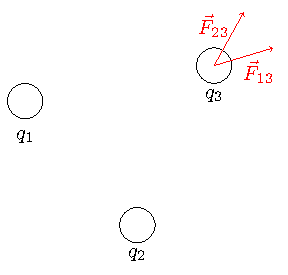
\includegraphics[width=0.55\linewidth]{2}
\par\end{center}

Entonces:

\[
\vec{F}_{13}=\frac{1}{4\pi\varepsilon_{0}}\frac{q_{1}q_{3}}{r_{13}^{2}}\hat{r}
\]

\[
\vec{F}_{23}=\frac{1}{4\pi\varepsilon_{0}}\frac{q_{2}q_{3}}{r_{23}^{2}}\hat{r}
\]

Además:

\[
\vec{F}_{3}=\vec{F}_{13}+\vec{F}_{23}
\]

En general:
\begin{prop}
\label{prop:superposici=0000F3n} El principio de superposición afirma
que cuando las ecuaciones de comportamiento que rigen un problema
físico son lineales, entonces el resultado de una medida o la solución
$O$ de un problema práctico relacionado con una magnitud extensiva
asociada al fenómeno, cuando están presentes los conjuntos de factores
causantes $I_{1},\dots,I_{k}$ con $k\in\mathbb{N}$, puede obtenerse
como la suma de los efectos de cada uno. 
\end{prop}
\begin{proof}
Sea $f:\mathbb{R}^{n}\longrightarrow\mathbb{R}^{m}$ una aplicación
lineal que relaciona dos magnitudes físicas $I$ (\textit{input})
y $O$ (\textit{output}). Supongamos, además, que contamos con $k\in\mathbb{N}$
subsistemas tales que cada uno produce una magnitud física de entrada
$I_{u}$. Queremos calcular cuál es el valor de $O$. Para ello:

\[
O=f\left(I_{1}+\dots+I_{k}\right)=f\left(\sum_{u=1}^{k}I_{u}\right)
\]
Y, como $f$ es lineal por hipótesis:
\[
O=\sum_{u=1}^{k}f\left(I_{u}\right)
\]
\end{proof}

\section{Ley de Coulomb}

Tenemos la siguiente situación:
\begin{center}
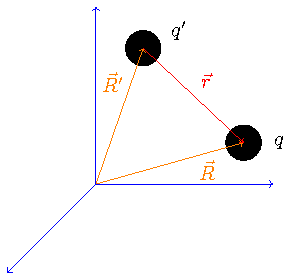
\includegraphics[width=0.55\linewidth]{1}
\par\end{center}

donde $q'$ y $q$ son cargas puntuales. Entonces:
\begin{ax}
\label{axm:Fqq'}La fuerza que la carga $q'$ ejerce sobre $q$ en
el vacío es:

\[
\vec{F}_{q'\rightarrow q}=\frac{1}{4\pi\varepsilon_{0}}\frac{q'q}{r^{2}}\hat{r}=\frac{1}{4\pi\varepsilon_{0}}\frac{q'q}{r^{3}}\vec{r}
\]

donde $\hat{r}=\frac{\vec{r}}{\left|\vec{r}\right|}$ y $\varepsilon_{0}\simeq8,85\;\frac{\text{F}}{\text{m}}$
es una constante llamada permitividad eléctrica del vacío y $r$ es
la distancia que separa ambas cargas. Nótese que esta fuerza será
atractiva si las cargas son del mismo signo y será repulsiva en caso
contrario.
\end{ax}
\begin{rem}
Por el principio de acción y reacción, sabemos que se cumple:

\[
\vec{F}_{q\rightarrow q'}=-\vec{F}_{q'\rightarrow q}
\]
\end{rem}

\subsection{¿Por qué sabemos que el denominador es $r^{2}$?}

Supongamos que el módulo de la fuerza eléctrica es proporcional a
la siguiente expresión:

\[
\left|\vec{F}_{q\rightarrow q'}\right|\propto\frac{1}{r^{2+\varepsilon}}
\]

A lo largo de la historia se ha llegado a las siguientes acotaciones:
\begin{enumerate}
\item Cavendish: $\left|\varepsilon\right|\le0,02$
\item Maxwell: $\left|\varepsilon\right|\le5\cdot10^{-5}$
\item Lawton (1936): $\left|\varepsilon\right|\le2\cdot10^{-9}$
\item Faller y Hill (1971): $\left|\varepsilon\right|\le2,7\cdot10^{-16}$
\end{enumerate}

\subsection{Comentarios sobre los límites de ley de Coulomb}

Para distancias grandes no hay problema, pues en ese caso la fuerza
electroestática se vuelve despreciable. Sin embargo, en el límite
inferior de la distancia sí que hay problemas, pues las fuerzas atómicas
empiezan a no ser despreciables. En general, consideraremos que podemos
aplicar la ley de Coulomb para valores de $r$ que cumplan $r>10^{-9}\;\text{m}$.

\section{Campo eléctrico}
\begin{defn}[Campo eléctrico]

Llamamos \textbf{campo eléctrico} al vector dado por la siguiente
fórmula límite:

\[
\vec{E}:=\lim_{q_{0}\rightarrow0}\frac{\vec{F}}{q_{0}}
\]
donde $\vec{F}$ es la suma de todas las fuerzas que actúan sobre
la carga $q_{0}$.
\end{defn}
\begin{center}
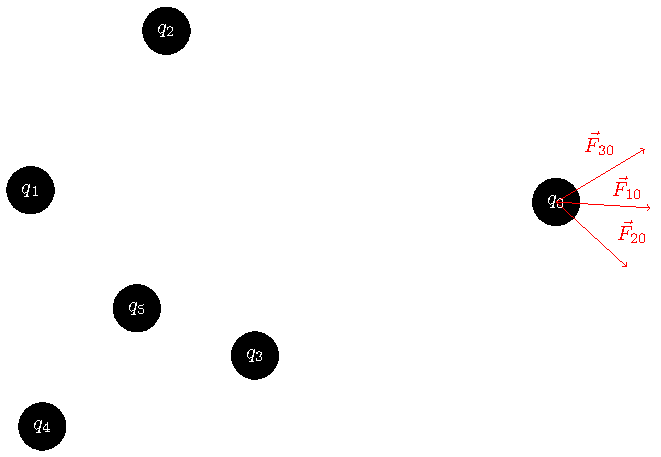
\includegraphics[width=0.7\linewidth]{3}
\par\end{center}

El concepto de límite está para indicar que la nueva carga añadida
es tan pequeña que su interacción con el resto de cargas del sistema
es despreciable. Nótese que la propia carga $q_{0}$ es necesaria
para el cálculo de $\vec{F}$, luego el límite es, en realidad, una
indeterminación ${\displaystyle \frac{0}{0}}$.

\subsection{Caso de una carga puntual}
\begin{prop}
\label{prop:Epuntual}El campo eléctrico $\vec{E}$ generado por una
carga puntual $q'$ en un punto $\vec{R}$ del espacio es:

\[
\vec{E}\left(\vec{R}\right)=\frac{1}{4\pi\varepsilon_{0}}\frac{q'}{r^{2}}\hat{r}
\]

donde $\vec{r}=\vec{R}-\vec{R}'$.
\end{prop}
\begin{proof}
Partimos del axioma \vref{axm:Fqq'}, de forma que:

\[
\vec{F}=\frac{1}{4\pi\varepsilon_{0}}\frac{q'q_{0}}{r^{2}}\hat{r}
\]

Aplicando la definición:

\[
\vec{E}\left(\vec{R}\right)=\lim_{q_{0}\rightarrow0}\frac{\frac{1}{4\pi\varepsilon_{0}}\frac{q'q_{0}}{r^{2}}\hat{r}}{q_{0}}=\frac{1}{4\pi\varepsilon_{0}}\frac{q'}{r^{2}}\hat{r}
\]
\end{proof}
\begin{notation}
Usaremos ' para denotar las cargas generadoras del campo. Utilizaremos
$\vec{R}'$ para referirnos a las posiciones de las cargas respecto
a nuestro sistema de coordenadas, mientras que usaremos $\vec{r}$
para las distancias relativas.
\end{notation}

\subsection{Caso de varias cargas puntuales}
\begin{cor}
El campo eléctrico generado por $n$ partículas puntuales en un punto
$\vec{R}$ del espacio es:

\[
\vec{E}\left(\vec{R}\right)=\sum_{i=1}^{n}\frac{1}{4\pi\varepsilon_{0}}\frac{q_{i}}{r_{i}^{2}}\hat{r}_{i}
\]

donde $\vec{r}_{i}=\vec{R}-\vec{R}'_{i}$.
\end{cor}
\begin{proof}
Se sigue trivialmente de la proposición anterior al aplicar el principio
de superposición.
\end{proof}
\begin{example}
Imaginemos:

\begin{center}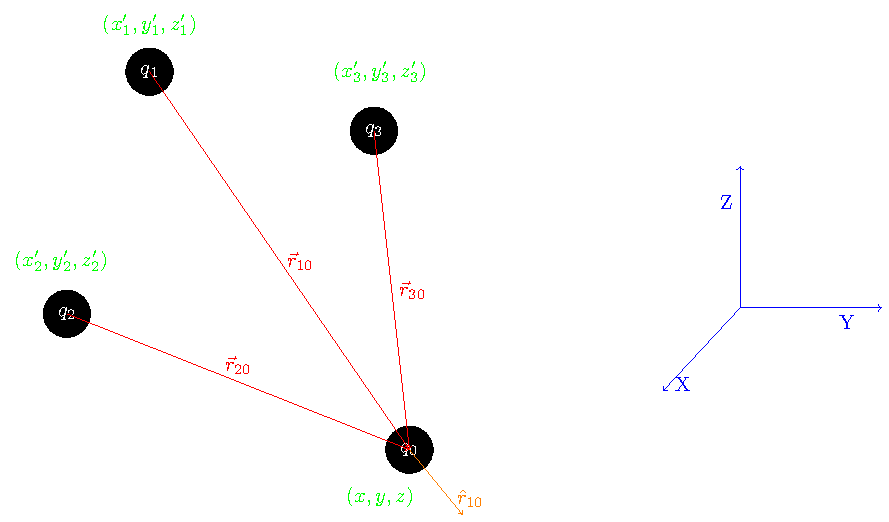
\includegraphics[width=0.8\linewidth]{4}\end{center}

En este caso:

\[
\vec{E}\left(\vec{R}\right)=\frac{1}{4\pi\varepsilon_{0}}\left(\frac{q_{1}}{r_{10}^{2}}\hat{r}_{10}+\frac{q_{2}}{r_{20}^{2}}\hat{r}_{20}+\frac{q_{3}}{r_{30}^{2}}\hat{r}_{30}\right)
\]

donde:

\[
r_{10}^{2}=\left(x_{0}-x'_{1}\right)^{2}+\left(y_{0}-y'_{1}\right)^{2}+\left(z_{0}-z'_{1}\right)^{2}
\]

En consecuencia:

\[
\left|\vec{r}_{10}\right|=\sqrt{\left(x_{0}-x'_{1}\right)^{2}+\left(y_{0}-y'_{1}\right)^{2}+\left(z_{0}-z'_{1}\right)^{2}}
\]

Por ende:

\[
\hat{r}_{10}=\frac{\vec{r}_{10}}{\left|\vec{r}_{10}\right|}=\frac{\left(x_{0}-x'_{1},y_{0}-y'_{1},z_{0}-z'_{1}\right)}{\sqrt{\left(x_{0}-x'_{1}\right)^{2}+\left(y_{0}-y'_{1}\right)^{2}+\left(z_{0}-z'_{1}\right)^{2}}}
\]
\end{example}
\begin{note}
En general se evitará el uso del subíndice $0$. Es decir, se usará
$r_{1}^{2}$ en vez de $r_{10}^{2}$; $x$, en vez de $x_{0}$ y así,
sucesivamente.
\end{note}

\subsection{Distribuciones de carga}
\begin{defn}
Llamamos función \textbf{densidad de carga volumétrica} a:
\[
\rho\left(\vec{R}'\right):=\frac{dQ}{dV}
\]
que nos devuelve la cantidad de carga $dQ$ que hay en un volumen
infinitesimal $dV$ situado en el punto $\vec{R}'$, siendo ${\displaystyle \left[\rho\right]=\frac{\text{C}}{\text{m}^{3}}}$.

En el caso de una superficie o de una distribución lineal, existen
igualmente:

\[
\begin{matrix}{\displaystyle \sigma\left(\vec{R}'\right):=\frac{dQ}{dS}} &  & {\displaystyle \lambda\left(\vec{R}'\right):=\frac{dQ}{dl}}\end{matrix}
\]
donde $\sigma\left(\vec{R}'\right)$ recibe el nombre de \textbf{densidad
de carga superficial} siendo ${\displaystyle \left[\sigma\right]=\frac{\text{C}}{\text{m}^{2}}}$
y $\lambda\left(\vec{R}'\right)$ recibe el nombre de \textbf{densidad
de carga lineal} siendo ${\displaystyle \left[\lambda\right]=\frac{\text{C}}{\text{m}}}$.
\end{defn}

\subsubsection{Distribución volumétrica}
\begin{prop}
\label{prop:EdV}El campo eléctrico generado por una distribución
de carga cuya densidad de carga volumétrica viene dada por una función
$\rho\left(\vec{R}'\right)$ responde a:

\[
\vec{E}\left(\vec{R}\right)=\frac{1}{4\pi\varepsilon_{0}}\iiint_{V'}\frac{\rho\left(\vec{R}'\right)}{r^{2}}\hat{r}dV'
\]
\end{prop}
\begin{proof}
Contemplemos una distribución de carga cualquiera:
\begin{center}
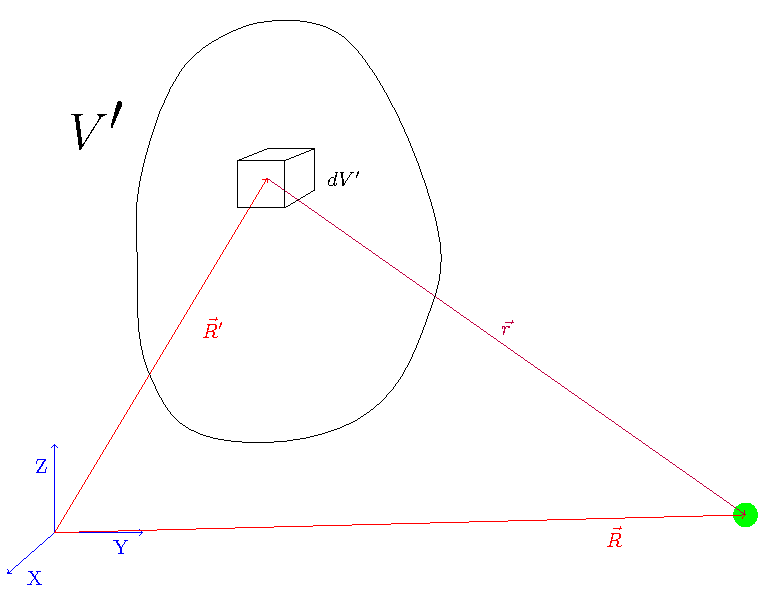
\includegraphics[width=0.6\linewidth]{5}
\par\end{center}

Nótese que $\vec{R}=\vec{R}'+\vec{r}\Leftrightarrow\vec{r}=\vec{R}-\vec{R}'$.
La densidad de carga del sólido viene dada por una función:

\[
\rho\left(\vec{R}'\right)=\frac{dQ}{dV'}\Leftrightarrow
\]

\[
\Leftrightarrow dQ=\rho\left(\vec{R}'\right)dV'
\]

El diferencial de volumen que tomo va a ser lo suficientemente pequeño
para poder considerarlo puntual. De esta forma:

\[
d\vec{E}\left(\vec{R}\right)=\frac{1}{4\pi\varepsilon_{0}}\frac{\rho\left(\vec{R}'\right)dV'}{r^{2}}\hat{r}
\]

A continuación, para hallar el campo total integramos al volumen:

\[
\vec{E}\left(\vec{R}\right)=\frac{1}{4\pi\varepsilon_{0}}\iiint_{V'}\frac{\rho\left(\vec{R}'\right)}{r^{2}}\hat{r}dV'
\]
\end{proof}

\subsubsection{Distribución superficial}
\begin{prop}
\label{prop:EdS}El campo eléctrico generado por una distribución
superficial de carga cuya densidad de carga superficial viene dada
por una función $\sigma\left(\vec{R}'\right)$ responde a:

\[
\vec{E}\left(\vec{R}\right)=\frac{1}{4\pi\varepsilon_{0}}\iint_{S'}\frac{\sigma\left(\vec{R}'\right)}{r^{2}}\hat{r}dS'
\]
\end{prop}
\begin{proof}
Imaginemos:

\begin{center}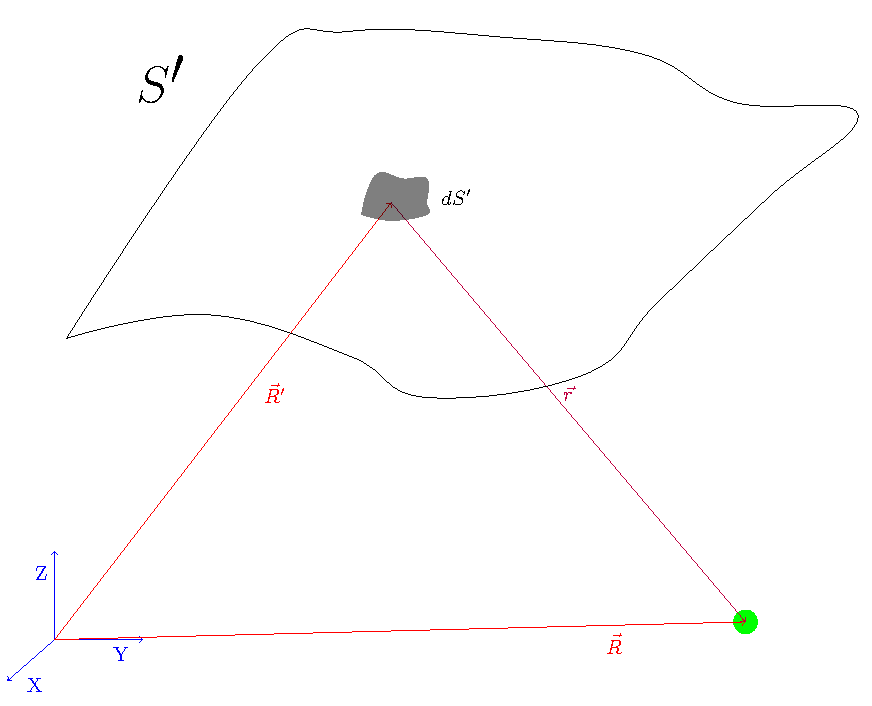
\includegraphics[width=0.6\linewidth]{6}\end{center}

Examinemos la función densidad de carga superficial:

\[
\sigma\left(\vec{R}'\right)=\frac{dQ}{dS'}
\]

De nuevo:

\[
dQ=\sigma\left(\vec{R}\right)dS'
\]

El campo que genera el diferencial de carga en el punto $\vec{R}$
es:

\[
d\vec{E}\left(\vec{R}\right)=\frac{1}{4\pi\varepsilon_{0}}\frac{\sigma\left(\vec{R}'\right)}{r^{2}}\hat{r}dS'
\]

Y, de forma similar al caso volumétrico:

\[
\vec{E}\left(\vec{R}\right)=\frac{1}{4\pi\varepsilon_{0}}\iint_{S'}\frac{\sigma\left(\vec{R}'\right)}{r^{2}}\hat{r}dS'
\]
\end{proof}

\subsubsection{Distribuciones lineales de carga}
\begin{prop}
\label{prop:Edl}El campo eléctrico generado por una distribución
lineal de carga cuya densidad viene dada por una función $\lambda\left(\vec{R}'\right)$
responde a:

\[
\vec{E}\left(\vec{R}\right)=\frac{1}{4\pi\varepsilon_{0}}\int_{l'}\frac{\lambda\left(\vec{R}'\right)\hat{r}}{r^{2}}dl'
\]
\end{prop}
\begin{proof}
Tenemos:
\begin{center}
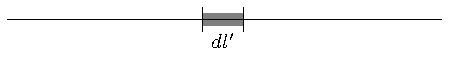
\includegraphics[width=1\linewidth]{7}
\par\end{center}

Todo es semejante a los casos anteriores:

\[
\lambda\left(\vec{R}'\right)=\frac{dQ}{dl'}
\]

\[
d\vec{E}\left(\vec{R}\right)=\frac{1}{4\pi\varepsilon_{0}}m\frac{\lambda\left(\vec{R}'\right)}{r^{2}}\hat{r}dl'
\]

Integrando a ambos lados llegamos a:

\[
\vec{E}\left(\vec{R}\right)=\frac{1}{4\pi\varepsilon_{0}}\int_{l'}\frac{\lambda\left(\vec{R}'\right)\hat{r}}{r^{2}}dl'
\]
\end{proof}
\begin{example}
Calculamos el campo generado por una varilla infinita.
\begin{center}
\includegraphics[width=0.6\linewidth]{\string"electro dibujo 1.5.4\string".pdf}
\par\end{center}

Sabemos:

\[
dQ=\lambda dz'
\]
El campo creado por el diferencial de carga es:

\[
d\vec{E}=\frac{1}{4\pi\varepsilon_{0}}\frac{\lambda dz'}{r^{2}}\hat{r}
\]
Por simetría sabemos que se va a anular el campo en el eje $z$, pues
por cada $dz'$ que existe por encima del punto, existe otro $dz'$
por debajo; de manera que los campos que se generan en la componente
$z$ se anulan entre sí.

Por tanto, definamos:

\[
dE_{R}:=\left|d\vec{E}\right|\cos\alpha
\]
Como ${\displaystyle \cos\alpha=\frac{R}{r}}$:

\[
dE_{R}\left(R\right)=\frac{1}{4\pi\varepsilon_{0}}\frac{\lambda dz'}{r^{2}}\frac{R}{r}
\]
El resultado final es:

\[
E_{R}\left(R\right)=2\int_{0}^{\infty}\frac{1}{4\pi\varepsilon_{0}}\frac{\lambda R}{r^{3}}dz'
\]
Como $r^{2}=R^{2}+z'^{2}$:

\[
E_{R}\left(R\right)=\frac{2\lambda R}{4\pi\varepsilon_{0}}\int_{0}^{\infty}\frac{dz'}{\left(R^{2}+z'^{2}\right)^{\frac{3}{2}}}=\frac{\lambda R}{2\pi\varepsilon_{0}}\left[\frac{z'}{R^{2}\sqrt{R^{2}+z'^{2}}}\right]_{z'=0}^{\infty}=
\]

\[
=\frac{\lambda R}{2\pi\varepsilon_{0}}\left(\frac{\overbrace{\frac{z'}{z'}}^{\xrightarrow{z'\rightarrow\infty}1}}{\underbrace{R^{2}\sqrt{\frac{R^{2}}{z'^{2}}+1}}_{\xrightarrow[z'\rightarrow\infty]{}R^{2}}}-0\right)=\frac{\lambda}{2\pi\varepsilon_{0}R}
\]
\end{example}

\subsubsection{Comentario final}
\begin{rem}
Nótese que las distribuciones de corrientes superficiales y lineales
no son más que un caso particular de corrientes volumétricas. Es decir,
si afirmamos que algo se cumple para distribuciones volumétricas,
debe cumplirse también para distribuciones superficiales y lineales.
El recíproco no es cierto.
\end{rem}

\section{Teorema de Gauss}
\begin{defn}
Se llama \textbf{superficie cerrada} a toda aquella que es compacta
(cerrada y acotada) y que no tiene frontera. La traducción intuitiva
a tres dimensiones es <<toda superficie que encierra un volumen>>.
\end{defn}
%
\begin{defn}
Llamamos \textbf{flujo de un vector} $\vec{A}$ a través de una superficie
$\vec{S}$ a:

\[
\Phi:=\iint_{S}\vec{A}\cdot d\vec{S}
\]
\begin{center}
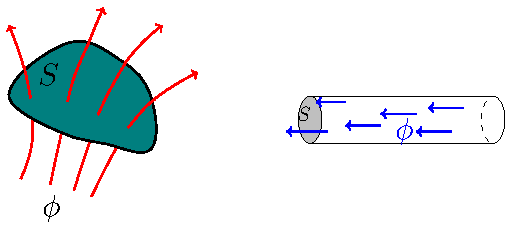
\includegraphics[width=0.8\linewidth]{flujo}
\par\end{center}

En una superficie cerrada, el vector $\vec{S}$ siempre va hacia fuera
de la superficie.
\end{defn}
\begin{thm}[Teorema de Gauss (forma integral)]
\label{thm:Gauss}

La integral del campo eléctrico a lo largo de una superficie cerrada
es igual a la carga total encerrada dentro de dicha superficie partido
por la permitividad eléctrica del vacío.

\[
\oiint_{S_{C}}\vec{E}\cdot d\vec{S}=\frac{Q_{T}}{\varepsilon_{0}}
\]

donde $S_{C}$ es una superficie cerrada, $Q_{T}$ es la carga encerrada
dentro de la superficie y $\varepsilon_{0}$ es la permitividad eléctrica
del vacío.
\end{thm}
%
\begin{note}
Este teorema se probará más adelante en su forma diferencial.
\end{note}
\begin{rem}
El teorema de Gauss nos será útil para hallar el campo eléctrico cuando
sepamos de antemano alguna propiedad del campo que nos permita despejarlo
de la ecuación (por ejemplo, si es constante a lo largo de la superficie).
\end{rem}
%
\begin{rem}
El teorema de Gauss es válido tal y como está escrito en cualquier
medio, no sólo en el vacío. Como veremos más adelante, la carga total
$Q_{T}$ que aparece incluye tanto la carga libre como la inducida.
\end{rem}
\begin{example}
Volvemos al ejemplo de la varilla. Como ya dijimos anteriormente,
en coordenadas cilíndricas el campo eléctrico no depende ni del ángulo
ni de la altura, únicamente de la distancia al hilo, es decir $\vec{E}=\mathfrak{F}\left(r,\cancel{\varphi},\cancel{z}\right)$.
Escogemos un cilindro de radio $r$ alrededor de la varilla y aplicamos
el teorema de Gauss:

\begin{center}\includegraphics[width=0.3\linewidth]{\string"electro dibujo 1.6\string".pdf}\end{center}

Descomponemos la integral en varias sumas:

\[
\oiint_{S_{C}}\vec{E}\cdot d\vec{S}=\iint_{\text{tapa superior}}\underbrace{\vec{E}\cdot d\vec{S}}_{\vec{E}\perp d\vec{S}\Rightarrow=0}+\iint_{\text{tapa inferior}}\underbrace{\vec{E}\cdot d\vec{S}}_{\vec{E}\perp d\vec{S}\Rightarrow=0}+\iint_{\text{superficie lateral}}\underbrace{\vec{E}\cdot d\vec{S}}_{\vec{E}\parallel d\vec{S}\Rightarrow=E\left(r\right)dS}=
\]

\[
=\iint_{\text{superficie lateral}}E\left(r\right)dS
\]

Como el campo es constante a lo largo de la superficie y la superficie
lateral del cilindro es $S=2\pi rh$:

\[
\iint_{\text{superficie lateral}}E\left(r\right)dS=E\left(r\right)2\pi rh
\]
Ahora, aplicamos el teorema de Gauss para despejar el campo:

\[
\oiint_{S_{C}}\vec{E}\cdot d\vec{S}=E\left(r\right)2\pi rh=\frac{\lambda h}{\varepsilon_{0}}\Leftrightarrow\vec{E}\left(r\right)=\frac{\lambda}{2\pi\varepsilon_{0}r}\hat{r}
\]
\end{example}

\subsection{Diferenciales en coordenadas cilíndricas}

\textbf{De longitud:}

\[
dl_{\text{círculo}}=rd\varphi
\]

\[
dl_{\text{altura}}=dz
\]

\[
d_{\text{radio}}=dr
\]

\textbf{De superficie:}

\[
dS_{\text{lateral}}=rd\varphi dz
\]

\[
dS_{\text{total}}=rdrd\varphi
\]

\textbf{De volumen:}

\[
dV=rdrd\varphi dz
\]


\subsection{Repaso de matemáticas}
\begin{defn}
\label{def:grad}Sea $\Omega$ un conjunto abierto en $\mathbb{R}^{3}$
y sea $\varphi:\Omega\longrightarrow\mathbb{R}$ una función escalar
tal que ${\displaystyle \exists\frac{\partial\varphi}{\partial j}\;\forall j=x,y,z}$.
Llamamos \textbf{gradiente} de $\varphi$ a:

\[
\text{grad}\varphi\equiv\frac{d}{d\vec{r}}\varphi\equiv\vec{\nabla}\varphi:=\left(\frac{\partial\varphi}{\partial x},\frac{\partial\varphi}{\partial y},\frac{\partial\varphi}{\partial z}\right)
\]
\end{defn}
%
\begin{defn}
\label{def:divergencia}Sea $\Omega$ un conjunto abierto en $\mathbb{R}^{3}$
y sea $\vec{A}:\Omega\longrightarrow\mathbb{R}^{3}$ una función vectorial
tal que ${\displaystyle \exists\frac{\partial A_{x}}{\partial x},\frac{\partial A_{y}}{\partial y},\frac{\partial A_{z}}{\partial z}}$.
Llamamos \textbf{divergencia} de $\vec{A}$ a:

\[
\text{div}\vec{A}=\vec{\nabla}\cdot\vec{A}:=\left(\frac{\partial}{\partial x},\frac{\partial}{\partial y},\frac{\partial}{\partial z}\right)\cdot\left(A_{x},A_{y},A_{z}\right)=\frac{\partial A_{x}}{\partial x}+\frac{\partial A_{y}}{\partial y}+\frac{\partial A_{z}}{\partial z}
\]
\end{defn}
%
\begin{defn}
\label{def:laplaciano}Sea $\Omega$ un conjunto abierto en $\mathbb{R}^{3}$
y sea $\varphi:\Omega\longrightarrow\mathbb{R}$ una función escalar
tal que ${\displaystyle \exists\frac{\partial^{2}\varphi}{\partial x^{2}},\frac{\partial^{2}\varphi}{\partial y^{2}},\frac{\partial^{2}\varphi}{\partial z^{2}}}$,
entonces llamamos \textbf{laplaciano} de $\varphi$ a:

\[
\nabla^{2}\varphi:=\vec{\nabla}\cdot\vec{\nabla}\left(\varphi\right)=\left(\frac{\partial}{\partial x},\frac{\partial}{\partial y},\frac{\partial}{\partial z}\right)\cdot\left(\frac{\partial\varphi}{\partial x},\frac{\partial\varphi}{\partial y},\frac{\partial\varphi}{\partial z}\right)=\frac{\partial^{2}\varphi}{\partial x^{2}}+\frac{\partial^{2}\varphi}{\partial y^{2}}+\frac{\partial^{2}\varphi}{\partial z^{2}}
\]
\end{defn}
%
\begin{defn}
Sea $\Omega$ un conjunto abierto en $\mathbb{R}^{3}$ y sea $\vec{A}:\Omega\longrightarrow\mathbb{R}^{3}$
una función vectorial tal que ${\displaystyle \exists\frac{\partial A_{i}}{\partial j}\;\forall i,j=x,y,}z$.
Llamamos \textbf{rotacional} de $\vec{A}$ a:

\[
\text{rot}\vec{A}\equiv\vec{\nabla}\times\vec{A}:=\left(\frac{\partial}{\partial x},\frac{\partial}{\partial y},\frac{\partial}{\partial z}\right)\times\left(A_{x},A_{y},A_{z}\right)=\left|\begin{matrix}\hat{i} & \hat{j} & \hat{k}\\
\frac{\partial}{\partial x} & \frac{\partial}{\partial y} & \frac{\partial}{\partial z}\\
A_{x} & A_{y} & A_{z}
\end{matrix}\right|
\]
\end{defn}
\begin{thm}[Teorema de la divergencia de Gauss-Ostrogradksy]
\label{thm:Divergencia}

Sea $\Omega$ un abierto en $\mathbb{R}^{3}$ y sea $\vec{A}:\Omega\longrightarrow\mathbb{R}^{3}$
una función vectorial diferenciable, $V$ un volumen y $S_{C}$ la
superficie cerrada que recubre dicho volumen. Entonces, la integral
al volumen $V$ de la divergencia de $\vec{A}$ coincide con la integral
de $\vec{A}$ a lo largo de la superficie $S_{C}$ que encierra dicho
volumen:

\[
\iiint_{V}\vec{\nabla}\cdot\vec{A}dV=\oiint_{S_{C}}\vec{A}d\vec{S}
\]
\end{thm}
\begin{defn}
\label{def:AngSol}Llamamos \textbf{ángulo sólido} al ángulo espacial
tal que su expresión diferencial es:

\[
d\Omega:=\frac{\hat{r}\cdot d\vec{S}}{r^{2}}=\frac{\vec{r}\cdot d\vec{S}}{r^{3}}
\]

Gráficamente:

\begin{center}\includegraphics[width=0.6\linewidth]{\string"electro dibujo 1.6.2 1\string".pdf}\end{center}

La idea del ángulo sólido\footnote{Más información en el siguiente enlace: \url{https://en.wikipedia.org/w/index.php?title=Solid_angle&oldid=880143402}.}
es el ángulo $2D$ (la <<anchura>> del cono) que se forma tras proyectar
la superficie sobre una esfera de radio unidad. Es decir, es una medida
del agujero que tendría que hacer en la esfera de radio unidad para
poder ver el $d\vec{S}$. Nótese que efectivamente es un ángulo, pues
es un parámetro adimensional.
\end{defn}
\begin{thm}[Teorema de Stokes]
\label{thm:Stokes}

Sea $\Omega$ un abierto en $\mathbb{R}^{3}$ y sea $\vec{A}:\Omega\longrightarrow\mathbb{R}^{3}$
una función vectorial tal que ${\displaystyle \exists\frac{\partial A_{i}}{\partial j}\;\forall i,j=x,y,z}$
y sea $S$ una superficie abierta. Entonces la integral del rotacional
de $\vec{A}$ a lo largo de la superficie $S$ tiene el mismo valor
que la integral de $\vec{A}$ a lo largo de la curva $C$ que delimita
la superficie abierta $S$.
\[
\iint_{S}\left(\vec{\nabla}\times\vec{A}\right)\cdot d\vec{S}=\oint_{C}\vec{A}\cdot d\vec{l}
\]
\end{thm}
\begin{rem}
Siempre debemos recorrer la curva siguiendo el sentido dado por la
regla de la mano derecha, donde el pulgar apunta en la dirección de
$d\vec{S}$.
\end{rem}

\subsection{Flujo eléctrico}
\begin{prop}
En términos del ángulo sólido, el flujo eléctrico cuando el campo
está generado por una única partícula puntual queda:

\[
\Phi=\oiint_{S_{C}}\vec{E}\cdot d\vec{S}=\frac{q}{4\pi\varepsilon_{0}}\iint d\Omega
\]
\end{prop}
\begin{proof}
Por la proposición \vref{prop:Epuntual}, sabemos que el campo eléctrico
generado por una carga puntual es:

\[
\vec{E}=\frac{1}{4\pi\varepsilon_{0}}\frac{q}{r^{2}}\hat{r}
\]

De manera que:

\[
\Phi=\oiint_{S_{C}}\vec{E}\cdot d\vec{S}=\frac{q}{4\pi\varepsilon_{0}}\iint\underbrace{\frac{\hat{r}\cdot d\vec{S}}{r^{2}}}_{=d\Omega}=\frac{q}{4\pi\varepsilon_{0}}\iint d\Omega
\]
\end{proof}
\begin{prop}
\label{prop:grad1/r}Siempre que sea $r\neq0$, el gradiente de ${\displaystyle \frac{1}{r}}$
respecto a las coordenadas sin primar puede expresarse como:

\[
\vec{\nabla}\left(\frac{1}{r}\right)=\frac{-\vec{r}}{r^{3}}=-\frac{\hat{r}}{r^{2}}
\]
\end{prop}
\begin{proof}
Expresamos $r$ en función de las coordenadas $x,y,z,x',y',z'$:
\[
r=\left|\vec{r}\right|=\sqrt{\left(x-x'\right)^{2}+\left(y-y'\right)^{2}+\left(z-z'\right)^{2}}
\]
Aplicamos la definición de gradiente (ver definición \vref{def:grad}):

\[
\vec{\nabla}\left(\frac{1}{r}\right)=\left(\frac{\partial}{\partial x}\left(\frac{1}{r}\right),\frac{\partial}{\partial y}\left(\frac{1}{r}\right),\frac{\partial}{\partial z}\left(\frac{1}{r}\right)\right)
\]
Calculemos $\frac{\partial}{\partial x}\left(\frac{1}{r}\right)$:

\[
\frac{\partial}{\partial x}\left(\frac{1}{r}\right)=-\frac{1}{2}\frac{1}{\left[\left(x-x'\right)^{2}+\left(y-y'\right)^{2}+\left(z-z'\right)^{2}\right]^{\frac{3}{2}}}2\left(x-x'\right)=
\]

\[
=\frac{x'-x}{\left[\left(x-x'\right)^{2}+\left(y-y'\right)^{2}+\left(z-z'\right)^{2}\right]^{\frac{3}{2}}}
\]
Análogamente:

\[
\frac{\partial}{\partial y}\left(\frac{1}{r}\right)=\frac{y'-y}{\left[\left(x-x'\right)^{2}+\left(y-y'\right)^{2}+\left(z-z'\right)^{2}\right]^{\frac{3}{2}}}
\]

\[
\frac{\partial}{\partial z}\left(\frac{1}{r}\right)=\frac{z'-z}{\left[\left(x-x'\right)^{2}+\left(y-y'\right)^{2}+\left(z-z'\right)^{2}\right]^{\frac{3}{2}}}
\]
Luego:

\[
\vec{\nabla}\left(\frac{1}{r}\right)=\frac{\overbrace{\left(x'-x,y'-y,z'-z\right)}^{=-\vec{r}}}{\left[\underbrace{\left(x-x'\right)^{2}+\left(y-y'\right)^{2}+\left(z-z'\right)^{2}}_{=r^{2}}\right]^{\frac{3}{2}}}=
\]

\[
=\frac{-\vec{r}}{r^{3}}=-\frac{\hat{r}}{r^{2}}
\]
\end{proof}
\begin{prop}
\label{prop:gradgrad'1/r}Siempre que sea $r\neq0$, el gradiente
de ${\displaystyle \frac{1}{r}}$ respecto a las coordenadas primadas
puede expresarse como:

\[
\vec{\nabla}'\left(\frac{1}{r}\right)=\frac{\vec{r}}{r^{3}}=\frac{\hat{r}}{r^{2}}=-\vec{\nabla}\left(\frac{1}{r}\right)
\]
\end{prop}
\begin{proof}
La demostración es casi idéntica a la anterior, sólo que cambian los
signos de las derivadas parciales.
\end{proof}
\begin{rem}
Nótese la diferencia de signos entre ambas versiones del gradiente.
\end{rem}

\paragraph{}

\subsection{Laplaciano de $\frac{1}{r}$~}
\begin{prop}
Siempre que sea $r\neq0$, el laplaciano de ${\displaystyle \frac{1}{r}}$
respecto a las coordenadas sin primar puede expresarse como:
\[
\nabla^{2}\left(\frac{1}{r}\right)=0
\]
\end{prop}
\begin{proof}
Por la proposición \vref{prop:grad1/r}:

\[
\vec{\nabla}\left(\frac{1}{r}\right)=\frac{\left(x'-x,y'-y,z'-z\right)}{\left[\left(x-x'\right)^{2}+\left(y-y'\right)^{2}+\left(z-z'\right)^{2}\right]^{\frac{3}{2}}}
\]
Ahora, sólo queda hallar la divergencia. Para ello, hallemos las derivadas
parciales:

\[
\frac{\partial}{\partial x}\left(\frac{x-x'}{\left[\left(x-x'\right)^{2}+\left(y-y'\right)^{2}+\left(z-z'\right)^{2}\right]^{\frac{3}{2}}}\right)=
\]

\[
=\frac{\left[\left(x-x'\right)^{2}+\left(y-y'\right)^{2}+\left(z-z'\right)^{2}\right]^{\frac{3}{2}}-\left(x-x'\right)\frac{3}{2}\left[\left(x-x'\right)^{2}+\left(y-y'\right)^{2}+\left(z-z'\right)^{2}\right]^{\frac{1}{2}}2\left(x-x'\right)}{\left[\left(x-x'\right)^{2}+\left(y-y'\right)^{2}+\left(z-z'\right)^{2}\right]^{3}}=
\]

\[
=\frac{\left(x-x'\right)^{2}+\left(y-y'\right)^{2}+\left(z-z'\right)^{2}-3\left(x-x'\right)^{2}}{\left[\left(x-x'\right)^{2}+\left(y-y'\right)^{2}+\left(z-z'\right)^{2}\right]^{\frac{5}{2}}}=
\]

\[
=\frac{r^{2}-3\left(x-x'\right)^{2}}{r^{5}}
\]
Análogamente:

\[
\frac{\partial}{\partial y}\left(\frac{y-y'}{\left[\left(x-x'\right)^{2}+\left(y-y'\right)^{2}+\left(z-z'\right)^{2}\right]^{\frac{3}{2}}}\right)=
\]

\[
=\frac{r^{2}-3\left(y-y'\right)^{2}}{r^{5}}
\]

\[
\frac{\partial}{\partial z}\left(\frac{z-z'}{\left[\left(x-x'\right)^{2}+\left(y-y'\right)^{2}+\left(z-z'\right)^{2}\right]^{\frac{3}{2}}}\right)=
\]

\[
=\frac{r^{2}-3\left(z-z'\right)^{2}}{r^{5}}
\]
Podemos ver que:

\[
\nabla^{2}\left(\frac{1}{r}\right)=\frac{3}{r^{5}}\left(r^{2}-\left[\left(x-x'\right)^{2}+\left(y-y'\right)^{2}+\left(z-z'\right)^{2}\right]\right)=\frac{3}{r^{5}}\left(r^{2}-r^{2}\right)=0
\]
\end{proof}

\subsection{Delta de Dirac}
\begin{defn}
Sea $f:\mathbb{R}\rightarrow\mathbb{R}$ la función dada por:
\[
f\left(x\right):=\left\{ \begin{matrix}0 & \text{ si } & x<x_{0}-\frac{a}{2}\\
\frac{1}{a} & \text{ si } & x_{0}-\frac{a}{2}\le x\le x_{0}+\frac{a}{2}\\
0 & \text{ si } & x>x_{0}+\frac{a}{2}
\end{matrix}\right.
\]
\begin{center}
\includegraphics[width=0.5\linewidth]{\string"electro dibujo 1.6.5\string".pdf}
\par\end{center}

Nótese que la función cumple:

\[
\int_{-\infty}^{\infty}f\left(x\right)dx=1
\]

Definimos la función \textbf{delta de Dirac} como:

\[
\delta\left(x-x_{0}\right):=\lim_{a\rightarrow0}f\left(x-x_{0}\right)
\]
\end{defn}
Esto nos permite la siguiente propiedad:
\begin{prop}[Propiedad de traslación de la delta]
\label{prop:TrasDelta}

Sean $x_{0}\in\mathbb{R}$ y $\begin{matrix}g: & \mathbb{R} & \longrightarrow & \mathbb{R}\\
 & x & \longrightarrow & g\left(x\right)
\end{matrix}$ una función continua cualquiera, entonces:

\[
\boxed{\int_{-\infty}^{\infty}\delta\left(x-x_{0}\right)g\left(x\right)dx=g\left(x_{0}\right)}
\]
\end{prop}
\begin{proof}
~
\[
\int_{-\infty}^{\infty}\delta\left(x-x_{0}\right)g\left(x\right)dx\overset{\text{def}}{=}\int_{-\infty}^{\infty}\lim_{a\rightarrow0}f\left(x-x_{0}\right)g\left(x\right)dx=
\]

\[
=\lim_{a\rightarrow0}\int_{x_{0}-\frac{a}{2}}^{x_{0}+\frac{a}{2}}f\left(x-x_{0}\right)g\left(x\right)dx=\lim_{a\rightarrow0}\int_{x_{0}-\frac{a}{2}}^{x_{0}+\frac{a}{2}}\frac{1}{a}g\left(x\right)dx=\lim_{a\rightarrow0}\frac{1}{a}\int_{x_{0}-\frac{a}{2}}^{x_{0}+\frac{a}{2}}g\left(x\right)dx=
\]
\[
=\lim_{a\rightarrow0}\frac{1}{a}ag\left(x_{0}\right)=g\left(x_{0}\right)
\]
\end{proof}
\begin{defn}
En tres dimensiones, la \textbf{delta de Dirac} se define como:

\[
\vec{\delta}\left(\vec{r}-\vec{r}_{0}\right):=\delta\left(x-x_{0}\right)\delta\left(y-y_{0}\right)\delta\left(z-z_{0}\right)
\]
\end{defn}

\subsection{Forma diferencial del Teorema de Gauss}
\begin{prop}
\label{prop:Lapl 1/r =00003D delta}El laplaciano de la función ${\displaystyle \frac{1}{r}}$
evaluado en un punto $\vec{R}$ es igual a menos cuatro pi veces la
delta de Dirac evaluada en la distancia relativa $\vec{r}=\vec{R}-\vec{R}'$.

\[
\nabla^{2}\left(\frac{1}{r}\right)\left(\vec{R}\right)=-4\pi\delta\left(\vec{r}\right)
\]
\end{prop}
\begin{proof}
Consideremos:

\[
\iiint_{V'}\nabla^{2}\left(\frac{1}{r}\right)dV'=\iiint_{V'}\vec{\nabla}\cdot\vec{\nabla}\left(\frac{1}{r}\right)dV'=\oiint_{S_{C}}\vec{\nabla}\left(\frac{1}{r}\right)d\vec{S}
\]
donde el último paso se debe al teorema de la divergencia (ver teorema
\vref{thm:Divergencia}). Por la proposición \vref{prop:grad1/r},
tenemos:

\[
\iiint_{V'}\nabla^{2}\left(\frac{1}{r}\right)dV'=-\oiint_{S_{C}}\frac{\vec{r}\cdot d\vec{S}}{r^{3}}=-\oiint_{S_{C}}d\Omega=-4\pi
\]
pues la integral a todos los posibles ángulos sólidos de $d\Omega$
es $4\pi$. A continuación, nótese que por la proposición \vref{prop:TrasDelta}:

\[
-4\pi=\iiint_{V'}-4\pi\delta\left(\vec{r}\right)dV'
\]
Por tanto:

\[
\iiint_{V'}\nabla^{2}\left(\frac{1}{r}\right)dV'=\iiint_{V'}-4\pi\delta\left(\vec{r}\right)dV'
\]
Como lo anterior debe cumplirse para cualquier volumen $V'$, llegamos
a que debe ser:
\[
\nabla^{2}\left(\frac{1}{r}\right)=-4\pi\delta\left(\vec{r}\right)
\]
\end{proof}
\begin{prop}
\label{prop:TGauss Int=00003D>Diff}La forma integral del teorema
de Gauss implica su forma diferencial. Es decir, si el flujo del campo
eléctrico a lo largo de una superficie cerrada $S_{C}$ es la carga
encerrada en dicha superficie partida por $\varepsilon_{0}$, entonces
la divergencia del campo eléctrico en cualquier punto $\vec{R}$ dentro
de dicha superficie $S_{C}$ debe ser la función densidad de carga
$\rho$ evaluada en dicho punto $\vec{R}$ partido por $\varepsilon_{0}$.

\[
\oiint_{S_{C}}\vec{E}\cdot d\vec{S}=\frac{Q_{T}}{\varepsilon_{0}}\Rightarrow\vec{\nabla}\cdot\vec{E}\left(\vec{R}\right)=\frac{\rho\left(\vec{R}\right)}{\varepsilon_{0}}
\]
\end{prop}
\begin{proof}
Primero,

Recordemos, ahora, que, por la proposición \vref{prop:Epuntual},
el campo generado por una distribución de carga es:

\[
\vec{E}\left(\vec{R}\right)=\frac{1}{4\pi\varepsilon_{0}}\iiint_{V'}\frac{\rho\left(\vec{R'}\right)\cdot\hat{r}}{r^{2}}dV'
\]
\begin{center}
\includegraphics[width=0.55\linewidth]{\string"electro dibujo 1.6.2 2\string".pdf}
\par\end{center}

Por tanto, tomando la divergencia a ambos lados, obtenemos:

\[
\vec{\nabla}\cdot\vec{E}\left(\vec{R}\right)=\frac{1}{4\pi\varepsilon_{0}}\vec{\nabla}\cdot\left(\iiint_{V'}\frac{\rho\left(\vec{R}'\right)\cdot\hat{r}}{r^{2}}dV'\right)
\]
Nótese que como la divergencia y la integral actúan respecto a coordenadas
diferentes, el orden de los operadores no importa, es decir, conmutan.
De forma que puedo cambiar el orden:

\[
\vec{\nabla}\cdot\vec{E}\left(\vec{R}\right)=\frac{1}{4\pi\varepsilon_{0}}\iiint_{V'}\vec{\nabla}\cdot\left(\frac{\rho\left(\vec{R}'\right)\cdot\hat{r}}{r^{2}}\right)dV'=\frac{1}{4\pi\varepsilon_{0}}\iiint_{V'}\rho\left(\vec{R}'\right)\vec{\nabla}\cdot\left(\frac{\hat{r}}{r^{2}}\right)dV'
\]
Ahora bien, por la proposición \vref{prop:grad1/r}, tenemos: 
\[
\frac{\hat{r}}{r^{2}}=-\vec{\nabla}\left(\frac{1}{r}\right)
\]
sustituyendo, tenemos:

\[
\vec{\nabla}\cdot\vec{E}\left(\vec{R}\right)=-\frac{1}{4\pi\varepsilon_{0}}\iiint_{V'}\rho\left(\vec{R}'\right)\underbrace{\vec{\nabla}\cdot\vec{\nabla}\left(\frac{1}{r}\right)}_{=\nabla^{2}\left(\frac{1}{r}\right)}dV'
\]
Por la definición de laplaciano (ver definición \vref{def:laplaciano}):
\[
\vec{\nabla}\cdot\vec{E}\left(\vec{R}\right)=-\frac{1}{4\pi\varepsilon_{0}}\iiint_{V'}\rho\left(\vec{R}'\right)\underbrace{\nabla^{2}\left(\frac{1}{r}\right)}_{=-4\pi\delta\left(\vec{r}\right)}dV
\]
Por la proposición \vref{prop:Lapl 1/r =00003D delta}:
\[
\vec{\nabla}\cdot\vec{E}\left(\vec{R}\right)=\frac{1}{4\pi\varepsilon_{0}}\iiint_{V'}\rho\left(\vec{R}'\right)4\pi\delta\left(\vec{r}\right)dV
\]
Recordando $\vec{r}=\vec{R}-\vec{R}'$:
\[
\vec{\nabla}\cdot\vec{E}\left(\vec{R}\right)=\frac{1}{\varepsilon_{0}}\iiint_{V'}\rho\left(\vec{R}'\right)\delta\left(\vec{R}-\vec{R}'\right)dV
\]
Por último, por la propiedad de traslación de la delta (ver proposición
\vref{prop:TrasDelta}):

\[
\vec{\nabla}\cdot\vec{E}\left(\vec{R}\right)=\frac{\rho\left(\vec{R}\right)}{\varepsilon_{0}}
\]
\end{proof}
\begin{rem}
\href{https://es.wikipedia.org/wiki/Ley_de_Gauss\#Forma_diferencial_e_integral_de_la_Ley_de_Gauss}{Aquí}\footnote{\url{https://es.wikipedia.org/w/index.php?title=Ley_de_Gauss&oldid=107400507\#Forma_diferencial_de_la_ley_de_Gauss}}
se ofrece una forma diferente de llegar al mismo resultado.
\end{rem}
Lo anterior nos permite enunciar:
\begin{thm}[Forma diferencial del teorema de Gauss]
\label{thm:GaussDiferencial}En cualquier punto $\vec{R}\in\mathbb{R}^{3}$
se cumple que la divergencia del campo eléctrico evaluada en dicho
punto $\vec{R}$ coincide con el valor de la función densidad de carga
evaluada en el punto $\vec{R}$ partido por $\varepsilon_{0}$.

\[
\boxed{\vec{\nabla}\cdot\vec{E}\left(\vec{R}\right)=\frac{\rho\left(\vec{R}\right)}{\varepsilon_{0}}}
\]
\end{thm}
\begin{rem}
Una divergencia positiva indica que las líneas de campo salen de la
carga, mientras que una divergencia negativa indica lo contrario.
\end{rem}
\begin{proof}[Demostración{*} (No entra)]
Recordando la proposición \vref{prop:Epuntual}, calculamos el campo
total en el punto $\vec{R}$ haciendo una integral a todas las cargas
puntuales infinitesimales que existen en el espacio (punto $\vec{R}'$
variable), obteniendo:

\[
\vec{E}\left(\vec{R}\right)=\frac{1}{4\pi\varepsilon_{0}}\iiint_{V}\frac{\rho\left(\vec{R}'\right)\left(\vec{R}-\vec{R}'\right)}{\left|\vec{R}-\vec{R}'\right|^{3}}\underbrace{d^{3}\vec{R}'}_{=dV}
\]

donde $\rho\left(\vec{R}'\right)$ es la función densidad de carga.
Si hacemos la divergencia a ambos lados de la ecuación y usamos la
proposición \vref{prop:Lapl 1/r =00003D delta}, llegamos a:

\[
\vec{\nabla}\cdot\vec{E}\left(\vec{R}\right)=\frac{1}{\varepsilon_{0}}\iiint_{V}\rho\left(\vec{R}'\right)\delta\left(\vec{R}-\vec{R}'\right)d^{3}\vec{R}'
\]
Y lo anterior, por la proposición \vref{prop:TrasDelta}, es equivalente
a:

\[
\vec{\nabla}\cdot\vec{E}\left(\vec{R}\right)=\frac{\rho\left(\vec{R}\right)}{\varepsilon_{0}}
\]
\end{proof}

\subsection{Obtención de la forma integral a partir de la forma diferencial}
\begin{prop}
\label{prop:TGauss Diff=00003D>Int}La forma diferencial del teorema
de Gauss implica su forma integral. Es decir, si para todo punto $\vec{R}$
contenido en el interior de una superficie cerrada $S_{C}$ se cumple
el teorema de Gauss en forma diferencial, entonces el flujo del campo
eléctrico a lo largo de la superficie $S_{C}$ toma el valor de la
carga encerrada en dicha superficie partido por $\varepsilon_{0}$.
\[
\vec{\nabla}\cdot\vec{E}\left(\vec{R}\right)=\frac{\rho\left(\vec{R}\right)}{\varepsilon_{0}}\Rightarrow\oiint_{S_{C}}\vec{E}\left(\vec{R}\right)d\vec{S}=\frac{Q_{T}}{\varepsilon_{0}}
\]
\end{prop}
\begin{proof}
Partimos del teorema \vref{thm:GaussDiferencial}:

\[
\vec{\nabla}\cdot\vec{E}\left(\vec{R}\right)=\frac{\rho\left(\vec{R}\right)}{\varepsilon_{0}}
\]
Hacemos la integral al volumen a ambos lados:

\[
\iiint_{V}\vec{\nabla}\cdot\vec{E}\left(\vec{R}\right)dV=\iiint_{V}\frac{\rho\left(\vec{R}\right)}{\varepsilon_{0}}dV
\]
Podemos ver fácilmente que el término de la derecha no es más que
la carga total presente en el objeto partido por $\varepsilon_{0}$.
Es decir:

\[
\iiint_{V}\frac{\rho\left(\vec{R}\right)}{\varepsilon_{0}}dV=\frac{1}{\varepsilon_{0}}\iiint_{V}\rho\left(\vec{R}\right)dV=\frac{Q_{T}}{\varepsilon_{0}}
\]
Ahora bien, por el teorema de la divergencia (\vref{thm:Divergencia}),
el término de la izquierda es igual a:

\[
\iiint_{V}\vec{\nabla}\cdot\vec{E}\left(\vec{R}\right)dV=\iint_{S_{C}}\vec{E}\left(\vec{R}\right)\cdot d\vec{S}
\]
Es decir, hemos llegado a:

\[
\oiint_{S_{C}}\vec{E}\left(\vec{R}\right)d\vec{S}=\frac{Q_{T}}{\varepsilon_{0}}
\]
\end{proof}
\begin{cor}
Gracias a las proposiciones \vref{prop:TGauss Int=00003D>Diff} y
\vref{prop:TGauss Diff=00003D>Int}, sabemos que las formulaciones
del teorema de Gauss en su forma integral (ver teorema \vref{thm:Gauss})
y en su forma diferencial (ver teorema \vref{thm:GaussDiferencial})
son equivalentes.
\end{cor}
\begin{prop}
\label{prop:Int Curv Cerrada de E =00003D 0}En electroestática, la
integral del campo eléctrico $\vec{E}$ generado por una distribución
volumétrica de cargas a través de una curva cerrada $C$ es siempre
nula.

\[
\oint_{C}\vec{E}\left(\vec{R}\right)\cdot d\vec{r}=0
\]
\end{prop}
\begin{proof}
Por la proposición \vref{prop:EdV}, sabemos que el campo eléctrico
generado por una distribución volumétrica de cargas viene dado por
la expresión:
\[
\vec{E}\left(\vec{R}\right)=\frac{1}{4\pi\varepsilon_{0}}\iiint_{V'}\frac{\rho\left(\vec{R}'\right)}{r^{2}}\hat{r}dV'
\]
Haciendo la integral a lo largo de una línea $C$ a ambos lados, tenemos:
\[
\oint_{C}\vec{E}\left(\vec{R}\right)\cdot d\vec{r}=\frac{1}{4\pi\varepsilon_{0}}\oint_{C}\left[\iiint_{V'}\frac{\rho\left(\vec{R}'\right)}{r^{2}}\hat{r}dV'\right]\cdot d\vec{r}
\]
Como las integrales se realizan a coordenadas diferentes, la integral
triple conmuta con la realizada a lo largo de la línea:
\[
\oint_{C}\vec{E}\left(\vec{R}\right)\cdot d\vec{r}=\frac{1}{4\pi\varepsilon_{0}}\iiint_{V'}\left[\rho\left(\vec{R}'\right)\oint_{C}\underbrace{\frac{\hat{r}}{r^{2}}}_{=\vec{\nabla}\left(\frac{1}{r}\right)}\cdot d\vec{r}\right]dV'
\]
Por la proposición \vref{prop:grad1/r}, tenemos:
\[
\oint_{C}\vec{E}\left(\vec{R}\right)\cdot d\vec{r}=\frac{1}{4\pi\varepsilon_{0}}\iiint_{V'}\left[\rho\left(\vec{R}'\right)\oint_{C}\underbrace{\vec{\nabla}\left(\frac{1}{r}\right)}_{=\frac{d}{d\vec{r}}\left(\frac{1}{r}\right)}\cdot d\vec{r}\right]dV'
\]
Por la definición de gradiente (ver definición \vref{def:grad}),
llegamos a:
\[
\oint_{C}\vec{E}\left(\vec{R}\right)\cdot d\vec{r}=\frac{1}{4\pi\varepsilon_{0}}\iiint_{V'}\left[\rho\left(\vec{R}'\right)\oint_{C}\frac{d\left(\frac{1}{r}\right)}{d\vec{r}}\cdot d\vec{r}\right]dV'=
\]
\[
=\frac{1}{4\pi\varepsilon_{0}}\iiint_{V'}\left[\rho\left(\vec{R}'\right)\oint_{C}d\left(\frac{1}{r}\right)\right]dV'=\frac{1}{4\pi\varepsilon_{0}}\iiint_{V'}\left(\rho\left(\vec{R}'\right)\left[\frac{1}{\rho}\right]_{r}^{r}\right)dV'
\]
donde el último paso se debe a que los extremos de una integral a
lo largo de un camino cerrado son el mismo punto. Así:
\[
\oint_{C}\vec{E}\left(\vec{R}\right)\cdot d\vec{r}=\frac{1}{4\pi\varepsilon_{0}}\iiint_{V'}\left(\rho\left(\vec{R}'\right)\left[\frac{1}{r}-\frac{1}{r}\right]\right)dV'=\frac{1}{4\pi\varepsilon_{0}}\iiint_{V'}\rho\left(\vec{R}'\right)0\,dV'=0
\]
\end{proof}
\begin{cor}
\label{cor:Campo El=0000E9ctrico Cons}El campo eléctrico $\vec{E}$
generado por una distribución volumétrica de carga es conservativo.
Es decir, se da:

\[
\vec{\nabla}\times\vec{E}\left(\vec{R}\right)=\vec{0}
\]
\end{cor}
\begin{proof}
Partimos de la proposición \vref{prop:Int Curv Cerrada de E =00003D 0}:
\[
\oint_{C}\vec{E}\left(\vec{R}\right)\cdot d\vec{r}=0
\]
Por el teorema de Stokes (\vref{thm:Stokes}), tenemos:

\[
0=\oint_{C}\vec{E}\left(\vec{R}\right)\cdot d\vec{r}=\iint_{S}\left(\vec{\nabla}\times\vec{E}\right)\cdot d\vec{S}
\]
para cualquier superficie abierta $S$ que se apoye en dicha curva.
\begin{center}
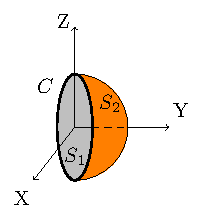
\includegraphics[width=0.5\linewidth]{superficies}
\par\end{center}

Como lo anterior se cumple para cualquier superficie abierta $S$
que se apoye en la curva $C$, necesariamente el núcleo de la integral
debe ser nulo:

\[
\vec{\nabla}\times\vec{E}\left(\vec{R}\right)=\vec{0}
\]
Como, además, el campo eléctrico generado por una distribución volumétrica
de cargas (ver proposición \vref{prop:EdV}) únicamente depende de
la posición $\vec{R}$, el campo eléctrico generado por una distribución
de cargas es conservativo.
\end{proof}
\begin{rem}
El corolario \vref{cor:Campo El=0000E9ctrico Cons}, nos va a permitir
replantear todo lo visto hasta la fecha utilizando funciones escalares
(la función potencial). De eso es de lo que va a tratar el siguiente
capítulo.
\end{rem}

\chapter{El potencial electroestático}

\thispagestyle{newchapter}
\begin{defn}
\label{def:PhiEl=0000E9ctrico}Llamamos \textbf{potencial eléctrico}
$\phi\left(\vec{R}\right)$ a la función escalar que cumple $-\vec{\nabla}\phi=\vec{E}$.
Esta definición tiene carácter general, para un campo $\vec{E}$ cualquiera,
siempre que sea conservativo.
\end{defn}

\section{Para una carga puntual}
\begin{prop}
\label{prop:PhiPuntual}El potencial eléctrico $\phi\left(\vec{R}\right)$
generado por una carga puntual $q'$ en un punto $\vec{R}$ del espacio
es:
\end{prop}
\[
\boxed{\phi\left(\vec{R}\right)=\frac{1}{4\pi\varepsilon_{0}}\frac{q'}{r}}
\]

\begin{proof}
Tenemos:
\begin{center}
\includegraphics[width=0.55\linewidth]{\string"electro dibujo 1.7.1\string".pdf}
\par\end{center}

Por la proposición \vref{prop:Epuntual}, el campo generado por una
carga puntual lo podemos expresar como:

\[
\vec{E}\left(\vec{R}\right)=\frac{1}{4\pi\varepsilon_{0}}q'\underbrace{\frac{\hat{r}}{r^{2}}}_{=-\vec{\nabla}\left(\frac{1}{r}\right)}
\]
Por la proposición \vref{prop:grad1/r}:
\[
\vec{E}\left(\vec{R}\right)=-\frac{q'}{4\pi\varepsilon_{0}}\vec{\nabla}\left(\frac{1}{r}\right)=-\vec{\nabla}\underbrace{\left(\frac{1}{4\pi\varepsilon_{0}}\frac{q'}{r}\right)}_{=:\phi\left(\vec{R}\right)}
\]
Por analogía con la definición de potencial eléctrico (ver definición
\vref{def:PhiEl=0000E9ctrico}):
\[
\vec{E}\left(\vec{R}\right)=-\vec{\nabla}\phi\left(\vec{R}\right)
\]
Donde $\phi\left(\vec{R}\right)$ es la función escalar:

\[
\phi\left(\vec{R}\right)=\frac{1}{4\pi\varepsilon_{0}}\frac{q'}{r}
\]
\end{proof}
\begin{rem}
Por las propiedades equivalentes de una una fuerza conservativa, siempre
que $\vec{\nabla}\times\vec{E}=\vec{0}$, existe una función $\phi\left(\vec{R}\right)$
tal que $\vec{E}\left(\vec{R}\right)=-\vec{\nabla}\phi\left(\vec{R}\right)$.
\end{rem}

\section{Para una distribución de carga}
\begin{prop}
\label{prop:PhiV}El potencial eléctrico $\phi\left(\vec{R}\right)$
generado por una distribución volumétrica de carga es:
\end{prop}
\begin{equation}
\phi\left(\vec{R}\right)=\frac{1}{4\pi\varepsilon_{0}}\iiint_{V'}\frac{\rho\left(\vec{R}'\right)}{r}dV'
\end{equation}

\begin{proof}
Fijémonos en el dibujo:
\begin{center}
\textcolor{green}{\includegraphics[width=0.55\linewidth]{\string"electro dibujo 1.7.2\string".pdf}}
\par\end{center}

Por la proposición \vref{prop:EdV}, sabemos que el campo en un punto
$\vec{R}$ viene dado por:

\[
\vec{E}\left(\vec{R}\right)=\frac{1}{4\pi\varepsilon_{0}}\iiint_{V'}\frac{\rho\left(\vec{R}'\right)\hat{r}dV'}{r^{2}}
\]
Por la proposición \vref{prop:grad1/r}, tenemos:
\[
\vec{E}\left(\vec{R}\right)=-\frac{1}{4\pi\varepsilon_{0}}\iiint_{V'}\rho\left(\vec{R}'\right)\vec{\nabla}\left(\frac{1}{r}\right)dV'
\]
Como el gradiente es respecto a las coordenadas sin primar y la función
densidad volumétrica de carga $\rho$ se evalúa sobre las coordenadas
primadas, $\rho\left(\vec{R}'\right)$ es constante para el gradiente
y podemos meterlo dentro del gradiente.

\[
\vec{E}\left(\vec{R}\right)=-\frac{1}{4\pi\varepsilon_{0}}\iiint_{V'}\vec{\nabla}\left(\frac{\rho\left(\vec{R}'\right)}{r}\right)dV'
\]
Como la integral se hace respecto a las coordenadas primadas y el
gradiente se hace respecto a las coordenadas sin primar, ambos operadores
conmutan:
\[
\vec{E}\left(\vec{R}\right)=-\vec{\nabla}\underbrace{\left(\frac{1}{4\pi\varepsilon_{0}}\iiint_{V'}\frac{\rho\left(\vec{R}'\right)}{r}dV'\right)}_{=:\phi\left(\vec{R}\right)}
\]
Es decir:

\[
\phi\left(\vec{R}\right)=\frac{1}{4\pi\varepsilon_{0}}\iiint_{V'}\frac{\rho\left(\vec{R}'\right)}{r}dV'
\]

\[
\vec{E}\left(\vec{R}\right)=-\vec{\nabla}\phi\left(\vec{R}\right)
\]
\end{proof}
\begin{rem}
Nótese que diferenciando a ambos lados de la expresión para el potencial
dada por la proposición \vref{prop:PhiV}, tenemos:
\[
d\phi\left(\vec{R}\right)=\frac{1}{4\pi\varepsilon_{0}}\frac{\rho\left(\vec{R}'\right)}{r}dV'
\]
Usaremos esto para calcular el potencial generado por distribuciones
de carga volumétricas en la práctica.
\end{rem}

\section{El significado físico del potencial}
\begin{prop}
Tenemos una región del espacio donde tenemos definido un campo eléctrico
$\vec{E}\left(\vec{R}\right)$ y su potencial asociado $\phi\left(\vec{R}\right)$.
Entonces el trabajo realizado por el campo eléctrico para desplazar
una carga desde un punto $\vec{R}_{1}$ hasta otro punto $\vec{R}_{2}$
es:

\[
W_{\vec{R}_{1}\rightarrow\vec{R}_{2}}=-q\left[\phi\left(\vec{R}_{2}\right)-\phi\left(\vec{R}_{1}\right)\right]
\]
\begin{center}
\includegraphics[width=0.4\linewidth]{\string"electro dibujo 1.7.3\string".pdf}
\par\end{center}

\end{prop}
\begin{proof}
Por el teorema del trabajo en su forma diferencial, tenemos:
\[
\dbar W_{\vec{R}_{1}\rightarrow\vec{R}_{2}}=\vec{F}\cdot d\vec{r}=q\vec{E}\cdot d\vec{r}\Leftrightarrow W_{1\rightarrow2}=\int_{\vec{R}_{1}}^{\vec{R}_{2}}q\vec{E}\cdot d\vec{r}
\]
Por la definición de potencial eléctrico (ver definición \vref{def:PhiEl=0000E9ctrico}),
podemos reescribir lo anterior como:
\[
\dbar W_{\vec{R}_{1}\rightarrow\vec{R}_{2}}=-q\int_{\vec{R}_{1}}^{\vec{R}_{2}}\vec{\nabla}\phi\cdot d\vec{r}
\]
Por definición de gradiente (ver definición \vref{def:grad}):

\[
\dbar W_{\vec{R}_{1}\rightarrow\vec{R}_{2}}=-q\int_{\vec{R}_{1}}^{\vec{R}_{2}}\frac{d\phi}{d\vec{r}}\cdot d\vec{r}=-q\int_{\vec{R}_{1}}^{\vec{R}_{2}}d\phi=-q\left[\phi\left(\vec{R}_{2}\right)-\phi\left(\vec{R}_{1}\right)\right]
\]
\end{proof}

\section{Ecuaciones de Poisson y Laplace}
\begin{thm}[Ecuación de Poisson]
\label{thm:Poisson}El laplaciano del potencial eléctrico en un punto
$\vec{R}$ es igual a menos la densidad de carga volumétrica $\rho$
evaluada en dicho punto $\vec{R}$ partido por $\varepsilon_{0}$.

\[
\boxed{\nabla^{2}\phi\left(\vec{R}\right)=-\frac{\rho\left(\vec{R}\right)}{\varepsilon_{0}}}
\]
\end{thm}
\begin{proof}
Por el teorema de Gauss en forma diferencial (ver teorema \vref{thm:GaussDiferencial})
sabemos:

\[
\vec{\nabla}\cdot\vec{E}\left(\vec{R}\right)=\frac{\rho\left(\vec{R}\right)}{\varepsilon_{0}}
\]
Por la definición de potencial eléctrico (ver definición \vref{def:PhiEl=0000E9ctrico}),
tenemos $\vec{E}\left(\vec{R}\right)=-\vec{\nabla}\phi$; sustituyendo
llegamos a:

\[
\vec{\nabla}\cdot\left(-\vec{\nabla}\phi\right)=\frac{\rho\left(\vec{R}\right)}{\varepsilon_{0}}\Leftrightarrow\vec{\nabla}\cdot\vec{\nabla}\phi=-\frac{\rho\left(\vec{R}\right)}{\varepsilon_{0}}
\]

\[
\Leftrightarrow\nabla^{2}\phi=-\frac{\rho\left(\vec{R}\right)}{\varepsilon_{0}}
\]
\end{proof}
\begin{rem}
En coordenadas cartesianas, la ecuación de Poisson se puede expresar
como:

\[
\frac{d^{2}\phi}{dx^{2}}+\frac{d^{2}\phi}{dy^{2}}+\frac{d^{2}\phi}{dz^{2}}=-\frac{\rho\left(x,y,z\right)}{\varepsilon_{0}}
\]
\end{rem}
\begin{cor}[La ecuación de Laplace]
\label{cor:Lapalce}Si la densidad de carga volumétrica es nula en
un punto $\vec{R}$, entonces el laplaciano del potencial se anula
en ese punto.

\[
\boxed{\nabla^{2}\phi\left(\vec{R}\right)=0}
\]
\end{cor}
\begin{proof}
Se sigue trivialmente del teorema \vref{thm:Poisson} sustituyendo
$\rho\left(\vec{R}\right)$ por $0$.
\end{proof}

\subsection{\label{subsec:Sol Ec Laplace}{*}Resolución en cartesianas (No entra):}

Deseamos resolver la ecuación de Laplace en cartesianas:

\[
\nabla^{2}\phi=\frac{d^{2}\phi}{dx^{2}}+\frac{d^{2}\phi}{dy^{2}}+\frac{d^{2}\phi}{dz^{2}}=0
\]
Tenemos garantizado que la solución de la ecuación diferencial (lo
probamos más adelante) es única y dicha solución debe ser de la forma:

\[
\phi\left(x,y,z\right)=X\left(x\right)Y\left(y\right)Z\left(z\right)
\]
donde $X=\mathfrak{F}\left(x\right)$, $Y=\mathfrak{F}\left(y\right)$
y $Z=\mathfrak{F}\left(z\right)$ (la $\mathfrak{F}$ indica <<función
de>>). Esto se llama separación de variables. Entonces, debe ser:

\[
\frac{d^{2}\phi}{dx^{2}}=\frac{d}{dx}\left[\frac{d}{dx}\left(XYZ\right)\right]=\frac{d}{dx}\left[YZ\frac{dX}{dx}\right]=YZ\frac{d^{2}X}{dx^{2}}
\]
Haciendo esto para todas las coordenadas, obtenemos:

\[
YZ\frac{d^{2}X}{dx^{2}}+XZ\frac{d^{2}Y}{dy^{2}}+XY\frac{d^{2}Z}{dz^{2}}=0
\]

Descartando la solución trivial ($X\left(x\right)=0$, $Y\left(y\right)=0$,
$Z\left(z\right)=0$), obtenemos:

\[
\frac{1}{X}\frac{d^{2}X}{dx^{2}}+\frac{1}{Y}\frac{d^{2}Y}{dy^{2}}+\frac{1}{Z}\frac{d^{2}Z^{2}}{dz^{2}}=0\Leftrightarrow
\]

\[
\Leftrightarrow\frac{1}{Y}\frac{d^{2}Y}{dy^{2}}+\frac{1}{Z}\frac{d^{2}Z}{dz^{2}}=-\frac{1}{X}\frac{d^{2}X}{dx^{2}}
\]
Como 
\[
k_{1}^{2}:=-\frac{1}{X}\frac{d^{2}X}{dx^{2}}\neq\mathfrak{F}\left(y,z\right)
\]
obtenemos la ecuación diferencial:

\[
-\frac{1}{X}\frac{d^{2}X}{dx^{2}}=k_{1}^{2}\Leftrightarrow\frac{d^{2}X}{dx^{2}}=-k_{1}^{2}X
\]
Suponiendo $k_{1}^{2}\neq0$, sabemos que la solución de esta ecuación
diferencial es:

\[
X\left(x\right)=Ae^{\pm ik_{1}x}
\]
Si $k_{1}=0$, la solución es de la forma:

\[
X\left(x\right)=Bx+C
\]

En consecuencia, obtenemos:

\[
\frac{1}{Y}\frac{d^{2}Y}{dy^{2}}+\frac{1}{Z}\frac{d^{2}Z}{dz^{2}}=k_{1}^{2}\Leftrightarrow\frac{1}{Y}\frac{d^{2}Y}{dy^{2}}=k_{1}^{2}-\frac{1}{Z}\frac{d^{2}Z}{dz^{2}}
\]
Ahora, como 
\[
-k_{2}^{2}:=k_{1}^{2}-\frac{1}{Z}\frac{d^{2}Z}{dz^{2}}\neq\mathfrak{F}\left(y\right)
\]
podemos hacer lo mismo que antes, obteniendo la solución:

\[
Y\left(y\right)\left\{ \begin{matrix}A'e^{\pm ik_{2}y} & \text{ si } & k_{2}\neq0\\
B'y+C' & \text{ si } & k_{2}=0
\end{matrix}\right.
\]

Ahora, finalmente, tendríamos:

\[
\frac{1}{Z}\frac{d^{2}Z}{dz^{2}}=k_{1}^{2}+k_{2}^{2}=:k_{3}^{2}
\]
cuya solución es:

\[
Z\left(z\right)\left\{ \begin{matrix}A''e^{\pm jk_{2}z} & \text{ si } & k_{3}\neq0\\
B''z+C'' & \text{ si } & k_{3}=0
\end{matrix}\right.
\]

En conclusión, la solución general es una combinación lineal de senos
y consenos trigonométricos e hiperbólicos.
\begin{example}[{*}Ejemplo de resolución de la ecuación diferencial (No entra)]

Tenemos la siguiente situación:
\begin{center}
\includegraphics[width=0.7\linewidth]{\string"voluntaria \string".pdf}
\par\end{center}

Conocemos las siguientes condiciones de contorno:
\begin{enumerate}
\item $\phi=0$ cuando $y=0$ o $y=b$.
\item Cuando $x=0$, $\phi=\mathfrak{F}!\left(y\right)$, es decir $\phi$
depende únicamente de $y$.
\item Cuando $x\rightarrow\infty$, $\phi\left(x,y,z\right)=0$.
\end{enumerate}
Sean $\alpha,\beta,\gamma\neq0$, entonces la solución general en
ese caso es:

\[
\phi\left(x,y,z\right)=\sum_{\alpha,\beta,\gamma}\left[a_{1}\left(\alpha\right)e^{\alpha x}+a_{2}\left(\alpha\right)e^{-\alpha x}\right]\left[b_{1}\left(\beta\right)e^{\beta y}+b_{2}\left(\beta\right)e^{-\beta y}\right]\left[c_{1}\left(\gamma\right)e^{\varphi z}+c_{2}\left(\gamma\right)e^{-\gamma z}\right]
\]
Si $\alpha,\beta$ o $\gamma$ fuesen alguno de ellos nulos, sustituiríamos
el término correspondiente por un término del estilo $c'_{1}z+c'_{2}$.

Por simetría traslacional de nuestro problema, el potencial no puede
depender de $z$, eso nos implica que la parte de $\phi$ que depende
de $z$ debe ser obligatoriamente de la forma:

\[
Z\left(z\right)=c'_{1}z+c'_{2}
\]
Pero como el potencial $\phi\left(x,y,z\right)=X\left(x\right)Y\left(y\right)Z\left(z\right)$
no puede depender de $z$, necesariamente:

\[
c'_{1}=0
\]
Y, en consecuencia:

\[
Z\left(z\right)=c'_{2}
\]

\[
\phi\left(x,y,z\right)=\sum_{\alpha,\beta}\left[a_{1}\left(\alpha\right)e^{\alpha x}+a_{2}\left(\alpha\right)e^{-\alpha x}\right]\left[b_{1}\left(\beta\right)e^{\beta y}+b_{2}\left(\beta\right)e^{-\beta y}\right]c'_{2}
\]

Para poder olvidarnos de $c'_{2}$, cambiamos los coeficientes dependientes
de $\alpha$ y $\beta$:

\[
\phi\left(x,y,z\right)=\sum_{\alpha,\beta}\left[a'_{1}\left(\alpha\right)e^{\alpha x}+a'_{2}\left(\alpha\right)e^{-\alpha x}\right]\left[b'_{1}\left(\beta\right)e^{\beta y}+b'_{2}\left(\beta\right)e^{-\beta y}\right]
\]
Sabemos que debe cumplirse (por las condiciones de las $k$ que hallamos
antes en la deducción de la solución general):

\[
\alpha^{2}+\beta^{2}=0
\]
Suponiendo $\alpha\in\mathbb{R}$:

\[
-\alpha^{2}=\beta^{2}\Leftrightarrow i\alpha=\beta
\]
Y, por tanto:

\[
\phi\left(x,y,z\right)=\sum_{\alpha}\left[a'_{1}\left(\alpha\right)e^{\alpha x}+a'_{2}\left(\alpha\right)e^{-\alpha x}\right]\left[b'_{1}\left(i\alpha\right)e^{i\alpha y}+b'_{2}\left(i\alpha\right)e^{-i\alpha y}\right]
\]
Suponiendo $\alpha>0$; por la condición de que el potencial en el
infinito debe ser cero, para que la función no <<explote>>, obligatoriamente
debe ser:

\[
a'_{1}\left(\alpha\right)=0
\]

Luego la solución es necesariamente de la forma:

\[
\phi\left(x,y,z\right)=\sum_{\alpha}a'_{2}\left(\alpha\right)e^{-\alpha x}\left[b'_{1}\left(i\alpha\right)e^{i\alpha y}+b'_{2}\left(i\alpha\right)e^{-i\alpha y}\right]
\]
Ahora, de nuevo, podemos hacer el mismo truco de antes y eliminarnos
la constante $a'_{2}\left(\alpha\right)$, metiéndola por la propiedad
distributiva en el corchete, cambiando las constantes $b'_{1}$ y
$b'_{2}$. Nos queda:

\[
\phi\left(x,y,z\right)=\sum_{\alpha}e^{-\alpha x}\left[b''_{1}\left(i\alpha\right)e^{i\alpha y}+b''_{2}\left(i\alpha\right)e^{-i\alpha y}\right]
\]
Ahora, vamos a imponer:

\[
\phi\left(x,0\right)=0
\]
Como la exponencial nunca se anula debe ser:

\[
b''_{1}\left(i\alpha\right)+b''_{2}\left(i\alpha\right)=0\Leftrightarrow b''_{1}=-b''_{2}
\]

De manera que nuestra solución se simplifica a:

\[
\phi\left(x,y,z\right)=\sum_{\alpha}b''_{1}\left(i\alpha\right)e^{-\alpha x}\left[e^{i\alpha y}-e^{-i\alpha y}\right]
\]
Sabiendo:

\[
\sin\theta=\frac{e^{i\theta}-e^{-i\theta}}{2i}
\]
Llegamos a:

\[
\phi\left(x,y,z\right)=\sum_{\alpha}b''_{1}\left(i\alpha\right)e^{-\alpha x}2i\sin\alpha y
\]
Ahora llamando $b'''_{1}\left(i\alpha\right):=b''_{1}2i$, obtenemos:

\[
\phi\left(x,y,z\right)=\sum_{\alpha}b'''_{1}e^{-\alpha x}\sin\alpha y
\]

Ahora aplicamos otra condición de contorno: $\phi\left(x,b\right)=0$.
Para ello debe ser:

\[
\sin\alpha b=0\Leftrightarrow\alpha b=n\pi\Leftrightarrow\alpha=\frac{n\pi}{b}
\]
Así, nuestra solución queda:

\[
\phi\left(x,y,z\right)=\sum_{n=0}^{\infty}B_{n}e^{-\frac{n\pi}{\beta}x}\sin\left(\frac{n\pi}{b}y\right)
\]
donde $B_{n}$ es una constante. A continuación, aplicamos la condición
restante $\phi\left(0,y\right)=\mathfrak{F}\left(y\right)$:

\[
\phi\left(0,y\right)=\sum_{n=0}^{\infty}B_{n}\sin\left(\frac{n\pi}{b}y\right)
\]
Multiplicamos por $\sin\left(\frac{m\pi}{b}y\right)$ a ambos lados
donde $m\in\mathbb{N}$.

\[
\phi\left(0,y\right)\sin\left(\frac{m\pi}{b}y\right)=\sum_{n=0}^{\infty}B_{n}\sin\left(\frac{n\pi}{b}y\right)\sin\left(\frac{m\pi}{b}y\right)
\]
Ahora integramos a ambos lados respecto a $y$ entre $0$ y $b$:

\[
\int_{0}^{b}\phi\left(0,y\right)\sin\left(\frac{m\pi}{b}y\right)dy=\sum_{n=0}^{\infty}\int_{0}^{b}B_{n}\sin\left(\frac{n\pi}{b}y\right)\sin\left(\frac{m\pi}{b}y\right)
\]
Utilizando la conocidísima identidad:

\[
\int_{a}^{b}\sin\left(\frac{m\pi y}{b}\right)\sin\left(\frac{n\pi y}{b}\right)dy=\frac{1}{2}b\delta_{mn}
\]
llegamos a:

\[
\int_{0}^{b}\phi\left(0,y\right)\sin\left(\frac{m\pi}{b}y\right)dy=\frac{1}{2}bB_{m}\Leftrightarrow
\]

\[
\Leftrightarrow B_{m}=\frac{2}{b}\int_{0}^{b}\phi\left(0,y\right)\sin\left(\frac{m\pi}{b}y\right)dy
\]

En consecuencia, obtenemos:

\[
\phi\left(x,y,z\right)=\sum_{n=0}^{\infty}B_{n}e^{-\frac{n\pi}{b}x}\sin\left(\frac{n\pi}{b}y\right)
\]
donde:

\[
B_{n}=\frac{2}{b}\int_{0}^{b}\phi\left(0,y\right)\sin\left(\frac{n\pi}{b}y\right)dy
\]
Nótese que si $n$ es par $B_{n}=0$; mientras que cuando $n$ es
impar:

\[
B_{n}=\frac{4V_{0}}{n\pi}
\]

A continuación, definimos $V_{0}:=\phi\left(0,y\right)$. Con esto,
podemos escribir:

\[
\phi\left(x,y\right)=\frac{4V_{0}}{\pi}\sum_{n=1}^{\infty}\frac{1}{2n-1}\sin\left[\frac{\left(2n-1\right)\pi}{b}y\right]e^{-\frac{\left(2n-1\right)\pi}{b}x}
\]
que es la solución a nuestro problema.

Ahora, podríamos hallar el campo, simplemente aplicando la definición
\vref{def:PhiEl=0000E9ctrico}:

\[
E_{x}=-\frac{\partial\phi}{\partial x}=\frac{4V_{0}}{\pi}\sum_{n=1}^{\infty}\frac{1}{2n-1}\sin\left[\frac{\left(2n-1\right)\pi}{b}y\right]\frac{\left(2n-1\right)\pi}{b}e^{-\frac{\left(2n-1\right)\pi}{b}x}=
\]

\[
=\frac{4V_{0}}{b}\sum_{n=1}^{\infty}\sin\left[\frac{\left(2n-1\right)\pi}{b}y\right]e^{-\frac{\left(2n-1\right)\pi}{b}x}
\]

\[
E_{y}=-\frac{\partial\phi}{\partial y}=\frac{4V_{0}}{\pi}\sum_{n=1}^{\infty}\frac{1}{2n-1}\frac{\left(2n-1\right)\pi}{b}\cos\left[\frac{\left(2n-1\right)\pi}{b}y\right]e^{-\frac{\left(2n-1\right)\pi}{b}x}=
\]

\[
=\frac{4V_{0}}{b}\sum_{n=1}^{\infty}\cos\left[\frac{\left(2n-1\right)\pi}{b}y\right]e^{-\frac{\left(2n-1\right)\pi}{b}x}
\]

\[
E_{z}=0
\]
\end{example}

\section{Teorema de Green}
\begin{rem}
Siempre vamos a intentar determinar el potencial $\phi$ en vez del
campo, pues es más fácil hallar una función escalar que una vectorial.
Además, siempre podremos hallar el campo como $\vec{E}=-\vec{\nabla}\phi$
aplicando la definición \vref{def:PhiEl=0000E9ctrico}.
\end{rem}
\begin{thm}[Identidades de Green]
\label{thm:Green} 

Sean $\Omega$ un abierto en $\mathbb{R}^{3}$ y $\phi,\varphi:\mathbb{R}^{3}\longrightarrow\mathbb{R}$
funciones de clase $C^{2}$. Sea $V'$ un volumen contenido en $\Omega$
y sea $S'$ la superficie cerrada que engloba dicho volumen.
\begin{enumerate}
\item 
\[
\oiint_{S'}\phi\frac{\partial\psi}{\partial\hat{n}}dS'=\iiint_{V'}\left(\phi\cdot\nabla^{2}\psi+\vec{\nabla}\psi\cdot\vec{\nabla}\phi\right)dV'
\]
\item 
\[
\oiint_{S'}\left(\psi\frac{\partial\phi}{\partial\hat{n}}-\phi\frac{\partial\psi}{\partial\hat{n}}\right)dS'=\iiint_{V'}\left(\psi\nabla^{2}\phi-\phi\nabla^{2}\psi\right)dV'
\]
\end{enumerate}
\end{thm}
\begin{proof}
Tenemos dos funciones escalares analíticas $\phi$ y $\psi$. Hallemos: 

\[
\vec{\nabla}\left(\phi\vec{\nabla}\psi\right)=\phi\cdot\nabla^{2}\psi+\vec{\nabla}\psi\cdot\vec{\nabla}\phi
\]
Nótese que el resultado es un escalar. Por tanto:

\begin{equation}
\iiint_{V'}\vec{\nabla}\left(\phi\vec{\nabla}\psi\right)dV'=\iiint_{V'}\left(\phi\cdot\nabla^{2}\psi+\vec{\nabla}\psi\cdot\vec{\nabla}\phi\right)dV'\label{eq:IntV a IntV Expandida}
\end{equation}
Por otra parte por el teorema de la divergencia (\vref{thm:Divergencia}):

\begin{equation}
\iiint_{V'}\vec{\nabla}\left(\phi\vec{\nabla}\psi\right)dV'=\oiint_{S'}\phi\vec{\nabla}\psi\cdot d\vec{S}'=\oiint_{S'}\phi\frac{\partial\psi}{\partial\hat{n}}dS\label{eq:IntV a int S}
\end{equation}
donde $n$ es el vector unitario que tiene como dirección la dirección
de $d\vec{S}$. \footnote{${\displaystyle \frac{\partial\psi}{\partial\hat{n}}}$ es una derivada
direccional en la dirección de $\hat{n}$. Recordemos que la derivada
direccional de una función $f\left(\vec{x}\right)$ respecto a un
vector unitario $\hat{v}$ en un punto $\vec{x}_{0}$ se define como:
${\displaystyle \frac{\partial f}{\partial\hat{v}}:=\lim_{t\rightarrow0}\frac{f\left(\vec{x}_{0}+t\hat{v}\right)-f\left(\vec{x}_{0}\right)}{t}}$.}

Gráficamente, podemos verlo como:
\begin{center}
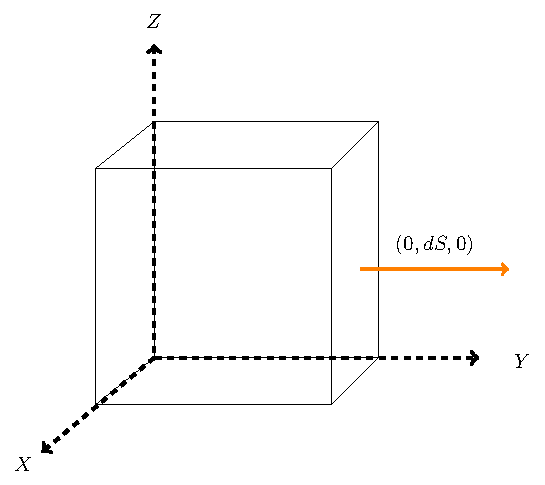
\includegraphics[width=0.5\linewidth]{1_(27-09-2018_electro}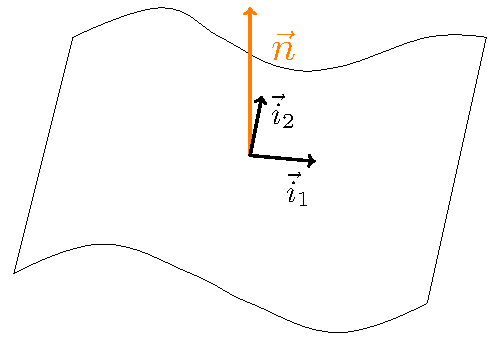
\includegraphics[width=0.5\linewidth]{2_(27-09-2018_electro}
\par\end{center}

Juntando las ecuaciones \vref{eq:IntV a IntV Expandida} y \vref{eq:IntV a int S},
obtenemos:

\begin{equation}
\oiint_{S'}\phi\frac{\partial\psi}{\partial\hat{n}}dS'=\iiint_{V'}\left(\phi\cdot\nabla^{2}\psi+\vec{\nabla}\psi\cdot\vec{\nabla}\phi\right)dV'\label{eq:Id phi}
\end{equation}
Análogamente (repitiendo todo el razonamiento hasta este punto, pero
intercambiando los roles de $\phi$ y $\psi$), llegamos a:

\begin{equation}
\oiint_{S'}\psi\frac{\partial\phi}{\partial\hat{n}}dS'=\iiint_{V'}\left(\psi\cdot\nabla^{2}\phi+\vec{\nabla}\phi\cdot\vec{\nabla}\psi\right)dV'\label{eq:Id psi}
\end{equation}
Hallando la resta de las ecuación \vref{eq:Id psi} y \vref{eq:Id phi},
obtenemos:

\[
\oiint_{S'}\left(\psi\frac{\partial\phi}{\partial\hat{n}}-\phi\frac{\partial\psi}{\partial\hat{n}}\right)dS'=\iiint_{V'}\left(\psi\nabla^{2}\phi-\phi\nabla^{2}\psi\right)dV'
\]
\end{proof}

\subsection{Teorema de Green en física}
\begin{thm}[Teorema de Green en física]
\label{thm:GreenFis}

Supongamos un volumen $V'$ delimitado por la superficie cerrada $S'$.
Además, supongamos que conocemos perfectamente la densidad de carga
$\rho$ dentro de nuestro volumen, pero desconocemos la que hay fuera.
Sin embargo, conocemos el valor de la componente del campo eléctrico
$\vec{E}$ que es perpendicular a la superficie $S'$ en todo punto
de dicha superficie. Además, conocemos el valor del potencial en toda
la superficie $S'$. Entonces, el potencial en cualquier punto de
nuestro volumen $V'$ viene dado por la expresión:
\end{thm}
\[
\phi\left(\vec{R}'\right)=\underbrace{\frac{1}{4\pi\varepsilon_{0}}\iiint_{V'}\frac{\rho\left(\vec{R}'\right)dV'}{r}}_{\begin{matrix}\text{potencial de las cargas}\\
\text{dentro del volumen}
\end{matrix}}+\underbrace{\frac{1}{4\pi}\oiint_{S'}\left(\frac{1}{r}\overbrace{\frac{\partial\phi}{\partial\hat{n}}}^{=-\vec{E}\cdot\hat{n}}-\overbrace{\phi\frac{\partial\left(\frac{1}{r}\right)}{\partial\hat{n}}}^{\begin{matrix}\text{el potencial en}\\
\text{la superficie}\\
\text{(capa dipolar)}
\end{matrix}}\right)dS'}_{\text{lo que sucede fuera del volumen}}
\]

\begin{proof}
Gráficamente, tenemos la siguiente situación:
\begin{center}
\textcolor{green}{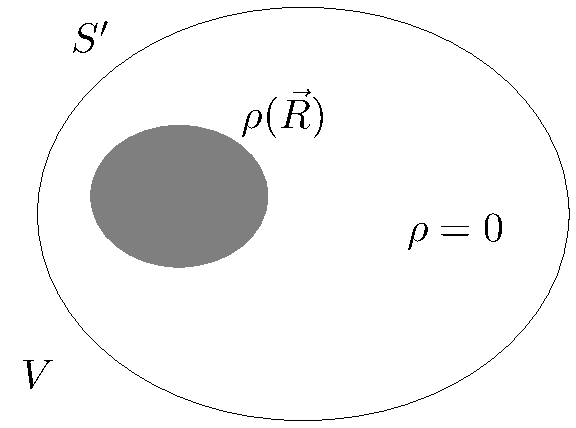
\includegraphics[width=0.55\linewidth]{1_(28-09-2018_electro)}}
\par\end{center}

Tomamos:
\[
\psi:=\frac{1}{r}
\]
y, ahora, por la segunda identidad de Green (ver teorema \vref{thm:Green}),
tenemos:

\[
\iiint_{V'}\left(-\frac{1}{r}\frac{\rho\left(\vec{R}'\right)}{\varepsilon_{0}}-\phi\left(\vec{R}'\right)\underbrace{\nabla^{2}\left(\frac{1}{r}\right)}_{=-4\pi\delta\left(\vec{r}\right)}\right)dV'=\oiint_{S'}\left(\frac{1}{r}\frac{\partial\phi}{\partial\hat{n}}-\phi\frac{\partial\left(\frac{1}{r}\right)}{\partial\hat{n}}\right)dS'
\]
Por la proposición \vref{prop:Lapl 1/r =00003D delta} y recordando
que $\vec{r}=\vec{R}-\vec{R}'$, tenemos que lo anterior es equivalente
a:

\[
-\frac{1}{\varepsilon_{0}}\iiint\frac{\rho\left(\vec{R}'\right)dV'}{r}+\iiint_{V'}\phi\left(\vec{R}'\right)4\pi\delta\left(\vec{R}-\vec{R}'\right)dV'=\oiint_{S'}\left(\frac{1}{r}\frac{\partial\phi}{\partial\hat{n}}-\phi\frac{\partial\left(\frac{1}{r}\right)}{\partial\hat{n}}\right)dS'
\]
Por la propiedad de traslación de la delta (ver proposición \vref{prop:TrasDelta}),
lo anterior es equivalente a:

\[
-\frac{1}{\varepsilon_{0}}\iiint\frac{\rho\left(\vec{R}'\right)dV'}{r}+4\pi\phi\left(\vec{R}\right)=\oiint_{S'}\left(\frac{1}{r}\frac{\partial\phi}{\partial\hat{n}}-\phi\frac{\partial\left(\frac{1}{r}\right)}{\partial\hat{n}}\right)dS'\Leftrightarrow
\]

\[
\phi\left(\vec{R}\right)=\frac{1}{4\pi\varepsilon_{0}}\iiint_{V'}\frac{\rho\left(\vec{R}'\right)dV'}{r}+\frac{1}{4\pi}\oiint_{S'}\left(\frac{1}{r}\frac{\partial\phi}{\partial\hat{n}}-\phi\frac{\partial\left(\frac{1}{r}\right)}{\partial\hat{n}}\right)dS'
\]
\end{proof}
\begin{lem}
\label{lem:Psi}Sean $\Omega$ un abierto en $\mathbb{R}^{3}$ y $\psi:\mathbb{R}^{3}\longrightarrow\mathbb{R}\ni\psi\in C^{2}\left(\mathbb{R}^{3},\mathbb{R}\right)$,
entonces se cumple:

\[
\vec{\nabla}\cdot\left(\psi\vec{\nabla}\psi\right)-\psi\nabla^{2}\psi=\vec{\nabla}\psi\cdot\vec{\nabla}\psi=\left|\vec{\nabla}\psi\right|^{2}
\]
\end{lem}
\begin{proof}[{*}Demostración (No entra)]
 Por la definición de divergencia (ver definición \vref{def:divergencia})
y por la definición de gradiente (ver definición \vref{def:grad}),
tenemos:

\[
\vec{\nabla}\cdot\left(\psi\vec{\nabla}\psi\right)=\left(\frac{\partial}{\partial x},\frac{\partial}{\partial y},\frac{\partial}{\partial z}\right)\cdot\left(\psi\frac{\partial\psi}{\partial x},\psi\frac{\partial\psi}{\partial y},\psi\frac{\partial\psi}{\partial z}\right)=\frac{\partial}{\partial x}\left(\psi\frac{\partial\psi}{\partial x}\right)+\frac{\partial}{\partial y}\left(\psi\frac{\partial\psi}{\partial y}\right)+\frac{\partial}{\partial z}\left(\psi\frac{\partial\psi}{\partial z}\right)=
\]

\[
=\frac{\partial\psi}{\partial x}\frac{\partial\psi}{\partial x}+\psi\frac{\partial^{2}\psi}{\partial x^{2}}+\frac{\partial\psi}{\partial y}\frac{\partial\psi}{\partial y}+\psi\frac{\partial^{2}\psi}{\partial y^{2}}+\frac{\partial\psi}{\partial z}\frac{\partial\psi}{\partial z}+\psi\frac{\partial^{2}\psi}{\partial z^{2}}=
\]

\[
=\left(\frac{\partial\psi}{\partial x}\right)^{2}+\psi\frac{\partial^{2}\psi}{\partial x^{2}}+\left(\frac{\partial\psi}{\partial y}\right)^{2}+\psi\frac{\partial^{2}\psi}{\partial y^{2}}+\left(\frac{\partial\psi}{\partial z}\right)^{2}+\psi\frac{\partial^{2}\psi}{\partial z^{2}}=
\]

\[
=\left(\frac{\partial\psi}{\partial x}\right)^{2}+\left(\frac{\partial\psi}{\partial y}\right)^{2}+\left(\frac{\partial\psi}{\partial z}\right)^{2}+\psi\left(\frac{\partial^{2}\psi}{\partial x^{2}}+\frac{\partial^{2}\psi}{\partial y^{2}}+\frac{\partial^{2}\psi}{\partial z^{2}}\right)=
\]

\[
=\left(\frac{\partial\psi}{\partial x},\frac{\partial\psi}{\partial y},\frac{\partial\psi}{\partial z}\right)\cdot\left(\frac{\partial\psi}{\partial x},\frac{\partial\psi}{\partial y},\frac{\partial\psi}{\partial z}\right)+\psi\nabla^{2}\psi=\vec{\nabla}\psi\cdot\vec{\nabla}\psi+\psi\nabla^{2}\psi
\]

Entonces, claramente:

\[
\vec{\nabla}\cdot\left(\psi\vec{\nabla}\psi\right)-\psi\nabla^{2}\psi=\vec{\nabla}\psi\cdot\vec{\nabla}\psi+\psi\nabla^{2}\psi-\psi\nabla^{2}\psi=\vec{\nabla}\psi\cdot\vec{\nabla}\psi=\left|\vec{\nabla}\psi\right|^{2}
\]
\end{proof}

\subsection{Teorema de unicidad de la solución de la ecuación de Poisson}
\begin{thm}
La solución de la ecuación de Poisson:
\begin{enumerate}
\item (Condición de Dirichlet) es única si conocemos el potencial en la
superficie que limita el volumen estudiado y dicho potencial es constante
a lo largo de ella.
\item (Condición de von Neumann) no es única, pero todas las soluciones
difieren únicamente en una constante si conocemos la componente perpendicular
a la superficie que limita el volumen estudiado en dicha superficie
al completo.
\end{enumerate}
\end{thm}
\begin{proof}
Tenemos:
\begin{center}
\textcolor{green}{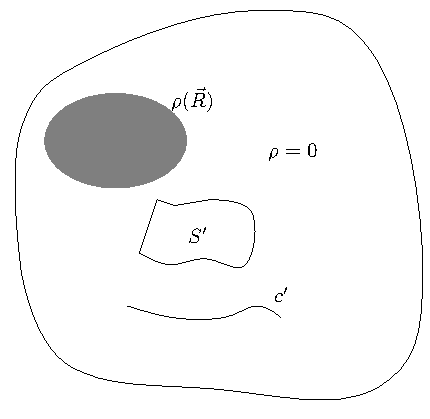
\includegraphics[width=0.55\linewidth]{2_(28-09-2018_electro)}}
\par\end{center}

Partimos de la ecuación de Poisson (ver el teorema \vref{thm:Poisson}):

\[
\nabla^{2}\phi\left(\vec{R}\right)=-\frac{\rho\left(\vec{R}\right)}{\varepsilon_{0}}
\]
Nuestro objetivo ahora es hallar soluciones para esta ecuación diferencial.
Supongamos que $\phi_{1}$ y $\phi_{2}$ son soluciones, entonces
debe ser:

\[
\nabla^{2}\phi_{1}\left(\vec{R}\right)=-\frac{\rho\left(\vec{R}\right)}{\varepsilon_{0}}=\nabla^{2}\phi_{2}\left(\vec{R}\right)
\]
Definamos $\psi:=\phi_{1}-\phi_{2}$. Entonces, como el laplaciano
es un operador lineal:

\[
\nabla^{2}\psi=\nabla^{2}\phi_{1}-\nabla^{2}\phi_{2}=0
\]
\begin{itemize}
\item Justificación de Dirichlet:

Supongamos que conocemos el potencial en la superficie $S$ y que
es constante en ella, entonces:

\[
\phi_{1}\left(\vec{x}\right)=\phi_{2}\left(\vec{x}\right)\;\forall\vec{x}\in S\Rightarrow\psi\left(\vec{x}\right)=\phi_{1}\left(\vec{x}\right)-\phi_{2}\left(\vec{x}\right)=0\;\forall\vec{x}\in S\Rightarrow\oiint_{S}\psi\vec{\nabla}\psi\cdot d\vec{S}=0
\]
Por tanto, por el teorema de la divergencia (ver teorema \vref{thm:Divergencia}):
\[
0=\oiint_{S}\psi\vec{\nabla}\psi\cdot d\vec{S}=\iiint_{V}\vec{\nabla}\cdot\left(\psi\vec{\nabla}\psi\right)dV
\]

Ahora, usando el lema \vref{lem:Psi}:

\[
\iiint_{V}\left[\left|\vec{\nabla}\psi\right|^{2}+\psi\nabla^{2}\psi\right]dV=0
\]

Como era $\psi=0$, debe ser necesariamente $\left|\vec{\nabla}\psi\right|^{2}=0$.
Ahora bien:

\[
\left|\vec{\nabla}\psi\right|^{2}=0\text{ en todo }V\Rightarrow\vec{\nabla}\psi=\vec{0}\text{ en todo }V\Rightarrow\vec{\nabla}\phi_{1}=\vec{\nabla}\phi_{2}\text{ en todo }V\Rightarrow\vec{E}_{1}=\vec{E}_{2}\text{ en todo }V
\]

Además como $\phi_{1}\left(\vec{x}\right)=\phi_{2}\left(\vec{x}\right)\;\forall\vec{x}\in S$,
necesariamente $\phi_{1}=\phi_{2}$ en todo $V$.
\item Justificación de von Neumann:

Si conocemos la componente perpendicular del campo en la superficie,
entonces:

\[
\left[\frac{\partial\phi_{1}}{\partial\hat{n}}\right]_{S}=\left[\frac{\partial\phi_{2}}{\partial\hat{n}}\right]_{S}\Rightarrow\left[\frac{\partial\psi}{\partial\hat{n}}\right]_{S}=0\Rightarrow\vec{\nabla}\psi\cdot d\vec{S}=\vec{0}\Rightarrow\oiint_{S}\vec{\nabla}\psi\cdot d\vec{S}=0
\]

Como $d\vec{S}\neq\vec{0}$, debe ser $\vec{\nabla}\psi=\vec{0}$,
lo cual implica forzosamente: $\vec{\nabla}\phi_{1}=\vec{\nabla}\phi_{2}$
en la superficie. Ahora bien, por el teorema de la divergencia (ver
teorema \vref{thm:Divergencia}):
\[
0=\iint_{S}\vec{\nabla}\psi\cdot d\vec{S}=\iiint_{V}\vec{\nabla}\cdot\vec{\nabla}\psi dV=\iiint_{V}\nabla^{2}\psi dV\Rightarrow\nabla^{2}\psi=0\text{ en todo }V
\]

Por otra parte, también por el teorema de la divergencia (ver teorema
\vref{thm:Divergencia}):
\[
\vec{\nabla}\psi=0\Rightarrow0=\oiint_{S}\psi\vec{\nabla}\psi\cdot d\vec{S}=\iiint_{V}\vec{\nabla}\cdot\left(\psi\vec{\nabla}\psi\right)dV
\]
Por el lema \vref{lem:Psi}, lo anterior es equivalente a:
\[
\iiint_{V}\left[\left|\vec{\nabla}\psi\right|^{2}+\psi\nabla^{2}\psi\right]dV=0
\]

Como era $\nabla^{2}\psi=0$, debe ser necesariamente $\left|\vec{\nabla}\psi\right|^{2}=0$:

\[
\left|\vec{\nabla}\psi\right|^{2}=0\text{ en todo }V\Rightarrow\vec{\nabla}\psi=\vec{0}\text{ en todo }V\Rightarrow\vec{\nabla}\phi_{1}=\vec{\nabla}\phi_{2}\text{ en todo }V\Rightarrow\vec{E}_{1}=\vec{E}_{2}\text{ en todo }V
\]

\end{itemize}
\end{proof}
\begin{example}
Imaginemos:

\begin{center}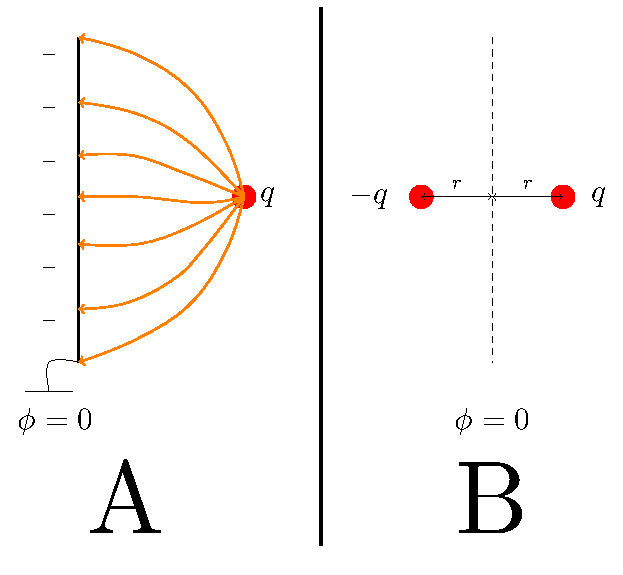
\includegraphics[width=0.6\linewidth]{electromagnetismo_2018_09_28_3}\end{center}

Ambos problemas A y B son equivalentes. La función $\phi$ es la misma
en ambos problemas.
\end{example}

\chapter{Distribuciones de dipolos}

\thispagestyle{newchapter}

Un dipolo es lo siguiente:
\begin{center}
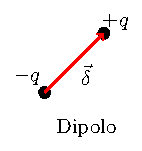
\includegraphics[width=0.4\linewidth]{electromagnetismo_2018_10_02_1}
\par\end{center}

Un cuadrupolo es lo siguiente:
\begin{center}
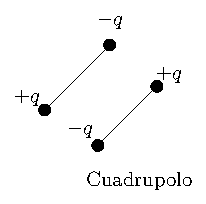
\includegraphics[width=0.4\linewidth]{electromagnetismo_2018_10_02_2}
\par\end{center}

Nótese que ambos se caracterizan porque la carga total es nula. Análogamente,
un octupolo es:
\begin{center}
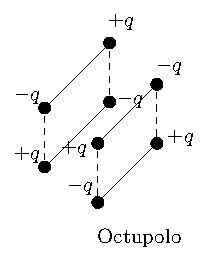
\includegraphics[width=0.4\linewidth]{electromagnetismo_2018_10_02_3}
\par\end{center}

Y, así, sucesivamente.

\section{El dipolo eléctrico. Momento dipolar:}

Nos encontramos ante la siguiente situación:
\begin{center}
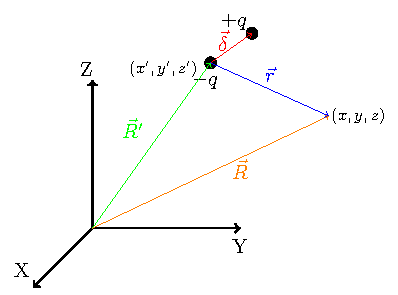
\includegraphics[width=0.6\linewidth]{electromagnetismo_2018_10_02_4}
\par\end{center}
\begin{defn}
\label{def:p Dipolar}Llamamos \textbf{momento dipolar} al vector:

\[
\vec{p}:=q\vec{\delta}
\]
donde $\vec{\delta}$ es el vector que va de la carga negativa a la
positiva.
\end{defn}

\section{Potencial generado por un dipolo}
\begin{prop}
\label{prop:PhiDipolo}El potencial $\phi$ generado por un dipolo
(dos cargas puntuales de signo contrario) cuando $\left|\vec{\delta}\right|\ll\left|\vec{r}\right|$
en un punto $\vec{R}$ es:

\[
\boxed{\phi_{\text{dipolo}}\left(\vec{R}\right)\approx\frac{1}{4\pi\varepsilon_{0}}\frac{\vec{p}\cdot\hat{r}}{r^{2}}}
\]
\end{prop}
\begin{proof}
El potencial generado por el dipolo (dos cargas puntuales de sentido
contrario) en un punto $\vec{R}$ es:

\[
\phi_{\text{dipolo}}\left(\vec{R}\right)=\phi_{+q}^{\vec{R}'+\vec{\delta}}+\phi_{-q}^{\vec{R}'}=\phi_{+q}^{\vec{R}'+\vec{\delta}}-\phi_{+q}^{\vec{R}'}
\]

donde con los superíndices denotamos la posición y con los subíndices
indicamos la carga. Es decir, el potencial que genera el dipolo en
el punto $\vec{R}$ es el que que genera una carga $-q$ en el punto
$\vec{R}'$ más el que genera una carga $q$ en el punto $\vec{R}'+\vec{\delta}$,
pero esto último podemos reescribirlo como el potencial que genera
una carga $q$ en el punto $\vec{R}'+\vec{\delta}$ menos el potencial
generado por una carga $q$ en el punto $\vec{R}'$, pues $\phi_{-q}^{\vec{R}'}=-\phi_{q}^{\vec{R}'}$.

Gráficamente:
\begin{center}
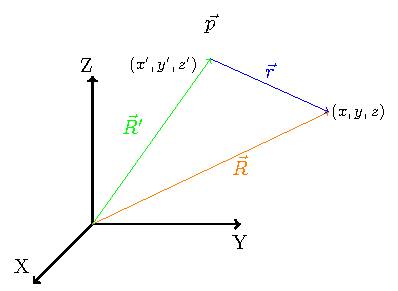
\includegraphics[width=0.6\linewidth]{electromagnetismo_2018_10_02_5}
\par\end{center}

Lo anterior es una diferencia de potencial, luego podemos definir:

\[
\phi_{\text{dipolo}}\left(\vec{R}\right)=\Delta\phi\left(\vec{R}\right):=\phi_{+q}^{\vec{R}'+\vec{\delta}}-\phi_{+q}^{\vec{R}'}
\]
En consecuencia, nuestro problema inicial es equivalente a estudiar
lo que cambiaría el potencial si moviéramos una carga $+q$ del punto
$\vec{R}'$ al punto $\vec{R}'+\vec{\delta}$.

Por otra parte, $\left|\vec{\delta}\right|\ll\left|\vec{r}\right|\Rightarrow\vec{R}'+\vec{\delta}\approx\vec{R}'+{\displaystyle \lim_{\vec{\delta}\rightarrow\vec{0}}\vec{\delta}}$.
Si $\vec{\delta}\rightarrow\vec{0}$, entonces $\Delta\phi\left(\vec{R}\right)\rightarrow\vec{0}$.
Es decir, como $\vec{\delta}$ es muy pequeño respecto a $\vec{R}'$,
podemos aproximar la variación de potencial por un diferencial de
potencial:

\[
\Delta\phi\left(\vec{R}\right)\approx d\phi\left(\vec{R}\right)
\]

Lo que hacemos en el fondo es:

\[
\frac{q}{4\pi\varepsilon_{0}}\left(\frac{\vec{R}-\vec{R}'-\vec{\delta}}{\left|\vec{R}-\vec{R}'-\vec{\delta}\right|^{2}}-\frac{\vec{R}-\vec{R}'}{\left|\vec{R}-\vec{R}'\right|^{2}}\right)\approx\frac{q}{4\pi\varepsilon_{0}}\frac{-\vec{\delta}}{\left|\vec{R}-\vec{R}'\right|^{2}}
\]
Esto nos va a permitir usar conceptos ya conocidos del cálculo. Ahora
bien, si recordamos lo que era el diferencial de una función\footnote{Sean $\Omega$ abierto en $\mathbb{R}^{n}$ y $\begin{matrix}f: & \Omega & \longrightarrow & R\\
 & \left(x_{1},\dots x_{n}\right) &  & f\left(x_{1},\dots,x_{n}\right)
\end{matrix}$. Entonces se define $df$ como $df:={\displaystyle \sum_{i=1}^{n}\frac{\partial f}{\partial x_{i}}dx_{i}}$.}, vemos que claramente:

\begin{equation}
d\phi\left(\vec{R}\right)=\frac{\partial\phi}{\partial x'}dx'+\frac{\partial\phi}{\partial y'}dy'+\frac{\partial\phi}{\partial z'}dz'=\vec{\nabla}'\phi\left(\vec{R}\right)\cdot\vec{\delta}\label{eq:dphi =00003D gradprima}
\end{equation}
donde $\vec{\delta}=\left(dx',dy',dz'\right)$.

Ahora, por la proposición \vref{prop:gradgrad'1/r}:
\[
\vec{\nabla}\left(\frac{1}{r}\right)=-\vec{\nabla}'\left(\frac{1}{r}\right)\Rightarrow\frac{q}{4\pi\varepsilon_{0}}\vec{\nabla}\left(\frac{1}{r}\right)=-\frac{q}{4\pi\varepsilon_{0}}\vec{\nabla}'\left(\frac{1}{r}\right)\Leftrightarrow\vec{\nabla}\left(\frac{q}{4\pi\varepsilon_{0}r}\right)=-\vec{\nabla}'\left(\frac{q}{4\pi\varepsilon_{0}r}\right)
\]
Ahora, por la proposición \vref{prop:PhiPuntual}, lo anterior es
equivalente a:
\[
\vec{\nabla}\phi\left(\vec{R}\right)=-\vec{\nabla}'\phi\left(\vec{R}\right)
\]

De esta forma, retomando la ecuación \vref{eq:dphi =00003D gradprima}
y aplicando la proposición \vref{prop:PhiPuntual}:

\[
d\phi\left(\vec{R}\right)=-\vec{\nabla}\phi\left(\vec{R}\right)\cdot\vec{\delta}=-\frac{q}{4\pi\varepsilon_{0}}\vec{\nabla}\left(\frac{1}{r}\right)
\]
Por la proposición \vref{prop:grad1/r}, tenemos:
\[
d\phi\left(\vec{R}\right)=\frac{q}{4\pi\varepsilon_{0}}\frac{\vec{r}}{r^{3}}\cdot\vec{\delta}=\frac{1}{4\pi\varepsilon_{0}}\frac{\vec{r}\cdot\left(q\vec{\delta}\right)}{r^{3}}
\]
Como el producto escalar es conmutativo y $\vec{p}=q\vec{\delta}$:

\[
d\phi\left(\vec{R}\right)=\frac{1}{4\pi\varepsilon_{0}}\frac{\vec{p}\cdot\vec{r}}{r^{3}}=\frac{1}{4\pi\varepsilon_{0}}\frac{\vec{p}\cdot\hat{r}}{r^{2}}
\]
En consecuencia:

\[
\phi_{\text{dipolo}}\left(\vec{R}\right)\approx d\phi\left(\vec{R}\right)=\frac{1}{4\pi\varepsilon_{0}}\frac{\vec{p}\cdot\hat{r}}{r^{2}}
\]
\end{proof}

\section{Campo que genera un dipolo}
\begin{prop}
\label{prop:EDipolo}El campo eléctrico $\vec{E}$ generado por un
dipolo cuyo momento dipolar satisface $\left|\vec{\delta}\right|\ll\left|\vec{r}\right|$,
puede aproximarse por la expresión:

\[
\boxed{\vec{E}\left(\vec{R}\right)\approx\frac{1}{4\pi\varepsilon_{0}}\frac{3\left(\vec{p}\cdot\vec{r}\right)\vec{r}-r^{2}\vec{p}}{r^{5}}}
\]
\end{prop}
\begin{proof}
Simplemente tenemos que aplicar la definición de potencial eléctrico
(ver definición \vref{def:PhiEl=0000E9ctrico}):

\[
\vec{E}\left(\vec{R}\right)=-\vec{\nabla}\phi\left(\vec{R}\right)
\]
Por la proposición \vref{prop:PhiDipolo}, sabemos:

\[
{\displaystyle \phi_{\text{dipolo}}\left(\vec{R}\right)\approx\frac{1}{4\pi\varepsilon_{0}}\frac{\vec{p}\cdot\vec{r}}{r^{3}}=\frac{1}{4\pi\varepsilon_{0}}\frac{{\displaystyle \sum_{j=x,y,z}p_{j}\left(j-j'\right)}}{\left[\underbrace{\left(x-x'\right)^{2}+\left(y-y'\right)^{2}+\left(z-z'\right)^{2}}_{=r^{2}}\right]^{\frac{3}{2}}}}
\]
Derivando, obtenemos:

\[
\frac{\partial\phi}{\partial x}=\frac{1}{4\pi\varepsilon_{0}}\left(\frac{r^{3}p_{x}-\left[{\displaystyle \sum_{j=x,y,z}}p_{j}\left(j-j'\right)\right]\frac{3}{2}r\cdot2\left(x-x'\right)\cdot1}{r^{6}}\right)=\frac{1}{4\pi\varepsilon_{0}}\left(\frac{p_{x}r^{2}-3\left[{\displaystyle \sum_{j=x,y,z}}p_{j}\left(j-j'\right)\right]\left(x-x'\right)}{r^{5}}\right)=
\]

\[
=\frac{1}{4\pi\varepsilon_{0}}\frac{p_{x}r^{2}-3\vec{p}\cdot\vec{r}\left(x-x'\right)}{r^{5}}
\]
Análogamente:

\[
\frac{\partial\phi}{\partial y}=\frac{1}{4\pi\varepsilon_{0}}\left(\frac{p_{y}r^{2}-3\vec{p}\cdot\vec{r}\left(y-y'\right)}{r^{5}}\right)
\]

\[
\frac{\partial\phi}{\partial z}=\frac{1}{4\pi\varepsilon_{0}}\left(\frac{p_{z}r^{2}-3\vec{p}\cdot\vec{r}\left(z-z'\right)}{r^{5}}\right)
\]

Ahora:

\[
\vec{E}\left(\vec{R}\right)=-\vec{\nabla}\phi\left(\vec{R}\right)=
\]

\[
=\frac{1}{4\pi\varepsilon_{0}}\frac{1}{r^{5}}\left(-p_{x}r^{2}+3\vec{p}\cdot\vec{r}\left(x-x'\right),-p_{y}r^{2}+3\vec{p}\cdot\vec{r}\left(y-y'\right),-p_{z}r^{2}+3\vec{p}\cdot\vec{r}\left(z-z'\right)\right)=
\]

\[
=\frac{1}{4\pi\varepsilon_{0}}\frac{1}{r^{5}}\left[-r^{2}\underbrace{\left(p_{x},p_{y},p_{z}\right)}_{=\vec{p}}+3\vec{p}\cdot\vec{r}\underbrace{\left(x-x',y-y',z-z'\right)}_{=\vec{r}}\right]=
\]

\[
=\frac{1}{4\pi\varepsilon_{0}}\frac{3\left(\vec{p}\cdot\vec{r}\right)\vec{r}-r^{2}\vec{p}}{r^{5}}
\]
\end{proof}
\begin{rem}
Podemos expresar el campo generado por un dipolo como:

\[
\vec{E}=\alpha\vec{r}+\beta\vec{p}
\]

donde $\alpha,\beta\in\mathbb{R}$. Es decir, el vector campo eléctrico
está contenido en el plano formado por los vectores $\vec{r}$ y $\vec{p}$.

\begin{center}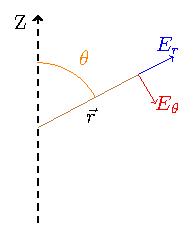
\includegraphics[width=0.45\linewidth]{electromagnetismo_2018_10_02_6}\end{center}

\[
\phi\left(r,\theta\right)=\frac{1}{4\pi\varepsilon_{0}}\frac{pr\cos\theta}{r^{3}}=\frac{1}{4\pi\varepsilon_{0}}\frac{p\cos\theta}{r^{2}}
\]

Si recordamos la expresión del gradiente en coordenadas esféricas,
obtenemos:

\[
\vec{E}=\underbrace{-\frac{\partial\phi}{\partial r}}_{=:E_{r}}\hat{r}\underbrace{-\frac{1}{r}\frac{\partial\phi}{\partial\theta}}_{=:E_{\theta}}\hat{\theta}-\frac{1}{r\sin\theta}\overbrace{\frac{\partial\phi}{\partial\varphi}}^{=0}\hat{\varphi}
\]

pues el campo no depende de la proyección en el plano $XY$.

\[
E_{r}=-\frac{\partial\phi}{\partial r}=\frac{1}{2\pi\varepsilon_{0}}\frac{p\cos\theta}{r^{3}}
\]

\[
E_{\theta}=-\frac{1}{r}\frac{\partial\phi}{\partial\theta}=\frac{1}{r}\frac{1}{4\pi\varepsilon_{0}}\frac{p\sin\theta}{r^{2}}=\frac{1}{4\pi\varepsilon_{0}}\frac{p\sin\theta}{r^{3}}
\]

Por consiguiente:

\[
\vec{E}=\frac{1}{4\pi\varepsilon_{0}}\left(\frac{2p\cos\theta}{r^{3}}\hat{r}+\frac{p\sin\theta}{r^{3}}\hat{\theta}\right)=\frac{p}{4\pi\varepsilon_{0}r^{3}}\left(2\cos\theta\hat{r}+\sin\theta\hat{\theta}\right)
\]

Ahora, podemos hallar las llamadas posiciones de Gauss:

\[
\theta=0\Rightarrow E_{r}=\frac{1}{2\pi\varepsilon_{0}}\frac{p}{r^{3}}\text{ y }E_{\theta}=0
\]

\[
\theta=\frac{\pi}{2}\Rightarrow E_{r}=0\text{ y }E_{\theta}=\frac{1}{4\pi\varepsilon_{0}}\frac{p}{r^{3}}
\]
\end{rem}

\section{$\vec{E}$ y $\phi$ generado por una distribución de dipolos}

Tenemos (como siempre):
\begin{center}
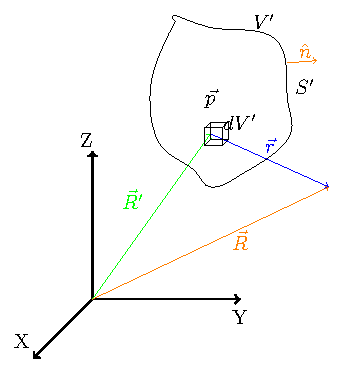
\includegraphics[width=0.55\linewidth]{electromagnetismo_2018_10_02_7}
\par\end{center}
\begin{defn}
Definimos el \textbf{momento dipolar total} como la suma de los momentos
dipolares de todos los dipolos involucrados:

\[
\vec{p}:=\sum_{i=1}^{n}\vec{p}_{i}
\]
\end{defn}
\begin{rem}
Como es usual en física, si el número de partículas es muy alto, podemos
aproximar la suma finita por una integral, de manera que:

\[
\vec{p}\approx\iiint_{V'}d\vec{p}
\]
\end{rem}
\begin{defn}
\label{def:P}Llamamos \textbf{vector densidad de polarización} $\vec{P}$
al vector que describe:

\[
\vec{P}\left(\vec{R}'\right):=\frac{d\vec{p}}{dV'}
\]
siendo:

\[
\left[\vec{P}\right]=\frac{\text{C}\text{m}}{\text{m}^{3}}=\frac{\text{C}}{\text{m}^{2}}
\]
\end{defn}
\begin{cor}
De la definición anterior deducimos fácilmente:

\[
d\vec{p}=\vec{P}\left(\vec{R}'\right)dV'
\]
\end{cor}
\begin{defn}
\label{def:dCargaEquivalentes}Llamamos \textbf{densidad de carga
equivalente} \textbf{volumétrica} o \textbf{densidad de Poisson volumétrica}
a:
\[
\rho_{b}:=-\vec{\nabla}'\cdot\vec{P}\left(\vec{R}'\right)
\]
Análogamente, llamamos \textbf{densidad de carga equivalente superficial}
o \textbf{densidad de Poisson superficial} a:
\[
\sigma_{b}:=\vec{P}\left(\vec{R}'\right)\cdot\hat{n}
\]
donde la $b$ viene por el inglés \textit{bound.}
\end{defn}
\begin{lem}
\label{lem:divEscVec}Sean $\Omega$ y $\Xi$ abiertos de $\mathbb{R}^{n}$
y sen $\varphi:\Omega\subset\mathbb{R}^{n}\rightarrow\mathbb{R}$
una función escalar y $\vec{A}:\Xi\subset\mathbb{R}^{n}\rightarrow\mathbb{R}^{n}$
una función vectorial, diferenciables en sus respectivos dominios,
entonces, para todo $\vec{R}\in\Omega\cap\Xi$, se da:

\[
\vec{\nabla}'\cdot\left(\varphi\vec{A}\right)=\varphi\vec{\nabla}'\cdot\vec{A}+\vec{A}\cdot\vec{\nabla}'\varphi
\]
\end{lem}
\begin{proof}[{*}Demostración (No entra)]

Sea $\vec{A}=\left(A_{1},\dots,A_{n}\right)$:

\[
\vec{\nabla}'\cdot\left(\varphi\vec{A}\right)=\left(\frac{\partial}{\partial x'_{1}},\dots,\frac{\partial}{\partial x'_{n}}\right)\cdot\left(\varphi A_{1},\dots,\varphi A_{n}\right)=\sum_{i=1}^{n}\frac{\partial}{\partial x'_{i}}\left(\varphi A_{i}\right)=
\]

\[
=\sum_{i=1}^{n}\left[\frac{\partial\varphi}{\partial x'_{i}}A_{i}+\varphi\frac{\partial A_{i}}{\partial x'_{i}}\right]=\varphi\sum_{i=1}^{n}\frac{\partial}{\partial x'_{i}}\left(A_{i}\right)+\sum_{i=1}^{n}A_{i}\cdot\frac{\partial\varphi}{\partial x'_{i}}=
\]

\[
=\varphi\underbrace{\left(\frac{\partial}{\partial x'_{1}},\dots,\frac{\partial}{\partial x'_{n}}\right)}_{=\vec{\nabla}'}\cdot\underbrace{\left(A_{1},\dots,A_{n}\right)}_{=\vec{A}}+\underbrace{\left(A_{1},\dots,A_{n}\right)}_{=\vec{A}}\cdot\underbrace{\left(\frac{\partial\varphi}{\partial x'_{1}},\dots,\frac{\partial\varphi}{\partial x'_{n}}\right)}_{=\vec{\nabla}'\varphi}=
\]

\[
=\varphi\vec{\nabla}'\cdot\vec{A}+\vec{A}\cdot\vec{\nabla}'\varphi
\]
\end{proof}
\begin{prop}
\label{prop:PhiEDistDipolo}Sea una distribución de dipolos que ocupa
un volumen $V'$ y sea $S'$ la superficie cerrada que engloba dicho
volumen, entonces el potencial y el campo eléctrico generado por dicha
distribución de dipolos pueden expresarse como:
\begin{enumerate}
\item 
\[
\boxed{\phi\left(\vec{R}\right)=\frac{1}{4\pi\varepsilon_{0}}\left[\oiint_{S'}\frac{\sigma_{b}}{r}dS'+\iiint_{V'}\frac{\rho_{b}}{r}dV'\right]}
\]
\item 
\[
\boxed{\vec{E}\left(\vec{R}\right)=\frac{1}{4\pi\varepsilon_{0}}\left[\oiint_{S'}\frac{\sigma_{b}\vec{r}}{r^{3}}dS'+\iiint_{V'}\frac{\rho_{b}\vec{r}}{r^{3}}dV'\right]}
\]
\end{enumerate}
\end{prop}
\begin{proof}
Tomando la diferencial a ambos lados en la proposición \vref{prop:PhiDipolo},
obtenemos: 

\[
d\phi\left(\vec{R}\right)=\frac{1}{4\pi\varepsilon_{0}}\frac{d\vec{p}}{r^{3}}\cdot\vec{r}
\]
Aplicando la definición \vref{def:P}, podemos expresar el potencial
como:

\[
\phi\left(\vec{R}\right)=\frac{1}{4\pi\varepsilon_{0}}\iiint_{V'}\frac{d\vec{p}\cdot\vec{r}}{r^{3}}=\frac{1}{4\pi\varepsilon_{0}}\iiint_{V'}\frac{\vec{P}\left(\vec{R}'\right)\cdot\vec{r}}{r^{3}}dV'=\frac{1}{4\pi\varepsilon_{0}}\iiint_{V'}\vec{P}\left(\vec{R}'\right)\cdot\frac{\vec{r}}{r^{3}}dV'
\]
Usando la proposición\vref{prop:gradgrad'1/r}, reescribirmos la expresión
anterior como:
\begin{equation}
\phi\left(\vec{R}\right)=\frac{1}{4\pi\varepsilon_{0}}\iiint_{V'}\vec{P}\left(\vec{R}\right)\cdot\vec{\nabla}'\left(\frac{1}{r}\right)\label{eq:P=00005CcdotgradPrima1/r}
\end{equation}

Por otra parte, haciendo uso del lema \vref{lem:divEscVec} y tomando
${\displaystyle \phi=\frac{1}{r}}$ y $\vec{A}=\vec{P}\left(\vec{R}\right)$,
llegamos a:

\[
\vec{\nabla}'\left(\frac{\vec{P}\left(\vec{R}'\right)}{r}\right)=\frac{\vec{\nabla}'\vec{P}\left(\vec{R}'\right)}{r}+\vec{P}\left(\vec{R}'\right)\cdot\vec{\nabla}'\left(\frac{1}{r}\right)\Leftrightarrow
\]

\[
\Leftrightarrow\vec{\nabla}'\left(\frac{\vec{P}\left(\vec{R}'\right)}{r}\right)-\frac{\vec{\nabla}'\vec{P}\left(\vec{R}'\right)}{r}=\vec{P}\left(\vec{R}'\right)\cdot\vec{\nabla}'\left(\frac{1}{r}\right)
\]

En consecuencia, podemos sustituir lo anterior en la ecuación \vref{eq:P=00005CcdotgradPrima1/r},
obteniendo:

\[
\phi\left(\vec{R}\right)=\frac{1}{4\pi\varepsilon_{0}}\left[\iiint_{V'}\vec{\nabla}'\left(\frac{\vec{P}\left(\vec{R}'\right)}{r}\right)dV'+\iiint_{V'}\left(\frac{-\vec{\nabla}'\vec{P}\left(\vec{R}'\right)}{r}\right)dV'\right]
\]
Por el teorema de la divergencia (\vref{thm:Divergencia}):

\[
\phi\left(\vec{R}\right)=\frac{1}{4\pi\varepsilon_{0}}\oiint_{S'}\frac{\vec{P}\left(\vec{R}'\right)\cdot\hat{n}}{r}dS'+\frac{1}{4\pi\varepsilon_{0}}\iiint_{V'}-\frac{\vec{\nabla}'\vec{P}\left(\vec{R}'\right)}{r}dV'
\]
donde $d\vec{S}'=\hat{n}dS'$ y $\hat{n}$ es el vector unitario normal
a la superficie $S'$. Usando las definiciones \vref{def:dCargaEquivalentes},
el potencial queda:

\[
\phi\left(\vec{R}\right)=\frac{1}{4\pi\varepsilon_{0}}\left[\oiint_{S'}\frac{\sigma_{b}}{r}dS'+\iiint_{V'}\frac{\rho_{b}}{r}dV'\right]
\]

Hallamos el campo eléctrico (aplicamos $\vec{E}=-\vec{\nabla}\phi$,
ver definición \vref{def:PhiEl=0000E9ctrico}) :
\[
\vec{E}=-\vec{\nabla}\phi=-\frac{1}{4\pi\varepsilon_{0}}\left[\oiint_{S'}\sigma_{b}\vec{\nabla}\left(\frac{1}{r}\right)dS'+\iiint_{V'}\rho_{b}\vec{\nabla}\left(\frac{1}{r}\right)dV'\right]
\]
pues la divergencia y la integral conmutan al ser la integral a las
coordenadas primadas y la divergencia a las coordenadas sin primar.
Por la proposición \vref{prop:grad1/r}, la expresión anterior queda:

\[
\vec{E}\left(\vec{R}\right)=\frac{1}{4\pi\varepsilon_{0}}\left[\oiint_{S'}\frac{\sigma_{b}\vec{r}}{r^{3}}dS'+\iiint_{V'}\frac{\rho_{b}\vec{r}}{r^{3}}dV'\right]
\]
\end{proof}
\begin{example}
Tenemos:
\begin{center}
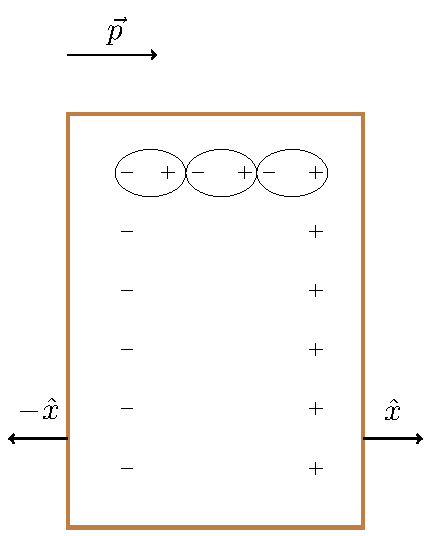
\includegraphics[width=0.4\linewidth]{electro_ausente1}
\par\end{center}

En el interior los dipolos se anulan y no hay $\rho_{b}$, pero lo
habría si el volumen fuese irregular (con, por ejemplo, huecos (<<burbujas>>)
en su interior).

La carga ligada sería:

\[
Q_{b}=\iiint_{V'}-\vec{\nabla}'\vec{P}\left(\vec{R}'\right)dV'+\oiint_{S'}\vec{P}d\vec{S}'
\]
Por el teorema de la divergencia (ver teorema \vref{thm:Divergencia}),
lo anterior es equivalente a:
\[
Q_{b}=-\oiint_{S'}\vec{P}d\vec{S}'+\oiint_{S'}\vec{P}d\vec{S}'=0
\]

Por otra parte:

\[
0=Q_{b}=\iiint_{V'}\rho_{b}dV'+\oiint_{S'}\sigma_{b}dS'
\]
\end{example}
%
\begin{example}[<<El electrete>>]
Tenemos:

\begin{center}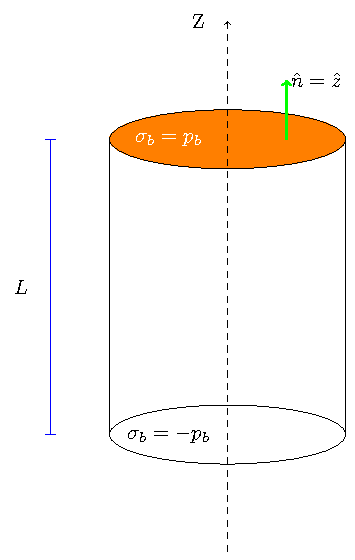
\includegraphics[width=0.35\linewidth]{electro_ausente2}\end{center}
\[
\vec{P}=P_{0}\hat{z}
\]

\[
\rho_{b}=-\vec{\nabla}\cdot\vec{P}=0+0+\underbrace{\frac{\partial P_{z}}{\partial z}}_{=0}=0
\]

\[
\sigma_{b}=\left\{ \begin{matrix}\text{tapa superior:} &  & \vec{P}\cdot\hat{n}=P_{0}\\
\text{superficie lateral:} &  & P_{0}\hat{z}\cdot\hat{r}=0\\
\text{tapa inferior:} &  & P_{0}\hat{z}\cdot\left(-\hat{z}\right)=-P_{0}
\end{matrix}\right.
\]

Hemos reducido al vacío; es decir: resulta que tener un cilindro polarizado
como éste es equivalente a tener dos discos.
\end{example}

\chapter{Desarrollo multipolar: potenciales y momentos}

\thispagestyle{newchapter}

\section{Una primera introducción}

Veamos un ejemplo para comprender lo que queremos hacer:
\begin{center}
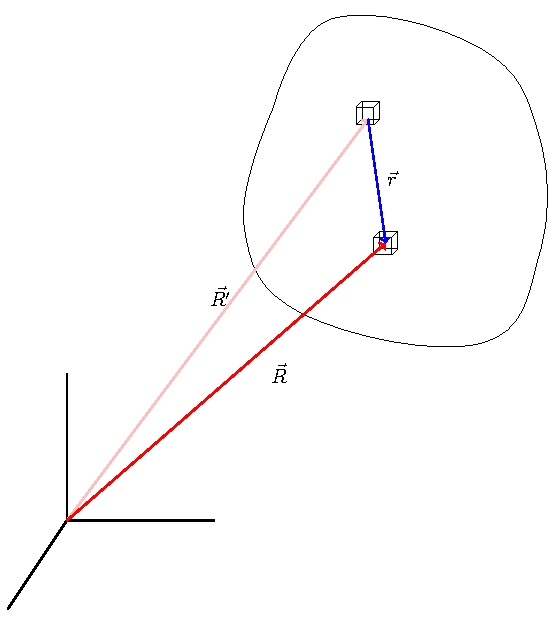
\includegraphics[width=0.55\linewidth]{electromagnetismo_2018_10_03_1}
\par\end{center}

Nuestro objetivo va a ser reemplazar ${\displaystyle \frac{1}{r}}$
por ${\displaystyle \frac{1}{R}}$, donde $R$ representa la distancia
a nuestro origen de coordenadas esféricas. Es decir conseguir:

\[
\frac{1}{r}\approxeq\frac{1}{R}+\dots
\]

\[
\phi\left(\vec{R}\right)=\frac{1}{4\pi\varepsilon_{0}}\frac{q}{r}
\]
donde:

\[
r=\sqrt{\left(x-0\right)^{2}+\left(y-0\right)^{2}+\left(z-\frac{a}{2}\right)^{2}}
\]

\begin{center}
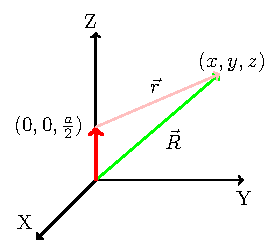
\includegraphics[width=0.55\linewidth]{electromagnetismo_2018_10_03_2}
\par\end{center}

Como siempre nuestra intención es obtener una expresión para el potencial.

\section{Ejemplo: la carga puntual}
\begin{defn}
\label{def:PolinomiosLegendre}Llamamos \textbf{polinomio $n$-ésimo
de Legendre} al polinomio:

\[
P_{n}\left(x\right):=\frac{1}{2^{n}n!}\frac{d^{n}}{dx^{n}}\left[\left(x^{2}-1\right)^{2}\right]
\]
\end{defn}
\begin{example}[La carga puntual]
Imaginemos:
\begin{center}
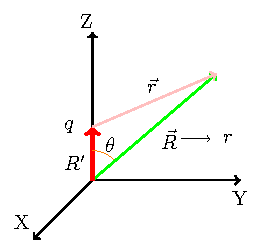
\includegraphics[width=0.55\linewidth]{electromagnetismo_2018_10_03_3}
\par\end{center}

Claramente:

\[
\vec{R}'=a\cdot\hat{z}=\left(0,0,a\right)
\]

\[
\phi\left(\vec{R}\right)=\frac{1}{4\pi\varepsilon_{0}}\frac{q}{r}
\]
Aplicando el teorema del coseno, obtenemos:

\[
r^{2}=a^{2}+R^{2}-2aR\cos\theta
\]
En consecuencia:

\[
\phi\left(\vec{R}\right)=\frac{1}{4\pi\varepsilon_{0}}\frac{q}{\sqrt{R^{2}+a^{2}-2aR\cos\theta}}
\]

Cambiando la notación a $r\equiv R$, obtenemos:

\[
\phi\left(\vec{r}\right)=\frac{q}{4\pi\varepsilon_{0}}\frac{1}{\sqrt{r^{2}+a^{2}-2ar\cos\theta}}
\]
donde $r$ es la distancia al origen en coordenadas esféricas. Estudiemos:

\[
\frac{1}{\sqrt{r^{2}+a^{2}-2ar\cos\theta}}=\frac{1}{r\sqrt{1+\left(\frac{a}{r}\right)^{2}-2\left(\frac{a}{r}\right)\cos\theta}}=\frac{1}{r}\left[1+\left(\frac{a}{r}\right)^{2}-2\left(\frac{a}{r}\right)\cos\theta\right]^{-\frac{1}{2}}
\]

Por otra parte, conocemos el siguiente desarrollo en serie de Taylor:

\[
\left[1+x\right]^{-\frac{1}{2}}=1-\frac{1}{2}x+\frac{1\cdot3}{2\cdot4}x^{2}-\frac{1\cdot3\cdot5}{2\cdot4\cdot6}x^{3}+\dots\;\forall-1\le x\le1
\]
Si aplicamos el desarrollo descrito, llegamos a:

\[
\frac{1}{r}\left[1+\left(\frac{a}{r}\right)^{2}-2\left(\frac{a}{r}\right)\cos\theta\right]^{-\frac{1}{2}}=
\]

\[
=\frac{1}{r}\left[1-\frac{1}{2}\left(\left(\frac{a}{r}\right)^{2}-2\frac{a}{r}\cos\theta\right)+\frac{3}{8}\left(\left(\frac{a}{r}\right)^{2}-\frac{a}{r}\cos\theta\right)^{2}+\dots\right]=
\]
\[
=\frac{1}{r}\left[1-\frac{1}{2}\left(\left(\frac{a}{r}\right)^{2}-2\frac{a}{r}\cos\theta\right)+\frac{3}{8}\left(\left(\frac{a}{r}\right)^{4}+4\left(\frac{a}{r}\right)^{2}\cos^{2}\theta-2\left(\frac{a}{r}\right)^{3}\cos\theta\right)+\dots\right]=
\]

\[
=\frac{1}{r}\left[1+\frac{a}{r}\cos\theta+\left(\frac{3}{2}\cos^{2}\theta-\frac{1}{2}\right)\left(\frac{a}{r}\right)^{2}+\dots\right]
\]
De esta forma:

\[
\phi\left(r\right)=\frac{q}{4\pi\varepsilon_{0}r}\left[1+\frac{a}{r}\cos\theta+\frac{3\cos^{2}\theta-1}{2}\left(\frac{a}{r}\right)^{2}+\dots\right]
\]
Podemos ver que justo las funciones que acompañan a $\left(\frac{a}{r}\right)^{i}$
son justo $P_{i}\left(\cos\theta\right)$ donde con $P_{i}$ denotamos
los polinomios de Legendre (ver la definición \vref{def:PolinomiosLegendre}).
Consecuentemente:

\[
\phi\left(r\right)=\frac{q}{4\pi\varepsilon_{0}}\left[P_{0}\left(\cos\theta\right)+\frac{a}{r}P_{1}\left(\cos\theta\right)+\left(\frac{a}{r}\right)^{2}P_{2}\left(\cos\theta\right)+\left(\frac{a}{r}\right)^{3}P_{3}\left(\cos\theta\right)+\dots\right]=
\]

\[
=\frac{1}{4\pi\varepsilon_{0}}\frac{q}{r}\sum_{l=0}^{\infty}\left(\frac{a}{r}\right)^{l}P_{l}\left(\cos\theta\right)
\]
\end{example}
\begin{rem}
Por la expresión anterior, podemos ver que tener una carga a una distancia
$a$ es equivalente a tener una carga puntual en el centro de coordenadas
más un dipolo, más un cuadrupolo, etc.
\end{rem}
%
\begin{rem}
Podemos expresar la densidad de carga cuando sólo tenemos una carga
puntual en el origen como:

\[
\rho\left(\vec{R}\right)=\underbrace{\delta\left(x\right)\delta\left(y\right)\delta\left(z\right)}_{=\delta\left(x,y,z\right)}q
\]

Como ya sabemos:

\[
Q_{T}=\iiint_{V}\rho\left(\vec{R}\right)dV=\iiint_{V}q\delta\left(x,y,z\right)dV
\]

por la propiedad de traslación de la delta (proposición \vref{prop:TrasDelta})
la integral anterior valdrá $q$ si la carga está contenida en $V$
y 0 en caso contrario.
\end{rem}

\section{Ejemplo: $n$ cargas puntuales alineadas}
\begin{example}[$n$ cargas puntuales alineadas]
Tenemos:
\begin{center}
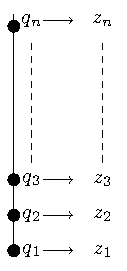
\includegraphics[width=0.2\linewidth]{electromagnetismo_2018_10_03_4}
\par\end{center}

En este caso, podríamos expresar la densidad de carga como:

\[
\rho\left(\vec{R}\right)=\sum_{i=1}^{n}q_{i}\delta\left(x,y,z-z_{i}\right)
\]

De hecho, podemos definir una densidad lineal:

\[
\lambda\left(z'\right)=\sum_{i=1}^{n}q_{i}\delta\left(z-z_{i}\right)
\]
\end{example}

\section{Distribución axial}
\begin{defn}
Llamamos \textbf{momento dipolar axial de orden} $l$ \textbf{a lo
largo del eje} $z$ a:

\[
M_{l}:=\int_{-\infty}^{\infty}\lambda\left(z'\right)\cdot\left(z'\right)^{l}dz'
\]
\end{defn}
\begin{example}[Distribución axial]
~
\begin{center}
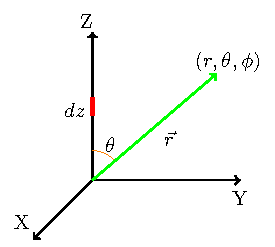
\includegraphics[width=0.55\linewidth]{electromagnetismo_2018_10_05_1}
\par\end{center}

Anteriormente, hemos obtenido:

\[
\phi\left(r,\theta\right)=\frac{1}{4\pi\varepsilon_{0}}\frac{q}{r}\sum_{l=0}^{\infty}\left(\frac{a}{r}\right)^{l}P_{l}\left(\cos\theta\right)
\]
Si la carga está en el eje Z, podemos escribir lo anterior como:

\[
\phi\left(r,\theta\right)=\frac{1}{4\pi\varepsilon_{0}}\frac{q}{r}\sum_{l=0}^{\infty}\left(\frac{z'}{r}\right)^{l}P_{l}\left(\cos\theta\right)
\]
Si ahora tenemos varias cargas alineadas en el eje Z, debe ser:

\[
d\phi\left(r,\theta\right)=\frac{1}{4\pi\varepsilon_{0}}\frac{\lambda\left(z'\right)}{r}\sum_{l=0}^{\infty}\left(\frac{z'}{r}\right)^{l}P_{l}\left(\cos\theta\right)dz'
\]

En consecuencia:

\[
\phi\left(r,\theta\right)=\int_{-\infty}^{\infty}\frac{1}{4\pi\varepsilon_{0}}\frac{\lambda\left(z'\right)}{r}\sum_{l=0}^{\infty}\left(\frac{z'}{r}\right)^{l}P_{l}\left(\cos\theta\right)dz'=
\]

\[
=\frac{1}{4\pi\varepsilon_{0}}\sum_{l=0}^{\infty}\int_{-\infty}^{\infty}\frac{\lambda\left(z'\right)\cdot\left(z'\right)^{l}P_{l}\left(\cos\theta\right)}{r^{l+1}}dz'=
\]

\[
=\frac{1}{4\pi\varepsilon_{0}}\sum_{l=0}^{\infty}\frac{P_{l}\left(\cos\theta\right)}{r^{l+1}}\underbrace{\int_{-\infty}^{\infty}\lambda\left(z'\right)\cdot\left(z'\right)^{l}dz'}_{\begin{matrix}\text{momento dipolar}\\
\text{axial de orden }l\\
=:M_{l}
\end{matrix}}=
\]

\[
=\frac{1}{4\pi\varepsilon_{0}}\sum_{l=0}^{\infty}\frac{M_{l}P_{l}\left(\cos\theta\right)}{r^{l+1}}
\]

Por tanto:

\begin{equation}
\phi\left(r,\theta\right)=\frac{1}{4\pi\varepsilon_{0}}\sum_{l=0}^{\infty}\frac{M_{l}P_{l}\left(\cos\theta\right)}{r^{l+1}}\label{eq:ejAx}
\end{equation}
\end{example}

\section{Ejemplo: tres cargas puntuales alineadas en el eje Z}
\begin{example}[tres cargas puntuales alineadas en el eje Z]
\label{exa:3cargasEjeZ}~
\begin{center}
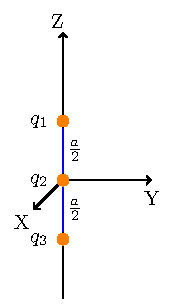
\includegraphics[width=0.25\linewidth]{electromagnetismo_2018_10_05_2}
\par\end{center}

La densidad de carga lineal la podemos expresar como:

\[
\lambda\left(z'\right)=q_{1}\delta\left(z'-\frac{a}{2}\right)+q_{2}\delta\left(z'\right)+q_{3}\delta\left(z'+\frac{a}{2}\right)
\]

\[
M_{0}=\int_{-\infty}^{\infty}\lambda\left(z'\right)\cdot1\cdot dz'=q_{1}+q_{2}+q_{3}=Q_{T}
\]

\[
M_{1}=\int_{-\infty}^{\infty}\lambda\left(z'\right)z'dz'=q_{1}\frac{a}{2}+q_{2}\cdot0-q_{3}\frac{a}{2}
\]

\[
M_{2}=\int_{-\infty}^{\infty}\lambda\left(z'\right)\cdot\left(z'\right)^{2}dz'=q_{1}\left(\frac{a}{2}\right)^{2}+q_{2}\cdot0^{2}+q_{3}\left(-\frac{a}{2}\right)^{2}=\left(q_{1}+q_{3}\right)\left(\frac{a}{2}\right)^{2}
\]

En general:

\[
\left\{ \begin{matrix}M_{l}=\left(q_{1}-q_{3}\right)\left(\frac{a}{2}\right)^{l} & \text{ si } & l\text{ es impar}\\
M_{l}=\left(q_{1}+q_{3}\right)\left(\frac{a}{2}\right)^{l} & \text{ si } & l\text{ es par}
\end{matrix}\right.
\]
\end{example}
%
\begin{example}[el dipolo]

Usando el ejemplo anterior, tomemos $q=q_{1}=-q_{3}$ y $q_{2}=0$.
En este caso:

\[
\begin{matrix}M_{0}=0 &  & M_{1}=q\cdot a &  & M_{2}=0 &  & M_{3}=2a\left(\frac{a}{2}\right)^{3} &  & M_{4}=0\end{matrix}
\]

Para un $l$ cualquiera, $M_{l}$ únicamente será distinto de cero
para los $l$ impares. Obtenemos, al sustituir en \vref{eq:ejAx},
el siguiente potencial:

\[
\phi\left(r,\theta\right)=\frac{1}{4\pi\varepsilon_{0}}\left[0+\frac{q\cdot a\cos\theta}{r^{2}}+0+\frac{q}{r^{4}}\frac{a^{3}\left(5-\cos^{3}\theta-3\cos\theta\right)}{8}+\dots\right]
\]
\end{example}
%
\begin{example}[el cuadrupolo]

Usando el ejemplo \vref{exa:3cargasEjeZ} con los valores $q=q_{3}=q$
y $q_{2}=-2q$, llegamos a:

\[
\begin{matrix}M_{0}=0 &  & M_{1}=0 &  & M_{2}=2q\frac{a^{2}}{4} &  & M_{3}=0\end{matrix}
\]

En general:

\[
\left\{ \begin{matrix}M_{l}=0 & \text{ si } & l\text{ es impar}\\
M_{l}=M_{l}=2q\left(\frac{a}{2}\right)^{l} & \text{ si } & l\text{ es par}
\end{matrix}\right.
\]

De esta forma, sustituyendo en \vref{eq:ejAx}, llegamos a:

\[
\phi\left(r,\theta\right)=\frac{1}{4\pi\varepsilon_{0}}\left[0+0+\frac{qa^{2}}{2}\frac{P_{2}\left(\cos\theta\right)}{r^{3}}+0+\frac{qa^{4}}{8}\frac{P_{4}\left(\cos\theta\right)}{r^{5}}+\dots\right]
\]
\end{example}

\section{Caso general}
\begin{prop}
\label{prop:DesarrolloMultipolarQPrima}El desarrollo multipolar del
potencial eléctrico generado por una distribución de carga cualquiera
es:

\[
\phi\left(\vec{R}\right)=\frac{1}{4\pi\varepsilon_{0}}\left[\frac{q}{R}+\frac{\vec{p}\cdot\vec{R}}{R^{3}}+\frac{1}{2}\sum_{i=1}^{3}\sum_{j=1}^{3}\frac{3x_{i}x_{j}-\delta_{ij}R^{2}}{R^{5}}Q'_{ij}+\dots\right]
\]
donde $q$ representa la carga, $\vec{p}=\iiint_{V'}\rho\left(\vec{R}'\right)\vec{R}'dV'$
y $Q'_{ij}=\iiint_{V'}x'_{i}x_{j}'\rho\left(\vec{R}'\right)dV'$.
\end{prop}
\begin{proof}
Tenemos:
\begin{center}
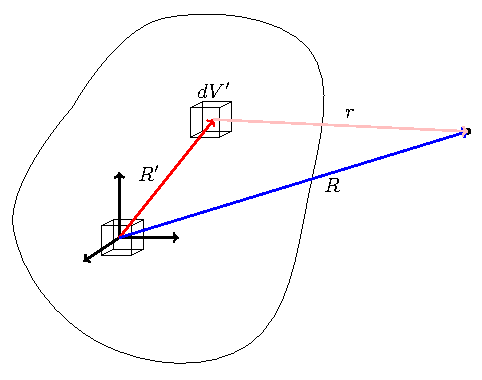
\includegraphics[width=0.6\linewidth]{electromagnetismo_2018_10_09_1}
\par\end{center}

Sabemos:

\[
\phi\left(\vec{R}\right)=\frac{1}{4\pi\varepsilon_{0}}\iiint_{V'}\frac{\rho\left(\vec{R}'\right)}{r}dV'
\]

\[
\vec{r}=\left(x-x',y-y',z-z'\right)
\]

\[
r=\sqrt{\left(x-x'\right)^{2}+\left(y-y'\right)^{2}+\left(z-z'\right)^{2}}
\]
Vamos a hacer el desarrollo en serie de Taylor en torno al punto que
cumple $R'=0$:

\[
\frac{1}{r}=\left[\frac{1}{r}\right]_{R'=0}+\sum_{i=1}^{3}\left[\frac{\partial\left(\frac{1}{r}\right)}{\partial x'_{i}}\right]_{R'=0}x'_{i}+\frac{1}{2}\sum_{i=1}^{3}\sum_{j=1}^{3}\left[\frac{\partial^{2}\left(\frac{1}{r}\right)}{\partial x'_{i}\partial x'_{j}}\right]_{R'=0}x'_{i}x'_{j}+\dots=
\]
\[
=\frac{1}{r}=\left[\frac{1}{r}\right]_{R'=0}+\left[\vec{\nabla}'\left(\frac{1}{r}\right)\right]_{R'=0}\cdot\vec{R}'+\frac{1}{2}\vec{R}'\left[H\left(\frac{1}{r}\right)\right]_{R'=0}\vec{R}'+\dots
\]
donde $H$ es la matriz hessiana.

Recordando ${\displaystyle \frac{\partial\left(\frac{1}{r}\right)}{\partial x_{i}}=-\frac{\partial\left(\frac{1}{r}\right)}{\partial x'_{i}}\;\forall i=1,2,3}$,
podemos expresar lo anterior como:

\[
\frac{1}{r}=\left[\frac{1}{r}\right]_{R'=0}-\sum_{i=1}^{3}\left[\frac{\partial\left(\frac{1}{r}\right)}{\partial x{}_{i}}\right]_{R'=0}x'_{i}+\frac{1}{2}\sum_{i=1}^{3}\sum_{j=1}^{3}\left[\frac{\partial^{2}\left(\frac{1}{r}\right)}{\partial x{}_{i}\partial x_{j}}\right]_{R'=0}x'_{i}x'_{j}+\dots
\]
Ahora:

\[
\frac{\partial\left(\frac{1}{r}\right)}{\partial x_{i}}=\frac{\partial\left(\frac{1}{\left[\left(x-x'\right)^{2}+\left(y-y'\right)^{2}+\left(z-z'\right)^{2}\right]^{\frac{1}{2}}}\right)}{\partial x_{i}}=\frac{-\left(x_{i}-x'_{i}\right)}{r^{3}}
\]

\[
\frac{\partial^{2}\left(\frac{1}{r}\right)}{\partial x_{i}^{2}}=\frac{-r^{3}+\left(x_{i}-x'_{i}\right)3\frac{1}{2}r\left(x_{i}-x'_{i}\right)2}{r^{6}}=\frac{-r^{2}+3\left(x_{i}-x'_{i}\right)^{2}}{r^{5}}
\]

\[
\frac{\partial^{2}\left(\frac{1}{r}\right)}{\partial x_{i}\partial x_{j}}=\frac{\left(x_{i}-x'_{i}\right)3r^{2}\frac{1}{2}\frac{1}{r}2\left(x_{j}-x'_{j}\right)}{r^{6}}=\frac{3\left(x_{i}-x'_{i}\right)\left(x_{j}-x'_{j}\right)}{r^{5}}
\]
En consecuencia:

\[
\left[\frac{\partial\left(\frac{1}{r}\right)}{\partial x_{i}}\right]_{R'=0}=\left[\frac{-\left(x_{i}-x'_{i}\right)}{r^{3}}\right]_{R'=0}=\frac{-x_{i}}{R^{3}}
\]

\[
\left[\frac{\partial^{2}\left(\frac{1}{r}\right)}{\partial x_{i}^{2}}\right]_{R'=0}=\left[\frac{-r^{2}+3\left(x_{i}-x_{i}'\right)^{2}}{r^{5}}\right]_{R'=0}=\frac{-R^{2}+3x_{i}^{2}}{R^{5}}
\]

\[
\left[\frac{\partial^{2}\left(\frac{1}{r}\right)}{\partial x_{i}\partial x_{j}}\right]_{R'=0}=\left[\frac{3\left(x_{i}-x'_{i}\right)\left(x_{j}-x'_{j}\right)}{r^{5}}\right]_{R'=0}=\frac{3x_{i}x_{j}}{R^{5}}
\]
Podemos compactar las dos expresiones anteriores en:

\[
\left[\frac{\partial^{2}\left(\frac{1}{r}\right)}{\partial x_{i}\partial x_{j}}\right]_{R'=0}=\frac{3x_{i}x_{j}-R^{2}\delta_{ij}}{R^{5}}
\]
donde $\delta_{ij}$ es la delta de Kronecker:

\[
\delta_{ij}:=\left\{ \begin{matrix}1 & \text{ si } & i=j\\
0 & \text{ si } & i\neq j
\end{matrix}\right.
\]
De esta forma, nuestro desarrollo de Taylor queda:

\[
\frac{1}{r}=\frac{1}{R}+\underbrace{\frac{xx'+yy'+zz'}{R^{3}}}_{=\frac{\vec{R}\cdot\vec{R}'}{R^{3}}}+\frac{1}{2}\sum_{i=1}^{3}\sum_{j=1}^{3}\frac{3x_{i}x_{j}-\delta_{ij}R^{2}}{R^{5}}x'_{i}x'_{j}+\dots=
\]
\[
=\frac{1}{R}+\frac{\vec{R}\cdot\vec{R}'}{R^{3}}+\frac{1}{2}\sum_{i=1}^{3}\sum_{j=1}^{3}\frac{3x_{i}x_{j}-\delta_{ij}R^{2}}{R^{5}}x'_{i}x'_{j}+\dots
\]
De forma que nuestra integral quedaría:
\[
\phi\left(\vec{R}\right)=
\]

\[
=\frac{1}{4\pi\varepsilon_{0}}\left[\frac{1}{R}\underbrace{\iiint_{V'}\rho\left(\vec{R}'\right)dV'}_{=q}+\overbrace{\frac{\vec{R}}{R^{3}}\cdot\underbrace{\iiint\vec{R}'\rho\left(R'\right)dV'}_{=\vec{p}}}^{=\frac{\vec{p}\cdot\vec{R}}{R^{3}}}+\frac{1}{2}\sum_{i=1}^{3}\sum_{j=1}^{3}\frac{3x_{i}x_{j}-\delta_{ij}R^{2}}{R^{5}}\underbrace{\iiint_{V'}x'_{i}x_{j}'\rho\left(\vec{R}'\right)dV'}_{=:Q'_{ij}}+\dots\right]
\]
donde $\vec{p}=\iiint\rho\left(\vec{R}'\right)\vec{R}'dV'$.

Es decir:

\[
\phi\left(\vec{R}\right)=\frac{1}{4\pi\varepsilon_{0}}\left[\frac{q}{R}+\frac{\vec{p}\cdot\vec{R}}{R^{3}}+\frac{1}{2}\sum_{i=1}^{3}\sum_{j=1}^{3}\frac{3x_{i}x_{j}-\delta_{ij}R^{2}}{R^{5}}Q'_{ij}+\dots\right]
\]
\end{proof}

\section{Ejemplos}
\begin{example}[Problema 27]
\label{exa:Prob27} Tenemos un anillo:
\begin{center}
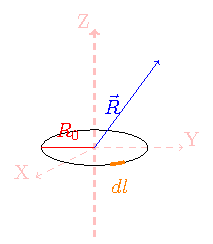
\includegraphics[width=0.5\linewidth]{electromagnetismo_2018_10_10_1}
\par\end{center}

El valor del potencial en el eje $Z$ es muy fácil de calcular, de
hecho, lo podemos hallar de forma analítica:

\[
\lambda=\frac{q}{2\pi R_{0}}
\]

\[
\phi\left(0,0,z\right)=\frac{1}{4\pi\varepsilon_{0}}\frac{q}{\sqrt{R^{2}+z^{2}}}
\]
Sin embargo, fuera de el eje es difícil, por lo que usamos el desarrollo
multipolar. Ya tenemos $q$; ahora, calculemos $\vec{p}$:

\[
p_{x}=\int_{C'}\lambda x'dl'=\lambda\int_{0}^{2\pi}R_{0}\cos\varphi'R_{0}d\varphi'=0
\]

\[
p_{y}=\int_{C'}\lambda y'dl'=0
\]

\[
p_{z}=\int_{C'}\lambda z'dl'=0
\]
Es decir: 

\[
\vec{p}=\vec{0}
\]
Podemos ver esto gráficamente mediante:
\begin{center}
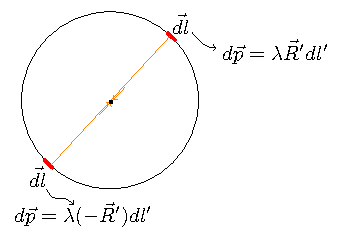
\includegraphics[width=0.5\linewidth]{electromagnetismo_2018_10_10_2}
\par\end{center}

Debido a la simetría respecto al eje $Z$ no hay momento dipolar.
Ahora, toca calcular los $Q'_{xy}$.

\[
Q'_{xy}=Q'_{yx}=\int_{C'}x'y'\lambda dl'=\lambda\int_{0}^{2\pi}R_{0}\cos\varphi'R_{0}\sin\varphi'R_{0}d\varphi'=
\]

\[
=\lambda R_{0}^{3}\int_{0}^{2\pi}\sin\varphi'\cos'd\varphi'=\frac{\lambda R_{0}^{3}}{2}\left[\sin^{2}\varphi\right]_{0}^{2\pi}=0
\]

\[
Q'_{zz}=0
\]

\[
Q'_{xx}=\int_{C'}x'\,^{2}\lambda dl'=\lambda\int R_{0}^{2}\cos^{2}\varphi'R_{0}d\varphi'=\lambda R_{0}^{3}\int_{0}^{2\pi}\cos^{2}\varphi'd\varphi'
\]
Sabiendo $\int\cos^{2}\varphi d\varphi=\frac{\varphi}{2}+\frac{\sin2\varphi}{4}$,
obtenemos:

\[
=\lambda R_{0}^{3}\left[\frac{\varphi}{2}+\frac{\sin2\varphi}{4}\right]_{0}^{2\pi}=\lambda R_{0}^{3}\left(\frac{2\pi}{2}+0-0-0\right)=\lambda\pi R_{0}^{3}
\]
Nótese que:

\[
Q'_{yy}=Q'_{xx}
\]
por simetría. Por último:

\[
Q'_{zx}=Q'_{xz}=0=Q'_{yz}=Q'_{zy}
\]
porque $z'=0$ en todo el anillo. Por consiguiente:

\[
\phi\left(\vec{R}\right)=\frac{1}{4\pi\varepsilon_{0}}\left(\frac{q}{R}+0+\frac{1}{2}\left[\frac{3x^{2}-R^{2}}{R^{5}}\lambda\pi R_{0}^{3}+\frac{3y^{2}-R^{2}}{R^{5}}\lambda\pi R_{0}^{3}\right]+\dots\right)=
\]

\[
=\frac{1}{4\pi\varepsilon_{0}}\left(\frac{q}{R}+\frac{\lambda\pi R_{0}^{3}}{2}\frac{3\left(x^{2}+y^{2}\right)-2R^{2}}{R^{5}}+\dots\right)
\]
Recordando ${\displaystyle \lambda=\frac{q}{2\pi R_{0}}}$, llegamos
a:

\[
\frac{\lambda\pi R_{0}^{3}}{2}=\frac{qR_{0}^{2}}{4}
\]
Sustituyendo:

\[
\phi\left(\vec{R}\right)=\frac{q}{4\pi\varepsilon_{0}R}\left(1+\frac{R_{0}^{2}}{4R^{4}}\left[3\left(x^{2}+y^{2}\right)-2R^{2}\right]+\dots\right)
\]
Teniendo en cuenta $R^{2}=x^{2}+y^{2}+z^{2}$:

\[
\phi\left(\vec{R}\right)=\frac{q}{4\pi\varepsilon_{0}R}\left(1+\frac{R_{0}^{2}}{R^{4}}\frac{x^{2}+y^{2}-2z^{2}}{4}+\dots\right)
\]
\end{example}
%
\begin{example}[$R=10R_{0}$ en el eje $z$]

En las mismas condiciones que en el ejemplo anterior, vamos a calcular
$\phi\left(0,0,10R_{0}\right)$. Para este caso, también tenemos una
solución exacta; de manera que podremos comparar.

\[
\phi_{\approx}\left(0,0,10R_{0}\right)\approx\frac{1}{4\pi\varepsilon_{0}}\frac{Q}{10R_{0}}\left(1+\frac{R_{0}^{2}}{\left(10R_{0}\right)^{4}}\frac{-2\left(10R_{0}\right)^{2}}{4}\right)=\frac{1}{4\pi\varepsilon_{0}}\frac{Q}{10R_{0}}\left(1-\frac{1}{200}\right)
\]
Podemos ver que:

\[
\frac{\phi_{\text{cuadrupolar}}}{\phi_{\text{monopolar}}}=\frac{1}{200}=0,5\%
\]
Por otra parte, el potencial exacto es:

\[
\phi_{=}\left(z=10R_{0}\right)=\frac{1}{4\pi\varepsilon_{0}}\frac{Q}{\sqrt{101}R_{0}}
\]

\[
\frac{\phi_{\text{monopolar}}}{\phi_{=}}=\frac{\sqrt{101}}{10}=1,00498\Rightarrow\text{Error relativo del }0,5\%
\]

\[
\frac{\phi_{\approx}}{\phi_{=}}=0,9999626\Rightarrow\text{Error relativo de }3,74\cdot10^{-5}
\]
\end{example}
%
\begin{example}[$z=0$, $R=10R_{0}$]

Nos encontramos en las mismas condiciones que en el ejemplo \vref{exa:Prob27}
y queremos calcular el potencial para las condiciones $z=0$, $R=10R_{0}$.
Entonces:

\[
R^{2}=x^{2}+y^{2}=\left(10R_{0}\right)^{2}
\]
El término aproximado es:

\[
\phi_{\approx}\left(x,y,0\right)\approx\frac{1}{4\pi\varepsilon_{0}}\frac{Q}{10R_{0}}\left(1+\frac{R_{0}^{2}}{\left(10R_{0}\right)^{4}}\frac{\left(10R_{0}\right)^{2}}{4}\right)=\frac{1}{4\pi\varepsilon_{0}}\frac{Q}{10R_{0}}\left(1+\frac{1}{400}\right)
\]
Podemos calcular el cociente:

\[
\frac{\phi_{\text{cuadrupolar}}}{\phi_{\text{monopolar }}}=\frac{1}{400}=0,25\%
\]
\end{example}
%
\begin{example}[Problema 26]

Tenemos la siguiente distribución de cargas puntuales (un octupolo).
\begin{center}
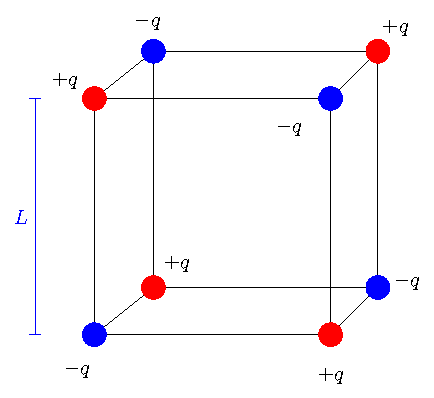
\includegraphics[width=0.5\linewidth]{electromagnetismo_2018_10_10_3}
\par\end{center}

Claramente, la carga total es nula:

\[
q_{T}=0
\]
Ahora, obtengamos la densidad de carga expresada mediante la delta
de Dirac.

\[
\rho\left(R'\right)=q\delta\left(x',y',z'\right)-q\delta\left(x'-L,y',z'\right)+q\delta\left(x'-L,y'-L,z'\right)-q\left(x',y'-L,z'\right)+
\]

\[
q\delta\left(x',y'-L,z'-L\right)-q\delta\left(x',y',z'-L\right)+q\delta\left(x'-L,y',z'-L\right)-q\delta\left(x'-L,y'-L,z'-L\right)
\]
Lo siguiente es calcular el momento dipolar.

\[
\vec{p}=\iiint_{V'}\rho\left(\vec{R}'\right)\cdot\vec{R}'dV'=q\left(0,0,0\right)-q\left(L,0,0\right)+q\left(L,L,0\right)-q\left(0,L,0\right)+q\left(0,L,L\right)-q\left(0,0,L\right)+
\]

\[
q\left(L,0,L\right)-q\left(L,L,L\right)=q\left(0,0,0\right)=\vec{0}
\]
Y ahora los momentos cuadrupolares:

\[
Q_{xx}=\iiint_{V'}\rho\left(\vec{R}'\right)x'^{2}dV'=q\left(-L^{2}+L^{2}-L^{2}+L^{2}\right)=0
\]

\[
Q_{yy}=0=Q_{zz}
\]

\[
Q_{xy}=Q_{yx}=0=Q_{xz}=Q_{zx}
\]
Nótese que como lo que tenemos un octupolo, es lógico que los términos
de orden cero, uno y dos del desarrollo de Taylor (carga puntual,
momento dipolar y momento cuadrupolar) salgan cero. Es decir, si nos
quedamos a orden dos, el potencial creado por un octupolo es:

\[
\phi_{\approx}\approx0
\]
\end{example}

\section{Simplificación de la expresión}
\begin{prop}
\label{prop:El-desarrollo-multipolar}El desarrollo multipolar del
potencial generado por una distribución de carga cualquiera puede
ser expresado como:

\[
\phi\left(\vec{R}\right)=\frac{1}{4\pi\varepsilon_{0}}\left[\frac{q}{R}+\frac{\vec{p}\cdot\vec{R}}{R^{3}}+\frac{1}{2}\sum_{i=1}^{3}\sum_{j=1}^{3}\frac{x_{i}x_{j}}{R^{5}}Q_{ij}+\dots\right]
\]
donde $q$ es la carga, $\vec{p}=\iiint_{V'}\rho\left(\vec{R}'\right)\vec{R}'dV'$
y $Q_{ij}=\iiint_{V'}\rho\left(\vec{R}'\right)\left(3x_{i}'x_{j}'-R'^{2}\delta_{ij}\right)dV'$.
\end{prop}
\begin{proof}
Recordemos la proposición \vref{prop:DesarrolloMultipolarQPrima}:

\[
\phi\left(\vec{R}\right)=\frac{1}{4\pi\varepsilon_{0}}\left[\frac{q}{R}+\frac{\vec{p}\cdot\vec{R}}{R^{3}}+\frac{1}{2}\sum_{i=1}^{3}\sum_{j=1}^{3}\frac{3x_{i}x_{j}-\delta_{ij}R^{2}}{R^{5}}Q'_{ij}+\dots\right]
\]
Del doble sumatorio correspondiente al término de segundo orden, calculamos:

\[
\sum_{i=1}^{3}\frac{3x_{i}x_{i}-\delta_{ii}R^{2}}{R^{5}}Q'_{ii}=\sum_{i=1}^{3}\frac{3x_{i}^{2}-R^{2}}{R^{5}}Q'_{ii}=
\]

\[
=\frac{3x_{1}^{2}-R^{2}}{R^{5}}\iiint_{V'}x'\,_{1}^{2}\rho\left(\vec{R}'\right)dV'+\frac{3x_{2}^{2}-R^{2}}{R^{5}}\iiint_{V'}x'\,_{2}^{2}\rho\left(\vec{R}'\right)dV'+\frac{3x_{3}^{2}-R^{2}}{R^{5}}\iiint_{V'}x'\,_{3}^{2}\rho\left(\vec{R}'\right)dV'=
\]

\[
=\iiint_{V'}\frac{\left(3x_{1}^{2}-R^{2}\right)x'\,_{1}^{2}+\left(3x_{2}^{2}-R^{2}\right)x'\,_{2}^{2}+\left(3x_{3}^{2}-R^{2}\right)x'\,_{3}^{2}}{R^{5}}\rho\left(\vec{R}'\right)dV'=
\]

\[
=\iiint_{V'}\frac{3x_{1}^{2}x'\,_{1}^{2}+3x_{2}^{2}x'\,_{2}^{2}+3x_{3}^{2}x'\,_{3}^{2}-R^{2}\left(x'\,_{1}^{2}+x'\,_{2}^{2}+x'\,_{3}^{2}\right)}{R^{5}}\rho\left(\vec{R}'\right)dV'=
\]

\[
=\iiint_{V'}\frac{3x_{1}^{2}x'\,_{1}^{2}+3x_{2}^{2}x'\,_{2}^{2}+3x_{3}^{2}x'\,_{3}^{2}-\overbrace{R^{2}}^{=x_{1}^{2}+x_{2}^{2}+x_{3}^{2}}\cdot R'\,^{2}}{R^{5}}\rho\left(\vec{R}'\right)dV'=
\]

\[
=\iiint_{V'}\frac{\left(3x'\,_{1}^{2}-R'\,^{2}\right)x_{1}^{2}+\left(3x'\,_{2}^{2}-R'\,^{2}\right)x_{2}^{2}+\left(3x'\,_{3}^{2}-R'\,^{2}\right)x_{3}^{2}}{R^{5}}\rho\left(\vec{R}'\right)dV'=
\]

\[
=\frac{x_{1}^{2}}{R^{5}}\iiint_{V'}\left(x'\,_{1}^{2}-R\,'^{2}\right)\rho\left(\vec{R}'\right)dV'+\frac{x_{2}^{2}}{R^{5}}\iiint_{V'}\left(3x'\,_{2}^{2}-R'\,^{2}\right)\rho\left(\vec{R}'\right)dV+\frac{x_{3}^{2}}{R^{5}}\iiint_{V'}\left(3x'\,_{3}^{2}-R'\,^{2}\right)\rho\left(\vec{R}'\right)dV'
\]
Ahora, si definimos:

\[
Q_{ij}:=\iiint_{V'}\rho\left(\vec{R}'\right)\left(3x_{i}'x_{j}'-R'^{2}\delta_{ij}\right)dV'
\]
La expresión anterior quedaría:

\[
\sum_{i=1}^{3}\frac{3x_{i}x_{i}-\delta_{ii}R^{2}}{R^{5}}Q'_{ii}=\frac{x_{1}^{2}}{R^{5}}Q_{11}+\frac{x_{2}^{2}}{R^{5}}Q_{22}+\frac{x_{3}^{2}}{R^{5}}Q_{33}=\sum_{i=1}^{3}\frac{x_{i}^{2}}{R^{5}}Q_{ii}
\]
Por otra parte:

\[
\left[\frac{3x_{i}x_{j}-\delta_{ij}R^{2}}{R^{5}}Q'_{ij}\right]_{i\neq j}=\frac{3x_{i}x_{j}}{R^{5}}Q'_{ij}=\frac{3x_{i}x_{j}}{R^{5}}\iiint_{V'}x'_{i}x'_{j}\rho\left(\vec{R}'\right)dV'=
\]

\[
=\frac{x_{i}x_{j}}{R^{5}}\iiint_{V'}3x'_{i}x'_{j}\rho\left(\vec{R}'\right)dV'=\frac{x_{i}x_{j}}{R^{5}}\left[Q_{ij}\right]_{i\neq j}
\]
Es decir, podemos reescribir la suma:

\[
\sum_{i=1}^{3}\sum_{j=1}^{3}\frac{3x_{i}x_{j}-\delta_{ij}R^{2}}{R^{5}}Q'_{ij}=\sum_{i=1}^{3}\frac{3x_{i}^{2}-R^{2}}{R^{5}}Q'_{ii}+\sum_{\begin{matrix}i,j=1\\
i\neq j
\end{matrix}}^{3}\frac{3x_{i}x_{j}}{R^{5}}Q'_{ij}=
\]

\[
=\sum_{i=1}^{3}\frac{x_{i}^{2}}{R^{5}}Q_{ii}+\sum_{\begin{matrix}i,j=1\\
i\neq j
\end{matrix}}^{3}\frac{x_{i}x_{j}}{R^{5}}Q_{ij}=\sum_{i,j=1}^{3}\frac{x_{i}x_{j}}{R^{5}}Q_{ij}
\]
En consecuencia, obtenemos una expresión equivalente para el polinomio
de Taylor:

\[
\phi\left(\vec{R}\right)=\frac{1}{4\pi\varepsilon_{0}}\left[\frac{q}{R}+\frac{\vec{p}\cdot\vec{R}}{R^{3}}+\frac{1}{2}\sum_{i=1}^{3}\sum_{j=1}^{3}\frac{x_{i}x_{j}}{R^{5}}Q_{ij}+\dots\right]
\]
\end{proof}
\begin{rem}
\label{rem:Qxx+Qyy+Qzz}Esta nueva expresión alternativa tiene la
ventaja de que:

\[
Q_{xx}+Q_{yy}+Q_{zz}=\iiint_{V'}\rho\left(\vec{R}'\right)\left[3x'\,_{1}^{2}-R'^{2}+3x'\,_{2}^{2}-R'^{2}+3x'\,_{3}^{3}-R'\,^{2}\right]dV'=
\]

\[
=\iiint_{V'}\rho\left(\vec{R}'\right)\left[3\left(\underbrace{x'\,_{1}^{2}+x'\,_{2}^{2}+x\,'\,_{3}^{2}}_{=R'\,^{2}}\right)-3R'\,^{2}\right]=0
\]

Lo cual significa que hace falta calcular menos términos en la práctica.
\end{rem}

\section{Propiedades útiles para la obtención del desarrollo multipolar}

Recordemos que el momento dipolar se definía como:

\[
\vec{p}:=\iiint_{V'}\rho\left(\vec{R}'\right)\vec{R}'dV'
\]

Que se traduce en tres integrales (pues estamos en $\mathbb{R}^{3}$):

\[
p_{x}=\iiint_{V'}\rho\left(\vec{R}'\right)x'dV'
\]

\[
p_{y}=\iiint_{V'}\rho\left(\vec{R}'\right)y'dV'
\]

\[
p_{z}=\iiint_{V'}\rho\left(\vec{R}'\right)z'dV'
\]

\begin{prop}[Propiedades del momento dipolar]
~
\begin{enumerate}
\item Si el origen es el centro de simetría, entonces $\vec{p}=\vec{0}$.
\item Si por el origen pasa un plano de simetría, entonces $\vec{p}$ estará
contenido en dicho plano.
\item Si por el origen pasa un eje de simetría, entonces $\vec{p}$ estará
contenido en dicho eje.
\end{enumerate}
\end{prop}
\begin{proof}
~
\begin{enumerate}
\item Si el origen de cargas es un centro de simetría, entonces $\rho\left(\vec{R}\right)=\rho\left(-\vec{R}\right)\;\forall\vec{R}\in V$.
Recordemos que, por la proposición \vref{prop:El-desarrollo-multipolar}
es:
\[
\vec{p}=\iiint_{V}\rho\left(\vec{R}\right)\vec{R}dV
\]
Ahora, podemos dividir la integral al volumen en dos integrales, lo
que hay del plano $z=0$ hacia arriba (a lo que llamaremos $V+$)
y lo que hay del plano $z=0$ hacia abajo (lo que llamaremos $V-$).
Así:
\[
\vec{p}=\iiint_{V}\rho\left(\vec{R}\right)\vec{R}dV=\iiint_{V+}\rho\left(\vec{R}\right)\vec{R}dV+\iiint_{V-}\rho\left(\vec{R}\right)\vec{R}dV=\iiint_{V+}\left[\rho\left(\vec{R}\right)\vec{R}+\rho\left(-\vec{R}\right)\left(-\vec{R}\right)\right]dV
\]
Como $\rho\left(-\vec{R}\right)=\rho\left(\vec{R}\right)$, podemos
expresar la integral anterior como:
\[
\vec{p}=\iiint_{V+}\rho\left(\vec{R}\right)\left(\vec{R}-\vec{R}\right)dV=\vec{0}
\]
\item Podemos suponer, sin pérdida de generalidad, que el plano de simetría
es el $XY$. Por tanto, sabemos que: $\rho\left(x,y,z\right)=\rho\left(x,y,-z\right)\;\forall\left(x,y,z\right)\in V$.
Si la componente $p_{z}$ es nula, entonces $\vec{p}$ necesariamente
estará en el plano $XY$. Veámoslo, por la proposición \vref{prop:El-desarrollo-multipolar},
tenemos:
\[
p_{z}=\iiint_{V}\rho\left(x,y,z\right)zdV
\]
De nuevo, podemos dividir la integral al volumen en dos integrales,
lo que hay del plano $z=0$ hacia arriba (a lo que llamaremos $V+$)
y lo que hay del plano $z=0$ hacia abajo (lo que llamaremos $V-$).
Así:
\[
p_{z}=\iiint_{V+}\rho\left(x,y,z\right)zdV+\iiint_{V-}\rho\left(x,y,z\right)dV=\iiint_{V+}\left[\rho\left(x,y,z\right)z+\rho\left(x,y,-z\right)\left(-z\right)\right]dV
\]
Como $\rho\left(x,y,z\right)=\rho\left(x,y,-z\right)\;\forall\left(x,y,z\right)\in V$,
tenemos:
\[
p_{z}=\iiint_{V+}\rho\left(x,y,z\right)\left(z-z\right)dV=0
\]
\item Podemos suponer, sin pérdida de generalidad, que el eje de simetría
es el eje $z$. Si $z$ es eje de simetría, entonces los planos $XZ$
e $YZ$ también serán de simetría. En consecuencia, por $\left(2\right)$
será $p_{x}=0=p_{y}$ y, por ende, $\vec{p}$ únicamente tiene componente
$z$.
\end{enumerate}
\end{proof}
Podemos ver el primer punto gráficamente mediante:
\begin{center}
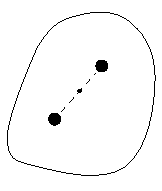
\includegraphics[width=0.4\linewidth]{electromagnetismo_2018_10_16_1}
\par\end{center}

porque, si el origen es el centro de simetría, entonces, por cada
$d\vec{p}$ que ejerza un $dV$ de la distribución debe existir otro
$dV$ que ejerza menos $-d\vec{p}$. Si la distribución no es uniforme,
de manera que el origen no es centro de simetría, podemos ver claramente
que $\vec{p}\neq\vec{0}$ con el siguiente ejemplo:
\begin{center}
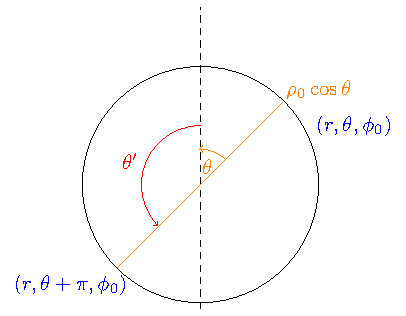
\includegraphics[width=0.6\linewidth]{electromagnetismo_2018_10_16_3}
\par\end{center}

donde $\rho\left(r,\theta,\phi\right)=\rho_{0}\cos\theta$.
\begin{prop}[Propiedades del momento cuadrupolar]
~
\begin{enumerate}
\item Si hay un eje de revolución (llamémoslo, por conveniencia, eje $z$)
de la distribución, entonces:
\[
Q_{xy}=Q_{yz}=Q_{xz}=0
\]
\[
Q_{xx}=Q_{yy}=-\frac{1}{2}Q_{zz}
\]
Como se cumple $Q_{xx}+Q_{yy}+Q_{zz}=0$, en forma matricial tendríamos:
\[
\left(Q_{ij}\right)=\left(\begin{matrix}-\frac{1}{2} & 0 & 0\\
0 & -\frac{1}{2} & 0\\
0 & 0 & 1
\end{matrix}\right)
\]
Y en consecuencia, en coordenadas esféricas, se tiene:
\[
\phi_{\text{cuadrupolar}}=\frac{Q_{zz}}{4\pi\varepsilon_{0}}\frac{3\cos^{2}\theta-1}{4R^{3}}
\]
\item Si el plano $XY$ es de simetría, es decir, $\rho\left(x_{0},y_{0},z\right)=\rho\left(x_{0},y_{0},-z\right)$,
entonces:
\[
Q_{xz}=0=Q_{yz}
\]
\item Si la distribución es antisimétrica, es decir, $\rho\left(-x',-y',-z'\right)=-\rho\left(x',y',z'\right)$,
entonces:
\[
\left(Q_{ij}\right)=\left(0\right)
\]
Y lo mismo ocurre para cualquier momento de orden par.
\end{enumerate}
\end{prop}
\begin{proof}
~
\begin{enumerate}
\item[$2$] Si el plano $XY$ es de simetría, entonces $\rho\left(x,y,z\right)=\rho\left(x,y,-z\right)\;\forall\left(x,y,z\right)\in V$.
Por la proposición \vref{prop:El-desarrollo-multipolar}, tenemos:
\[
Q_{ij}=\iiint_{V}\rho\left(x_{1},x_{2},x_{3}\right)\left(3x_{i}x_{j}-R^{2}\delta_{ij}\right)
\]
En particular, tenemos:
\[
Q_{xz}=\iiint_{V}\rho\left(x,y,z\right)3xzdV
\]
Podemos dividir el volumen anterior en el volumen que hay por encima
del plano $z=0$ (al que llamaremos $V+$) y el que hay por debajo
(al que llamaremos $V-$). En consecuencia, tenemos:
\[
Q_{xz}=\iiint_{V+}\rho\left(x,y,z\right)3xzdV+\iiint_{V-}\rho\left(x,y,z\right)3xzdV=\iiint_{V+}\left[\rho\left(x,y,z\right)3xz+\rho\left(x,y,-z\right)3x\left(-z\right)\right]dV
\]
Como $\rho\left(x,y,z\right)=\rho\left(x,y,-z\right)$, tenemos:
\[
Q_{xz}=\iiint_{V+}3\rho\left(x,y,z\right)x\left(z-z\right)dV=0
\]
Análogamente sucede con el $Q_{yz}$. Así:
\[
Q_{xz}=0=Q_{yz}
\]
\item[$1$] Si $Z$ es un eje de revolución de mi sistema, entonces, los planos
$XZ$ e $YZ$ son planos de simetría de mi sistema. Por $\left(2\right)$,
serán $Q_{xy}=Q_{yz}=Q_{xz}=0$.\\
Por otra parte, como $Z$ es un eje de revolución del sistema, será
$\rho\left(r\cos\theta_{1},r\sin\theta_{1},z\right)=\rho\left(r\cos\theta_{2},r\cos\theta_{2},z\right)\;\forall\theta_{1},\theta_{2},r,z\in\mathbb{R}$.
En otras palabras, $\rho$ únicamente depende de la distancia al eje
$z$; a dicha distancia la llamamos $r$. En consecuencia, pasando
la integral a cilíndricas ($x=r\cos\theta;y=r\sin\theta$), obtenemos:
\[
Q_{xx}=\iiint_{V}\rho\left(x,y,z\right)\left(3x^{2}-\sqrt{x^{2}+y^{2}+z^{2}}\right)dV=
\]
\[
=\iiint_{V}\rho\left(r,z\right)\left(3r^{2}\cos^{2}\theta-\sqrt{r^{2}\cos^{2}\theta+r^{2}\sin^{2}\theta+z^{2}}\right)dV=
\]
\[
=\iiint_{V}\rho\left(r,z\right)\left(3r^{2}\cos^{2}\theta-\sqrt{r^{2}+z^{2}}\right)dV=
\]
\[
=\int_{r=0}^{\infty}\int_{z=-\infty}^{\infty}\int_{\theta=0}^{2\pi}\rho\left(r,z\right)\left(3r^{2}\cos^{2}\theta-\sqrt{r^{2}+z^{2}}\right)rdrd\theta dz
\]
Ahora, como la densidad de carga $\rho$ no depende de $\theta$,
sale fuerza de la integral. En consecuencia, llegamos a:
\begin{equation}
Q_{xx}=\int_{r=0}^{\infty}\int_{z=-\infty}^{\infty}\rho\left(r,z\right)\left[3r^{2}\int_{\theta=0}^{2\pi}\cos^{2}\theta d\theta-2\pi\sqrt{r^{2}+z^{2}}\right]rdrdz\label{eq:Qxx}
\end{equation}
Resolvamos la integral del coseno aparte:
\begin{equation}
\int_{0}^{2\pi}\cos^{2}\theta d\theta\label{eq:Integral cos^2}
\end{equation}
Por el coseno del ángulo doble, tenemos:
\[
\cos^{2}\theta-\sin^{2}\theta=\cos\frac{\theta}{2}\Leftrightarrow\cos^{2}\theta-\left(1-\cos^{2}\theta\right)=\cos\frac{\theta}{2}\Leftrightarrow2\cos^{2}\theta-1=\cos\frac{\theta}{2}\Leftrightarrow
\]
\[
\cos^{2}\theta=\frac{1}{2}+\cos\frac{\theta}{2}
\]
Sustituyendo en la ecuación \vref{eq:Integral cos^2}, obtenemos:
\[
\int_{0}^{2\pi}\cos^{2}\theta d\theta=\int_{0}^{2\pi}\left(\frac{1}{2}+\cos\frac{\theta}{2}\right)d\theta=\left[\frac{\theta}{2}+\frac{1}{2}\sin\frac{\theta}{2}\right]_{0}^{2\pi}=\pi+\frac{1}{2}\sin\pi-0-\frac{1}{2}\sin0=\pi
\]
Por otra parte, la siguiente integral:
\[
\int_{0}^{2\pi}\sin^{2}\theta d\theta=\int_{0}^{2\pi}\left(1-\cos^{2}\theta\right)d\theta=\left[\theta-\frac{\theta}{2}-\frac{1}{2}\sin\frac{\theta}{2}\right]_{0}^{2\pi}=\left[\frac{\theta}{2}-\frac{1}{2}\sin\frac{\theta}{2}\right]_{0}^{2\pi}=
\]
\[
\pi-\frac{1}{2}\sin\pi-0+\frac{1}{2}\sin0=\pi
\]
En consecuencia, podemos sustituir en la ecuación \vref{eq:Qxx} la
integral del coseno por la integral del seno, pues dan el mismo resultado:
\[
Q_{xx}=\int_{r=0}^{\infty}\int_{z=-\infty}^{\infty}\rho\left(r,z\right)\left[3r^{2}\int_{\theta=0}^{2\pi}\sin^{2}\theta d\theta-2\pi\sqrt{r^{2}+z^{2}}\right]rdrdz=
\]
\[
=\int_{r=0}^{\infty}\int_{z=-\infty}^{\infty}\int_{\theta=0}^{2\pi}\rho\left(r,z\right)\left[3r^{2}\sin^{2}\theta-\sqrt{r^{2}+z^{2}}\right]rdrdzd\theta=\iiint_{V}\rho\left(r,z\right)\left[3r^{2}\sin^{2}\theta-\sqrt{r^{2}+z^{2}}\right]dV
\]
Deshaciendo el cambio a cartesianas, recordando $y=r\sin\theta$,
obtenemos:
\[
Q_{xx}=\iiint_{V}\rho\left(x,y,z\right)\left[3y^{2}-\sqrt{x^{2}+y^{2}+z^{2}}\right]dV=Q_{yy}
\]
Por último, por la observación \vref{rem:Qxx+Qyy+Qzz}, debe ser:
\[
Q_{xx}+Q_{yy}+Q_{zz}=0\Leftrightarrow2Q_{xx}+Q_{zz}=0\Leftrightarrow Q_{zz}=-\frac{1}{2}Q_{xx}=-\frac{1}{2}Q_{yy}
\]
\item[$3$] Si la distribución de carga es antisimétrica, entonces es $\rho\left(x,y,z\right)=-\rho\left(-x,-y,-z\right)\;\forall\left(x,y,z\right)$.
Por la proposición \vref{prop:El-desarrollo-multipolar} tenemos que:
\[
Q_{ij}=\iiint_{V}\rho\left(\vec{R}\right)\left(3x_{i}x_{j}-R{}^{2}\delta_{ij}\right)dV
\]
Podemos dividir el volumen $V$ en la parte que se encuentra sobre
el plano $z=0$ ($V+$) y la parte que se encuentra por debajo del
plano $z=0$ ($V-$). Así:
\[
Q_{ij}=\iiint_{V+}\rho\left(x_{1},x_{2},x_{3}\right)\left(3x_{i}x_{j}-R^{2}\delta_{ij}\right)dV+\iiint_{V-}\rho\left(x_{1},x_{2},x_{3}\right)\left(3x_{i}x_{j}-R^{2}\delta_{ij}\right)dV=
\]
\[
=\iiint_{V+}\left[\rho\left(x_{1},x_{2},x_{3}\right)\left(3x_{i}x_{j}-\left(x^{2}+y^{2}+z^{2}\right)\delta_{ij}\right)+\right.
\]
\[
\left.+\rho\left(-x_{1},-x_{2},-x_{3}\right)\left(3\left(-x_{i}\right)\left(-x_{j}\right)-\left(\left(-x\right)^{2}+\left(-y\right)^{2}+\left(-z\right)^{2}\right)\delta_{ij}\right)\right]dV
\]
Como $\rho\left(x_{1},x_{2},x_{3}\right)=-\rho\left(x_{1},x_{2},x_{3}\right)$,
tenemos que:
\[
Q_{ij}=\iiint_{V+}\rho\left(x_{1},x_{2},x_{3}\right)\left(3x_{i}x_{j}-R^{2}\delta_{ij}-\left(3x_{i}x_{j}-R^{2}\delta_{ij}\right)\right)dV=0
\]
Y como lo anterior es válido $\forall i,j=1,2,3$, concluimos que
$\left(Q_{ij}\right)=\left(0\right)$.
\end{enumerate}
\end{proof}
Podemos ver el primer punto gráficamente:
\begin{center}
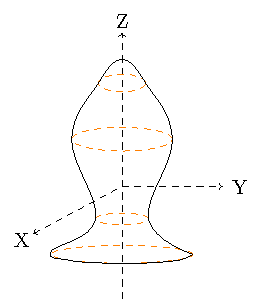
\includegraphics[width=0.6\linewidth]{electromagnetismo_2018_10_16_2}
\par\end{center}
\begin{prop}[Efecto de la elección del origen]
~
\begin{enumerate}
\item Si $Q=0$, entonces $\vec{p}$ es independiente del origen.
\item Si $Q\neq0$ y se toma el origen en el centro de cargas del sistema
$\vec{a}={\displaystyle \frac{{\displaystyle \sum_{i=1}^{n}q_{i}\vec{r}_{i}}}{Q}}$,
entonces $\vec{p}=\vec{0}$.
\item Si $Q=0$ y $\vec{p}=\vec{0}$, entonces los $Q_{ij}$ son independientes
del origen.
\end{enumerate}
\end{prop}
\begin{proof}
~
\begin{enumerate}
\item Sea $S=\left(O;\vec{R}\right)$ un sistema de referencia afín y sea
$S'=\left(O';\vec{R}'\right)$ otro sistema de referencia afín. Entonces,
, por la proposición \vref{prop:El-desarrollo-multipolar}, el momento
dipolar $\vec{p}$ calculado por $S$ es:
\[
\vec{p}=\iiint_{V}\rho\left(\vec{R}\right)\vec{R}dV=\iiint_{V}\rho\left(\overrightarrow{OO'}+\vec{R}'\right)\left(\overrightarrow{OO'}+\vec{R}'\right)dV=
\]
\[
=\iiint_{V}\rho\left(\overrightarrow{OO'}+\vec{R}'\right)\overrightarrow{OO'}dV+\iiint_{V}\rho\left(\overrightarrow{OO'}+\vec{R}'\right)dV=
\]
\[
=\overrightarrow{OO'}\underbrace{\iiint_{V}\rho\left(\overrightarrow{OO'}+\vec{R}'\right)dV}_{=Q}+\iiint_{V}\rho\left(\overrightarrow{OO'}+\vec{R}'\right)dV=\overrightarrow{OO'}Q+\vec{p}'=\vec{p}'
\]
donde el primer sumando se anula al ser $Q=0$ por hipótesis. En consecuencia,
el momento dipolar es el mismo desde cualquier sistema de referencia;
dicho de otra forma, no depende del origen.
\item Si el origen del sistema de coordenadas es el centro de carga, entonces:
\begin{equation}
\frac{{\displaystyle \sum_{i=1}^{n}q_{i}\vec{R}_{i}}}{Q}=\vec{0}\Leftrightarrow\sum_{i=1}^{n}q_{i}\vec{R}_{i}=\vec{0}\label{eq:qiRi=00003D0}
\end{equation}
En este caso, como tenemos un número finito de cargas, la integral
que usamos para calcular el momento dipolar $\vec{p}$ se reduce a
un sumatorio.
\[
\vec{p}=\iiint_{V}\rho\left(\vec{R}\right)\vec{R}dV=\sum_{i=1}^{n}q_{i}\vec{R}_{i}=\vec{0}
\]
donde lo anterior se cumple por la ecuación \vref{eq:qiRi=00003D0}.
\item Sea $S=\left(O;\vec{R}\right)$ un sistema de referencia afín y sea
$S'=\left(O';\vec{R}'\right)$ otro sistema de referencia afín. Entonces,
por la proposición \vref{prop:El-desarrollo-multipolar}, el momento
cuadrupolar $Q_{ij}$ visto desde el sistema $S$:
\[
Q_{ij}=\iiint_{V}\rho\left(\vec{R}\right)\left(3x_{i}x_{j}-R^{2}\delta_{ij}\right)dV=
\]
\[
\iiint_{V}\rho\left(\overrightarrow{OO'}+\vec{R}'\right)\left[3\left(\overrightarrow{OO'}_{i}+x_{i}'\right)\left(\overrightarrow{OO'}_{j}+x_{j}'\right)-\left(\overrightarrow{OO'}^{2}+R'\,^{2}\right)\delta_{ij}\right]dV=
\]
\[
=\iiint_{V}3\rho\left(\overrightarrow{OO'}+\vec{R}'\right)\overrightarrow{OO'}_{i}\overrightarrow{OO'}_{j}dV+\iiint_{V}3\rho\left(\overrightarrow{OO'}+\vec{R}'\right)x_{i}'\overrightarrow{OO'}_{j}dV+
\]
\[
+\iiint_{V}3\rho\left(\overrightarrow{OO'}+\vec{R}'\right)\overrightarrow{OO'}_{i}x_{i}'dV+\iiint_{V}3\rho\left(\overrightarrow{OO'}+\vec{R}'\right)x_{i}'x_{j}'dV+
\]
\[
-\iiint_{V}\delta_{ij}\rho\left(\overrightarrow{OO'}+\vec{R}'\right)\overrightarrow{OO'}^{2}dV-\iiint_{V}\delta_{ij}\rho\left(\overrightarrow{OO'}+\vec{R}'\right)R'\,^{2}dV=
\]
\[
=3\overrightarrow{OO'}_{i}\overrightarrow{OO'}_{j}\underbrace{\iiint_{V}\rho\left(\overrightarrow{OO'}+\vec{R}'\right)dV}_{=Q}+3\overrightarrow{OO'}_{j}\underbrace{\iiint_{V}\rho\left(\overrightarrow{OO'}+\vec{R}'\right)x_{i}'dV}_{=p_{i'}}+
\]
\[
+3\overrightarrow{OO'}_{i}\underbrace{\iiint_{V}\rho\left(\overrightarrow{OO'}+\vec{R}'\right)x_{j}'dV}_{=p_{j'}}+\iiint_{V}3\rho\left(\overrightarrow{OO'}+\vec{R}'\right)x_{i}'x_{j}'dV+
\]
\[
-\delta_{ij}\overrightarrow{OO'}^{2}\underbrace{\iiint_{V}\rho\left(\overrightarrow{OO'}+\vec{R}'\right)dV}_{=Q}-\iiint_{V}\delta_{ij}\rho\left(\overrightarrow{OO'}+\vec{R}'\right)R'\,^{2}dV=
\]
\[
=3\overrightarrow{OO'}_{i}\overrightarrow{OO'}_{j}Q+3\overrightarrow{OO'}_{j}p_{i'}+3\overrightarrow{OO'}_{i}p_{j'}-\delta_{ij}\overrightarrow{OO'}^{2}Q+Q_{ij}'
\]
Como, por hipótesis, es $\vec{p}=\vec{0}$ y $Q=0$, obtenemos que
$Q_{ij}=Q_{ij}'$. En otras palabras, el momento cuadrupolar no depende
del sistema de referencia.
\end{enumerate}
\end{proof}

\section{Capa dipolar}
\begin{defn}
Llamamos \textbf{capa dipolar} a una distribución de carga como:
\begin{center}
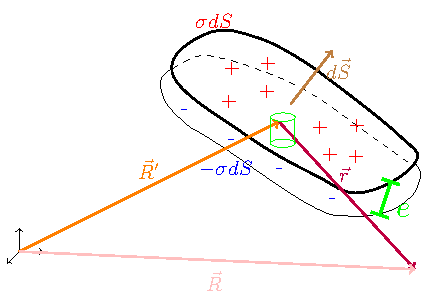
\includegraphics[width=0.6\linewidth]{electromagnetismo_2018_10_15_1}
\par\end{center}

Es decir, una capa dipolar son dos placas planas paralelas conductoras
cargadas separadas una distancia $e$ tales que la densidad de carga
evaluada en la intersección de cualquier recta $t$ perpendicular
a las superficies con la primera superficie tiene justo el valor opuesto
de la densidad de carga evaluada en la intersección de esa misma recta
$t$ con la segunda superficie. En otras palabras, se trata de dos
superficies planas paralelas $S_{1}$ y $S_{2}$ separadas una distancia
$e$ tales que:

\[
\sigma_{1}\left(\vec{R}\right)=-\sigma_{2}\left(\vec{R}+e\hat{S}\right)\;\forall\vec{R}\in S_{1}
\]
\end{defn}
\begin{prop}
\label{prop:PhiCapaDipolar}El potencial generado por una capa dipolar
de densidad de carga $\sigma$ y espesor $e$ viene dado por la expresión:

\[
\phi\left(\vec{R}\right)=\frac{-\tau}{4\pi\varepsilon_{0}}\iint d\Omega=-\frac{\tau}{4\pi\varepsilon_{0}}\Omega
\]
donde $\Omega$ es el ángulo sólido con el que se ve la capa dipolar
desde el punto $\vec{R}$ y $\tau=\sigma e$.
\end{prop}
\begin{proof}
Usando la definición \vref{def:p Dipolar}, obtenemos el diferencial
de momento dipolar es:
\begin{center}
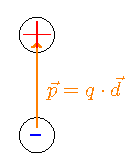
\includegraphics[width=0.3\linewidth]{electromagnetismo_2018_10_15_2}
\par\end{center}

\[
d\vec{p}=dq\cdot\vec{e}=\sigma dS\cdot\vec{e}
\]
Recordando la proposición \vref{prop:PhiDipolo}, obtenemos:

\[
d\phi\left(\vec{R}\right)=\frac{1}{4\pi\varepsilon_{0}}\frac{d\vec{p}\cdot\vec{r}}{r^{3}}=\frac{1}{4\pi\varepsilon_{0}}\frac{\overbrace{\sigma e}^{=:\tau}\vec{r}\cdot d\vec{S}}{r^{3}}=\frac{\tau}{4\pi\varepsilon_{0}}\frac{\vec{r}\cdot d\vec{S}}{r^{3}}
\]
donde ${\displaystyle \tau=\frac{dp}{dS}=\sigma e}$. Nótese que el
$dS$ va de la carga negativa a la positiva:
\begin{center}
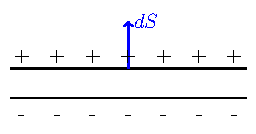
\includegraphics[width=0.7\linewidth]{electromagnetismo_2018_10_15_3}
\par\end{center}

Por otra parte, por la definición \vref{def:AngSol}, ${\displaystyle \frac{-\vec{r}\cdot d\vec{S}}{r^{3}}}$
es justo el ángulo sólido visto desde el punto $\vec{R}$. Por tanto:

\[
d\phi\left(\vec{R}\right)=-\frac{\tau}{4\pi\varepsilon_{0}}\frac{-\vec{r}\cdot d\vec{S}}{r^{3}}=\frac{-\tau}{4\pi\varepsilon_{0}}d\Omega
\]
Integrando, obtenemos:

\[
\phi\left(\vec{R}\right)=\frac{-\tau}{4\pi\varepsilon_{0}}\iint d\Omega=-\frac{\tau}{4\pi\varepsilon_{0}}\Omega
\]
\end{proof}
\begin{rem}
Si hubiéramos cogido el punto $\vec{R}$ en otro lugar, la representación
gráfica habría sido:
\begin{center}
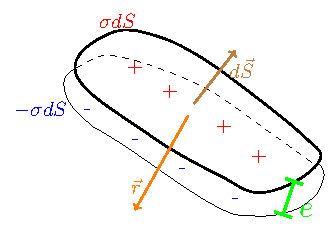
\includegraphics[width=0.6\linewidth]{electromagnetismo_2018_10_16_5}
\par\end{center}

\end{rem}
\textcolor{green}{}
%
\begin{rem}
Observemos una representación del potencial frente a la distancia
a la capa dipolar en el caso particular de $\sigma=\text{cte}$:
\begin{center}
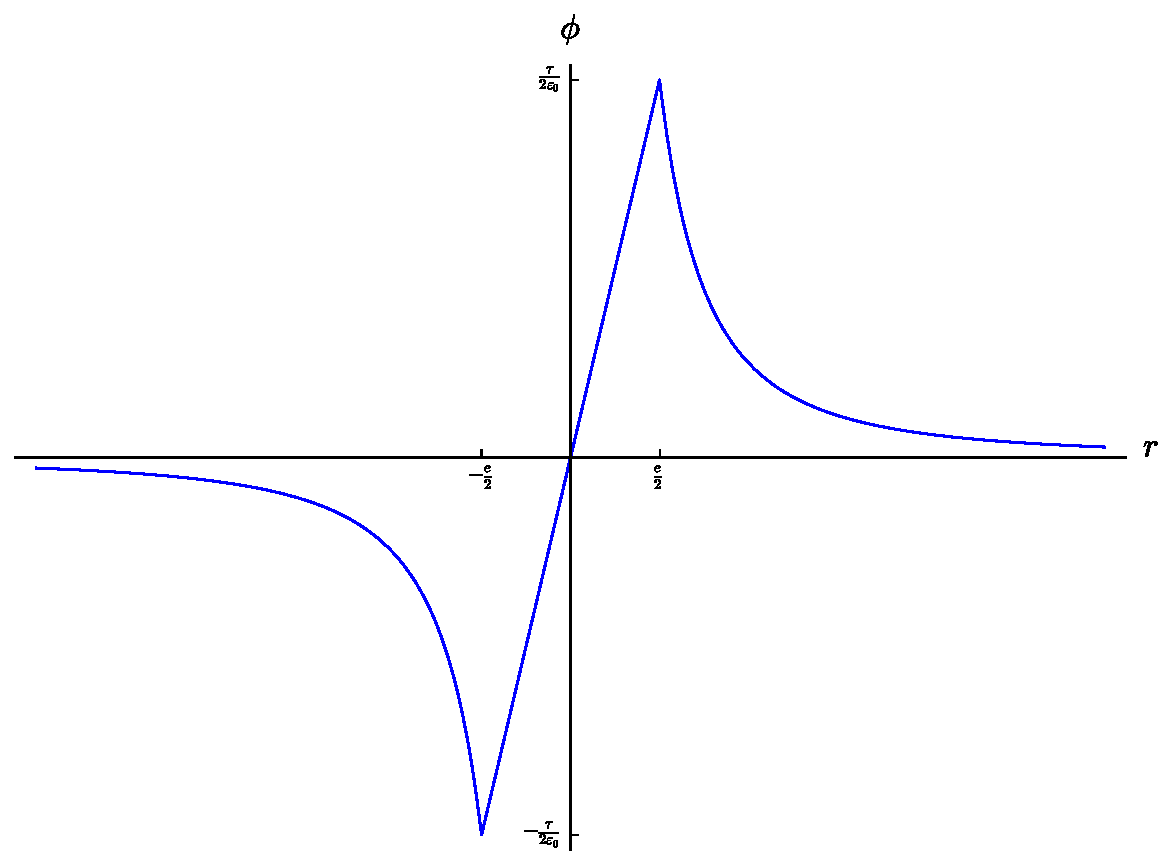
\includegraphics[width=1\linewidth]{electromagnetismo_2018_10_16_6}
\par\end{center}

El eje horizontal representa la distancia con signo al centro de ambas
placas. Es decir, la capa dipolar se sitúa entre ${\displaystyle r=-\frac{e}{2}}$
y ${\displaystyle r=\frac{e}{2}}$. En $r=-\infty$ el ángulo sólido
es $0$ y justo al lado de la distribución (${\displaystyle r=-\frac{e}{2}}$)
el ángulo sólido es $2\pi$; luego, justo en el borde de la capa,
el potencial vale ${\displaystyle -\frac{\tau}{2\varepsilon_{0}}}$.
Al otro lado de la capa dipolar (${\displaystyle r=\frac{e}{2}}$)
el ángulo sólido vale $-2\pi$ y el potencial ${\displaystyle \frac{\tau}{2\varepsilon_{0}}}$.
En $r=\infty$ el ángulo sólido se hace cero.
\end{rem}
%
\begin{rem}
Nótese que el ángulo sólido cambia de signo al pasar de un lado al
otro de la capa dipolar.
\begin{center}
\includegraphics[width=0.6\linewidth]{electromagnetismo_2018_10_19_2}
\par\end{center}

\end{rem}
\begin{prop}
El campo eléctrico generado por una capa dipolar con $\tau$ tal que
$\vec{\nabla}\tau=\vec{0}$ es:

\[
\vec{E}=\frac{\tau}{4\pi\varepsilon_{0}}\oint_{C}\frac{d\vec{l}\times\vec{r}}{r^{3}}
\]
donde la integral se realiza a través de la curva $C$ que delimita
la superficie de la capa dipolar.
\end{prop}
\begin{proof}
Por la proposición \vref{prop:PhiCapaDipolar}, tenemos:
\[
\phi\left(\vec{R}\right)=\frac{-\tau}{4\pi\varepsilon_{0}}\Omega
\]
Por la definición \vref{def:PhiEl=0000E9ctrico}, sabemos que el campo
eléctrico va a ser:

\[
\vec{E}=-\vec{\nabla}\phi
\]
Por tanto, por la regla del producto:

\[
\vec{E}=-\vec{\nabla}\left(-\frac{\tau}{4\pi\varepsilon_{0}}\Omega\right)=-\vec{\nabla}\left(-\frac{\tau}{4\pi\varepsilon_{0}}\right)\Omega+\frac{\tau}{4\pi\varepsilon_{0}}\vec{\nabla}\Omega
\]
Como ${\displaystyle \frac{1}{4\pi\varepsilon_{0}}}$ es una constante:

\[
\vec{E}=\frac{\Omega}{4\pi\varepsilon_{0}}\vec{\nabla}\tau+\frac{\tau}{4\pi\varepsilon_{0}}\vec{\nabla}\Omega
\]
 Ahora, como por hipótesis es $\vec{\nabla}\tau=\vec{0}$, la expresión
anterior queda:

\[
\vec{E}=\frac{\tau}{4\pi\varepsilon_{0}}\vec{\nabla}\Omega
\]
Para ver cuánto cambia el ángulo sólido, vamos a hacer el siguiente
dibujo:
\begin{center}
\includegraphics[width=0.55\linewidth]{electromagnetismo_2018_10_22_2}
\par\end{center}

Así, podemos ver que lo que cambia el ángulo sólido cuando el punto
de referencia se mueve $\vec{\delta}$ es equivalente a que el punto
de referencia no se mueva, pero que la capa dipolar se desplace $-\vec{\delta}$.
En el plano, podemos ver que la variación del ángulo sólido es sumar
la <<parte nueva>> y restar <<la parte que desaparece>>; gráficamente
tendríamos:
\begin{center}
\includegraphics[width=0.65\linewidth]{electromagnetismo_2018_10_22_3}
\par\end{center}

De manera que:

\[
d\Omega=\iint_{S}\frac{\left(-\vec{r}\right)\cdot d\vec{S}}{r^{3}}
\]
Como $d\vec{S}=-\vec{\delta}\times d\vec{l}$:

\[
d\Omega=\oint_{C}-\frac{\vec{r}}{r^{3}}\cdot\left(-\vec{\delta}\times d\vec{l}\right)=\oint_{C}\frac{\vec{r}\cdot\left(d\vec{l}\times\vec{\delta}\right)}{r^{3}}=\oint_{C}\frac{\left(d\vec{l}\times\vec{r}\right)\cdot\vec{\delta}}{r^{3}}=\left(\oint_{C}\frac{d\vec{l}\times\vec{r}}{r^{3}}\right)\cdot\vec{\delta}
\]

Por otra parte, por la regla de la cadena:

\[
d\Omega=\left(\vec{\nabla}\Omega\right)\cdot\vec{\delta}
\]
Hemos obtenido dos expresiones diferentes para $d\Omega$, así que
ambas deben ser iguales:

\[
\left(\oint_{C}\frac{d\vec{l}\times\vec{r}}{r^{3}}\right)\cdot\vec{\delta}=\left(\vec{\nabla}\Omega\right)\cdot\vec{\delta}
\]

Ahora, por regla general, dados cuatro vectores $\vec{A},\vec{B},\vec{C}$
y $\vec{D}$ que cumplen $\begin{matrix}\vec{A}=\vec{B}\cdot\vec{C}\\
\vec{A}=\vec{D}\cdot\vec{C}
\end{matrix}$ no es necesario que $\vec{B}=\vec{D}.$ Sin embargo, en nuestro caso
dado que la igualdad debe cumplirse para cualquier vector $\vec{\delta}$,
forzosamente debe ser:

\[
\vec{\nabla}\Omega=\oint_{C}\frac{d\vec{l}\times\vec{r}}{r^{3}}
\]
Y en consecuencia:

\[
\vec{E}=\frac{\tau}{4\pi\varepsilon_{0}}\oint_{C}\frac{d\vec{l}\times\vec{r}}{r^{3}}
\]
\end{proof}

\chapter{Medios dieléctricos}

\thispagestyle{newchapter}

\section{Introducción}

En la naturaleza aparecen varias estructuras polarizadas como por
ejemplo una red de átomos de carbono en el que uno de dichos átomos
ha sido sustituido por uno de nitrógeno:
\begin{center}
\includegraphics[width=0.55\linewidth]{electromagnetismo_2018_10_22_5}
\par\end{center}

También, al introducir un átomo neutro (como un gas noble) en un campo
eléctrico los electrones cambian sus disposición en torno al núcleo:
\begin{center}
\includegraphics[width=1\linewidth]{electromagnetismo_2018_10_22_6}
\par\end{center}

\section{Polarización dieléctrica}
\begin{assumption}
Supondremos que en los medios dieléctricos no hay cargas libres, en
el sentido de que las cargas no pueden trasladarse, aunque sí rotar.
Dicho de otra forma, la posición de todas las partículas está fija.
\end{assumption}
\begin{defn}
Llamamos \textbf{sustancias polares} a aquellas que, en ausencia de
campos eléctricos externos, presentan momento dipolar. Las sustancias
que no cumplen la condición anterior se llaman \textbf{sustancias
apolares} o \textbf{sustancias no polares}.
\end{defn}
Por ejemplo, la molécula de agua es una sustancia polar:
\begin{center}
\includegraphics[width=0.7\linewidth]{electromagnetismo_2018_10_22_7}
\par\end{center}

De esta forma, en un vaso de agua, en general, al estar los dipolos
distribuidos aleatoriamente, el momento dipolar resultante es nulo
(o casi nulo). Sin embargo, si sometemos las moléculas de agua a un
campo eléctrico, todas se orientan en la dirección de dicho campo
eléctroestático:
\begin{center}
\includegraphics[width=0.5\linewidth]{electromagnetismo_2018_10_22_8}
\par\end{center}
\begin{defn}
Llamamos \textbf{polarización por orientación} al cambio de orientación
que sufre una sustancia polar al verse afectada por un campo eléctrico
externo.
\begin{center}
\includegraphics[width=0.7\linewidth]{electromagnetismo_2018_10_22_9}
\par\end{center}

\end{defn}
%
\begin{defn}
Llamamos \textbf{polarización por deformación} al vector:

\[
\vec{p}=q\cdot\vec{d}
\]
donde $\vec{d}$ es el vector que une los centros de carga negativa
y positiva.
\end{defn}
Un ejemplo de polarización por deformación es:
\begin{center}
\includegraphics[width=0.8\linewidth]{electromagnetismo_2018_10_22_10}
\par\end{center}
\begin{rem}
La polarización por deformación sólo juega un papel importante en
las sustancias no polares, pues si bien existe la polarización por
deformación en las sustancias polares, ésta es despreciable frente
a la polarización por orientación.
\end{rem}
%
\begin{rem}
Nótese que la temperatura influye en el grado de polarización.
\end{rem}
\begin{conclusion}
~

\begin{center}%
\begin{tabular}{|c|c|c|}
\hline 
Sustancia & ¿Presenta momento dipolar en asuencia de campo eléctrico externo? & Polarización por\tabularnewline
\hline 
\hline 
polar & Sí & orientación\tabularnewline
\hline 
no polar & No & deformación\tabularnewline
\hline 
\end{tabular}\end{center}
\end{conclusion}
\begin{defn}
Llamamos \textbf{vector polarización} a:

\[
\vec{P}:=\alpha\vec{E}
\]
donde $\alpha\in\mathbb{R}$ es la polarizabilidad.
\end{defn}

\section{Campo en el interior de un dieléctrico}
\begin{defn}
Llamamos \textbf{reducción al vacío} al proceso de sustituir una distribución
de dipolos por una densidad volumétrica y superficial de carga equivalentes.
\end{defn}
\begin{prop}
Tener un medio material relleno de dipolos es equivalente a tener
unas $\sigma_{b}$ y $\rho_{b}$ equivalentes, donde:

\[
\left\{ \begin{matrix}\sigma_{b}=\vec{P}\cdot\hat{n}\\
\rho_{b}=-\vec{\nabla}\cdot\vec{P}
\end{matrix}\right.
\]
Es decir, las siguientes dos situaciones son equivalentes.
\begin{center}
\includegraphics[width=0.7\linewidth]{electromagnetismo_2018_10_23_1}\includegraphics[width=0.3\linewidth]{electromagnetismo_2018_10_23_2}
\par\end{center}

\end{prop}
\begin{proof}
Se hace por reducción al vacío.
\end{proof}
\begin{cor}
Recordando la proposición \vref{prop:PhiEDistDipolo}, el potencial
y el campo generados por un dieléctrico (en ausencia de cargas reales
(libres {[}no emparejadas{]}) deben ser:

\[
\phi\left(\vec{R}\right)=\frac{1}{4\pi\varepsilon_{0}}\left[\oiint_{S'}\frac{\sigma_{b}}{r}dS'+\iiint_{V'}\frac{\rho_{b}}{r}dV'\right]
\]

\[
\vec{E}\left(\vec{R}\right)=\frac{1}{4\pi\varepsilon_{0}}\left[\oiint_{S'}\frac{\sigma_{b}\hat{r}}{r^{2}}dS'+\iiint_{V'}\frac{\rho_{b}\hat{r}}{r^{2}}dV'\right]
\]

En el caso en que además de carga equivalente hubiera cargas libres,
por el principio de superposición, tenemos:

\[
\phi\left(\vec{R}\right)=\frac{1}{4\pi\varepsilon_{0}}\left[\oiint_{S'}\frac{\sigma_{b}+\sigma_{f}}{r}dS'+\iiint_{V'}\frac{\rho_{b}+\rho_{f}}{r}dV'\right]
\]

\[
\vec{E}\left(\vec{R}\right)=\frac{1}{4\pi\varepsilon_{0}}\left[\oiint_{S'}\frac{\left(\sigma_{b}+\sigma_{f}\right)\hat{r}}{r^{2}}dS'+\iiint_{V'}\frac{\left(\rho_{b}+\rho_{f}\right)\hat{r}}{r^{2}}dV'\right]
\]
donde con $f$ denotamos free (libre, en inglés).
\end{cor}

\section{Vector desplazamiento eléctrico}
\begin{defn}
\label{def:D}Llamamos \textbf{vector de desplazamiento eléctrico}
a:

\[
\vec{D}:=\varepsilon_{0}\vec{E}+\vec{P}
\]
\end{defn}
\begin{thm}[Teorema de Gauss generalizado (forma diferencial)]
\label{thm:GaussGeneralizadoDiferencial}

Las fuentes del desplazamiento eléctrico son las cargas reales (las
cargas libres). Es decir, la divergencia del vector desplazamiento
eléctrico $\vec{D}$ evaluada en un punto $\vec{R}$ coincide con
el valor de la función densidad de carga libre evaluada en dicho punto
$\vec{R}$.

\[
\vec{\nabla}\cdot\vec{D}\left(\vec{R}\right)=\rho_{f}\left(\vec{R}\right)
\]
\end{thm}
\begin{proof}
Por el teorema de Gauss en forma diferencial (ver teorema \vref{thm:GaussDiferencial})
tenemos:

\[
\vec{\nabla}\cdot\vec{E}\left(\vec{R}\right)=\frac{\rho_{\text{total}}\left(\vec{R}\right)}{\varepsilon_{0}}=\frac{\rho_{b}\left(\vec{R}\right)+\rho_{f}\left(\vec{R}\right)}{\varepsilon_{0}}
\]
Por otro lado, habíamos dicho que:

\[
\varepsilon_{0}\vec{\nabla}\cdot\vec{E}=-\vec{\nabla}\cdot\vec{P}+\rho_{f}\Leftrightarrow\varepsilon_{0}\vec{\nabla}\cdot\vec{E}+\vec{\nabla}\cdot\vec{P}=\rho_{f}
\]
Ahora, como la divergencia es un operador lineal, lo anterior es equivalente
a:

\[
\vec{\nabla}\cdot\left(\underbrace{\varepsilon_{0}\vec{E}+\vec{P}}_{=\vec{D}}\right)=\rho_{f}
\]
\end{proof}
\begin{thm}[Teorema de Gauss generalizado (forma integral)]
\label{thm:GaussGeneralizado}

La integral del vector desplazamiento eléctrico a lo largo de una
superficie cerrada es igual a la carga libre encerrada en dicha superficie.

\[
\oiint_{S}\vec{D}\cdot d\vec{S}=Q_{f}
\]
\end{thm}
\begin{proof}
Partimos de:
\[
\oiint_{S}\vec{D}\cdot d\vec{S}
\]
Por el teorema de la divergencia (ver teorema \vref{thm:Divergencia}),
tenemos:
\[
\oiint_{S}\vec{D}\cdot d\vec{S}=\iiint_{V}\vec{\nabla}\cdot\vec{D}dV
\]
Y, por el teorema de Gauss generalizado en forma diferencial (ver
teorema \vref{thm:GaussGeneralizadoDiferencial}), llegamos a:
\[
\iiint_{V}\vec{\nabla}\cdot\vec{D}dV=\iiint_{V}\rho_{f}dV=Q_{f}
\]
\end{proof}
\begin{example}
Tenemos un condensador con un dieléctrico:
\begin{center}
\includegraphics[width=0.4\linewidth]{electromagnetismo_2018_10_23_3}
\par\end{center}

\textcolor{red}{¿Hay algo más que decir aquí?}
\end{example}
\begin{prop}
Sea $\vec{D}$ el vector desplazamiento eléctrico y $\vec{P}$ el
vector polarización. Entonces, sus rotacionales son iguales, siempre
que el campo $\vec{E}$ sea conservativo.

\[
\vec{\nabla}\times\vec{D}=\vec{\nabla}\times\vec{P}
\]
\end{prop}
\begin{proof}[Demostración{*} (No entra)]
 Por la definición del vector desplazamiento eléctrico (ver definición
\vref{def:D}), tenemos:

\[
\vec{\nabla}\times\vec{D}=\vec{\nabla}\times\left(\varepsilon_{0}\vec{E}+\vec{P}\right)
\]
Como el producto vectorial es distributivo respecto a la suma y es
homogéneo de grado 1:

\[
\vec{\nabla}\times\vec{D}=\varepsilon_{0}\vec{\nabla}\times\vec{E}+\vec{\nabla}\times\vec{P}
\]
Como el campo eléctrico es conservativo por hipótesis, por el corolario
\vref{cor:Campo El=0000E9ctrico Cons}, es $\vec{\nabla}\times\vec{E}=\vec{0}$,
de forma que obtenemos:

\[
\vec{\nabla}\times\vec{D}=\vec{\nabla}\times\vec{P}
\]
\end{proof}
\begin{rem}
En general, el rotacional del desplazamiento eléctrico será cero,
pues para conseguir que el rotacional de la densidad de polarización
sea no nulo hace falta recurrir a materiales artificiales como metamateriales
o materiales zurdos.
\end{rem}

\section{Constante dieléctrica y susceptibilidad}
\begin{defn}
\label{def:SuceptibilidadElectrica}En un medio sin polarización permanente,
llamamos \textbf{susceptibilidad eléctrica} al factor adimensional
$\chi$ tal que:

\[
\vec{P}=\varepsilon_{0}\chi\vec{E}
\]
La susceptibilidad eléctrica puede no ser constante. También puede
ser un escalar o un tensor $0,2$ (una matriz), como veremos más adelante:
\end{defn}
%
\begin{defn}
\label{def:epsilon}Llamamos \textbf{permitividad eléctrica de un
medio} a:

\[
\varepsilon:=\varepsilon_{0}\left(1+\chi\right)
\]
\end{defn}
\begin{prop}
\label{prop:DepsilonE}En ausencia de polarización permanente, el
vector desplazamiento eléctrico puede expresarse como:

\[
\vec{D}=\varepsilon_{0}\vec{E}+\varepsilon_{0}\chi\vec{E}=\varepsilon\vec{E}
\]
donde $\varepsilon$ es la permitividad eléctrica del medio.
\end{prop}
\begin{proof}
Por la definición \vref{def:D}, tenemos:

\[
\vec{D}=\varepsilon_{0}\vec{E}+\vec{P}
\]
Ahora, por la definición \vref{def:SuceptibilidadElectrica} lo anterior
se puede expresar como:

\[
\vec{D}=\varepsilon_{0}\vec{E}+\varepsilon_{0}\chi\vec{E}=\varepsilon_{0}\left(1+\chi\right)\vec{E}
\]
Por último, por la definición \vref{def:epsilon}:

\[
\vec{D}=\varepsilon\vec{E}
\]
\end{proof}
\begin{defn}
Llamamos \textbf{permitividad relativa de un medio} al cociente:

\[
\varepsilon_{r}:=\frac{\varepsilon}{\varepsilon_{0}}=1+\chi
\]
\end{defn}
\begin{fact}
En cualquier medio natural se da:

\[
\chi\ge0
\]
Sólo en materiales artificiales se puede conseguir $\chi<0$.
\end{fact}

\section{L.H.I. (Materiales lineales homogéneos e isótropos)}

Aquí tenemos el valor de la permitividad relativa para varios medios:
\begin{center}
\begin{tabular}{|c|c|}
\hline 
Material & $\varepsilon_{r}$\tabularnewline
\hline 
\hline 
vacío & $1$\tabularnewline
\hline 
aire & $1,006$\tabularnewline
\hline 
teflón & $2,1$\tabularnewline
\hline 
parafina & $2,1$\tabularnewline
\hline 
poliestireno & $2,7$\tabularnewline
\hline 
nylon & $3,5$\tabularnewline
\hline 
cuarzo & $5$\tabularnewline
\hline 
amoníaco & $22$\tabularnewline
\hline 
metanol & $34$\tabularnewline
\hline 
glicerina & $50$\tabularnewline
\hline 
agua & $81$\tabularnewline
\hline 
titanato de bario ($\text{Ba}\text{Ti}\text{O}_{3}$) (ferroeléctrico) & $1200-1500$\tabularnewline
\hline 
\end{tabular}
\par\end{center}
\begin{defn}
Llamamos medio \textbf{isótropo} a aquel en el que el vector polarización
y el vector campo eléctrico son paralelos en todo momento:

\[
\vec{P}\parallel\vec{E}
\]

Análogamente, llamamos medios \textbf{anisótropos} a aquellos en los
que $\vec{P}\nparallel\vec{E}$.
\begin{center}
\includegraphics[width=0.3\linewidth]{electromagnetismo_2018_10_23_4}
\par\end{center}

La susceptibilidad sería en este caso un tensor (una matriz $3\times3$):
$\chi=\left(\begin{matrix}\chi_{11} & \chi_{12} & \chi_{13}\\
\chi_{21} & \chi_{22} & \chi_{23}\\
\chi_{31} & \chi_{32} & \chi_{33}
\end{matrix}\right)$
\end{defn}
%
\begin{defn}
Llamamos medios \textbf{lineales} a aquellos en los que la susceptibilidad
no depende del campo eléctrico:

\[
\chi\neq\mathfrak{F}\left(\vec{E}\right)
\]

Análogamente, llamamos medios \textbf{no lineales} a aquellos en los
que $\chi=\mathfrak{F}\left(\vec{E}\right)$.
\end{defn}
%
\begin{defn}
Llamamos medios \textbf{homogéneos} a aquellos en los que la susceptibilidad
no depende de la posición:

\[
\chi\neq\mathfrak{F}\left(\vec{R}\right)
\]

Análogamente, llamamos medios \textbf{no homogéneos} a aquellos en
los que $\chi=\mathfrak{F}\left(\vec{R}\right)$.
\end{defn}

\section{Condiciones frontera entre dos medios dieléctricos}

\subsection{Componente normal}
\begin{prop}
\label{prop:Dn}En la frontera entre dos medios dieléctricos se cumple
que la resta de las componentes normales de los vectores desplazamiento
eléctrico es igual a la densidad de carga libre en la superficie de
contacto entre ambos dieléctricos.

\[
D_{2_{n}}-D_{1_{n}}=\left[\sigma_{f}\right]_{S}
\]
\begin{center}
\includegraphics[width=1\linewidth]{electromagnetismo_2018_10_24_3}
\par\end{center}

\end{prop}
\begin{proof}
Nuestra situación es la siguiente:
\begin{center}
\includegraphics[width=1\linewidth]{electromagnetismo_2018_10_24_1}
\par\end{center}

Es decir, Tenemos una \textit{pill-box} (<<caja de pastillas>>).
\begin{center}
\includegraphics[width=0.5\linewidth]{electromagnetismo_2018_10_24_2}
\par\end{center}

Por el teorema de Gauss generalizado (ver teorema \vref{thm:GaussGeneralizado}),
tenemos:

\[
\oiint_{S}\vec{D}\cdot d\vec{S}=Q_{\text{real}}=\iint_{\text{tapa superior}}\vec{D}\cdot d\vec{S}+\iint_{\text{tapa inferior}}\vec{D}\cdot d\vec{S}+\iint_{\text{superficie lateral}}\vec{D}\cdot d\vec{S}=
\]

\[
=\iint_{S_{2}}\vec{D}_{2}\cdot d\vec{S}_{2}+\iint_{S_{1}}\vec{D}_{1}\cdot d\vec{S}_{1}+0
\]
Lo anterior se debe a que el valor de la integral a lo largo de la
superficie lateral tiende a cero cuando la altura transversal tiende
a cero.

A continuación, tomamos un $\hat{n}$ tal que $d\vec{S}_{2}=dS_{2}\hat{n}$
y $d\vec{S}_{1}=dS_{1}\left(-\hat{n}\right)$, de forma que:

\[
\iint_{S_{2}}\vec{D}_{2}\cdot d\vec{S}_{2}+\iint_{S_{1}}\vec{D}_{1}\cdot d\vec{S}_{1}=\iint_{S_{2}}D_{2_{n}}dS_{2}-\iint_{S_{1}}D_{1_{n}}dS_{1}
\]
El signo menos viene de:

\[
\vec{D}_{1}\cdot d\vec{S}_{1}=\vec{D}_{1}\left(-\hat{n}\right)dS_{1}=-D_{1n}dS_{1}
\]

Por otra parte, como podemos expresar $Q_{\text{real}}=Q_{f}=\iint_{S}\sigma_{f}dS$,
llegamos a:

\[
\iint_{S}\vec{D}\cdot d\vec{S}=\iint_{S}\sigma_{f}dS
\]
En consecuencia, haciendo tender la altura transversal a cero, $S_{1}=S_{2}=S$,
por lo que obtenemos:

\[
\iint_{S}D_{2_{n}}dS-\iint_{S}D_{1_{n}}dS=\iint_{S}\sigma_{f}dS
\]
De esta forma, al ser la suma de las integrales la integral de la
suma:

\[
\iint_{S}\left(D_{2_{n}}-D_{1_{n}}-\sigma_{f}\right)dS=0
\]
Como este argumento debe cumplirse para cualquier superficie sobre
la que apliquemos el teorema de Gauss, necesariamente:
\[
D_{2_{n}}-D_{1_{n}}=\left[\sigma_{f}\right]_{S}
\]
\end{proof}
\begin{cor}
\label{cor:CondFrontera sigma_f=00003D0}Si en la frontera entre dos
medios dieléctricos no hay carga libre, entonces las componentes normales
a la superficie del vector desplazamiento eléctrico serán iguales
en ambos medios dieléctricos; es decir, si $\left[\sigma_{f}\right]_{S}=0$:
\[
D_{2_{n}}=D_{1_{n}}
\]
\end{cor}
\begin{proof}
Se obtiene trivialmente sustituyendo $\left[\sigma_{f}\right]_{S}=0$
en el enunciado de la proposición \vref{prop:Dn}.
\end{proof}
\begin{cor}
\label{cor:Cond Frontera E n}La proposición \vref{prop:Dn} expresada
en función de los campos eléctricos, queda:

\[
\varepsilon_{2}E_{2_{n}}-\varepsilon_{1}E_{1_{n}}=\sigma_{f}
\]
y el caso particular $\sigma_{f}=0$:

\[
\varepsilon_{2}E_{2_{n}}=\varepsilon_{1}E_{1_{n}}
\]
\end{cor}
\begin{proof}
Se obtiene trivialmente al aplicar la definición \vref{def:D} en
la proposición \vref{prop:Dn} y en el corolario \vref{cor:CondFrontera sigma_f=00003D0}.
\end{proof}

\subsection{Componente tangencial}
\begin{prop}
\label{prop:Et}En la frontera de dos medios cualesquiera, siempre
que el campo eléctrico sea conservativo en un entorno de la superficie
de contacto de ambos medios, se cumple que las componentes tangenciales
del campo eléctrico son iguales en la superficie de contacto.

\[
E_{1_{t}}=E_{2_{t}}
\]
\end{prop}
\begin{proof}
Como el campo eléctrico es conservativo por hipótesis, por el corolario
\vref{cor:Campo El=0000E9ctrico Cons}, se cumple:

\[
\vec{\nabla}\times\vec{E}=\vec{0}
\]
En consecuencia, por el teorema de Stokes (\vref{thm:Stokes}):

\[
0=\iint_{S}\left(\vec{\nabla}\times\vec{E}\right)\cdot d\vec{S}=\oint_{C}\vec{E}\cdot d\vec{l}=\int_{\left(1\right)}\vec{E}\cdot\underbrace{d\vec{l}}_{=dl_{1}\hat{t}}+\int_{\left(3\right)}\vec{E}\cdot d\vec{l}+\int_{\left(2\right)}\vec{E}\cdot\underbrace{d\vec{l}}_{=dl_{2}\left(-\hat{t}\right)}+\int_{\left(4\right)}\vec{E}\cdot d\vec{l}
\]

Gráficamente, hemos hecho lo siguiente:
\begin{center}
\includegraphics[width=0.7\linewidth]{electromagnetismo_2018_10_24_4}
\par\end{center}

De nuevo, si hacemos tender la altura del rectángulo a cero, las integrales
en los tramos $\left(3\right)$ y $\left(4\right)$ van a tender a
cero. Luego, obtenemos:

\[
\vec{E}_{1}\cdot d\vec{l}_{1}=E_{1_{t}}\cdot dl_{1}=E_{1_{t}}dl
\]

\[
\vec{E}_{2}\cdot d\vec{l}_{2}=-\vec{E}_{2}\cdot\hat{t}dl_{2}=-E_{2_{t}}dl
\]
En consecuencia:

\[
\int E_{1_{t}}dl-\int E_{2_{t}}dl=0\Leftrightarrow\int\left(E_{1_{t}}-E_{2_{t}}\right)dl=0
\]
Como este argumento funciona para cualquier espira que escojamos,
debe ser:
\[
E_{1_{t}}-E_{2_{t}}=0\Leftrightarrow E_{1_{t}}=E_{2_{t}}
\]
\end{proof}
\begin{cor}
En función del vector desplazamiento eléctrico el enunciado de la
proposición \vref{prop:Et} queda:

\[
\frac{D_{1_{t}}}{\varepsilon_{1}}=\frac{D_{2_{t}}}{\varepsilon_{2}}
\]
\end{cor}
\begin{proof}
Se obtiene trivialmente al aplicar la definición de vector desplazamiento
eléctrico (ver definición \vref{def:D}) a la proposición \vref{prop:Et}.
\end{proof}

\chapter{Sistemas de conductores}

\thispagestyle{newchapter}

\section{Curiosidades introductorias}

Comprender los conductores nos permitirá en el futuro examinar el
comportamiento de metales, plasmas, semiconductores y gases ionizados.
Por ejemplo:
\begin{center}
\includegraphics[width=1\linewidth]{electromagnetismo_2018_10_26_1}
\par\end{center}

\begin{center}
\includegraphics[width=1\linewidth]{electromagnetismo_2018_10_26_2}
\par\end{center}

Como la masa de cualquier ion es mucho mayor que la masa de un electrón,
el cátodo es el que recibe el mayor aporte de energía. Por eso, en
la práctica es preciso refrigerar el cátodo y reforzarlo para que
no se deforme.

\section{Equilibrio electroestático (propiedades de conductores)}
\begin{defn}
Decimos que un objeto se encuentra en \textbf{equilibrio electrostático}
cuando la suma de las fuerzas que actúan sobre cada una de sus cargas
es nula; es decir, si sus cargas no se mueven.
\end{defn}
\begin{prop}
\label{prop:E=00003D0 IntConductor}El campo eléctrico en un conductor
(exceptuando su superficie) en condiciones de equilibrio electroestático
es nulo.

\[
\vec{E}=\vec{0}
\]
\end{prop}
\begin{proof}
Recordemos que nos encontramos en condiciones de electroestática (por
hipótesis). Usaremos reducción al absurdo. Supongamos que $\vec{E}\neq\vec{0}$
en el conductor, entonces, una carga que se encuentre dentro del conductor
sufrirá una fuerza $\vec{F}=q\vec{E}\Rightarrow\vec{a}\neq\vec{0}$,
luego la carga sufrirá una aceleración y se moverá. En consecuencia
no nos encontramos en condiciones de equilibrio electroestático, pero
habíamos supuesto que sí que estábamos en dicha situación; hemos llegado
a un absurdo.
\end{proof}
\begin{cor}
\label{cor:Cond Equipotencial}Un conductor es equipotencial, es decir,
el potencial de un conductor (también en su superficie) es constante.

\[
\phi=\text{cte}
\]
\end{cor}
\begin{proof}
Para cualquier trayectoria entre dos puntos $A$ y $B$ dentro de
un conductor se da:
\begin{center}
\includegraphics[width=0.5\linewidth]{electromagnetismo_2018_10_26_3}\includegraphics[width=0.5\linewidth]{electromagnetismo_2018_10_26_5}
\par\end{center}

\[
\phi_{A}-\phi_{B}=-\int_{B}^{A}\vec{E}\cdot d\vec{r}
\]
Como el campo eléctrico es nulo en un conductor:

\[
\int_{B}^{A}\vec{E}\cdot d\vec{r}=0\Rightarrow\phi_{A}-\phi_{B}=0\Leftrightarrow\phi_{A}=\phi_{B}
\]
Ahora bien, en la superficie del conductor, como el campo eléctrico
existe, su potencial asociado debe ser una función diferenciable y,
en particular, continua. Por tanto, el valor del potencial en la superficie
de un conductor debe ser su valor dentro del conductor.
\end{proof}
\begin{cor}
La carga de un conductor se encuentra siempre en la superficie.
\end{cor}
\begin{proof}
Recordemos el teorema de Gauss (ver teorema \vref{thm:Gauss}):

\[
\vec{\nabla}\cdot\vec{E}=\frac{\rho}{\varepsilon_{0}}
\]
Como en un conductor (exceptuando la superficie) es $\vec{E}=\vec{0}$,
debe ser $\rho=0$. Ahora, como no puede haber cargas en un conductor
(exceptuando la superficie), si éste está cargado, su carga debe situarse
necesariamente en su superficie.
\end{proof}
%
\begin{cor}
\label{cor:Cond D=00003Dsigma_f}La componente normal del vector desplazamiento
eléctrico en el exterior del conductor coincide con la densidad de
carga libre que hay en su superficie. Además, la componente del campo
eléctrico tangente a la superficie del conductor es nula tanto en
el interior como en el exterior del conductor.

\[
D_{2_{n}}=\sigma_{f}
\]

\[
E_{1_{t}}=E_{2_{t}}=0
\]
\end{cor}
\begin{proof}
Aplicando la proposición \vref{prop:Dn}:

\[
D_{2_{n}}-D_{1_{n}}=\sigma_{f}
\]
Ahora, como el campo eléctrico en el interior de un conductor es nulo
$\vec{E}_{1}=\vec{0}$, debe ser, por la definición \vref{def:D},
$D_{1_{n}}=0$. De forma que llegamos a:

\[
D_{2_{n}}=\sigma_{f}
\]
Por otra parte, como el campo en el interior de un conductor es nulo
$\vec{E}_{1}=\vec{0}$, debe ser $E_{1_{t}}=0$. Ahora, por la proposición
\vref{prop:Et}:

\[
0=E_{1_{t}}=E_{2_{t}}
\]
\end{proof}
\begin{cor}
\label{cor:ECondPerp}El campo eléctrico $\vec{E}$ es siempre perpendicular
a la superficie en un conductor.
\end{cor}
\begin{proof}
Se sigue trivialmente del corolario anterior. Si la componente tangencial
del campo eléctrico en la superficie de un conductor es siempre nula,
entonces, únicamente puede tener componente normal.
\end{proof}
\begin{prop}
\label{prop:Apantallamiento}Un conductor con un agujero en su interior
apantalla el interior del campo eléctrico que halla en su exterior.
Es decir, si no hay cargas en dicho agujero, deber ser $\vec{E}=\vec{0}$
en el agujero, independientemente del campo que haya fuera.
\end{prop}
\begin{proof}
Por el teorema de Gauss (ver teorema \vref{thm:Gauss}) aplicado a
la superficie interior del conductor $S_{i}$, sabemos:

\[
\oiint_{S_{i}}\vec{E}\cdot d\vec{S}=0\Rightarrow Q_{S_{i}}=0
\]
Bien, ahora tenemos la siguiente situación:
\begin{center}
\includegraphics[width=0.5\linewidth]{electromagnetismo_2018_10_26_6}
\par\end{center}

Como el campo eléctrico es conservativo, por el corolario \vref{cor:Campo El=0000E9ctrico Cons},
debe ser:

\[
\oint_{C}\vec{E}\cdot d\vec{l}=0\Leftrightarrow\underbrace{\int_{A}^{B}\vec{E}\cdot d\vec{l}}_{=0}+\int_{B}^{A}\vec{E}\cdot d\vec{l}=0
\]
El primer término se anula porque, por la proposición \vref{prop:E=00003D0 IntConductor},
es $\vec{E}=\vec{0}$ dentro del conductor. En consecuencia:

\[
\int_{B}^{A}\vec{E}\cdot d\vec{l}=0
\]
Como podemos realizar la integral anterior a lo largo de cualquier
trayectoria que una los puntos $A$ y $B$ a través del hueco interior
del conductor, debe ser:

\[
\vec{E}=\vec{0}
\]
\end{proof}
\begin{rem}
Nótese que el recíproco no es cierto. Si tenemos cargas en el interior
de un conductor, fuera del conductor sí que habrá campo eléctrico.
Se puede comprobar fácilmente mediante la forma integral del teorema
de Gauss (ver teorema \vref{thm:Gauss}).
\begin{center}
\includegraphics[width=0.5\linewidth]{electromagnetismo_2018_10_26_7}
\par\end{center}

\end{rem}
%
\begin{rem}
Si tenemos un conductor con cargas en su interior y lo conectamos
a tierra, el conductor apantalla el interior del exterior y el exterior
del interior. Podemos verlo con el ejemplo del cable coaxial. Esto
se debe a que al conectar la superficie a tierra, todo el exceso de
carga se va a tierra y desaparece.
\begin{center}
\includegraphics[width=0.5\linewidth]{electromagnetismo_2018_10_26_8}
\par\end{center}
\end{rem}

\section{Teorema de reciprocidad e identidad de Gauss}
\begin{thm}[Teorema de reciprocidad]
\label{thm:Reciprocidad}Sean $\left(1\right)$ y $\left(2\right)$
dos estados de un sistema que contiene $n$ conductores cargados con
carga $q_{1}^{\left(1\right)},\dots,q_{n}^{\left(1\right)}$ respectivamente
en el estado $\left(1\right)$ y con carga $q_{1}^{\left(2\right)},\dots,q_{n}^{\left(2\right)}$
en el estado $\left(2\right)$ y con volumen $V_{1},\dots,V_{n}$.
Dichos conductores se encuentran dentro de un dieléctrico \textbf{l.h.i}
de volumen $T$. Además, sean $\phi_{1}^{\left(1\right)},\dots,\phi_{n}^{\left(2\right)}$
los valores del potencial sobre la superficie de los conductores en
el estado $\left(1\right)$ y sean $\phi_{1}^{\left(2\right)},\dots,\phi_{n}^{\left(2\right)}$
los valores del potencial en la superficie de los conductores en el
estado $\left(2\right)$. Por último, sean $\rho_{f}^{\left(1\right)}$
y $\rho_{f}^{\left(2\right)}$ las funciones densidades de carga \textbf{libre}
del dieléctrico en los estados $\left(1\right)$ y $\left(2\right)$,
respectivamente. Asimismo, sean $\phi^{\left(1\right)}$ y $\phi^{\left(2\right)}$
las funciones potencial en el dieléctrico en los estados $\left(1\right)$
y $\left(2\right)$, respectivamente. Supongamos, también, que el
potencial en la superficie exterior que delimita nuestro dieléctrico
vale cero. Entonces, se cumple:

\[
\iiint_{T-\sum_{j=1}^{n}V_{j}}\left(\phi^{\left(2\right)}\rho_{f}^{\left(1\right)}-\phi^{\left(1\right)}\rho_{f}^{\left(2\right)}\right)dV=\sum_{j=1}^{n}\left(\phi_{j}^{\left(2\right)}q_{j}^{\left(1\right)}-\phi_{j}^{\left(1\right)}q_{j}^{\left(2\right)}\right)
\]
\begin{center}
\includegraphics[width=0.55\linewidth]{electromagnetismo_2018_10_29_1}
\par\end{center}

\end{thm}
\begin{proof}
Como la carga en un conductor está distribuida a lo largo de la superficie,
debe ser:

\begin{equation}
q_{j}^{\left(1\right)}=\oiint_{S_{j}}\sigma_{j}^{\left(1\right)}\cdot d\vec{S}_{j}\label{eq:q_j (1)}
\end{equation}
También, por el corolario \vref{cor:Cond Frontera E n}, sabemos:

\begin{equation}
\frac{\sigma_{j}^{\left(1\right)}}{\varepsilon}=E_{n_{j}}^{\left(1\right)}=-\left(\frac{\partial\phi_{j}^{\left(1\right)}}{\partial\hat{n}_{j}}\right)_{S_{j}}\label{eq:E_n (1)}
\end{equation}
donde $\hat{n}$ es el vector unitario perpendicular a la superficie
del conductor $j$-ésimo que se dirige hacia fuera de dicho conductor.

Recordemos que por el corolario \vref{cor:ECondPerp}, en la superficie
de un conductor no puede haber componente tangencial. De aquí, obtendríamos
una función potencial $\phi^{\left(1\right)}$.

Por ejemplo, en el caso de un condensador, tendríamos:
\begin{center}
\includegraphics[width=0.4\linewidth]{electromagnetismo_2018_10_29_2}
\par\end{center}

\[
\Delta V=\phi_{1}^{\left(1\right)}-\phi_{2}^{\left(1\right)}
\]

\[
\begin{matrix}q_{1}^{\left(1\right)}=Q &  & q_{2}^{\left(1\right)}=-Q\end{matrix}
\]

Volviendo a nuestro caso original, en una situación $\left(2\right)$,
las cargas ahora son $q_{1}^{\left(2\right)},\dots,q_{n}^{\left(2\right)}$.
De nuevo:

\begin{equation}
q_{j}^{\left(2\right)}=\oiint_{S_{j}}\sigma_{j}^{\left(2\right)}dS_{j}\label{eq:q_j(2)}
\end{equation}
y por el corolario \vref{cor:Cond Frontera E n}:

\begin{equation}
\frac{\sigma_{j}^{\left(2\right)}}{\varepsilon}=E_{n_{j}}^{\left(2\right)}=-\left(\frac{\partial\phi_{j}^{\left(2\right)}}{\partial\hat{n}_{j}}\right)_{S_{j}}\label{eq:E_n (2)}
\end{equation}

Al igual que antes, de aquí obtendríamos una función potencial $\phi^{\left(2\right)}$.
Si ahora aplicamos la segunda identidad de Green (ver teorema \vref{thm:Green}):

\[
\iiint_{V}\left(\psi\nabla^{2}\phi-\phi\nabla^{2}\psi\right)dV=\oiint_{S}\left(\psi\frac{\partial\phi}{\partial\hat{n}}-\phi\frac{\partial\psi}{\partial\hat{n}}\right)dS
\]
tomando $\psi=\phi^{\left(1\right)}$ y $\phi=\phi^{\left(2\right)}$,
obtenemos:

\begin{equation}
\iiint_{V}\left[\phi^{\left(1\right)}\nabla^{2}\phi^{\left(2\right)}-\phi^{\left(2\right)}\nabla^{2}\phi^{\left(1\right)}\right]dV=\oiint_{S}\left(\phi^{\left(1\right)}\frac{\partial\phi^{\left(2\right)}}{\partial\hat{n}}-\phi^{\left(2\right)}\frac{\partial\phi^{\left(1\right)}}{\partial\hat{n}}\right)dS\label{eq:Laplace PartialPhi}
\end{equation}

Por otra parte, por la definición \vref{def:PhiEl=0000E9ctrico},
por el teorema de Gauss Generalizado en forma diferencial (ver teorema
\vref{thm:GaussGeneralizadoDiferencial}) y por la proposición \vref{prop:DepsilonE},
tenemos:
\[
\vec{\nabla}\cdot\vec{D}=\rho_{f}\Leftrightarrow\vec{\nabla}\cdot\varepsilon\vec{E}=\rho_{f}\Leftrightarrow\varepsilon\vec{\nabla}\cdot\vec{E}=\rho_{f}\Leftrightarrow-\varepsilon\vec{\nabla}\cdot\vec{\nabla}\phi=\rho_{f}\Leftrightarrow\nabla^{2}\phi=-\frac{\rho_{f}}{\varepsilon}
\]

En consecuencia, \vref{eq:Laplace PartialPhi} es equivalente a:
\[
\iiint_{V}\left[\phi^{\left(1\right)}-\frac{\rho_{f}^{\left(2\right)}}{\varepsilon}-\phi^{\left(2\right)}\left(-\frac{\rho_{f}^{\left(1\right)}}{\varepsilon}\right)\right]dV=\oiint_{S}\left(\phi^{\left(1\right)}\frac{\partial\phi^{\left(2\right)}}{\partial\hat{n}}-\phi^{\left(2\right)}\frac{\partial\phi^{\left(1\right)}}{\partial\hat{n}}\right)dS\Leftrightarrow
\]
\[
\Leftrightarrow\iiint_{V}\left[\phi^{\left(2\right)}\frac{\rho_{f}^{\left(1\right)}}{\varepsilon}-\phi^{\left(1\right)}\frac{\rho_{f}^{\left(2\right)}}{\varepsilon}\right]dV=\oiint_{S}\left(\phi^{\left(1\right)}\frac{\partial\phi^{\left(2\right)}}{\partial\hat{n}}-\phi^{\left(2\right)}\frac{\partial\phi^{\left(1\right)}}{\partial\hat{n}}\right)dS
\]
Haciendo uso de las ecuaciones \vref{eq:E_n (1)} y \vref{eq:E_n (2)},
la expresión anterior se transforma en:
\[
\iiint_{V}\left[\phi^{\left(2\right)}\frac{\rho_{f}^{\left(1\right)}}{\varepsilon}-\phi^{\left(1\right)}\frac{\rho_{f}^{\left(2\right)}}{\varepsilon}\right]dV=\oiint_{S}\left(\phi^{\left(1\right)}\left(-\frac{\sigma_{j}^{\left(2\right)}}{\varepsilon}\right)-\phi^{\left(2\right)}\left(-\frac{\sigma_{j}^{\left(1\right)}}{\varepsilon}\right)\right)dS\Leftrightarrow
\]
\begin{equation}
\Leftrightarrow\iiint_{V}\left[\phi^{\left(2\right)}\frac{\rho_{f}^{\left(1\right)}}{\varepsilon}-\phi^{\left(1\right)}\frac{\rho_{f}^{\left(2\right)}}{\varepsilon}\right]dV=\oiint_{S}\left(\phi^{\left(2\right)}\frac{\sigma_{j}^{\left(1\right)}}{\varepsilon}-\phi^{\left(1\right)}\frac{\sigma_{j}^{\left(2\right)}}{\varepsilon}\right)dS\label{eq:Rho Simga Phi SemiFinal}
\end{equation}

Como en el interior de los conductores no hay cargas libres, podemos
restringir la integral al volumen del dieléctrico menos el volumen
de los conductores. Ahora, recordemos que $T$ es el volumen de todo
el espacio considerado, entonces el volumen del dieléctrico excluyendo
los conductores es:

\[
V=T-\sum_{j=1}^{n}V_{j}
\]

Asimismo, podemos descomponer la integral en superficie en una suma
de integrales a lo largo de las superficies de todos los conductores
más la integral a lo largo de la superficie exterior. Pero el potencial
se anula por hipótesis sobre dicha superficie exterior, luego la integral
también.

\[
\left[\phi^{\left(1\right)}\right]_{S_{\text{exterior}}}=\left[\phi^{\left(2\right)}\right]_{S_{\text{exterior}}}=0\Rightarrow\oiint_{S_{\text{exterior}}}\left[\underbrace{\phi^{\left(2\right)}}_{=0}\frac{\sigma_{j}^{\left(1\right)}}{\varepsilon}-\underbrace{\phi^{\left(1\right)}}_{=0}\frac{\sigma_{j}^{\left(2\right)}}{\varepsilon}\right]dS=0
\]

En consecuencia, la ecuación \vref{eq:Rho Simga Phi SemiFinal} se
transforma en:

\[
\iiint_{T-\sum_{j=1}^{n}V_{j}}\left(\phi^{\left(2\right)}\frac{\rho_{f}^{\left(1\right)}}{\varepsilon}-\phi^{\left(1\right)}\frac{\rho_{f}^{\left(2\right)}}{\varepsilon}\right)dV=\sum_{j=1}^{n}\oiint_{S_{j}}\left[\phi_{j}^{\left(2\right)}\frac{\sigma_{j}^{\left(1\right)}}{\varepsilon}-\phi_{j}^{\left(1\right)}\frac{\sigma_{j}^{\left(2\right)}}{\varepsilon}\right]dS_{j}
\]
donde $\phi_{j}$ es el potencial en la superficie $S_{j}$. Como
nuestro medio es homogéneo, $\varepsilon\neq\mathfrak{F}\left(V\right)$,
podemos sacar el $\varepsilon$ fuera de ambas integrales. Por otra
parte, al ser $\phi_{j}^{\left(1\right)}$ y $\phi_{j}^{\left(2\right)}$
constantes en todos los conductores, podemos escribir la expresión
anterior como:
\[
\frac{1}{\varepsilon}\iiint_{T-\sum_{j=1}^{n}V_{j}}\left(\phi^{\left(2\right)}\rho_{f}^{\left(1\right)}-\phi^{\left(1\right)}\rho_{f}^{\left(2\right)}\right)dV=\frac{1}{\varepsilon}\sum_{j=1}^{n}\left[\phi_{j}^{\left(2\right)}\oiint_{S_{j}}\sigma_{j}^{\left(1\right)}dS_{j}-\phi_{j}^{\left(1\right)}\oiint_{S_{j}}\sigma_{j}^{\left(2\right)}dS_{j}\right]
\]
Por último, multiplicando por $\varepsilon$ a ambos lados y haciendo
uso de las ecuaciones \vref{eq:q_j (1)} y \vref{eq:q_j(2)}, obtenemos:

\[
\iiint_{T-\sum_{j=1}^{n}V_{j}}\left(\phi^{\left(2\right)}\rho_{f}^{\left(1\right)}-\phi^{\left(1\right)}\rho_{f}^{\left(2\right)}\right)dV=\sum_{j=1}^{n}\left(\phi_{j}^{\left(2\right)}q_{j}^{\left(1\right)}-\phi_{j}^{\left(1\right)}q_{j}^{\left(2\right)}\right)
\]
\end{proof}
\begin{cor}[Identidad de Gauss]
Sean $\left(1\right)$ y $\left(2\right)$ dos estados de un sistema
que contiene $n$ conductores cargados con carga $q_{1}^{\left(1\right)},\dots,q_{n}^{\left(1\right)}$
respectivamente en el estado $\left(1\right)$ y con carga $q_{1}^{\left(2\right)},\dots,q_{n}^{\left(2\right)}$
en el estado $\left(2\right)$. Dichos conductores se encuentran dentro
de un dieléctrico \textbf{l.h.i}. Además, sean $\phi_{1}^{\left(1\right)},\dots,\phi_{n}^{\left(2\right)}$
los valores del potencial sobre la superficie de los conductores en
el estado $\left(1\right)$ y sean $\phi_{1}^{\left(2\right)},\dots,\phi_{n}^{\left(2\right)}$
los valores del potencial en la superficie de los conductores en el
estado $\left(2\right)$. Por último, sean $\rho_{f}^{\left(1\right)}=0=\rho_{f}^{\left(2\right)}$
las funciones densidades de carga \textbf{libre} del dieléctrico en
los estados $\left(1\right)$ y $\left(2\right)$, respectivamente.
Supongamos, también, que el potencial en la superficie exterior que
delimita nuestro dieléctrico vale cero. Entonces, se cumple:

\[
\sum_{j=1}^{n}\left(\phi_{j}^{\left(2\right)}q_{j}^{\left(1\right)}-\phi_{j}^{\left(1\right)}q_{j}^{\left(2\right)}\right)=0
\]
\end{cor}
\begin{proof}
Se sigue trivialmente al sustituir $\rho_{f}^{\left(1\right)}=0=\rho_{f}^{\left(2\right)}$
en el teorema \vref{thm:Reciprocidad} y se usa que la integral definida
de cero es cero.
\end{proof}

\subsection{Casos concretos}
\begin{example}
Cuando es $n=1$ en la identidad de Gauss, obtenemos el caso del condensador.

\[
q^{\left(1\right)}\phi^{\left(2\right)}=q^{\left(2\right)}\phi^{\left(1\right)}\Leftrightarrow\frac{q^{\left(1\right)}}{\phi^{\left(1\right)}}=\frac{q^{\left(2\right)}}{\phi^{\left(2\right)}}=\text{cte}:=\text{capacidad del conductor}
\]
\end{example}

\section{Relación entre los potenciales y las cargas}
\begin{defn}
Sea un medio dieléctrico homogéneo de permitividad $\varepsilon$
en el que se encuentran $n$ conductores. Llamamos matriz de \textbf{coeficientes
del potencial} a:

\[
\mathbf{P}\equiv\left(p_{ij}\right):=\left(\begin{matrix}p_{11} & \cdots & p_{1n}\\
\vdots & \ddots & \vdots\\
p_{n1} & \cdots & p_{nn}
\end{matrix}\right)
\]

Cada uno de los componentes de la matriz viene dado por:

\[
p_{ij}:=\frac{1}{4\pi\varepsilon q_{i}q_{j}}\oiint_{S_{i}}\oiint_{S_{j}}\frac{\sigma_{i}\sigma_{j}}{r_{ij}}dS_{i}dS_{j}
\]

donde $q_{i}$ es la carga del conductor $i$, $q_{j}$ es la carga
del conductor $j$, $r_{ij}$ es la distancia que separa ambos conductores,
$S_{i}$ es la superficie exterior del conductor $i$, $S_{j}$ es
la superficie exterior del conductor $j$, $\sigma_{i}$ es la densidad
de carga superficial del conductor $i$ y $\sigma_{j}$ es la densidad
de carga superficial del conductor $j$.

Físicamente, el coeficiente $p_{ji}$ es el potencial que adquiriría
el conductor $j$ cuando todos los conductores están descargados a
excepción del $i$ que posee una carga de un culombio.
\end{defn}
\begin{rem}
Nótese que los $p_{ji}$ no dependen de las cargas, sino únicamente
de la geometría. Esto se debe a que siempre podemos expresar las densidades
de carga superficiales como $\sigma_{i}=q_{i}\cdot f_{i}\left(\vec{R}\right)$
y $\sigma_{j}=q_{j}\cdot f_{j}\left(\vec{R}\right)$ donde las $f_{i}$
y $f_{j}$ son funciones que dependen exclusivamente de la geometría,
devolviendo la distribución relativa de la carga. Nótese también que
$p_{ij}=p_{ji}$, por lo que la matriz $\mathbf{P}$ es simétrica.
\end{rem}
%
\begin{rem}
En la práctica, como los $p_{ji}$ sólo dependen de la geometría,
los podremos calcular para la distribución de cargas que nos sea más
sencilla.
\end{rem}
\begin{defn}
La matriz inversa de la matriz de coeficientes del potencial se llama
matriz de \textbf{coeficientes de influencia de capacidad}.

\[
\mathbf{C}:=\mathbf{P}^{-1}
\]
\end{defn}
\begin{prop}
\label{prop:phi=00003DPQ}Supongamos que tenemos $n$ conductores
en un dieléctrico homogéneo. Sea $\text{\ensuremath{\bm{\Phi}}}=\left(\begin{matrix}\phi_{1}\\
\vdots\\
\phi_{n}
\end{matrix}\right)$ el vector que contiene el valor del potencial sobre la superficie
de cada uno de los conductores. Análogamente, sea $\mathbf{Q}=\left(\begin{matrix}q_{1}\\
\vdots\\
q_{n}
\end{matrix}\right)$ el vector que contiene la carga de cada uno de los conductores. Además,
sea $\mathbf{P}$ la matriz de coeficientes del potencial asociada
a nuestro sistema. Entonces:

\[
\bm{\Phi}=\mathbf{P}\cdot\mathbf{Q}
\]
\begin{center}
\includegraphics[width=0.5\linewidth]{electromagnetismo_2018_10_30_1}
\par\end{center}

\end{prop}
\begin{proof}
Claramente, por cada conductor $i$ se da:
\[
dS_{i}\rightarrow dq=\sigma_{i}dS_{i}
\]
De forma que el diferencial de potencial que el conductor $i$ genera
en el $j$ es: 

\[
d\phi_{ji}=\frac{1}{4\pi\varepsilon}\frac{\sigma_{i}dS_{i}}{r_{ij}}
\]
En consecuencia, el potencial generado en el conductor $j$ debido
al conductor $i$ es:

\[
\phi_{ji}=\oiint_{S_{i}}\frac{1}{4\pi\varepsilon}\frac{\sigma_{i}dS_{i}}{r_{ij}}
\]
Como el dieléctrico es homogéneo, entonces:

\[
\phi_{ji}=\frac{1}{4\pi\varepsilon}\oiint_{S_{i}}\frac{\sigma_{i}dS_{i}}{r_{ij}}
\]
Por consiguiente el potencial en el conductor $j$ es:

\[
\phi_{j}=\sum_{i=1}^{n}\frac{1}{4\pi\varepsilon}\oiint_{S_{i}}\frac{\sigma_{i}dS_{i}}{r_{ij}}
\]

Si multiplicamos y dividimos por $q_{j}=\oiint_{S_{j}}\sigma_{j}dS_{j}$
y, además, también multiplicamos y dividimos por $q_{i}$, llegamos
a:

\[
\phi_{j}=\sum_{i=1}^{n}\underbrace{\frac{1}{4\pi\varepsilon q_{i}q_{j}}\oiint_{S_{i}}\oiint_{S_{j}}\frac{\sigma_{i}\sigma_{j}}{r_{ij}}dS_{i}dS_{j}}_{=p_{ji}}q_{i}=\sum_{i=1}^{n}p_{ji}q_{i}
\]
En consecuencia, podemos escribir la igualdad anterior de la siguiente
forma:

\[
\underbrace{\left(\begin{matrix}\phi_{1}\\
\vdots\\
\phi_{n}
\end{matrix}\right)}_{=\bm{\Phi}}=\underbrace{\left(\begin{matrix}p_{11} & \cdots & p_{1n}\\
\vdots & \ddots & \vdots\\
p_{n1} & \cdots & p_{nn}
\end{matrix}\right)}_{=\mathbf{P}}\underbrace{\left(\begin{matrix}q_{1}\\
\vdots\\
q_{n}
\end{matrix}\right)}_{=\mathbf{Q}}\Leftrightarrow
\]

\[
\Leftrightarrow\bm{\Phi}=\mathbf{P}\cdot\mathbf{Q}
\]
\end{proof}

\section{Influencia total: condensadores}

Supongamos que tenemos dos condensadores:
\begin{center}
\includegraphics[width=0.5\linewidth]{electromagnetismo_2018_10_30_2}\includegraphics[width=0.5\linewidth]{electromagnetismo_2018_10_30_3}
\par\end{center}
\begin{example}
Para el caso de dos conductores, tendríamos:

\[
\left\{ \begin{matrix}\phi_{1}=p_{11}q_{1}+p_{12}q_{2}\\
\phi_{2}=p_{21}q_{1}+p_{22}q_{2}
\end{matrix}\right.
\]

Ahora, si ambas cargas son iguales (pero de signo contrario) $q:=q_{1}=-q_{2}$,
lo anterior se reduce a:

\[
\left\{ \begin{matrix}\phi_{1}=p_{11}q-p_{12}q\\
\phi_{2}=p_{21}q-p_{22}q
\end{matrix}\right.
\]
Si hallamos $\phi_{1}-\phi_{2}$:

\[
\phi_{1}-\phi_{2}=q\left(p_{11}-2p_{12}+p_{22}\right)
\]
Despejando $q$:

\[
q=\frac{\phi_{1}-\phi_{2}}{p_{11}+p_{22}-2p_{12}}
\]

Ahora, definiendo $C:=\frac{1}{p_{11}+p_{22}-2p_{12}}$, obtenemos:

\[
q=C\left(\phi_{1}-\phi_{2}\right)
\]
Utilizando las $c_{ij}$ (las inversas de $p_{ij}$), llegamos a:

\[
\left\{ \begin{matrix}q_{1}=c_{11}\phi_{1}+c_{12}\phi_{2}\\
q_{2}=c_{21}\phi_{1}+c_{22}\phi_{2}
\end{matrix}\right.
\]
Si suponemos $q_{1}=-q_{2}$ y sumamos obtendríamos:

\[
0=\left(c_{11}+c_{21}\right)\phi_{1}+\left(c_{12}+c_{22}\right)\phi_{2}\Leftrightarrow\left\{ \begin{matrix}c_{11}=-c_{21}\\
c_{12}=-c_{22}
\end{matrix}\right.
\]
\end{example}

\chapter{Energía electrostática}

\thispagestyle{newchapter}
\begin{defn}
Llamaremos \textbf{energía electroestática} de un sistema de cargas
puntuales al trabajo necesario para traer todas ellas desde el infinito
una a una.

Para el caso de distribuciones volumétricas de carga en un medio dieléctrico,
la energía electroestática será el trabajo necesario para aumentar
la densidad volumétrica de carga libre $\rho_{f}$ desde la función
nula en todos los puntos hasta la distribución final.
\end{defn}

\section{Energía de un sistema de cargas puntuales}
\begin{prop}
\label{prop:UePuntual}La energía electrostática $U_{e}$ almacenada
en un sistema aislado de $n$ cargas puntuales $\left\{ q_{k}\right\} _{k=1,\dots,n}$
viene dada por:

\[
U_{e}=W_{n}=\frac{1}{2}\sum_{i=1}^{n}q_{i}\sum_{\begin{matrix}j=1\\
i\neq j
\end{matrix}}^{n}\phi_{ij}=\frac{1}{2}\sum_{i=1}^{n}q_{i}\phi_{i}
\]
donde $\phi_{ij}\equiv\phi_{i\leftarrow j}$ es el potencial que crea
la partícula $j$ sobre la $i$ y $\phi_{i}$ es el potencial de la
partícula $i$, es decir: $\phi_{i}={\displaystyle \sum_{j=1}^{n}\phi_{i\leftarrow j}}$.
\end{prop}
\begin{proof}
Podemos suponer, sin pérdida de generalidad, que nuestro sistema de
cargas puntuales se encuentra en el interior de un conductor, ya que
por la proposición \vref{prop:Apantallamiento}, un conductor aísla
el interior del exterior.
\begin{center}
\includegraphics[width=0.5\linewidth]{electromagnetismo_2018_11_7_1}
\par\end{center}

En el interior del mencionado conductor contamos con $n$ cargas puntuales:
\begin{center}
\includegraphics[width=0.45\linewidth]{electromagnetismo_2018_11_7_2}
\par\end{center}

Veamos qué trabajo tenemos que realizar para llevar la $q_{1}$ desde
la superficie del $\infty$ hasta el punto $1$:

\[
w_{1}=0
\]
El trabajo es nulo, pues no tengo ninguna carga en mi sistema todavía.

Ahora, quiero llevar la carga $q_{2}$ al punto $2$:

\[
w_{2}=q_{2}\phi_{2\leftarrow1}\equiv q_{2}\phi_{21}
\]
De manera que el trabajo total para dos cargas es:

\[
W_{2}=w_{1}+w_{2}=q_{2}\phi_{21}=q_{2}\frac{1}{4\pi\varepsilon_{0}}\frac{q_{1}}{r_{12}}=\frac{1}{2}\left(\frac{1}{4\pi\varepsilon_{0}}\frac{q_{1}q_{2}}{r_{12}}+\frac{1}{4\pi\varepsilon_{0}}\frac{q_{1}q_{2}}{r_{12}}\right)
\]
Como $r_{12}=r_{21}$, podemos expresar lo anterior como:

\[
W_{2}=\frac{1}{2}\left(\phi_{21}q_{2}+\phi_{12}q_{1}\right)=\frac{1}{2}\left(q_{1}\phi_{12}+q_{2}\phi_{21}\right)
\]

Ahora, traigo la carga $3$:

\[
w_{3}=q_{3}\phi_{3}=q_{3}\left(\phi_{31}+\phi_{32}\right)
\]
Haciendo lo mismo que antes, obtenemos:
\[
w_{3}=q_{3}\left(\frac{1}{4\pi\varepsilon_{0}}\frac{q_{1}}{r_{13}}+\frac{1}{4\pi\varepsilon_{0}}\frac{q_{2}}{r_{23}}\right)=\frac{1}{2}\left(q_{3}\phi_{31}+q_{1}\phi_{13}+q_{2}\phi_{23}+q_{3}\phi_{32}\right)
\]

\[
w_{3}=\frac{1}{2}\left(q_{3}\phi_{31}+q_{1}\phi_{13}+q_{3}\phi_{32}+q_{2}\phi_{23}\right)
\]
En consecuencia:

\[
W_{3}=\frac{1}{2}\left(q_{1}\phi_{12}+q_{1}\phi_{13}+q_{2}\phi_{21}+q_{2}\phi_{23}+q_{3}\phi_{31}+q_{3}\phi_{32}\right)
\]

De forma, que, en general:

\[
W_{n}=\frac{1}{2}\sum_{i=1}^{n}q_{i}\underbrace{\sum_{\begin{matrix}j=1\\
i\neq j
\end{matrix}}^{n}\phi_{ij}}_{=\phi_{i}}=\frac{1}{2}\sum_{i=1}^{n}q_{i}\phi_{i}=U_{e}
\]
\end{proof}

\section{Energía de una distribución de cargas}
\begin{defn}
\label{def:ue}Llamamos \textbf{densidad de energía electrostática}
de un sistema en un punto $\vec{R}$ a:

\[
u_{e}\left(\vec{R}\right):=\frac{1}{2}\vec{E}\left(\vec{R}\right)\cdot\vec{D}\left(\vec{R}\right)
\]
Sus unidades son ${\displaystyle \left[u_{e}\right]=\frac{\text{J}}{\text{m}^{3}}}$.
\end{defn}
\begin{prop}
\label{prop:Ue}La energía electroestática almacenada en una distribución
de cargas con densidad de carga $\rho\left(\vec{R}'\right)$ y volumen
$V'$ es:

\[
U_{e}=\frac{1}{2}\iiint_{V'}\rho\left(\vec{R}'\right)\phi\left(\vec{R}'\right)dV'=\frac{1}{2}\iiint_{T.E}\vec{E}\cdot\vec{D}\,dV=\iiint_{T.E}u_{e}dV
\]
donde con $T.E$ nos referimos a todo el espacio, es decir, al volumen
$V'$ más todo lo que hay fuera.
\begin{center}
\includegraphics[width=0.45\linewidth]{electromagnetismo_2018_11_7_3}
\par\end{center}

\end{prop}
\begin{proof}
Partimos de la proposición \vref{prop:UePuntual}:

\[
U_{e}=\frac{1}{2}\sum_{i=1}^{n}q_{i}\phi_{i}
\]
Como ahora estamos en un medio continuo, el número de partículas tiende
a infinito, por lo que podemos aproximar la suma por una integral:

\[
U_{e}\approxeq\frac{1}{2}\iiint dq\,\phi_{q}
\]
Como es $dq=\rho\left(\vec{R}'\right)dV'$, podemos expresar lo anterior
como:

\[
U_{e}=\frac{1}{2}\iiint_{V'}\rho\left(\vec{R}'\right)\phi\left(\vec{R}'\right)dV'
\]

Por el teorema de Gauss generalizado (ver teorema \vref{thm:GaussGeneralizadoDiferencial})
$\rho\left(\vec{R}'\right)=\vec{\nabla}\cdot\vec{D}$, de forma que:

\begin{equation}
U_{e}=\frac{1}{2}\iiint_{V'}\rho\left(\vec{R}'\right)\phi\left(\vec{R}'\right)dV'=\frac{1}{2}\iiint_{T.E}\left(\vec{\nabla}\cdot\vec{D}\right)\phi\left(\vec{R}'\right)dV\label{eq:Ue divDPhi}
\end{equation}
Por otra parte, por la regla del producto:

\[
\vec{\nabla}\cdot\left(\phi\vec{D}\right)=\phi\vec{\nabla}\cdot\vec{D}+\vec{D}\cdot\vec{\nabla}\phi\Leftrightarrow
\]

\[
\Leftrightarrow\vec{\nabla}\left(\phi\vec{D}\right)-\vec{D}\cdot\vec{\nabla}\phi=\phi\vec{\nabla}\cdot\vec{D}
\]
En consecuencia, puedo reescribir \vref{eq:Ue divDPhi} como:

\[
U_{e}=\frac{1}{2}\left[\iiint_{T.E}\vec{\nabla}\cdot\left(\phi\vec{D}\right)dV+\iiint_{T.E}\vec{D}\cdot\vec{E}dV\right]
\]
Por el teorema de la divergencia (ver teorema \vref{thm:Divergencia}):

\begin{equation}
U_{e}=\frac{1}{2}\oiint_{S}\phi\vec{D}\cdot d\vec{S}+\frac{1}{2}\iiint_{T.E}\vec{D}\cdot\vec{E}dV\label{eq:Ue DEdV + phiDdS}
\end{equation}
donde $S$ es la superficie que delimita todo el volumen, es decir,
la superficie del infinito $\Sigma_{\infty}$. Si hacemos tender $r\rightarrow\infty$
y observamos el comportamiento de los términos de la primera integral,
obtenemos por desarrollo multipolar ${\displaystyle \phi\sim\frac{1}{r}}$,
${\displaystyle D\sim\frac{1}{r^{2}}}$ y $S\sim r^{2}\Rightarrow dS\sim rdr$.
En consecuencia:

\[
\oiint_{S}\phi\vec{D}\cdot d\vec{S}\sim\int\frac{1}{r}\frac{1}{r^{2}}rdr=\int\frac{1}{r^{2}}dr=-\frac{1}{r}\xrightarrow[r\rightarrow\infty]{}0
\]
cuando $r\rightarrow\infty$. Luego, claramente si $r\rightarrow\infty$
(lo cual se da en la superficie del infinito), entonces $\oiint_{S}\phi\vec{D}\cdot d\vec{S}\rightarrow0$.
Por consiguiente, como el producto escalar es conmutativo, \vref{eq:Ue DEdV + phiDdS}
queda en:

\[
U_{e}=\frac{1}{2}\iiint_{T.E}\vec{E}\cdot\vec{D}\,dV
\]
Ahora, aplicando la definición \vref{def:ue}:

\[
U_{e}=\iiint_{T.E}u_{e}dV
\]
\end{proof}
\begin{example}
Tenemos una esfera conductora:
\begin{center}
\includegraphics[width=0.35\linewidth]{electromagnetismo_2018_11_7_4}
\par\end{center}

Podemos calcular la energía electrostática de la siguiente forma:

\[
U_{e}=\frac{1}{2}\iiint_{V'}\rho\phi dV'=\frac{1}{2}\iint_{S'}\sigma\phi dS'=\frac{1}{2}\phi Q
\]

\[
\phi\left(r\right)=\frac{1}{4\pi\varepsilon_{0}}\frac{Q}{r}\Rightarrow\phi\left(r=a\right)=\frac{1}{4\pi\varepsilon_{0}}\frac{Q}{a}
\]
Por tanto:

\[
U_{e}=\frac{1}{2}\frac{Q^{2}}{4\pi\varepsilon_{0}a}
\]

También podemos hallar la solución de esta otra forma:

\[
U_{e}=\frac{1}{2}\iiint_{T.E}\vec{E}\cdot\vec{D}dV=0+\frac{1}{2}\int_{\varphi=0}^{2\pi}\int_{\theta=0}^{\pi}\int_{r=a}^{\infty}\varepsilon_{0}\left(\frac{1}{4\pi\varepsilon_{0}}\frac{Q}{r^{2}}\right)^{2}r^{2}\sin\theta drd\theta d\varphi=
\]

\[
=\frac{1}{2}\frac{Q^{2}}{\left(4\pi\right)^{2}\varepsilon_{0}}\overbrace{2\pi}^{\leftarrow\varphi}\overbrace{\left(2\right)}^{\leftarrow\theta}\int_{a}^{\infty}\frac{1}{r^{2}}dr=\frac{1}{2}\frac{Q^{2}}{4\pi\varepsilon_{0}}\left[-\frac{1}{r}\right]_{a}^{\infty}=\frac{1}{2}\frac{Q^{2}}{4\pi\varepsilon_{0}a}
\]
\end{example}
%
\begin{example}
Tenemos una esfera dieléctrica:
\begin{center}
\includegraphics[width=0.35\linewidth]{electromagnetismo_2018_11_7_5}
\par\end{center}

con densidad:

\[
\rho_{0}=\frac{Q}{\frac{4}{3}\pi a^{3}}
\]

Para $r>a$:

\[
\vec{E}=\frac{1}{4\pi\varepsilon_{0}}\frac{Q}{r^{2}}\hat{r}
\]
Y en consecuencia:

\[
\phi=\frac{1}{4\pi\varepsilon_{0}}\frac{Q}{r}
\]

Y para $r<a$, por el teorema de Gauss generalizado (ver teorema \vref{thm:GaussGeneralizado}):

\[
D\cdot4\pi r^{2}=\rho_{0}\frac{4}{3}\pi r^{3}\Leftrightarrow
\]

\[
\Leftrightarrow\vec{D}\left(r\right)=\frac{\rho_{0}r}{3}\hat{r}
\]
En consecuencia:

\[
\vec{E}\left(r\right)=\frac{\rho_{0}r}{3\varepsilon}\hat{r}
\]
De manera que:

\[
\phi\left(r\right)=-\frac{\rho_{0}}{3\varepsilon}\frac{r^{2}}{2}+k'
\]
Claramente para $r=a$, por continuidad, debe darse:

\[
-\frac{\rho_{0}a^{2}}{6\varepsilon}+k'=\frac{1}{4\pi\varepsilon_{0}}\frac{Q}{a}\Leftrightarrow k'=\frac{Q}{4\pi\varepsilon_{0}a}+\frac{\rho_{0}a^{2}}{6\varepsilon}
\]
De forma que:

\[
\phi\left(r\right)=\frac{\rho_{0}}{6\varepsilon}\left(a^{2}-r^{2}\right)+\frac{Q}{4\pi\varepsilon_{0}a}
\]

Bien, ahora para calcular la energía electrostática, hacemos:

\[
U_{e}=\iiint_{T.E}\vec{E}\cdot\vec{D}dV=\frac{1}{2}2\pi\cdot2\left[\int_{r=0}^{a}\frac{\rho_{0}^{2}}{9\varepsilon}r^{2}r^{2}dr+\int_{a}^{\infty}\varepsilon_{0}\left(\frac{1}{4\pi\varepsilon_{0}}\frac{Q}{r^{2}}\right)^{2}r^{2}dr\right]
\]
O, alternativamente, podríamos hacer:

\[
U_{e}=\frac{1}{2}\iiint\rho_{0}\phi\left(r\right)dV=\frac{1}{2}4\pi\rho_{0}\int_{r=0}^{a}\left[\frac{\rho_{0}}{6\varepsilon}\left(a^{2}-r^{2}\right)+\frac{Q}{4\pi\varepsilon_{0}a}\right]r^{2}dr
\]
\end{example}

\section{Energía electrostática en medios dieléctricos}
\begin{prop}
\label{prop:UeDielectrico}La energía electroestática almacenada en
una distribución de cargas en un medio dieléctrico de permitividad
$\varepsilon$ puede expresarse como:
\[
U_{e}=\iiint_{T.E.}\int_{\vec{\mathcal{D}}=\vec{0}}^{\vec{D}}\vec{E}\cdot\delta\vec{\mathcal{D}}dV
\]
\begin{center}
\includegraphics[width=0.45\linewidth]{electromagnetismo_2018_11_9_1}
\par\end{center}

\end{prop}
\begin{proof}
Primero, empecemos con una pequeña observación sobre la notación:

Con $"d"$ indicamos un diferencial de una variación que ya hay en
el sistema; mientras que con $"\delta"$ nos referimos al diferencial
asociado a una variación que nosotros realizamos en el sistema (algo
que cambia su estado).

Sabemos que la energía potencial eléctrica $U$ de un $dV'$ con carga
$dq$ viene dada por:
\[
U\left(\vec{R}\right)=dq\left(\vec{R}\right)\phi\left(\vec{R}\right)
\]
donde $dq\left(\vec{R}\right)=\rho_{f}\left(\vec{R}\right)dV'$ y
$\rho\left(\vec{R}\right)$ es la densidad de carga libre. En otras
palabras:
\[
U\left(\vec{R}\right)=\rho_{f}\left(\vec{R}\right)\phi\left(\vec{R}\right)dV'
\]
Ahora, vamos a estudiar cómo varía la energía potencial eléctrica
$U$ al variar la densidad volu\'{m}etrica de carga libre $\rho$.
Para ello, aplicamos nuestro operador de variación virtual $\delta$
a ambos lados, obteniendo, por la regla del producto:

\[
\delta U\left(\vec{R}\right)=\delta\left[\rho_{f}\left(\vec{R}\right)\phi\left(\vec{R}\right)\right]dV=\left[\delta\left(\rho_{f}\left(\vec{R}\right)\right)\phi\left(\vec{R}\right)+\rho\left(\vec{R}\right)\delta\left(\phi\left(\vec{R}\right)\right)\right]dV'
\]
Como no estamos variando el potencial, es $\delta\left(\phi\right)=0$.
Por consiguiente:

\[
\delta U\left(\vec{R}\right)=\delta\left(\rho_{f}\left(\vec{R}\right)\right)\phi\left(\vec{R}\right)dV'
\]
Esta variación virtual de la energía potencial eléctrica en el punto
$\vec{R}$ es justo el trabajo que tengo que realizar en el punto
$\vec{R}$ para variar la densidad de carga libre. Por tanto, tenemos:
\[
\dbar\deltabar U_{e}=\delta U=\delta\rho_{f}\phi dV'
\]
donde el diferencial inexacto se debe a que esta es la contribución
al trabajo $U_{e}$ realizado en un $dV'$ y el diferencial inexacto
virtual se debe a que no existe el diferencial de trabajo.

Integrando, tendríamos:

\begin{equation}
U_{e}=\int_{\rho=0}^{\rho_{\text{final}}}\left[\iiint_{V'}\delta\rho\,\phi\left(\vec{R}'\right)dV'\right]\label{eq:Ue deltarho}
\end{equation}
Físicamente, podemos ver la integral anterior como el hecho de ir
introduciendo en cada $dV$ un $\delta\rho$ poco a poco hasta llegar
a la $\rho_{\text{final}}$ deseada en cada punto.

Por el teorema de Gauss generalizado (ver teorema \vref{thm:GaussGeneralizadoDiferencial})
se da:
\[
\rho=\vec{\nabla}\cdot\vec{D}
\]
Aplicando nuestro operador $\delta$ a ambos lados, llegamos a:
\[
\delta\rho=\delta\left(\vec{\nabla}\cdot\vec{D}\right)
\]
Como $\delta$ es una variación virtual y $\vec{\nabla}$ indica una
variación espacial, ambos operadores conmutan:
\[
\delta\rho=\vec{\nabla}\cdot\delta\vec{D}
\]

Así, sustituyendo en \vref{eq:Ue deltarho}, obtenemos:

\begin{equation}
\delta U_{e}=\iiint_{T.E.}\phi\,\delta\rho\,dV'=\iiint_{T.E.}\phi\vec{\nabla}\cdot\left(\delta\vec{D}\right)dV'\label{eq:deltaUe =00003D phidiv(deltaD)}
\end{equation}
Por otra parte:

\[
\vec{\nabla}\cdot\left(\phi\,\delta\vec{D}\right)=\phi\vec{\nabla}\cdot\delta\vec{D}+\delta\vec{D}\cdot\vec{\nabla}\phi\Leftrightarrow\phi\vec{\nabla}\cdot\delta\vec{D}=\vec{\nabla}\cdot\left(\phi\,\delta\vec{D}\right)-\delta\vec{D}\cdot\vec{\nabla}\phi=\vec{\nabla}\cdot\left(\phi\,\delta\vec{D}\right)+\vec{E}\cdot\delta\vec{D}
\]
donde el último paso se debe a la definición \vref{def:PhiEl=0000E9ctrico}.

Con lo anterior, \vref{eq:deltaUe =00003D phidiv(deltaD)} se transforma
en:

\[
\delta U_{e}=\iiint_{T.E.}\vec{\nabla}\cdot\left(\phi\delta\vec{D}\right)dV'+\iiint_{T.E.}\vec{E}\cdot\delta\vec{D}dV'
\]
Por el teorema de la divergencia (ver teorema \vref{thm:Divergencia}):

\begin{equation}
\delta U_{e}=\oiint_{\Sigma_{\infty}}\phi\,\delta\vec{D}\cdot d\vec{S}+\iiint_{T.E.}\vec{E}\cdot\delta\vec{D}dV'\label{eq:deltaUe =00003D SupInf + EdeltaD}
\end{equation}
Ahora bien, en la superficie del infinito tenemos ${\displaystyle \phi\sim\frac{1}{r}}$,
${\displaystyle D\sim\frac{1}{r^{2}}}$ y $S\sim r^{2}\Rightarrow dS\sim rdr$,
por tanto:
\[
\oiint_{\Sigma_{\infty}}\phi\,\delta\vec{D}\cdot d\vec{S}\sim\lim_{r\rightarrow\infty}\int\frac{1}{r}\frac{1}{r^{2}}rdr=\lim_{r\rightarrow\infty}\int\frac{1}{r^{2}}dr=-\frac{1}{r}\xrightarrow[r\rightarrow\infty]{}0
\]

Por consiguiente \vref{eq:deltaUe =00003D SupInf + EdeltaD} se simplifica
a:

\[
\delta U_{e}=\iiint_{T.E.}\vec{E}\cdot\delta\vec{D}dV
\]
Integrando a ambos lados:

\[
U_{e}=\iiint_{T.E.}\int_{\vec{\mathcal{D}}=\vec{0}}^{\vec{D}}\vec{E}\cdot\delta\vec{\mathcal{D}}dV
\]
\end{proof}
\begin{cor}
La energía electroestática almacenada en una distribución de cargas
en un medio dieléctrico l.h.i. de permitividad $\varepsilon$ puede
expresarse como:
\[
U_{e}=\iiint_{T.E.}\frac{1}{2}\varepsilon E^{2}dV
\]
\end{cor}
\begin{proof}
En un medio l.h.i tenemos $\varepsilon=\text{cte}$ y al ser la diferencial
un operador lineal, por la proposición \vref{prop:DepsilonE}:

\[
\vec{D}=\varepsilon\vec{E}\Rightarrow\delta\vec{D}=\varepsilon\delta\vec{E}
\]

Y, en consecuencia, por la proposición \vref{prop:UeDielectrico},
obtenemos:

\[
U_{e}=\iiint_{T.E.}\varepsilon\left[\int_{\vec{\mathcal{E}}=\vec{0}}^{\vec{E}}\vec{\mathcal{E}}\cdot\delta\vec{\mathcal{E}}\right]dV=\iiint_{T.E.}\frac{1}{2}\varepsilon E^{2}dV
\]
\end{proof}

\section{Energía electrostática de un sistema de conductores}
\begin{prop}
\label{prop:UeCond}La energía electroestática almacenada en un sistema
de conductores que se encuentran en el interior de un dieléctrico
l.h.i puede ser expresada mediante:

\[
U_{e}=\frac{1}{2}\sum_{i=1}^{n}\sum_{j=1}^{n}p_{ij}q_{i}q_{j}
\]
donde los $p_{ij}$ son los coeficientes de potencial del sistema.
\begin{center}
\includegraphics[width=0.45\linewidth]{electromagnetismo_2018_11_9_2}
\par\end{center}

\end{prop}
\begin{proof}
Por la proposición \vref{prop:Ue}, restringiéndonos a la superficie
de los conductores, debe ser:

\[
U_{e}=\frac{1}{2}\sum_{i=1}^{n}\oiint_{S_{i}}\phi_{i}\sigma_{i}dS_{i}
\]
Como los conductores son equipotenciales (ver corolario \vref{cor:Cond Equipotencial}),
$\phi_{i}$ es constante a lo largo de $S_{i}$. En consecuencia:
\[
U_{e}=\frac{1}{2}\sum_{i=1}^{n}\phi_{i}\oiint_{S_{i}}\sigma_{i}dS_{i}=\frac{1}{2}\sum_{i=1}^{n}\phi_{i}q_{i}=\frac{1}{2}\sum_{i=1}^{n}q_{i}\phi_{i}
\]
Usando la proposición \vref{prop:phi=00003DPQ}, sabemos que:

\[
\bm{\Phi}=\mathbf{P}\cdot\mathbf{Q}\Leftrightarrow\phi_{i}=\sum_{i=1}^{n}p_{ij}q_{j}
\]
De manera que podemos reescribir lo anterior como:

\[
U_{e}=\frac{1}{2}\sum_{i=1}^{n}\sum_{j=1}^{n}p_{ij}q_{i}q_{j}
\]
\end{proof}
\begin{example}
En el caso de dos conductores con cargas opuestas (influencia total),
se obtiene:

\[
U_{e}=\frac{1}{2}C\left(\Delta V\right)^{2}
\]
\end{example}

\chapter{Fuerzas electroestáticas}

\thispagestyle{newchapter}

\section{Sistema aislado $Q_{i}=\text{cte}\;\forall i$}
\begin{prop}
\label{prop:F Q=00003Dcte}En un sistema aislado (con $Q_{i}=\text{cte}\;\forall i$)
en el que hay un dieléctrico l.h.i., la fuerza total que actúa sobre
el sistema es igual al menos gradiente de la energía electroestática
almacenada en él.

\[
\vec{F}=-\vec{\nabla}U_{e}
\]
\begin{center}
\includegraphics[width=0.45\linewidth]{electromagnetismo_2018_11_13_1}
\par\end{center}

\end{prop}
\begin{proof}
Si tenemos un sistema aislado, entonces $Q_{i}=\text{cte}$. Por conservación
de la energía:

\[
\dbar W=-dU_{e}
\]
Por otra parte, por definición de trabajo:
\[
\dbar W=\vec{F}\cdot d\vec{r}
\]

Por tanto:

\[
\dbar W=-dU_{e}=\vec{F}\cdot d\vec{r}\Leftrightarrow
\]

\[
\Leftrightarrow\vec{F}=-\frac{dU_{e}}{d\vec{r}}\equiv-\vec{\nabla}U_{e}
\]
\end{proof}
\begin{rem}
En general no podemos asegurar que los coeficientes del potencial
se mantengan constantes ante algún cambio en la geometría. Así que
puede que no podamos calcular la energía electroestática almacenada
mediante la proposición \vref{prop:UeCond}.
\begin{center}
\includegraphics[width=0.5\linewidth]{electromagnetismo_2018_11_13_2}\includegraphics[width=0.5\linewidth]{electromagnetismo_2018_11_13_3}
\par\end{center}
\end{rem}

\section{Sistema a potencial constante $\phi=\text{cte}$}
\begin{prop}
\label{prop:F phi=00003Dcte}Supongamos que tenemos un sistema con
$n$ conductores en un dieléctrico l.h.i. Si imponemos que el potencial
en los conductores debe permanecer constante, entonces la fuerza que
actúa sobre el sistema viene dada por:

\[
\vec{F}=+\vec{\nabla}U_{e}
\]
\begin{center}
\includegraphics[width=0.45\linewidth]{electromagnetismo_2018_11_14_1}
\par\end{center}

\end{prop}
\begin{proof}
En este caso, como estamos manteniendo el potencial constante de forma
externa, estamos introduciendo energía en el sistema. Podemos suponer,
sin pérdida de generalidad, que mantenemos el potencial constante
en los conductores por medio de baterías. Llamaremos $U_{b}$ a la
energía electrostática de las baterías. Por el teorema de la energía
mecánica se tiene que cumplir:
\begin{equation}
dU_{b}=\dbar W+dU_{e}\label{eq:diffW}
\end{equation}
donde $\dbar W=\vec{F}\cdot d\vec{r}$. Por otra parte, por la proposición
\vref{prop:Ue}, restringiéndonos a la superficie de los conductores,
debe ser:

\[
U_{e}=\frac{1}{2}\sum_{i=1}^{n}\oiint_{S_{i}}\sigma_{i}\phi_{i}dS_{i}
\]
Como los conductores son equipotenciales (ver corolario \vref{cor:Cond Equipotencial}),
el potencial $\phi_{i}$ es constante para la superficie $S_{i}$.
Así:
\[
U_{e}=\frac{1}{2}\sum_{i=1}^{n}\phi_{i}\oiint\sigma_{i}dS_{i}=\frac{1}{2}\sum_{i=1}^{n}\phi_{i}q_{i}
\]
Haciendo la diferencial a ambos lados, por la regla del producto,
obtenemos:
\[
dU_{e}=\frac{1}{2}\sum_{i=1}^{n}d\left(q_{i}\phi_{i}\right)=\frac{1}{2}\sum_{i=1}^{n}dq_{i}\phi_{i}+\frac{1}{2}\sum_{i=1}^{n}q_{i}\underbrace{d\phi_{i}}_{=0}
\]
donde el segundo sumando se anula, porque el potencial es constante
por hipótesis. En consecuencia:
\begin{equation}
dU_{e}=\frac{1}{2}\sum_{i=1}^{n}dq_{i}\phi_{i}\label{eq:dUe}
\end{equation}

Por otra parte, como se cumple $U_{b,i}=q_{i}\phi_{i}$ por definición
de potencial, tenemos:
\[
U_{b}=\sum_{i=1}^{n}q_{i}\phi_{i}
\]
Tomando la diferencial a ambos lados, por el mismo argumento que para
$dU_{e}$, llegamos a:
\begin{equation}
dU_{b}=\sum_{i=1}^{n}dq_{i}\phi_{i}\label{eq:dUb}
\end{equation}
Observando las ecuaciones \vref{eq:dUe} y \vref{eq:dUb}, vemos que:
\[
dU_{b}=2dU_{e}
\]

En consecuencia, sustituyendo en la ecuación diferencial del trabajo
(ver \vref{eq:diffW}), obtenemos: 
\[
2dU_{e}=\dbar W+dU_{e}\Leftrightarrow\dbar W=dU_{e}
\]
Por la definición de trabajo, tenemos:
\[
\vec{F}\cdot d\vec{r}=dU_{e}\Leftrightarrow\vec{F}=\frac{dU_{e}}{d\vec{r}}=\vec{\nabla}U_{e}
\]
\end{proof}
\begin{rem}
Nótese la diferencia entre la situación a carga constante (signo negativo
del gradiente) y la situación a potencial constante (signo positivo
del gradiente).
\end{rem}

\section{Ejemplos}
\begin{example}[Problema 48]

Tenemos la siguiente situación:
\begin{center}
\includegraphics[width=0.65\linewidth]{electromagnetismo_2018_11_13_4}
\par\end{center}

\begin{center}
\includegraphics[width=0.5\linewidth]{electromagnetismo_2018_11_13_5}
\par\end{center}

Nos piden determinar la fuerza total que actúa sobre la superficie
del dieléctrico en dos situaciones.
\begin{enumerate}
\item Suponiendo la carga constante:\\
Podemos ver que $\vec{D}=\left(0,D,0\right)$. Por las proposiciones
\vref{prop:Dn} y \vref{prop:Et}, sabemos que debe ser:
\[
\begin{matrix}E_{t_{1}}=E_{t_{2}}\\
D_{2_{n}}-D_{1_{n}}=\sigma_{f}=0
\end{matrix}
\]
Claramente $D_{2_{n}}=0=D_{1_{n}}$, pues $D$ únicamente tiene componente
en el eje $y$. Por tanto, el campo eléctrico debe tener también dirección
únicamente en el eje $y$. Es decir, $\vec{E}=E\hat{y}$.\textcolor{green}{}\\
De esta forma, llegamos a las siguientes ecuaciones:
\[
\left\{ \begin{matrix}\varepsilon E_{1}-0=\sigma_{f}^{\left(1\right)}\\
D_{1_{n}}-D_{0_{n}}=\sigma_{f}^{\left(1\right)}\\
\varepsilon E_{2}-0=\sigma_{f}^{\left(2\right)}
\end{matrix}\right.\Leftrightarrow\left\{ \begin{matrix}\sigma_{f}^{\left(1\right)}=\varepsilon E\\
\sigma_{f}^{\left(2\right)}=\varepsilon_{0}E
\end{matrix}\right.
\]
Por otra parte:
\[
Q=\sigma_{f}^{\left(1\right)}xh+\sigma_{f}^{\left(2\right)}\left(L-x\right)h=
\]
\[
=\varepsilon Exh+\varepsilon_{0}E\left(L-x\right)h=Eh\left(\varepsilon x+\varepsilon_{0}\left(L-x\right)\right)\Leftrightarrow
\]
\[
\Leftrightarrow E=\frac{Q}{h\left(\varepsilon x+\varepsilon_{0}\left(L-x\right)\right)}
\]
Como ${\displaystyle E=\frac{V_{0}\left(x\right)}{d}},$ podemos hallar
el potencial entre las placas en función de lo que haya introducido
el dieléctrico:
\[
V_{0}=\frac{Qd}{h\left[\varepsilon x+\varepsilon_{0}\left(L-x\right)\right]}
\]
Ahora:
\[
U_{e}=\iiint_{V}\frac{1}{2}\vec{E}\cdot\vec{D}dV
\]
\[
U_{e}=\frac{1}{2}\left[\varepsilon\frac{V_{0}^{2}}{d^{2}}xd\cdot h+\varepsilon_{0}\frac{V_{0}^{2}}{d^{2}}\left(L-x\right)d\cdot h\right]=\frac{1}{2}\frac{h}{d}\frac{Q^{2}d^{2}}{h^{2}\left[\varepsilon x+\varepsilon_{0}\left(L-x\right)\right]^{2}}\left[\varepsilon x+\varepsilon\left(L-x\right)\right]=
\]
\[
=\frac{1}{2}\frac{Q^{2}d}{h}\frac{1}{\left[\varepsilon x+\varepsilon_{0}\left(L-x\right)\right]}
\]
Por la proposición \vref{prop:F Q=00003Dcte}, tenemos:
\[
F_{x}=-\frac{dU_{e}}{dx}=\frac{1}{2}\frac{Q^{2}d}{h}\frac{\varepsilon-\varepsilon_{0}}{\left[\varepsilon x+\varepsilon_{0}\left(L-x\right)\right]^{2}}
\]
Nótese que:
\[
{\displaystyle U_{e}^{0}=\frac{1}{2}\frac{d}{\varepsilon_{0}S}Q^{2}}
\]
\[
U_{e}^{f}=\frac{1}{2}\frac{d}{\varepsilon S}Q^{2}
\]
\item ~
\begin{center}
\includegraphics[width=0.7\linewidth]{electromagnetismo_2018_11_14_2}
\par\end{center}

Obtendríamos:
\[
\vec{E}=\frac{V_{0}}{d}\left(-\hat{y}\right)
\]
\[
U_{e}=\frac{1}{2}\left[\varepsilon\frac{V_{0}^{2}}{d^{2}}xhd+\varepsilon_{0}\frac{V_{0}^{2}}{d^{2}}\left(L-x\right)hd\right]=
\]
\[
=\frac{1}{2}\frac{V_{0}^{2}}{d}h\left[\varepsilon x+\varepsilon_{0}\left(L-x\right)\right]
\]
Por la proposición \vref{prop:F phi=00003Dcte}, tenemos:
\[
F_{x}=\frac{dU_{e}}{dx}=\frac{1}{2}\frac{V_{0}^{2}}{d}h\left(\varepsilon-\varepsilon_{0}\right)
\]

\end{enumerate}
\end{example}

\section{Presión en las placas de un condensador}
\begin{prop}
La presión ${\cal P}$ que sufre un punto $\vec{R}$ de las placas
de un condensador en cuyo interior hay un dieléctrico l.h.i y cuyas
placas se mantienen a un potencial constante viene dado por la expresión:

\[
{\cal P}\left(\vec{R}\right)={\cal P}=\frac{\sigma^{2}\left(\vec{R}\right)}{2\varepsilon}
\]
\begin{center}
\includegraphics[width=0.3\linewidth]{electromagnetismo_2018_11_14_3}
\par\end{center}

\end{prop}
\begin{proof}
Tomando la diferencial a ambos lados en la proposición \vref{prop:Ue}
y considerando $dV=dSdx$, tenemos:
\[
dU_{e}=\frac{1}{2}\vec{D}\cdot\vec{E}dSdx
\]
Como las placas están sometidas a potencial constante, por la proposición
\vref{prop:F phi=00003Dcte}, tenemos:
\[
\dbar F=\vec{\nabla}U_{e}\Leftrightarrow\dbar F=\frac{dU_{e}}{d\vec{r}}
\]
donde la notación de diferencial inexacta proviene de que estamos
restrigiéndonos a la fuerza que actúa sobre un $dS$.

Como en este caso la fuerza actúa exclusivamente en el eje X:
\[
\dbar F=\frac{dU_{e}}{dx}=\frac{\frac{1}{2}\vec{D}\cdot\vec{E}dSdx}{dx}=\frac{1}{2}\vec{D}\cdot\vec{E}\,dS
\]
Despejando, llegamos a la definición de presión:
\[
{\cal P}=\frac{\dbar F}{dS}=\frac{1}{2}\vec{D}\cdot\vec{E}
\]
Por la proposición \vref{prop:DepsilonE}, podemos escribir lo anterior
como:
\[
{\cal P}=\frac{1}{2}\frac{D^{2}}{\varepsilon}
\]
Por último, por el corolario \vref{cor:Cond D=00003Dsigma_f}, tenemos
$D=\sigma$ en las placas del condensador. Así:
\[
{\cal P}=\frac{\sigma^{2}}{2\varepsilon}
\]
\end{proof}

\chapter{Corriente eléctrica estacionaria}

\thispagestyle{newchapter}

\section{Introducción}
\begin{defn}
\label{def:I}Llamamos intensidad de corriente eléctrica $I\left(\vec{R},t\right)$
a la variación de la carga con respecto al tiempo que tiene lugar
en un punto $\vec{R}$ en un instante $t$.
\[
I\left(\vec{R},t\right):=\frac{dQ}{dt}\left(\vec{R},t\right)
\]
\end{defn}
\begin{rem}
A partir de este momento el campo eléctrico ya no tendrá por que ser
conservativo. Es decir, en general, será:

\[
\vec{\nabla}\times\vec{E}\neq\vec{0}
\]
cuando menos, en algún punto.
\end{rem}
%
\begin{rem}
A partir de este momento, el campo eléctrico en el interior de un
conductor ya no será cero; si fuese cero, no podríamos tener corriente
eléctrica.
\end{rem}
\begin{defn}
\label{def:RegEstCorrientes}Diremos que un sistema se encuentra en
\textbf{régimen estacionario de corrientes} si ninguna de las corrientes
eléctricas que circulan por él depende del tiempo.
\end{defn}
\begin{cor}
\label{cor:RegEstCorr =00003D> rho=00003Dcte}En régimen estacionario
de corrientes, la densidad volumétrica de carga eléctrica no depende
del tiempo. En otras palabras, la densidad volumétrica de carga eléctrica
$\rho$ evaluada en un punto $\vec{R}$ permanece constante.
\[
\frac{\partial\rho}{\partial t}\left(\vec{R}\right)=0\;\forall\vec{R}
\]
\end{cor}
\begin{proof}
En régimen estacionario de corrientes, las corrientes eléctricas que
circulan por un sistema no dependen del tiempo, es decir, son constantes
en el tiempo. Por tanto, si yo me fijo en un punto concreto del espacio,
se cumplirá <<las gallinas que entran por las que salen>>; con otras
palabras, la carga que se <<lleven>> las corrientes eléctricas de
dicho punto en un $dt$, deberá ser la misma que la que las corrientes
eléctricas <<aporten>> a dicho punto en el mismo $dt$, pues la
corriente que circula por dicho punto es constante en el tiempo.
\end{proof}
%

\section{Densidad de corriente eléctrica}
\begin{defn}
\label{def:J}Sea $\Omega$ un conjunto abierto en $\mathbb{R}^{4}$.
Llamamos \textbf{densidad volumétrica de corriente eléctrica} $\vec{J}\left(\vec{R},t\right)$
a la función escalar de $\Omega$ en $\mathbb{R}$ definida como:

\[
\vec{J}\left(\vec{R},t\right):=\rho\left(\vec{R},t\right)\left\langle \vec{v}\left(\vec{R},t\right)\right\rangle 
\]
donde $\rho\left(\vec{R},t\right)$ es la densidad volumétrica de
carga \textbf{libre} y $\left\langle \vec{v}\left(\vec{R},t\right)\right\rangle $
es la velocidad promedio de las cargas. Sus unidades son:

\[
\left[\vec{J}\right]=\frac{\text{C}}{\text{m}^{3}}\frac{\text{m}}{\text{s}}=\frac{\text{C}}{\text{m}^{2}\text{s}}
\]

En caso de régimen estacionario de corrientes, podemos prescindir
de la dependencia del tiempo, obteniendo una función que depende únicamente
de la posición:

\[
\vec{J}\left(\vec{R}\right)=\rho\left(\vec{R}\right)\left\langle v\left(\vec{R}\right)\right\rangle 
\]
\end{defn}
%
\begin{defn}
\label{def:J_S}Sea $\Omega$ un conjunto abierto en $\mathbb{R}^{4}$.
Llamamos \textbf{densidad superficial de corriente eléctrica} $\vec{J}_{S}\left(\vec{R},t\right)$
a la función escalar de $\Omega$ en $\mathbb{R}$ definida como:

\[
\vec{J}_{S}\left(\vec{R},t\right):=\sigma\left(\vec{R},t\right)\left\langle \vec{v}\left(\vec{R},t\right)\right\rangle 
\]
donde $\sigma\left(\vec{R},t\right)$ es la densidad superficial de
carga \textbf{libre} y $\left\langle \vec{v}\left(\vec{R},t\right)\right\rangle $
es la velocidad promedio de las cargas. Sus unidades son:

\[
\left[\vec{J}_{S}\right]=\frac{\text{C}}{\text{m}^{2}}\frac{\text{m}}{\text{s}}=\frac{\text{C}}{\text{m}\text{s}}=\frac{\text{A}}{\text{m}}
\]

En caso de régimen estacionario de corrientes, podemos prescindir
de la dependencia del tiempo, obteniendo una función que depende únicamente
de la posición:

\[
\vec{J}_{S}\left(\vec{R}\right)=\sigma\left(\vec{R}\right)\left\langle v\left(\vec{R}\right)\right\rangle 
\]
\end{defn}
\begin{prop}
\label{prop:I =00003D J dS}La intensidad de corriente eléctrica total
$I$ que circula por un conductor cilíndrico es igual a la integral
a lo largo de una sección del conductor de área $\vec{S}$ del producto
escalar de la densidad volumétrica de corriente por el diferencial
de superficie.

\[
I=\iint_{S}\vec{J}\cdot d\vec{S}
\]
\end{prop}
\begin{proof}
Imaginemos:
\begin{center}
\includegraphics[width=0.6\linewidth]{electromagnetismo_2018_11_22_2}
\par\end{center}

Vemos claramente que:
\[
\left\langle \vec{v}\right\rangle =\frac{d\vec{l}}{dt}\Leftrightarrow d\vec{l}=\left\langle \vec{v}\right\rangle dt
\]
Por otra parte, la carga contenida en el volumen $d\vec{S}\cdot d\vec{l}$
es claramente:
\[
dQ=\rho d\vec{S}d\vec{l}
\]
Sustituyendo la expresión hallada para el $d\vec{l}$, llegamos a:
\[
dQ=\rho\left\langle \vec{v}\right\rangle \cdot d\vec{S}dt
\]
Por definición de intensidad de corriente eléctrica (ver definición
\vref{def:I}), tenemos:
\[
\dbar I=\frac{dQ}{dt}=\rho\left\langle \vec{v}\right\rangle \cdot d\vec{S}
\]
donde la diferencia inexacta viene de que estamos hallando la corriente
eléctrica $\dbar I$ que circula por un $dS$. Por definición de densidad
de corriente eléctrica (ver definición \vref{def:J}), podemos expresar
lo anterior como:
\[
\dbar I=\vec{J}\cdot d\vec{S}
\]
Para hallar la que circula por todo nuestro cilindro, debemos integrar
a su superficie transversal:
\[
I=\iint_{S}\vec{J}\cdot d\vec{S}
\]
\end{proof}
\begin{rem}
Para ver la interpretación física del producto escalar que aparece
en el enunciado de la proposición \vref{prop:I =00003D J dS}, podemos
recurrir al siguiente dibujo de dos cañerías que trasportan agua:
\begin{center}
\includegraphics[width=1\linewidth]{electromagnetismo_2018_11_22_3}
\par\end{center}

En ambas situaciones, el agua que sale de las tuberías es la misma,
aunque la superficie del segundo caso sea mayor.
\end{rem}
\begin{cor}
\label{cor:I=00003DJS}Si la densidad de corriente eléctrica que circula
a lo largo de un conductor cilíndrico es constante, entonces, la intensidad
de corriente eléctrica que circula por una sección del cilindro de
área $S$ viene dada por:

\[
I=\vec{J}\cdot\vec{S}
\]
\end{cor}
\begin{proof}
Se sigue trivialmente de la proposición \vref{prop:I =00003D J dS}.
Al ser $\vec{J}=\overrightarrow{\text{cte}}$, $\vec{J}$ sale de
la integral y se llega al resultado.
\end{proof}
\begin{cor}
\label{cor:I =00003D =00005Cint J_S dl}La intensidad de corriente
eléctrica total $I$ que circula por un conductor plano es igual a
la integral a lo largo de una sección (unidimensional) del conductor
de longitud $L$ del producto de la densidad superficial de corriente
por el diferencial de superficie.
\[
I=\int_{L}J_{S}dl
\]
\begin{center}
\includegraphics[width=0.4\linewidth]{electromagnetismo_2018_11_22_4}
\par\end{center}

\end{cor}
\begin{proof}
Sea $S_{CP}$ la superficie del conductor plano. Partimos de la proposición
\vref{prop:I =00003D J dS} tomando $\vec{J}\left(\vec{R},t\right)=\vec{J}_{S}\left(\vec{R},t\right)$
en la superficie del conductor plano y $\vec{J}\left(\vec{R},t\right)=\vec{0}$
en el resto de casos. Como las superficies $S_{CP}$ y $S$ son perpendiculares,
el núcleo de la integral únicamente será no nulo en la intersección
de ambas superficies. De esta forma:
\[
I=\int_{L}J_{S}dl
\]
\end{proof}

\section{Conservación de la carga eléctrica. Ecuación de continuidad.}
\begin{thm}[Ecuación de continuidad]
\label{thm:Ecuaci=0000F3n Continuidad}En cualquier punto del espacio
debe cumplirse que la suma de la divergencia de la densidad volumétrica
de corriente eléctrica y la parcial con respecto al tiempo de la densidad
volumétrica de carga libre es nula.

\[
\boxed{\vec{\nabla}\cdot\vec{J}\left(\vec{R},t\right)+\frac{\partial\rho}{\partial t}\left(\vec{R},t\right)=0}
\]
\end{thm}
\begin{proof}
Consideremos un volumen cerrado $V$:
\begin{center}
\includegraphics[width=0.4\linewidth]{electromagnetismo_2018_11_22_5}
\par\end{center}

Por una parte, la carga que <<se escapa>> a lo largo de un $dS$
de la superficie de nuestro volumen $V$ es:
\[
\vec{J}\cdot d\vec{S}
\]
ya que $d\vec{S}$ va hacia fuera del volumen. Por tanto, la variación
de carga en dicho punto de la superficie es:
\[
\dbar\left(\frac{dQ}{dt}\right)=-\vec{J}\cdot d\vec{S}
\]
Para hallar cuál es la variación de carga a lo largo de toda la superficie,
tenemos que integrar:
\[
\frac{dQ}{dt}=-\oiint_{S}\vec{J}\cdot d\vec{S}
\]

Por otra parte, sabemos que podemos expresar la carga como:
\[
Q\left(\vec{R},t\right)=\iiint_{V}\rho\left(\vec{R},t\right)dV
\]
Sustituyendo, obtenemos:
\[
\frac{\partial}{\partial t}\left(\iiint_{V}\rho dV\right)=-\oiint_{S}\vec{J}\cdot d\vec{S}
\]
Como la integral es a lo largo del espacio y la derivada es con respecto
al tiempo, ambos operadores conmutan. Por otra parte, mediante el
teorema de la divergencia (ver teorema \vref{thm:Divergencia}), podemos
reescribir la parte derecha de la ecuación; así, obtenemos:
\[
\iiint_{V}\frac{\partial\rho}{\partial t}dV=-\iiint_{V}\vec{\nabla}\cdot\vec{J}dV\Leftrightarrow\iiint_{V}\left(\frac{\partial\rho}{\partial t}+\vec{\nabla}\cdot\vec{J}\right)dV=0
\]
Como lo anterior debe ocurrir también para cualquier subvolumen de
$V$, necesariamente será:
\[
\frac{\partial\rho}{\partial t}+\vec{\nabla}\cdot\vec{J}=0
\]
\end{proof}
\begin{cor}
\label{cor:RegEstCorr J no fuentes escalares}En régimen estacionario
de corrientes, la densidad de corriente eléctrica no tiene fuentes
escalares; dicho de otra forma, la divergencia de la densidad volumétrica
de corriente es nula en cualquier punto.
\[
\vec{\nabla}\cdot\vec{J}\left(\vec{R}\right)=0
\]
\end{cor}
\begin{proof}
Por el corolario \vref{cor:RegEstCorr =00003D> rho=00003Dcte}, en
régimen estacionario de corrientes, se cumple ${\displaystyle \frac{\partial\rho}{\partial t}=0}$.
El resultado se obtiene trivialmente al sustituir ${\displaystyle \frac{\partial\rho}{\partial t}=0}$
en el enunciado del teorema \vref{thm:Ecuaci=0000F3n Continuidad}.
\end{proof}

\section{Fuentes escalares y vectoriales}
\begin{lem}
\label{lem:Laplace Sol}Sea $\varphi:\mathbb{R}^{3}\longrightarrow\mathbb{R}$
una función escalar. Toda solución de la ecuación de Laplace $\nabla^{2}\varphi=0$
que satisface que $\vec{\nabla}\varphi\left(\vec{R}\right)$ se anula
cuando $\left|\vec{R}\right|\rightarrow\infty$ también cumple $\vec{\nabla}\varphi\left(\vec{R}\right)=\vec{0}\;\forall\vec{R}\in\mathbb{R}^{3}$.
\end{lem}
\begin{proof}
Por lo visto en la sección \vref{subsec:Sol Ec Laplace}, sabemos
que la solución es de la forma:
\[
\varphi\left(x,y,z\right)=X\left(x\right)Y\left(y\right)Z\left(z\right)
\]
donde cada una de estas funciones es de la forma:
\[
X\left(x\right)=Ae^{\alpha x}+Be^{-\alpha x}
\]
con $\alpha\in\mathbb{C}$ si $\alpha\neq0$ y:
\[
X\left(x\right)=Ax+B
\]
si $\alpha=0$. Fijémonos en la primera componente de $\vec{\nabla}\varphi$:
\[
\frac{\partial\varphi}{\partial x}=\frac{\partial X}{\partial x}Y\left(y\right)Z\left(z\right)+X\left(x\right)\underbrace{\frac{\partial}{\partial x}\left[Y\left(y\right)Z\left(z\right)\right]}_{=0}=\frac{\partial X}{\partial x}Y\left(y\right)Z\left(z\right)
\]
Si evaluamos ${\displaystyle \frac{\partial\varphi}{\partial x}}$
en el punto $\left(x,0,0\right)$, podemos escribir lo anterior como:
\[
\frac{\partial\varphi}{\partial x}\left(x,0,0\right)=\frac{\partial X}{\partial x}\left(x\right)C
\]
donde $C$ es una constante, de hecho $C=Y\left(0\right)Z\left(0\right)$.

Antes de proseguir, nótese que:
\[
\left(x,0,0\right)\rightarrow\left(\infty,0,0\right)\Rightarrow\left|\vec{R}\right|=\sqrt{x^{2}+y^{2}+z^{2}}\rightarrow\infty
\]

Si $X\left(x\right)$ es de la forma $X\left(x\right)=Ae^{\alpha x}+Be^{-\alpha x}$,
entonces:
\[
\frac{\partial\varphi}{\partial x}\left(x,0,0\right)=\left(A\alpha e^{\alpha x}-B\alpha e^{-\alpha x}\right)C
\]
Claramente, en la expresión anterior, si hacemos tender $x\rightarrow\infty$
o $x\rightarrow-\infty$, únicamente puede suceder que la expresión
se anule en ambos casos si $A=0=B$. Entonces, necesariamente es $\varphi=0\;\forall\vec{R}\in\mathbb{R}^{3}$
y, por tanto, $\vec{\nabla}\varphi=\vec{0}\in\mathbb{R}^{3}$.

Por otra parte, si $X\left(x\right)$ es de la forma $X\left(x\right)=Ax+B$,
entonces:
\[
\frac{\partial\varphi}{\partial x}\left(x,0,0\right)=AC
\]
Y, evidentemente, si tomamos el límite de la expresión anterior cuando
$x\rightarrow\infty$ o $x\rightarrow-\infty$, la función se anula
únicamente si $A=0$. En ese caso, podríamos repetir el razonamiento
anterior con las funciones $Y\left(y\right)$ y $Z\left(z\right)$
y llegaríamos a que necesariamente $\varphi=K\;\forall\vec{R}\in\mathbb{R}^{3}$
donde $K$ es una constante. Por tanto sería, $\vec{\nabla}\varphi=\vec{0}\;\vec{R}\in\mathbb{R}^{3}$.
\end{proof}
\begin{thm}
\label{thm:Fuentes Escalares y Vectoriales}Sea $\vec{F}:\mathbb{R}^{3}\longrightarrow\mathbb{R}^{3}$
un campo vectorial tal que $\vec{F}\neq\vec{0}$ y tal que se anula
en el infinito; es decir, ${\displaystyle \lim_{\left|\vec{R}\right|\rightarrow\infty}\vec{F}=\vec{0}}$.
Entonces:
\begin{enumerate}
\item Si $\vec{F}$ no tiene fuentes vectoriales, necesariamente $\vec{F}$
tiene fuentes escalares. Es decir:
\[
\vec{\nabla}\times\vec{F}=\vec{0}\;\forall\vec{R}\in\mathbb{R}^{3}\Rightarrow\vec{\nabla}\cdot\vec{F}\neq0
\]
para al menos un $\vec{R}\in\mathbb{R}^{3}$.
\item Si $\vec{F}$ no tiene fuentes escalares, necesariamente $\vec{F}$
tiene fuentes vectoriales. Es decir:
\[
\vec{\nabla}\cdot\vec{F}=0\;\forall\vec{R}\in\mathbb{R}^{3}\Rightarrow\vec{\nabla}\times\vec{F}\neq\vec{0}
\]
para al menos un $\vec{R}\in\mathbb{R}^{3}$.
\end{enumerate}
\end{thm}
\begin{proof}
~
\begin{enumerate}
\item Sabemos que si es $\vec{\nabla}\times\vec{F}=\vec{0}\;\forall\vec{R}\in\mathbb{R}^{3}$,
entonces existe una función $\varphi:\mathbb{R}^{3}\longrightarrow\mathbb{R}$
tal que $\vec{F}=-\vec{\nabla}\varphi$. Vamos a probar el enunciado
por reducción al absurdo. Supongamos que se cumple $\vec{\nabla}\cdot\vec{F}=\vec{0}\;\forall\vec{R}\in\mathbb{R}^{3}$.
Entonces, debe cumplirse $\nabla^{2}\varphi=0\;\forall\vec{R}\in\mathbb{R}^{3}$.
Por el lema \vref{lem:Laplace Sol}, sabemos que toda solución de
la ecuación anterior que satisface que ${\displaystyle \lim_{\left|\vec{R}\right|\rightarrow\infty}\vec{\nabla}\varphi=\vec{0}}$,
cumple también $\vec{\nabla}\varphi\left(\vec{R}\right)=\vec{0}\;\forall\vec{R}\in\mathbb{R}^{3}$.
En otras palabras, en ese caso sería $\vec{F}=\vec{0}$ y eso es absurdo,
porque por hipótesis era $\vec{F}\neq\vec{0}$. Así, necesariamente,
$\vec{\nabla}\cdot\vec{F}\neq0$ en al menos un $\vec{R}\in\mathbb{R}^{3}$.
\item De nuevo, vamos a aplicar reducción al absurdo. Si fuese $\vec{\nabla}\times\vec{F}=\vec{0}\;\forall\vec{R}\in\mathbb{R}^{3}$,
entonces se cumpliría $\left(1\right)$ y tendría que ser $\vec{\nabla}\cdot\vec{F}\neq0$
en al menos algún $\vec{R}\in\mathbb{R}^{3}$; pero, por hipótesis,
era $\vec{\nabla}\cdot\vec{F}=\vec{0}\;\forall\vec{R}\in\mathbb{R}^{3}$.
Hemos llegado a contradicción. En consecuencia, deber ser $\vec{\nabla}\times\vec{F}\neq\vec{0}$
en al menos un $\vec{R}\in\mathbb{R}^{3}$.
\end{enumerate}
\end{proof}

\section{Ley de Ohm y fuerza electromotriz}

\subsection{Introducción a la teoría microscópica}

Vamos a suponer que las interacciones entre un electrón y los núcleos
de un material conductor se dan de la siguiente forma:
\begin{center}
\includegraphics[width=0.55\linewidth]{electromagnetismo_2018_11_22_6}
\par\end{center}

Este modelo se llama modelo de Drüde. La idea es que un electrón se
ve acelerado por el campo eléctrico y luego choca con un núcleo, transfiriéndole
toda su energía, deteniéndose. De nuevo, se ve acelerado por el campo
eléctrico y choca contra otro núcleo y así, sucesivamente. Por la
segunda ley de Newton, tenemos:

\[
\vec{F}=q\vec{E}=m\vec{a}\Leftrightarrow a=\frac{qE}{m}
\]
Como tenemos tres grados de libertad, por termodinámica, tenemos:

\[
\frac{3}{2}kT=\frac{1}{2}mv^{2}
\]
También se da:

\[
v_{f}=\frac{qE}{m}\tau
\]
donde $\tau$ es el tiempo de vuelo libre del electrón (el tiempo
entre choque y choque).

Con todo esto, podemos suponer que la velocidad de arrastre es proporcional
al campo eléctrico:

\[
\left\langle v\right\rangle =\mu\vec{E}
\]
donde $\mu$ es la movilidad electrónica.

En consecuencia, macroscópicamente, no es descabellado pensar que:
\[
\vec{J}\propto\vec{E}
\]
Esto motiva la siguiente definición:
\begin{defn}
\label{def:Conductividad}Llamamos \textbf{conductividad} $\sigma$
de un material al factor de proporcionalidad entre el campo eléctrico
$\vec{E}$ y la densidad de corriente eléctrica $\vec{J}$:

\[
\vec{J}=\rho\left\langle v\right\rangle =\underbrace{\rho\mu}_{=:\sigma}\vec{E}=\sigma\cdot\vec{E}
\]
\textbf{¡No confundir con la densidad de carga superficial! }Las unidades
de la conductividad son:

\[
\left[\sigma\right]=\frac{\frac{\text{A}}{\text{m}^{2}}}{\frac{\text{V}}{\text{m}}}=\frac{\text{A}}{\text{V}\cdot\text{m}}=\frac{1}{\Omega\cdot\text{m}}=\Omega^{-1}\text{m}^{-1}=\frac{\text{S}}{\text{m}}
\]
donde $\text{S}$ denota <<Siemens>>. Dependiendo del medio $\sigma$
puede ser un escalar o un tensor $\left(0,2\right)$.
\end{defn}
%
\begin{defn}
\label{def:resistividad}Llamamos \textbf{resistividad} $\rho$ de
un material a la inversa de su conductividad. \textbf{¡No confundir
con la densidad de carga volumétrica!}
\end{defn}
Análogamente a lo visto en electrostática, tenemos las siguientes
definiciones:
\begin{defn}
Llamamos medio \textbf{isótropo} a aquel en el que el vector densidad
volumétrica de corriente y el vector campo eléctrico son paralelos
en todo momento:

\[
\vec{J}\parallel\vec{E}
\]

Análogamente, llamamos medios \textbf{anisótropos} a aquellos en los
que $\vec{J}\nparallel\vec{E}$.

La conductividad sería en este caso un tensor (una matriz $3\times3$):
$\sigma=\left(\begin{matrix}\sigma_{11} & \sigma_{12} & \sigma_{13}\\
\sigma_{21} & \sigma_{22} & \sigma_{23}\\
\sigma_{31} & \sigma_{32} & \sigma_{33}
\end{matrix}\right)$
\end{defn}
%
\begin{defn}
Llamamos medios \textbf{lineales} a aquellos en los que la conductividad
no depende del campo eléctrico:

\[
\sigma\neq\mathfrak{F}\left(\vec{E}\right)
\]

Análogamente, llamamos medios \textbf{no lineales} a aquellos en los
que $\sigma=\mathfrak{F}\left(\vec{E}\right)$.
\end{defn}
%
\begin{defn}
Llamamos medios \textbf{homogéneos} a aquellos en los que la conductividad
no depende de la posición:

\[
\sigma\neq\mathfrak{F}\left(\vec{R}\right)
\]

Análogamente, llamamos medios \textbf{no homogéneos} a aquellos en
los que $\sigma=\mathfrak{F}\left(\vec{R}\right)$.
\end{defn}
Veamos unos ejemplos de resistividades (la inversa de las conductividades):
\begin{center}
\begin{tabular}{|c|c|}
\hline 
Elemento / sustancia & Resistividad $\left(\Omega\cdot\text{m}\right)$\tabularnewline
\hline 
\hline 
Al & $2,83\cdot10^{-8}$\tabularnewline
\hline 
Cu & $1,69\cdot10^{-8}$\tabularnewline
\hline 
Au & $2,44\cdot10^{-8}$\tabularnewline
\hline 
plata & $1,47\cdot10^{-8}$\tabularnewline
\hline 
NiCr & $100\cdot10^{-8}$\tabularnewline
\hline 
Ge & 0,45\tabularnewline
\hline 
Ge ($5\cdot10^{-6}$ As) & 0,011\tabularnewline
\hline 
ámbar & $5\cdot10^{4}$\tabularnewline
\hline 
\end{tabular}
\par\end{center}

\subsection{Ley de Ohm}
\begin{thm}
\label{thm:Ohm}En régimen estacionario de corrientes, tenemos un
cable (un medio l.h.i.) por el que circula una corriente $I\neq0$.
Si en cada sección transversal del cable se cumple que la densidad
volumétrica de corriente $\vec{J}$ es constante, $\vec{J}$ es paralela
a la pared del cable en todo momento, los extremos de dicho cable
están <<conectados>>, pero que entre ellos no circula corriente
y el campo eléctrico se anula en el infinito; entonces, la diferencia
de potencial $\varepsilon$ entre esos dos extremos $A$ y $B$ es
igual al producto de la intensidad $I$ que circula por el cable y
una cierta magnitud $R$.
\[
\varepsilon=IR
\]
donde $R$ viene dada por la expresión:
\[
R=\int_{A}^{B}\frac{dl}{\sigma S}=\int_{A}^{B}\frac{\rho}{S}dl
\]
donde $\sigma$ es la conductividad del medio, $\rho$ es su resistividad
y $S$ es la sección del cable.
\begin{center}
\includegraphics[width=0.6\linewidth]{electromagnetismo_2018_11_23_1}
\par\end{center}

\end{thm}
\begin{proof}
Como estamos en régimen estacionario de corrientes, por el corolario
\vref{cor:RegEstCorr J no fuentes escalares}, es $\vec{\nabla}\cdot\vec{J}=0$.
Ahora, como el campo eléctrico se anula por el infinito y es $\vec{J}\neq\vec{0}$
ya que por el cable circula una corriente no nula, por el teorema
\vref{thm:Fuentes Escalares y Vectoriales}, en al menos algún punto
debe ser $\vec{\nabla}\times\vec{J}\neq\vec{0}$. Por la definición
\vref{def:Conductividad}, tenemos $\vec{J}=\sigma\vec{E}$. De esta
forma, como el cable es un medio lineal, homogéneo e isótropo por
hipótesis, necesariamente en al menos algún punto $\vec{R}$ se cumplirá:
\[
\vec{\nabla}\times\vec{J}\neq\vec{0}\Leftrightarrow\vec{\nabla}\times\left(\sigma\vec{E}\right)\neq\vec{0}\Leftrightarrow\sigma\vec{\nabla}\times\vec{E}\neq\vec{0}\Rightarrow\vec{\nabla}\times\vec{E}\neq\vec{0}
\]
de forma que el campo eléctrico no será conservativo en dichos puntos.
En consecuencia, nos conviene descomponer el campo eléctrico en dos
sumandos:
\[
\vec{E}=\vec{E}_{c}+\vec{E}_{nc}
\]
donde $\vec{E}_{c}$ es conservativo y $\vec{E}_{nc}$ no lo es.

A continuación, examinemos qué ocurre en el <<punto de contacto>>
de ambos extremos del cable. Por hipótesis, por ese punto no circula
corriente, luego será $\vec{J}=\vec{0}$. Por la definición \vref{def:Conductividad},
tenemos:
\[
\vec{0}=\vec{J}=\sigma\vec{E}\Leftrightarrow\vec{E}=\vec{0}\Leftrightarrow\vec{E}_{c}+\vec{E}_{nc}=\vec{0}\Leftrightarrow\vec{E}_{nc}=-\vec{E}_{c}
\]
en dicho punto.

Por otra parte, en el resto del cable, tenemos $I=\text{cte}$ y,
como (por hipótesis) la densidad volumétrica de corriente $\vec{J}$
es constante a lo largo de cada sección transversal del cable y, además,
es paralela a las paredes del cable (en consecuencia, $\vec{J}$ tiene
la misma dirección que $\vec{S}$, pues $S$ es una sección transversal),
se tiene por el corolario \vref{cor:I=00003DJS}:
\[
\text{cte}=I=JS\Rightarrow\vec{J}=\overrightarrow{\text{cte}}\Rightarrow\vec{\nabla}\times\vec{J}=\vec{0}\Rightarrow\vec{\nabla}\times\vec{E}=\vec{0}
\]
en todos los puntos del cable, salvo en el punto de <<contacto>>
de ambos extremos. El último paso se debe a la definición \vref{def:Conductividad}.
Dicho de otra forma, únicamente hay un campo eléctrico no conservativo
en el punto de contacto.

Por el teorema de Stokes (ver teorema \vref{thm:Stokes}), tenemos:
\begin{equation}
0\neq\iint_{S_{A}}\left(\vec{\nabla}\times\vec{E}\right)\cdot d\vec{S}=\iint_{S_{A}}\left(\vec{\nabla}\times\vec{E}_{nc}\right)\cdot d\vec{S}=\oint_{C}\vec{E}_{nc}\cdot d\vec{l}\label{eq:Oint Enc}
\end{equation}
donde $S_{A}$ es cualquier superficie abierta que se apoya sobra
la curva que forma el cable y $C$ es dicha curva. Por lo mencionado
antes, $\vec{E}_{nc}=\vec{0}$ en todo punto salvo en el punto de
contacto; en consecuencia:
\[
\oint_{C}\vec{E}_{nc}\cdot d\vec{l}=\int_{B}^{A}\vec{E}_{nc}\cdot d\vec{l}
\]
donde $B$ y $A$ son los extremos del cable (suponemos que la corriente
circula de $A$ a $B$). Pero, habíamos dicho que en el punto de contacto
era:
\[
\vec{E}_{nc}=-\vec{E}_{c}=\vec{\nabla}\phi
\]
donde la última igualdad se debe a que, como $\vec{E}_{c}$ es conservativo,
sabemos que existe una función escalar tal que $\vec{E}_{c}=-\vec{\nabla}\phi$.
Por tanto, tenemos:
\begin{equation}
\int_{B}^{A}\vec{E}_{nc}\cdot d\vec{l}=\int_{B}^{A}\vec{\nabla}\phi\cdot d\vec{l}=\int_{B}^{A}\frac{d\phi}{d\vec{l}}\cdot d\vec{l}=\int_{B}^{A}d\phi=\phi\left(A\right)-\phi\left(B\right)=\varepsilon\label{eq:Oint Enc =00003D epsilon}
\end{equation}
Por otro lado, por el teorema de Stokes (ver teorema \vref{thm:Stokes}):
\begin{equation}
\iint_{S_{A}}\left(\vec{\nabla}\times\vec{E}\right)\cdot d\vec{S}=\oint_{C}\left(\vec{\nabla}\times\vec{E}\right)\cdot d\vec{S}=\oint_{C}\vec{E}\cdot d\vec{l}\label{eq:Oint Edl}
\end{equation}
En consecuencia, uniendo las ecuaciones \vref{eq:Oint Enc}, \vref{eq:Oint Enc =00003D epsilon}
y \vref{eq:Oint Edl}, obtenemos:
\[
\oint_{C}\vec{E}\cdot d\vec{l}=\varepsilon
\]

Por último, podemos calcular la integral del lado izquierdo de esta
expresión de otra forma, a través de la definición \vref{def:Conductividad}:
\[
\varepsilon=\oint_{C}\vec{E}\cdot d\vec{l}=\oint_{C}\frac{\vec{J}}{\sigma}\cdot d\vec{l}
\]
Como, por hipótesis $\vec{J}$ era paralelo a las paredes del cable,
será $\vec{J}\parallel d\vec{l}$ y, por consiguiente, podemos reescribir
lo anterior como:
\[
\varepsilon=\oint_{C}\frac{J}{\sigma}dl
\]
Por el corolario \vref{cor:I=00003DJS}, al ser $\vec{J}\parallel\vec{S}$,
tenemos:
\[
\varepsilon=\oint_{C}\frac{I}{\sigma S}dl=I\oint_{C}\frac{dl}{\sigma S}=I\underbrace{\int_{A}^{B}\frac{dl}{\sigma S}}_{=R}=IR
\]
Para concluir, podemos expresar lo anterior de otra manera a partir
de la definición \vref{def:resistividad}, al ser ${\displaystyle \rho=\frac{1}{\sigma}}$:
\[
\varepsilon=I\int_{A}^{B}\frac{dl}{\sigma S}=I\int_{A}^{B}\frac{\rho}{S}dl
\]
\end{proof}
\begin{defn}
En régimen estacionario de corriente, tenemos un cable (un medio l.h.i.)
por el que circula una corriente $I\neq0$. Supongamos que en cada
sección transversal del cable se cumple que la densidad volumétrica
de corriente $\vec{J}$ es constante, $\vec{J}$ es paralela a la
pared del cable en todo momento, los extremos de dicho cable están
<<conectados>>, pero que entre ellos no circula corriente y el campo
eléctrico se anula en el infinito. Entonces, llamaremos \textbf{fuerza
electromotriz} $\varepsilon$ a la diferencia de potencial $\varepsilon$
entre los dos extremos $A$ y $B$ del cable que aparece en la proposición
\vref{thm:Ohm}.
\end{defn}
%
\begin{defn}
\label{def:Resistencia}En régimen estacionario de corriente, tenemos
un cable (un medio l.h.i.) por el que circula una corriente $I\neq0$.
Supongamos que en cada sección transversal del cable se cumple que
la densidad volumétrica de corriente $\vec{J}$ es constante, $\vec{J}$
es paralela a la pared del cable en todo momento, los extremos de
dicho cable están <<conectados>>, pero que entre ellos no circula
corriente y el campo eléctrico se anula en el infinito. Entonces llamaremos
\textbf{resistencia} entre dos puntos $A$ y $B$ de un material al
término $R$ que aparece en el enunciado del teorema \vref{thm:Ohm}.
\begin{center}
\includegraphics[width=0.4\linewidth]{electromagnetismo_2018_11_23_2}
\par\end{center}
\end{defn}

\section{Potencia disipada: Ley de Joule}
\begin{thm}[Ley de Joule]
 \label{thm:Joule}La potencia disipada en un medio de volumen $V$
en el que hay una densidad volumétrica de corriente $\vec{J}$ es
la integral a dicho volumen del producto escalar de la densidad de
corriente y el campo eléctrico.
\[
P=\iiint_{V}\vec{J}\cdot\vec{E}dV
\]
\end{thm}
\begin{proof}
El trabajo realizado por la fuerza eléctrica sobre un $dV$ de carga
$dq$ viene dado por:
\begin{equation}
\dbar W=\vec{F}_{e}\cdot d\vec{r}=dq\vec{E}\cdot d\vec{r}=\vec{E}\cdot\left(dq\,d\vec{r}\right)\label{eq:dbar W =00003D Edqdr}
\end{equation}
Por la definición \vref{def:J}, tenemos que la densidad volumétrica
de corriente eléctrica en dicho $dV$ es :
\[
\vec{J}=\rho\left\langle \vec{v}\right\rangle 
\]
donde ${\displaystyle \rho=\frac{dq}{dV}}$ y podemos expresar $\left\langle \vec{v}\right\rangle $
como ${\displaystyle \frac{d\vec{r}}{dt}}$. Así, obtenemos:
\[
\vec{J}=\frac{dq}{dV}\frac{d\vec{r}}{dt}\Leftrightarrow\vec{J}dVdt=dq\,d\vec{r}
\]
Sustituyendo $dq\,d\vec{r}$ en la ecuación \vref{eq:dbar W =00003D Edqdr},
obtenemos:
\[
\dbar W=\vec{E}\cdot\left(\vec{J}dVdt\right)
\]
Como el producto escalar es conmutativo, podemos expresar lo anterior
como.
\[
\dbar W=\vec{J}\cdot\vec{E}dVdt\Leftrightarrow\dbar P=\frac{\dbar W}{dt}=\vec{J}\cdot\vec{E}dV
\]
donde el diferencial inexacto $\dbar P$ viene de que $\dbar P$ es
la potencia disipada en un $dV$. Para hallar la potencia disipada
en todo el volumen del medio, tenemos que integrar a todo su volumen:
\[
P=\iiint_{V}\vec{J}\cdot\vec{E}dV
\]
\end{proof}

\section{Condiciones de frontera entre dos medios conductores}
\begin{prop}
\label{prop:Condiciones Frontera Medios Conductores}En régimen estacionario
de corrientes, en la frontera entre dos conductores se conserva la
componente normal a la superficie de contacto de la densidad volumétrica
de corriente y se conserva la componente tangencial a la superficie
del campo eléctrico. Esto último ocurre únicamente si el campo eléctrico
es conservativo en un entorno de la superficie de contacto.
\begin{enumerate}
\item 
\[
J_{2_{n}}=J_{1_{n}}
\]
\item 
\[
E_{2_{t}}=E_{1_{t}}
\]
\end{enumerate}
\end{prop}
\begin{proof}
~
\begin{enumerate}
\item ~

Por el corolario \vref{cor:RegEstCorr J no fuentes escalares}, en
régimen estacionario de corrientes, se da:
\[
\vec{\nabla}\cdot\vec{J}=0
\]
Ahora, escojamos un cilindro con base de área $S$ y de altura $h$
tal que una de sus bases está en un medio conductor, la otra en el
otro y ambas bases son paralelas a la superficie de contacto entre
ambos conductores. Es decir, estamos cogiendo una <<caja de pastillas>>
o <<pillbox>>. Entonces:
\[
\vec{\nabla}\cdot\vec{J}=0\Rightarrow\iiint_{V}\vec{\nabla}\cdot\vec{J}dV=0
\]
Por el teorema de la divergencia (ver teorema \vref{thm:Divergencia}),
será:
\[
\oiint_{S_{C}}\vec{J}\cdot d\vec{S}=0
\]
donde $S_{C}$ es la superficie del cilindro. Ahora bien, podemos
descomponer dicha integral en:

\[
0=\oiint_{S_{C}}\vec{J}\cdot d\vec{S}=\iint_{\text{tapa superior}}\vec{J}\cdot d\vec{S}+\iint_{\text{tapa inferior}}\vec{J}\cdot d\vec{S}+\iint_{\text{superficie lateral}}\vec{J}\cdot d\vec{S}
\]
Si hacemos tender la altura transversal del cilindro a cero ($h\rightarrow0$),
obtenemos:

\[
0=\iint_{S_{2}}\vec{J}_{2}\cdot d\vec{S}_{2}+\iint_{S_{1}}\vec{J}_{1}\cdot d\vec{S}_{1}+0
\]
Lo anterior se debe a que el valor de la integral a lo largo de la
superficie lateral tiende a cero cuando la altura transversal $h$
tiende a cero.

A continuación, tomamos un $\hat{n}$ tal que $d\vec{S}_{2}=dS_{2}\hat{n}$
y $d\vec{S}_{1}=dS_{1}\left(-\hat{n}\right)$, de forma que:

\[
0=\iint_{S_{2}}\vec{J}_{2}\cdot d\vec{S}_{2}+\iint_{S_{1}}\vec{J}_{1}\cdot d\vec{S}_{1}=\iint_{S_{2}}J_{2_{n}}dS_{2}-\iint_{S_{1}}J_{1_{n}}dS_{1}
\]
El signo menos viene de:

\[
\vec{J}_{1}\cdot d\vec{S}_{1}=\vec{J}_{1}\left(-\hat{n}\right)dS_{1}=-J_{1n}dS_{1}
\]
Cuando $h\rightarrow0$, $dS_{1}=dS_{2}=:dS$, por lo que obtenemos:

\[
\iint_{S}J_{2_{n}}dS-\iint_{S}J_{1_{n}}dS=0
\]
De esta forma, al ser la suma de las integrales la integral de la
suma:

\[
\iint_{S}\left(J_{2_{n}}-J_{1_{n}}\right)dS=0
\]
Como este argumento debe cumplirse para cualquier cilindro, necesariamente:
\[
J_{2_{n}}-J_{1_{n}}=0\Leftrightarrow J_{2_{n}}=J_{1_{n}}
\]

\item Se cumple por la proposición \vref{prop:Et}.
\end{enumerate}
\end{proof}
\begin{rem}
Es interesante percatarse de la siguiente analogía con electroestática:
\begin{center}
\begin{tabular}{|c|c|}
\hline 
Dieléctrico & Conductores\tabularnewline
\hline 
\hline 
$\vec{D}=\varepsilon\vec{E}$ & $\vec{J}=\sigma\vec{E}$\tabularnewline
\hline 
$\vec{\nabla}\cdot\vec{D}=0$ & $\vec{\nabla}\cdot\vec{J}=0$\tabularnewline
\hline 
$D_{2_{n}}=D_{1_{n}}$ & $J_{2_{n}}=J_{1_{n}}$\tabularnewline
\hline 
$E_{2_{t}}=E_{1_{t}}$ & $E_{2_{t}}=E_{1_{t}}$\tabularnewline
\hline 
\end{tabular}
\par\end{center}
\end{rem}

\section{Tiempo de relajación}
\begin{prop}
\label{prop:Descarga}El proceso de descarga de un medio lineal, isótropo
y homogéneo tanto para $\vec{D}$ como para $\vec{J}$ de volumen
$V$ viene descrito por:
\[
\rho\left(\vec{R},t\right)=\rho_{0}\left(\vec{R}\right)e^{-\frac{\sigma}{\varepsilon}t}\quad\forall\vec{R}\in\text{int}V
\]
donde $\rho\left(\vec{R},t\right)$ es la densidad de carga volumétrica
libre en el punto $\vec{R}$ del medio en un instante $t$, $\rho_{0}\left(\vec{R}\right)$
es la densidad de carga volumétrica libre que había en el punto $\vec{R}$
del medio en el instante $t=0$, $\sigma$ es la conductividad del
medio y $\varepsilon$ es la permitividad eléctrica del medio. Nótese
que lo anterior es sólo válido para el interior de $V$ y no para
su frontera (la superficie que lo delimita).
\begin{center}
\includegraphics[width=0.3\linewidth]{electromagnetismo_2018_11_26_2}
\par\end{center}

\end{prop}
\begin{proof}
Por la ecuación de continuidad (ver teorema \vref{thm:Ecuaci=0000F3n Continuidad}),
se cumple:

\begin{equation}
\vec{\nabla}\cdot\vec{J}+\frac{\partial\rho}{\partial t}=0\label{eq:Ec Cont}
\end{equation}
Como el medio es l.h.i., tenemos:
\[
\vec{J}=\sigma\vec{E}\Rightarrow\vec{\nabla}\cdot\vec{J}=\sigma\vec{\nabla}\cdot\vec{E}
\]
Por la definición \vref{def:D}, tenemos:
\[
\vec{D}=\varepsilon\vec{E}\Leftrightarrow\vec{E}=\frac{1}{\varepsilon}\vec{D}
\]
Como el medio es l.h.i., estamos en disposición de expresar $\vec{\nabla}\cdot\vec{J}$
como sigue:
\[
\vec{\nabla}\cdot\vec{J}=\frac{\sigma}{\varepsilon}\vec{\nabla}\cdot\vec{D}
\]
Por el teorema de Gauss generalizado en forma diferencial (ver teorema
\vref{thm:GaussGeneralizadoDiferencial}):
\[
\vec{\nabla}\cdot\vec{D}=\rho
\]
donde $\rho$ es la densidad de carga libre. Así:
\[
\vec{\nabla}\cdot\vec{J}=\frac{\sigma}{\varepsilon}\rho
\]

Sustituyendo en la ecuación \vref{eq:Ec Cont}, obtenemos:

\[
\frac{\sigma}{\varepsilon}\rho+\frac{\partial\rho}{\partial t}=0\Leftrightarrow\frac{\partial\rho}{\rho}=-\frac{\sigma}{\varepsilon}\partial t\Leftrightarrow\int_{\rho_{0}}^{\rho}\frac{\partial\varrho}{\varrho}=-\int_{0}^{t}-\frac{\sigma}{\varepsilon}\tau\Leftrightarrow\ln\frac{\rho}{\rho_{0}}=-\frac{\sigma}{\varepsilon}t\Leftrightarrow
\]

\[
\Leftrightarrow\rho=\rho_{0}e^{-\frac{\sigma}{\varepsilon}t}\Leftrightarrow\rho\left(\vec{R},t\right)=\rho_{0}\left(\vec{R}\right)e^{-\frac{\sigma}{\varepsilon}t}
\]
\end{proof}
\begin{rem}
Lo que nos da el carácter dieléctrico o conductor de un material es,
precisamente, el cociente ${\displaystyle \frac{\sigma}{\varepsilon}}$
que aparece en la proposición \vref{prop:Descarga}. Si este cociente
es muy alto, estamos ante un conductor, mientras que si es muy bajo,
estamos ante un dieléctrico.
\end{rem}
\begin{defn}
Llamamos \textbf{tiempo de relajación} $\tau$ al tiempo que transcurre
hasta que la densidad de carga de un punto de un medio l.h.i. se ha
reducido en un factor $e$. Es decir:
\[
\tau:=\frac{\varepsilon}{\sigma}=\varepsilon\rho
\]
donde $\varepsilon$ es la permitividad eléctrica del medio, $\sigma$
es su conductividad y $\rho$ es su resistividad.
\end{defn}
\begin{rem}
En la prática, podremos considerar que el conductor alcanza el equilibrio
electroestático en un tiempo $5\tau$. Si cogemos como ejemplo el
cobre, obtenemos que su tiempo de relajación es:

\[
\tau\left(\text{Cu}\right)=\rho\varepsilon=1,69\cdot10^{-8}\cdot8,84\cdot10^{-12}\sim10^{-20}-10^{-21}
\]
\end{rem}

\section{Ejemplos}
\begin{example}[Problema 52]
~
\begin{center}
\includegraphics[width=0.5\linewidth]{electromagnetismo_2018_11_26_3}
\par\end{center}

Por el enunciado sabemos:

\[
\sigma_{1}\left(x\right)=\sigma_{0}\frac{2d}{2d+x}
\]

\[
\sigma_{2}\left(x\right)=\sigma_{0}
\]

\[
\phi\left(x=0\right)=V_{0}
\]
\[
\phi\left(x=3d\right)=0
\]

Nos piden determinar $\vec{J}\left(x\right)$, $\vec{E}\left(x\right)$,
$P$. Para ello:

\[
\vec{E}_{i}=E_{i}\hat{x}\;\forall i=1,2
\]

\[
\vec{J}_{i}=J_{i}\hat{x}
\]

Como estamos en régimen estacionario de corrientes, por el corolario
\vref{cor:RegEstCorr J no fuentes escalares}:

\[
\vec{\nabla}\cdot\vec{J}_{1}=0\Leftrightarrow J_{1}=\text{cte}
\]

\[
\vec{\nabla}\cdot\vec{J}_{2}\Leftrightarrow0\Leftrightarrow J_{2}=\text{cte}
\]

En $x=2d$:

\[
J_{2}=J_{1}=:J
\]

\[
\vec{E}_{1}=\frac{\vec{J}}{\sigma_{1}}=\frac{J\left(2d+x\right)}{2d\sigma_{0}}\hat{x}\Rightarrow\phi_{1}\left(x\right)=-\int E_{1}dx=-\frac{J}{2d\sigma_{0}}\left[2xd+\frac{x^{2}}{2}\right]+k_{1}
\]

\[
\vec{E}_{2}=\frac{\vec{J}}{\sigma_{2}}=\frac{J}{\sigma_{0}}\hat{x}\Leftrightarrow\sigma_{2}\left(x\right)=-\frac{J}{\sigma_{0}}x+k_{2}
\]

\[
\phi_{1}\left(x=0\right)=V_{0}=k_{1}
\]
\[
\phi_{2}\left(x=3d\right)=0=-\frac{J}{\sigma_{0}}3d+k_{2}\Leftrightarrow k_{2}=\frac{3Jd}{\sigma_{0}}
\]

\[
\phi_{1}\left(x=2d\right)=\phi_{2}\left(x=2d\right)\Leftrightarrow-\frac{J}{2d\sigma_{0}}\left(4d^{2}+2d^{2}\right)+V_{0}=\frac{3Jd}{V_{0}}-\frac{J2d}{\sigma_{0}}\Leftrightarrow
\]

\[
\Leftrightarrow-\frac{J3d}{\sigma_{0}}+V_{0}=\frac{Jd}{\sigma_{0}}\Leftrightarrow V_{0}=\frac{4Jd}{\sigma_{0}}\Leftrightarrow J=\frac{\sigma_{0}V_{0}}{4d}
\]

De forma que:

\[
\vec{J}=\frac{\sigma_{0}V_{0}}{4d}\hat{x}
\]

\[
\vec{E}_{1}=\frac{\frac{\sigma_{0}V_{0}}{4d}\left(2d+x\right)}{2d\sigma_{0}}\hat{x}=\frac{V_{0}}{8d^{2}}\left(2d+x\right)\hat{x}
\]

\[
\vec{E}_{2}=\frac{V_{0}}{4d}\hat{x}
\]

Para calcular la potencia, aplicamos la ley de Joule (ver teorema
\vref{thm:Joule}):

\[
P=\iiint_{V_{1}}u_{1}dV+\iiint_{V_{2}}u_{2}dV
\]
Como en nuestro caso $dV=S_{0}dx$, obtenemos:
\[
P=S_{0}\frac{\sigma_{0}V_{0}^{2}}{4d^{3}8}\int_{x=0}^{2d}\left(2d+x\right)dx+S_{0}\frac{\sigma_{0}V_{0}^{2}}{4^{2}d^{2}}d=
\]

\[
=S_{0}\left[\frac{\sigma_{0}V_{0}^{2}}{32d^{3}}\left(4d^{2}+2d^{2}\right)+\frac{\sigma_{0}V_{0}^{2}}{16d}\right]=S_{0}\frac{\sigma_{0}V_{0}^{2}}{d}\left(\frac{3}{16}+\frac{1}{16}\right)=\frac{S_{0}\sigma_{0}V_{0}^{2}}{4d}
\]

Hallemos, también, la resistencia; para ello, aplicamos la definición
\vref{def:Resistencia}:

\[
R=\int_{0}^{3d}\rho\frac{dx}{S}=\int_{0}^{2d}\frac{dx}{\sigma_{1}S}+\int_{2d}^{3d}\frac{dx}{\sigma_{2}S}=\frac{4d}{\sigma_{0}S_{0}}
\]
\end{example}
%
\begin{example}
Tenemos:
\begin{center}
\includegraphics[width=0.75\linewidth]{electromagnetismo_2018_11_30_1}
\par\end{center}

Por la proposición \vref{prop:Condiciones Frontera Medios Conductores},
se cumple $J_{1}=J_{2}$ y se crea una densidad de carga superficial
en la superficie de contacto entre ambos dieléctricos para que se
cumpla $D_{2_{n}}-D_{1_{n}}=\left[\sigma_{f}\right]_{S}$. ${\displaystyle R_{1}=\frac{l_{1}}{\sigma_{1}S}}$.
${\displaystyle R_{2}=\frac{l_{2}}{\sigma_{2}S}}$.
\end{example}

\chapter{El campo magnetoestático}

\thispagestyle{newchapter}

\section{Circuito lineal estacionario (circuito elemental)}
\begin{defn}
\label{def:Circuito Lineal Estacionario}Llamamos \textbf{circuito
lineal estacionario} o \textbf{circuito elemental} a todo cable de
grosor despreciable en comparación con su longitud que cumple que
la densidad volumétrica de corriente $\vec{J}$ que circula por él
es siempre paralela a las paredes del cable y es siempre constante
a lo largo de una sección transversal del cable. Además, las corrientes
que circulan por él son todas estacionarias. Supondremos que todo
circuito elemental es cerrado y que en dicho punto de cierre es $\vec{J}=\vec{0}$.
\begin{center}
\includegraphics[width=0.2\linewidth]{electromagnetismo_2018_11_27_1}
\par\end{center}

\end{defn}
\begin{cor}
\label{cor:Circ Lin Est}En todo circuito lineal estacionario se cumple:
\[
\begin{matrix}\vec{\nabla}\cdot\vec{J}=0 &  & I=JS &  & \varepsilon=IR\end{matrix}
\]
donde $R$ es la resistencia del circuito, $S$ es el área de la sección
transversal del cilindro, $I$ es la intensidad de corriente eléctrica
que circula por él y $\varepsilon$ es la diferencia de potencial
entre sus extremos.
\begin{center}
\includegraphics[width=1\linewidth]{electromagnetismo_2018_11_27_2}
\par\end{center}

\end{cor}
\begin{proof}
La primera propiedad viene dada directamente en la definición \vref{def:Circuito Lineal Estacionario};
la segunda se deduce del corolario \vref{cor:I=00003DJS}, siendo
por hipótesis $\vec{J}\parallel d\vec{S}$. Por último, la tercera
se cumple porque se dan los requisitos para poder aplicar la ley de
Ohm (ver teorema \vref{thm:Ohm}).
\end{proof}
\begin{rem}
Los circuitos lineales estacionarios nos serán realmente útiles porque
nos permitirán descomponer cualquier corriente que circula en un volumen
en un conjunto de corrientes en circuitos elementales.
\begin{center}
\includegraphics[width=0.5\linewidth]{electromagnetismo_2018_11_27_3}
\par\end{center}
\end{rem}

\section{Ley de Biot-Savart y la inducción magnética $\vec{B}$}
\begin{rem}[\textbf{¡Ambigüedad de la nomenclatura!}]
Existen dos magnitudes físicas a las que usualmente se les da el
nombre de <<campo magnético>> o <<intensidad de campo magnético>>;
dichas magnitudes son la inducción magnética $\vec{B}$ y la excitación
magnética $\vec{H}$. En los capítulos siguientes se desarrollarán
y definirán ambos conceptos. Con el fin de evitar confusiones, en
este texto se usarán los nombres <<inducción magnética>> y <<excitación
magnética>>; pero el lector debe estar al tanto de que en muchos
textos se usa <<campo magnético>> o <<intensidad de campo magnético>>
indistintamente para ambas.
\end{rem}
\begin{ax}[Ley de Biot-Savart]
\label{axm:Biot-Savart}La inducción magnética $d\vec{B}$ en un
punto $\vec{R}$ generada por un diferencial de circuito lineal estacionario
de longitud $dl$ por el que circula una corriente $I$ viene dado
por la expresión:
\[
d\vec{B}\left(\vec{R}\right)=\frac{\mu_{0}I}{4\pi}\frac{d\vec{l}\times\vec{r}}{r^{3}}
\]
donde $d\vec{l}$ lleva la dirección de la intensidad $I$ y $\vec{r}=\vec{R}-\vec{R}'$,
siendo $\vec{R}'$ la posición del $d\vec{l}$ del circuito. La constante
$\mu_{0}$ recibe el nombre de permeabilidad magnética del vacío y
vale:
\[
\mu_{0}=4\pi\cdot10^{-7}\;\frac{\text{N}}{\text{A}^{2}}
\]
Las unidades de la inducción magnética son:
\[
\left[B\right]=\frac{\text{N}}{\text{A}\cdot\text{m}}=\text{T}\equiv\text{Tesla}
\]
\begin{center}
\includegraphics[width=0.5\linewidth]{electromagnetismo_2018_11_27_8}
\par\end{center}

\end{ax}
\begin{prop}
\label{prop:B Corriente lineal}La inducción magnética $\vec{B}$
en un punto $\vec{R}$ generada por un conductor lineal por el que
circula una corriente eléctrica $I$ viene dada por la expresión:
\[
\vec{B}\left(\vec{R}\right)=\frac{\mu_{0}I}{4\pi}\oint_{L}\frac{d\vec{l}\times\vec{r}}{r^{3}}
\]
donde la integral se realiza a lo largo del conductor lineal, $d\vec{l}$
lleva la dirección de la corriente $I$ y $\vec{r}=\vec{R}-\vec{R}'$,
siendo $\vec{R}'$ la posición de cada $d\vec{l}$.
\end{prop}
\begin{proof}
Se sigue trivialmente a partir del axioma \vref{axm:Biot-Savart}.
\end{proof}
\begin{example}
Queremos obtener el campo magnético generado por un anillo de radio
$a$ a lo largo de su eje de simetría que es perpendicular al plano
que lo contiene.
\begin{center}
\includegraphics[width=1\linewidth]{electromagnetismo_2018_11_30_2}
\par\end{center}

Por la proposición \vref{prop:B Corriente lineal}, tenemos:

\[
\vec{B}=\frac{\mu_{0}I}{4\pi}\oint_{L}\frac{d\vec{l}\times\vec{r}}{r^{3}}
\]
Tomando diferenciales a ambos y viendo que únicamente se crea campo
en el eje $z$, obtenemos:

\[
dB_{z}=\frac{\mu_{0}I}{4\pi}\frac{dl\,r}{r^{3}}\underbrace{\cos\theta}_{=\sin\alpha}
\]
Integrando a ambos lados, se obtiene:

\[
B_{z}=\frac{\mu_{0}I}{4\pi}\frac{\sin\alpha}{r^{2}}2\pi a=\frac{\mu_{0}I}{2}\frac{\overbrace{\sin\alpha}^{=\frac{a}{r}}}{r^{2}}a=\frac{\mu_{0}I}{2a}\sin^{3}\alpha=\frac{\mu_{0}Ia^{2}}{2}\frac{1}{r^{3}}=\frac{\mu_{0}Ia^{2}}{2}\frac{1}{\left(x^{2}+y^{2}\right)^{\frac{3}{2}}}
\]
\end{example}
\begin{prop}
\label{prop:B Cond Rect Ind}La inducción magnética $\vec{B}$ generada
por un conductor rectilíneo indefinido por el que circula una corriente
$I$ en coordenadas cilíndricas viene dada por la expresión:
\[
\vec{B}\left(r\right)=\frac{\mu_{0}I}{2\pi r}\hat{\varphi}
\]
donde $r$ indica la distancia al conductor.
\begin{center}
\includegraphics[width=0.42\linewidth]{electromagnetismo_2018_11_29_4}
\par\end{center}

\end{prop}
\begin{proof}
Estamos ante la siguiente situación:
\begin{center}
\includegraphics[width=0.3\linewidth]{electromagnetismo_2018_11_27_7}
\par\end{center}

Por el axioma \vref{axm:Biot-Savart}, sabemos:
\[
d\vec{B}=\frac{\mu_{0}I}{4\pi}\frac{d\vec{l}\times\vec{r}}{r^{3}}=\frac{\mu_{0}I}{4\pi}\frac{dl\,r}{r^{3}}\sin\left(\frac{\pi}{2}+\theta\right)=\frac{\mu_{0}I}{4\pi}\frac{dl}{r^{2}}\cos\theta\hat{\varphi}
\]
Por otra parte:
\[
dl=rd\theta
\]
Así, sustituyendo, tenemos:
\[
d\vec{B}=\frac{\mu_{0}I}{4\pi}\frac{1}{r}\cos\theta d\theta\hat{\varphi}
\]
Integrando a ambos lados:
\[
\vec{B}=\frac{\mu_{0}I}{4\pi r}\int_{-\frac{\pi}{2}}^{\frac{\pi}{2}}\cos\theta d\theta\hat{\varphi}=\frac{\mu_{0}I}{4\pi r}\left[\sin\theta\right]_{-\frac{\pi}{2}}^{\frac{\pi}{2}}\hat{\varphi}=\frac{\mu_{0}I}{4\pi r}\left[1-\left(-1\right)\right]\hat{\varphi}=\frac{\mu_{0}I}{2\pi r}\hat{\varphi}
\]
\end{proof}

\section{Acciones entre corrientes lineales. Ley de fuerza de Ampère}
\begin{ax}[Fuerza de Laplace]
 \label{axm:Fuerza Laplace}La fuerza $d\vec{F}$ que sufre un elemento
$dl$ de un circuito lineal estacionario por el que circula una corriente
eléctrica $I$ debido a una inducción magnética $\vec{B}$ viene dada
por la expresión:
\[
d\vec{F}=Id\vec{l}\times\vec{B}
\]
donde $d\vec{l}$ lleva la dirección de la intensidad de corriente
eléctrica $I$.
\end{ax}
\begin{thm}[Ley de Fuerza de Ampère]
\label{prop:Fuerza L1->L2}La fuerza que un circuito elemental por
el que circula una corriente $I_{1}$ ejerce sobre un circuito elemental
por el que circula una corriente $I_{2}$ obedece la expresión:
\[
\vec{F}_{2\leftarrow1}=\frac{\mu_{0}}{4\pi}I_{1}I_{2}\oint_{L_{2}}\oint_{L_{1}}\frac{d\vec{l}_{2}\times\left(d\vec{l}_{1}\times\vec{r}_{12}\right)}{r_{12}^{3}}
\]
donde $\vec{r}_{12}$ es el vector que une los diferenciales $d\vec{l}_{1}$
y $d\vec{l}_{2}$, llevando $d\vec{l}_{1}$ la dirección de $I_{1}$
y $d\vec{l}_{2}$ la dirección de $I_{2}$. Las integrales se realizan
a lo largo de la longitud de cada circuito lineal.
\begin{center}
\includegraphics[width=0.65\linewidth]{electromagnetismo_2018_11_27_4}
\par\end{center}

\end{thm}
\begin{proof}
Por la proposición \vref{prop:B Corriente lineal}, sabemos que la
inducción magnética generada por el circuito elemental $1$ en un
punto del circuito elemental $2$ viene dada por:
\begin{equation}
\vec{B}\left(\vec{R}\right)=\frac{\mu_{0}I_{1}}{4\pi}\oint_{L_{1}}\frac{d\vec{l}_{1}\times\vec{r}_{12}}{r_{12}^{3}}\label{eq:BR 1}
\end{equation}
Por otra parte, por el axioma \vref{axm:Fuerza Laplace}, sabemos
que la fuerza $d\vec{F}$ producida en un $dl_{2}$ a causa de la
inducción magnética viene dada por:
\[
d\vec{F}=I_{2}d\vec{l}_{2}\times\vec{B}
\]
Integrando a ambos lados:
\[
\vec{F}=I_{2}\oint_{L_{2}}d\vec{l}_{2}\times\vec{B}
\]
Sustituyendo \vref{eq:BR 1} en la expresión anterior, se obtiene:
\[
\vec{F}=I_{2}\oint_{L_{2}}d\vec{l}_{2}\times\left[\frac{\mu_{0}I_{1}}{4\pi}\oint_{L_{1}}\frac{d\vec{l}_{1}\times\vec{r}_{12}}{r_{12}^{3}}\right]=\frac{\mu_{0}I_{1}I_{2}}{4\pi}\oint_{L_{1}}\oint_{L_{2}}\frac{d\vec{l}_{2}\times\left(d\vec{l}_{1}\times\vec{r}_{12}\right)}{r_{12}^{3}}
\]
\end{proof}
\begin{rem}
En el enunciado de la proposición \vref{prop:Fuerza L1->L2}:
\[
\vec{F}_{d\vec{l}_{1}\leftarrow d\vec{l}_{2}}\neq-\vec{F}_{d\vec{l}_{2}\leftarrow d\vec{l}_{1}}
\]
\end{rem}
Explicaremos el factor $\frac{\mu_{0}}{4\pi}$ más adelante. Por la
tercera ley de Newton debe ser $\vec{F}_{21}=-\vec{F}_{12}$
\begin{lem}
\label{lem:BAC-CAB}$\forall\vec{A},\vec{B},\vec{C}\in\mathbb{R}^{3}$
se cumple:
\[
\vec{A}\times\left(\vec{B}\times\vec{C}\right)=\vec{B}\cdot\left(\vec{A}\cdot\vec{C}\right)-\vec{C}\left(\vec{A}\cdot\vec{B}\right)
\]
\end{lem}
\begin{xca}
Comprobar que las fuerzas dadas por la proposición \vref{prop:Fuerza L1->L2}
satisfacen:
\[
\vec{F}_{1\leftarrow2}=-\vec{F}_{2\leftarrow1}
\]
\end{xca}
\begin{sol*}
Por la proposición \vref{prop:Fuerza L1->L2}, tenemos:
\[
\vec{F}_{2\leftarrow1}=\frac{\mu_{0}}{4\pi}I_{1}I_{2}\oint_{L_{2}}\oint_{L_{1}}\frac{d\vec{l}_{2}\times\left(d\vec{l}_{1}\times\vec{r}_{12}\right)}{r_{12}^{3}}
\]
\[
\vec{F}_{1\leftarrow2}=\frac{\mu_{0}}{4\pi}I_{2}I_{1}\oint_{L_{1}}\oint_{L_{2}}\frac{d\vec{l}_{1}\times\left(d\vec{l}_{2}\times\vec{r}_{21}\right)}{r_{21}^{3}}=
\]
\[
=-\frac{\mu_{0}}{4\pi}I_{1}I_{2}\oint_{L_{2}}\oint_{L_{1}}\frac{d\vec{l}_{1}\times\left(d\vec{l}_{2}\times\vec{r}_{12}\right)}{r_{12}^{3}}
\]
Aplicando el lema \vref{lem:BAC-CAB}, obtenemos:

\[
\vec{F}_{2\leftarrow1}=\frac{\mu_{0}}{4\pi}I_{1}I_{2}\left[\oint_{L_{2}}\oint_{L_{1}}\frac{d\vec{l}_{1}\left(d\vec{l}_{2}\cdot\vec{r}_{12}\right)}{r_{12}^{3}}-\oint_{L_{2}}\oint_{L_{1}}\frac{\vec{r}_{12}\left(d\vec{l}_{2}\cdot d\vec{l}_{1}\right)}{r_{12}^{3}}\right]
\]

\[
\vec{F}_{1\leftarrow2}=-\frac{\mu_{0}}{4\pi}I_{1}I_{2}\left[\oint_{L_{2}}\oint_{L_{1}}\frac{d\vec{l}_{2}\left(d\vec{l}_{1}\cdot\vec{r}_{12}\right)}{r_{12}^{3}}-\oint_{L_{2}}\oint_{L_{1}}\frac{\vec{r}_{12}\left(d\vec{l}_{1}\cdot d\vec{l}_{2}\right)}{r_{12}^{3}}\right]=
\]
\[
=\frac{\mu_{0}}{4\pi}I_{1}I_{2}\left[\oint_{L_{2}}\oint_{L_{1}}-\frac{d\vec{l}_{2}\left(d\vec{l}_{1}\cdot\vec{r}_{12}\right)}{r_{12}^{3}}+\oint_{L_{2}}\oint_{L_{1}}\frac{\vec{r}_{12}\left(d\vec{l}_{2}\cdot d\vec{l}_{1}\right)}{r_{12}^{3}}\right]
\]
Podemos ver cómo el segundo sumando en ambas expresiones tiene mismo
módulo y sentido contrario, luego esa parte de las expresiones ya
cumple la igualdad buscada. En consecuencia, únicamente tenemos que
probar:
\[
\oint_{L_{2}}\oint_{L_{1}}\frac{d\vec{l}_{1}\left(d\vec{l}_{2}\cdot\vec{r}_{12}\right)}{r_{12}^{3}}\overset{?}{=}\oint_{L_{2}}\oint_{L_{1}}-\frac{d\vec{l}_{2}\left(d\vec{l}_{1}\cdot\vec{r}_{12}\right)}{r_{12}^{3}}=\oint_{L_{2}}\oint_{L_{1}}\frac{d\vec{l}_{2}\left(d\vec{l}_{1}\cdot\vec{r}_{21}\right)}{r_{21}^{3}}
\]
Desarrollando el término de la izquierda, obtenemos:
\[
\oint_{L_{2}}\oint_{L_{1}}d\vec{l}_{1}\left(d\vec{l}_{2}\cdot\frac{\vec{r}_{12}}{r_{12}^{3}}\right)
\]
Ahora, notamos:
\[
-\frac{d\left(\frac{1}{r_{12}}\right)}{d\vec{l}_{2}}=-\vec{\nabla}\left(\frac{1}{r_{12}}\right)=\frac{\vec{r}_{12}}{r_{12}^{3}}
\]
Sustituyendo, obtenemos:
\[
\oint_{L_{2}}\oint_{L_{1}}d\vec{l}_{1}\left(d\vec{l}_{2}\cdot\frac{\vec{r}_{12}}{r_{12}^{3}}\right)=\oint_{L_{2}}\oint_{L_{1}}-d\vec{l}_{1}\left(d\vec{l}_{2}\cdot\frac{d\left(\frac{1}{r_{12}}\right)}{d\vec{l}_{2}}\right)=-\oint_{L_{1}}d\vec{l}_{1}\oint_{L_{2}}d\left(\frac{1}{r_{12}}\right)=0
\]
Por otra parte, desarrollando el término de la derecha llegamos al
mismo resultado aplicando el mismo procedimiento. En consecuencia,
se cumple $\vec{F}_{1\leftarrow2}=-\vec{F}_{2\leftarrow1}$.
\end{sol*}
\begin{prop}
\label{prop:F 2 Cond Rect Ind}La fuerza por unidad de longitud que
se ejercen entre sí dos conductores rectilíneos paralelos indefinidos
por los que circulan intensidades de corriente eléctrica $I_{1}$
y $I_{2}$, respectivamente, viene dada por la expresión:
\[
\frac{dF}{dl}=\frac{\mu_{0}I_{1}I_{2}}{2\pi r}
\]
donde $r$ es la distancia que separa ambos conductores.
\begin{center}
\includegraphics[width=0.3\linewidth]{electromagnetismo_2018_11_29_5}
\par\end{center}

\end{prop}
\begin{proof}
Por la proposición \vref{prop:B Cond Rect Ind}, sabemos que la inducción
magnética que genera un conductor rectilíneo indefinido $\left(2\right)$
en un punto a distancia $r$ de él viene dada por la expresión:
\[
\vec{B}\left(r\right)=\frac{\mu_{0}I_{2}}{2\pi r}\hat{\varphi}
\]
Por otra parte, por el axioma \vref{axm:Fuerza Laplace}, sabemos
que la fuerza que sufre un $dl$ del otro conductor rectilíneo indefinido
$\left(1\right)$ debido a la inducción magnética $\vec{B}$ es:
\[
d\vec{F}=I_{1}d\vec{l}\times\vec{B}=\frac{\mu_{0}I_{1}I_{2}}{2\pi r}d\vec{l}\times\hat{\varphi}
\]
Como $d\vec{l}\perp\hat{\varphi}$, obtenemos que el módulo de la
expresión anterior es:
\[
dF=\frac{\mu_{0}I_{1}I_{2}}{2\pi r}dl\Leftrightarrow\frac{dF}{dl}=\frac{\mu_{0}I_{1}I_{2}}{2\pi r}
\]
\end{proof}
\begin{rem}
Es del enunciado de la proposición \vref{prop:F 2 Cond Rect Ind}
de donde viene la definición de amperio.
\end{rem}

\section{Leyes de la magnetostática}
\begin{prop}
\label{prop: B Volumen}La inducción magnética $\vec{B}$ en un punto
$\vec{R}$ generada por un conductor de volumen $V'$ viene dada por
la expresión:
\[
\vec{B}\left(\vec{R}\right)=\frac{\mu_{0}}{4\pi}\iiint_{V'}\frac{\vec{J}\left(\vec{R}'\right)\times\vec{r}}{r^{3}}dV'
\]

donde $\vec{J}\left(\vec{R}'\right)$ es la densidad volumétrica de
corriente eléctrica, $\vec{r}=\vec{R}-\vec{R}'$ y $\vec{R}'$ es
la posición de cada $dV'$ del conductor.
\begin{center}
\includegraphics[width=0.65\linewidth]{electromagnetismo_2018_11_29_8}
\par\end{center}

\end{prop}
\begin{proof}
Vamos a descomponer nuestro volumen de conductor en infinitos circuitos
elementales. Por la proposición \vref{prop:B Corriente lineal}, sabemos
que el campo magnético generado por cada de dichos circuitos lineales
puede expresarse como:
\begin{equation}
\oint_{C'}d\vec{B}\left(\vec{R}\right)=\frac{\mu_{0}}{4\pi}\oint_{C'}\frac{\dbar Id\vec{l}'\times\vec{r}}{r^{3}}\label{eq:Oint dB}
\end{equation}
donde la notación de $\dbar I$ viene de que nos referimos a la corriente
que circula por dicho conductor elemental y no por todo el conductor
volumétrico. Esa es también la razón por la que en la parte izquierda
de la ecuación, no hemos escrito $\vec{B}\left(\vec{R}\right)$; ya
que en este caso $d\vec{B}$ es un diferencial de orden $3$ (un diferencial
de volumen) y sólo hemos integrado a lo largo de una longitud. Tomando
la diferencial a ambos lados en la proposición \vref{prop:I =00003D J dS},
obtenemos:
\[
\dbar I=\vec{J}\cdot d\vec{S}'
\]
siendo $dS'$ la sección de dicho circuito elemental. Sustituyendo
en \vref{eq:Oint dB}, obtenemos:
\[
\oint_{C'}d\vec{B}=\frac{\mu_{0}}{4\pi}\oint_{C'}\frac{\vec{J}\cdot d\vec{S}'\,d\vec{l}'\times\vec{r}}{r^{3}}
\]
Por la definición \vref{def:Circuito Lineal Estacionario}, sabemos
que en un circuito elemental se cumple $\vec{J}\parallel d\vec{S}'\parallel d\vec{l}'$,
de manera que podemos simplificar la expresión anterior a:
\[
\oint_{C'}d\vec{B}=\frac{\mu_{0}}{4\pi}\oint_{C'}\frac{dS'dl'\,\vec{J}\times\vec{r}}{r^{3}}=\frac{\mu_{0}}{4\pi}\oint_{C'}\frac{\vec{J}\times\vec{r}}{r^{3}}dV'
\]
Integrando a ambos lados a lo largo de la sección del circuito elemental,
obtenemos:
\[
\vec{B}=\iiint_{V'}d\vec{B}=\iint_{S'}\oint_{C'}d\vec{B}=\iint_{S'}\frac{\mu_{0}}{4\pi}\oint_{C'}\frac{\vec{J}\times\vec{r}}{r^{3}}dV'=\frac{\mu_{0}}{4\pi}\iint_{S'}\oint_{C'}\frac{\vec{J}\times\vec{r}}{r^{3}}dV'=\frac{\mu_{0}}{4\pi}\iiint_{V'}\frac{\vec{J}\times\vec{r}}{r^{3}}dV'
\]
\end{proof}
\begin{lem}
\label{lem:Rot (Escalar Vectorial)}Sean $\varphi:\mathbb{R}^{3}\longrightarrow\mathbb{R}$
una función escalar y $\vec{A}:\mathbb{R}^{3}\longrightarrow\mathbb{R}^{3}$
una función vectorial, ambas diferenciables, entonces:
\[
\vec{\nabla}\times\left(\varphi\vec{A}\right)=\varphi\vec{\nabla}\times\vec{A}-A\times\vec{\nabla}\varphi
\]
\end{lem}
\begin{prop}
\label{prop:Existe Potencial Vector}Existe una función vectorial
$\vec{A}:\mathbb{R}^{3}\longrightarrow\mathbb{R}^{3}$ tal que se
puede expresar la inducción magnética en un punto $\vec{R}$ generada
por un conductor volumétrico como el rotacional de $\vec{A}$.
\[
\vec{B}\left(\vec{R}\right)=\vec{\nabla}\times\vec{A}\left(\vec{R}\right)
\]
siendo $\vec{A}$:
\[
\vec{A}=\frac{\mu_{0}}{4\pi}\iiint_{V'}\frac{\vec{J}\left(\vec{R}'\right)}{r}dV'
\]
\end{prop}
\begin{proof}
Por la proposición \vref{prop: B Volumen}, tenemos que la inducción
magnética generada por un conductor volumétrico viene dada por:
\[
\vec{B}\left(\vec{R}\right)=\frac{\mu_{0}}{4\pi}\iiint_{V'}\frac{\vec{J}\left(\vec{R}'\right)\times\vec{r}}{r^{3}}dV'=\frac{\mu_{0}}{4\pi}\iiint_{V'}\vec{J}\left(\vec{R}'\right)\times\frac{\vec{r}}{r^{3}}dV'
\]
Por la proposición \vref{prop:grad1/r}, tenemos que ${\displaystyle \vec{\nabla}\left(\frac{1}{r}\right)=-\frac{\vec{r}}{r^{3}}}$,
de forma que podemos reescribir la expresión anterior como:
\begin{equation}
\vec{B}\left(\vec{R}\right)=\frac{\mu_{0}}{4\pi}\iiint_{V'}-\vec{J}\left(\vec{R}'\right)\times\vec{\nabla}\left(\frac{1}{r}\right)dV'\label{eq:B -J cross grad1/r}
\end{equation}

Por otra parte, por el lema \vref{lem:Rot (Escalar Vectorial)} tomando
${\displaystyle \varphi=\frac{1}{r}}$, tenemos:
\[
\vec{\nabla}\times\left(\frac{\vec{J}\left(\vec{R}'\right)}{r}\right)=\frac{1}{r}\underbrace{\vec{\nabla}\times\vec{J}\left(\vec{R}'\right)}_{=0}-\vec{J}\left(\vec{R}'\right)\times\vec{\nabla}\left(\frac{1}{r}\right)
\]
donde el término marcado se anula porque la densidad volumétrica de
corriente depende de las coordenadas primadas, mientras que el rotacional
es respecto a las coordenadas sin primar. Así, despejamos $-{\displaystyle \vec{J}\left(\vec{R}'\right)\times\vec{\nabla}\left(\frac{1}{r}\right)}$,
obteniendo:
\[
-\vec{J}\left(\vec{R}'\right)\times\vec{\nabla}\left(\frac{1}{r}\right)=\vec{\nabla}\times\left(\frac{\vec{J}\left(\vec{R}'\right)}{r}\right)
\]

Sustituyendo lo anterior en \vref{eq:B -J cross grad1/r}, llegamos
a:
\[
\vec{B}\left(\vec{R}\right)=\frac{\mu_{0}}{4\pi}\iiint_{V'}\vec{\nabla}\times\left(\frac{\vec{J}\left(\vec{R}'\right)}{r}\right)dV'
\]
Como la integral es a las coordenadas primadas, mientras que el rotacional
según las coordenadas no primadas, la integral y el rotacional conmutan,
por lo que se obtiene:
\[
\vec{B}\left(\vec{R}\right)=\vec{\nabla}\times\underbrace{\left[\frac{\mu_{0}}{4\pi}\iiint_{V'}\frac{\vec{J}\left(\vec{R}'\right)}{r}dV'\right]}_{=:\vec{A}}
\]
Con lo que llegamos al enunciado.
\end{proof}
\begin{defn}
\label{def:Potencial Magn=0000E9tico Vector}Llamaremos \textbf{potencial
vector} a la función vectorial $\vec{A}$ que aparece en el enunciado
de la proposición \vref{prop:Existe Potencial Vector}.
\end{defn}
\begin{lem}
\label{lem:Divergencia de rotacional}Sea $\vec{F}:\mathbb{R}^{3}\longrightarrow\mathbb{R}^{3}$
una función vectorial de clase $C^{\left(2\right)}$, entonces la
divergencia de su rotacional es nula.
\[
\vec{\nabla}\cdot\left(\vec{\nabla}\times\vec{F}\right)=0
\]
\end{lem}
\begin{cor}[2ª ecuación de Maxwell]
\label{cor:Div B =00003D 0}La inducción magnética $\vec{B}$ no
tiene fuentes escalares; dicho de otra forma, la divergencia de la
inducción magnética $\vec{B}$ es siempre nula.
\[
\boxed{\vec{\nabla}\cdot\vec{B}=0}
\]
Las líneas de campo de la inducción magnética $\vec{B}$ son siempre
cerradas.
\end{cor}
\begin{proof}
Por la proposición \vref{prop:Existe Potencial Vector}, tenemos que:
\[
\vec{B}=\vec{\nabla}\times\vec{A}
\]
Por tanto, por el lema \vref{lem:Divergencia de rotacional}, tenemos
que, necesariamente:
\[
\vec{\nabla}\cdot\vec{B}=0\Rightarrow\iiint_{V}\vec{\nabla}\cdot\vec{B}dV=0
\]
para cualquier volumen $V$. Por el teorema de la divergencia (ver
teorema \vref{thm:Divergencia}), tenemos que:
\[
0=\iiint_{V}\vec{\nabla}\cdot\vec{B}dV=\oiint_{S}\vec{B}\cdot d\vec{S}
\]
y, en consecuencia, se cumple que <<las gallinas que entran por las
que salen>> y el flujo de la inducción magnética a lo largo de cualquier
superficie cerrada es siempre nulo. Por ende, las líneas de campo
de la inducción magnética siempre son cerradas.
\end{proof}

\subsection{Teorema de Ampère}
\begin{defn}
\label{def:Laplace Vectorial}Sea $\vec{F}:\mathbb{R}^{n}\longrightarrow\mathbb{R}^{n}$
una función vectorial de clase $C^{\left(2\right)}$. Llamamos \textbf{laplaciano}
de una función vectorial $\vec{F}$ a:
\[
\nabla^{2}\vec{F}:=\left(\nabla^{2}F_{1},\dots,\nabla^{2}F_{n}\right)
\]
\end{defn}
\begin{lem}
\label{lem:Rot de Rot}Sea $\vec{F}:\mathbb{R}^{3}\longrightarrow\mathbb{R}^{3}$
una función vectorial de clase $C^{\left(2\right)}$. Entonces el
rotacional de su rotacional puede expresarse como:
\[
\vec{\nabla}\times\vec{\nabla}\times\vec{F}=\vec{\nabla}\left(\vec{\nabla}\cdot\vec{F}\right)-\nabla^{2}\vec{F}
\]
\end{lem}
\begin{thm}[Teorema de Ampère en forma diferencial]
\label{thm:Amp=0000E8re diferencial}En régimen estacionario de corrientes,
siempre que no haya densidades volumétricas de corriente que entran
o salen del volumen estudiado, el rotacional de la inducción magnética
$\vec{B}$ en un punto $\vec{R}$ coincide con la densidad volumétrica
de corriente eléctrica $\vec{J}$ en dicho punto $\vec{R}$ multiplicada
por la permeabilidad magnética del vacío $\mu_{0}$.
\[
\vec{\nabla}\times\vec{B}\left(\vec{R}\right)=\mu_{0}\vec{J}\left(\vec{R}\right)
\]
\end{thm}
\begin{proof}
Partimos de la proposición \vref{prop:Existe Potencial Vector}:
\[
\vec{B}\left(\vec{R}\right)=\vec{\nabla}\times\frac{\mu_{0}}{4\pi}\iiint_{V'}\frac{\vec{J}\left(\vec{R}'\right)}{r}dV'
\]
\[
\vec{\nabla}\times\vec{B}\left(\vec{R}\right)=\vec{\nabla}\times\vec{\nabla}\times\frac{\mu_{0}}{4\pi}\iiint_{V'}\frac{\vec{J}\left(\vec{R}'\right)}{r}dV'
\]
Por el lema \vref{lem:Rot de Rot}, tenemos:
\[
\vec{\nabla}\times\vec{B}\left(\vec{R}\right)=\vec{\nabla}\left(\vec{\nabla}\cdot\left[\frac{\mu_{0}}{4\pi}\iiint_{V'}\frac{\vec{J}\left(\vec{R}'\right)}{r}dV'\right]\right)-\nabla^{2}\left[\frac{\mu_{0}}{4\pi}\iiint_{V'}\frac{\vec{J}\left(\vec{R}'\right)}{r}dV'\right]
\]
Como la integral es a las coordenadas primadas, mientras que la divergencia
y la laplaciana son a las coordenadas sin primar, ambos operadores
conmutan.
\begin{equation}
\vec{\nabla}\times\vec{B}\left(\vec{R}\right)=\vec{\nabla}\left(\frac{\mu_{0}}{4\pi}\iiint_{V'}\vec{\nabla}\cdot\left[\frac{\vec{J}\left(\vec{R}'\right)}{r}\right]dV'\right)-\frac{\mu_{0}}{4\pi}\iiint_{V'}\nabla^{2}\left[\frac{\vec{J}\left(\vec{R}'\right)}{r}\right]dV'\label{eq:rot B sum grad m=0000E1s lapl}
\end{equation}
Por el lema \vref{lem:divEscVec} tomando ${\displaystyle \varphi=\frac{1}{r}}$,
tenemos:
\[
\vec{\nabla}\cdot\left[\frac{\vec{J}\left(\vec{R}'\right)}{r}\right]=\frac{1}{r}\underbrace{\vec{\nabla}\cdot\vec{J}\left(\vec{R}'\right)}_{=0}+\vec{J}\left(\vec{R}'\right)\cdot\vec{\nabla}\left(\frac{1}{r}\right)
\]
donde el término marcado se anula porque la divergencia se realiza
respecto a las coordenadas sin primar, pero la densidad volumétrica
de corriente depende de las coordenadas primadas. Por tanto:
\[
\vec{\nabla}\cdot\left[\frac{\vec{J}\left(\vec{R}'\right)}{r}\right]=\vec{J}\left(\vec{R}'\right)\cdot\vec{\nabla}\left(\frac{1}{r}\right)
\]
Por la proposición \vref{prop:gradgrad'1/r}, tenemos:
\begin{equation}
\vec{\nabla}\cdot\left[\frac{\vec{J}\left(\vec{R}'\right)}{r}\right]=-\vec{J}\left(\vec{R}'\right)\cdot\vec{\nabla}'\left(\frac{1}{r}\right)\label{eq:div J/r}
\end{equation}
De nuevo, por el lema \vref{lem:divEscVec} tomando ${\displaystyle \varphi=\frac{1}{r}}$,
tenemos:
\[
\vec{\nabla}'\cdot\left[\frac{\vec{J}\left(\vec{R}'\right)}{r}\right]=\frac{1}{r}\underbrace{\vec{\nabla}'\cdot\vec{J}\left(\vec{R}'\right)}_{=0}+\vec{J}\left(\vec{R}'\right)\cdot\vec{\nabla}'\left(\frac{1}{r}\right)=\vec{J}\left(\vec{R}'\right)\cdot\vec{\nabla}'\left(\frac{1}{r}\right)
\]
donde el término marcado se anula como consecuencia del corolario
\vref{cor:RegEstCorr J no fuentes escalares}, pues estamos en régimen
estacionario de corrientes. Sustituyendo lo anterior en \vref{eq:div J/r},
obtenemos:
\[
\vec{\nabla}\cdot\left[\frac{\vec{J}\left(\vec{R}'\right)}{r}\right]=-\vec{\nabla}'\cdot\left[\frac{\vec{J}\left(\vec{R}'\right)}{r}\right]
\]
Sustituyendo en el primer término de la ecuación \vref{eq:rot B sum grad m=0000E1s lapl},
obtenemos:
\[
\iiint_{V'}\vec{\nabla}\cdot\left[\frac{\vec{J}\left(\vec{R}'\right)}{r}\right]dV'=-\iiint_{V'}\vec{\nabla}'\cdot\left[\frac{\vec{J}\left(\vec{R}'\right)}{r}\right]dV'
\]
Ahora, como la divergencia y la integral son respecto a las mismas
coordenadas, podemos aplicar el teorema de la divergencia (ver teorema
\vref{thm:Divergencia}), obteniendo:
\[
\iiint_{V'}\vec{\nabla}\cdot\left[\frac{\vec{J}\left(\vec{R}'\right)}{r}\right]dV'=-\oiint_{S'}\frac{\overbrace{\vec{J}\left(R'\right)\cdot d\vec{S}'}^{=0}}{r}=0
\]
donde el término marcado se anula porque, por hipótesis no hay densidades
de corriente eléctrica que entren o salgan del volumen estudiado.
En consecuencia, todo el primer sumando de la expresión \vref{eq:rot B sum grad m=0000E1s lapl}
se anula.

Por consiguiente:
\begin{equation}
\vec{\nabla}\times\vec{B}\left(\vec{R}\right)=-\frac{\mu_{0}}{4\pi}\iiint_{V'}\nabla^{2}\left[\frac{\vec{J}\left(\vec{R}'\right)}{r}\right]dV'\label{eq:rot B =00003D laplac J/r}
\end{equation}
Concentrémonos en el término ${\displaystyle \nabla^{2}\left[\frac{\vec{J}\left(\vec{R}'\right)}{r}\right]}$.
Por la definición \vref{def:Laplace Vectorial}, tenemos:
\[
{\displaystyle \nabla^{2}\left[\frac{\vec{J}\left(\vec{R}'\right)}{r}\right]}=\left(\nabla^{2}\left[\frac{J_{x}\left(\vec{R}'\right)}{r}\right],\nabla^{2}\left[\frac{J_{y}\left(\vec{R}'\right)}{r}\right],\nabla^{2}\left[\frac{J_{z}\left(\vec{R}'\right)}{r}\right]\right)
\]
Como $\vec{J}$ depende de las coordenadas primadas, mientras que
el laplaciano actúa con respecto a las coordenadas sin primar, $J_{x},J_{y}$
y $J_{z}$ son constantes para el laplaciano. En consecuencia:
\[
{\displaystyle \nabla^{2}\left[\frac{\vec{J}\left(\vec{R}'\right)}{r}\right]}=\left(J_{x}\left(\vec{R}'\right)\nabla^{2}\left[\frac{1}{r}\right],J_{y}\left(\vec{R}'\right)\nabla^{2}\left[\frac{1}{r}\right],J_{z}\left(\vec{R}'\right)\nabla^{2}\left[\frac{1}{r}\right]\right)=
\]
\[
=\nabla^{2}\left[\frac{1}{r}\right]\left(J_{x}\left(\vec{R}'\right),J_{y}\left(\vec{R}'\right),J_{z}\left(\vec{R}'\right)\right)=\nabla^{2}\left[\frac{1}{r}\right]\vec{J}\left(\vec{R}'\right)
\]
Por la proposición \vref{prop:Lapl 1/r =00003D delta}, podemos expresar
lo anterior como:
\[
{\displaystyle \nabla^{2}\left[\frac{\vec{J}\left(\vec{R}'\right)}{r}\right]}=-4\pi\delta\left(\vec{r}\right)\vec{J}\left(\vec{R}'\right)=-4\pi\delta\left(\vec{R}-\vec{R}'\right)\vec{J}\left(\vec{R}'\right)
\]

Sustituyendo en la ecuación \vref{eq:rot B =00003D laplac J/r}, llegamos
a:
\[
\vec{\nabla}\times\vec{B}\left(\vec{R}\right)=-\frac{\mu_{0}}{4\pi}\iiint_{V'}-4\pi\delta\left(\vec{R}-\vec{R}'\right)\vec{J}\left(\vec{R}'\right)dV'=\mu_{0}\iiint_{V'}\delta\left(\vec{R}-\vec{R}'\right)\vec{J}\left(\vec{R}'\right)dV'
\]
Por la propiedad de traslación de la delta (ver proposición \vref{prop:TrasDelta}),
obtenemos:
\[
\vec{\nabla}\times\vec{B}\left(\vec{R}\right)=\mu_{0}\vec{J}\left(\vec{R}\right)
\]
\end{proof}
\begin{thm}[Teorema de Ampère en forma integral]
\label{thm:Amp=0000E8re integral}En régimen estacionario de corrientes,
siempre que no haya densidades volumétricas de corriente que entran
o salen del volumen estudiado, la integral de la inducción magnética
$\vec{B}$ a lo largo de cualquier curva $C$ es igual a la intensidad
de corriente eléctrica $I_{T}$ que atraviesa la superficie interior
de dicha curva multiplicada por la permeabilidad magnética del vacío
$\mu_{0}$.

\[
\oint_{C}\vec{B}\left(\vec{R}\right)\cdot d\vec{l}=\mu_{0}I_{T}
\]
$I_{T}$ se considera positiva si circula en la dirección dada como
positiva por la regla de la mano derecha al recorrer la curva.
\begin{center}
\includegraphics[width=0.45\linewidth]{electromagnetismo_2018_11_29_6}\includegraphics[width=0.55\linewidth]{electromagnetismo_2018_11_29_7}
\par\end{center}

\end{thm}
\begin{proof}
Por el teorema de Ampère en forma diferencial (ver teorema \vref{thm:Amp=0000E8re integral}),
tenemos:
\[
\vec{\nabla}\times\vec{B}\left(\vec{R}\right)=\mu_{0}\vec{J}\left(\vec{R}\right)
\]
Integrando a una superficie abierta $S$ cualquiera a ambos lados,
tenemos:
\[
\iint_{S}\vec{\nabla}\times\vec{B}\left(\vec{R}\right)\cdot d\vec{S}=\iint_{S}\mu_{0}\vec{J}\left(\vec{R}\right)\cdot d\vec{S}=\mu_{0}\iint_{S}\vec{J}\left(\vec{R}\right)\cdot d\vec{S}
\]
Por el teorema de Stokes (ver teorema \vref{thm:Stokes} y por la
proposición \vref{prop:I =00003D J dS}, podemos expresar lo anterior
como:
\[
\oint_{C}\vec{B}\left(\vec{R}\right)\cdot d\vec{l}=\mu_{0}I_{T}
\]
donde $C$ es la curva que delimita la superficie $S$.
\end{proof}

\chapter{Los potenciales magnéticos}

\thispagestyle{newchapter}

\section{El potencial magnético vector}

Recomendamos volver a leerse la definición \vref{def:Potencial Magn=0000E9tico Vector}
y la proposición \vref{prop:Existe Potencial Vector}.
\begin{prop}
~
\begin{enumerate}
\item En función del potencial magnético vector, el corolario \vref{cor:Div B =00003D 0}
queda:

La divergencia del rotacional del potencial magnético vector es siempre
nula.
\[
\vec{\nabla}\cdot\left(\vec{\nabla}\times\vec{A}\right)=\vec{0}
\]

\item Por otra parte, el teorema \vref{thm:Amp=0000E8re diferencial} queda:

En régimen estacionario de corrientes, siempre que no haya densidades
volumétricas de corriente que entran o salen del volumen estudiado,
el rotacional del rotacional del potencial vector $\vec{A}$ en un
punto $\vec{R}$ coincide con la densidad volumétrica de corriente
eléctrica $\vec{J}$ en dicho punto $\vec{R}$ multiplicada por la
permeabilidad magnética del vacío $\mu_{0}$.
\[
\vec{\nabla}\times\left(\vec{\nabla}\times\vec{A}\right)\left(\vec{R}\right)=\mu_{0}\vec{J}\left(\vec{R}\right)
\]

\end{enumerate}
\end{prop}
\begin{proof}
Los resultados se siguen trivialmente al sustituir la expresión dada
para la inducción magnética $\vec{B}$ en la proposición \vref{prop:Existe Potencial Vector}
en el corolario \vref{cor:Div B =00003D 0} y en el teorema \vref{thm:Amp=0000E8re diferencial}.
\end{proof}
\begin{lem}
\label{lem:Rotacional de gradiente}Sea $\psi:\mathbb{R}^{3}\longrightarrow\mathbb{R}$
una función escalar de clase $C^{\left(2\right)}$, entonces la el
rotacional de su gradiente es nulo.
\[
\vec{\nabla}\times\vec{\nabla}\psi=\vec{0}
\]
\end{lem}
\begin{prop}
\label{prop:Potencial magn=0000E9tico vector no =0000FAnico}El potencial
magnético vector $\vec{A}$ asociado a una inducción magnética $\vec{B}$
no es único.
\end{prop}
\begin{proof}
Partimos de la proposición \vref{prop:Existe Potencial Vector}:
\[
\vec{B}=\vec{\nabla}\times\vec{A}
\]
Supongamos que podemos expresar $\vec{A}$ como:
\[
\vec{A}=\vec{A}'+\vec{\nabla}\psi
\]
donde $\vec{A}'$ es una función vectorial y $\psi$ es una función
escalar. Como el rotacional de un gradiente es siempre nulo por el
lema \vref{lem:Rotacional de gradiente}, tenemos:
\[
\vec{\nabla}\times\vec{A}=\vec{\nabla}\times\vec{A}'+\underbrace{\vec{\nabla}\times\vec{\nabla}\psi}_{=0}=\vec{\nabla}\times\vec{A}'
\]
En consecuencia, existen $\vec{A}\neq\vec{A}'$ tales que:
\[
\vec{B}=\vec{\nabla}\times\vec{A}=\vec{\nabla}\times\vec{A}'
\]
y, en conclusión, el potencial magnético vector no es único.
\end{proof}
\begin{prop}
\label{prop:B y A General}La inducción magnética $\vec{B}$ generada
por cualquier tipo de distribución de corrientes puede expresarse
como:
\[
\vec{B}\left(\vec{R}\right)=\frac{\mu_{0}}{4\pi}\left[\oint_{C'}\frac{Id\vec{l}'\times\vec{r}}{r^{3}}+\iint_{S'}\frac{\vec{J}_{S}\times\vec{r}}{r^{3}}dS'+\iiint_{V'}\frac{\vec{J}\times\vec{r}}{r^{3}}dV'\right]
\]
Análogamente, el potencial magnético vector $\vec{A}$ generado por
cualquier tipo de distribución de corrientes puede expresarse como:
\[
\vec{A}\left(\vec{R}\right)=\frac{\mu_{0}}{4\pi}\left[\oint_{C'}\frac{Id\vec{l}'}{r}+\iint_{S'}\frac{\vec{J}_{S}\left(\vec{R}'\right)}{r}dS'+\iiint_{V'}\frac{\vec{J}\left(\vec{R}'\right)}{r}dV'\right]
\]
\end{prop}
\begin{proof}
~
\begin{itemize}
\item Partimos de la proposición \vref{prop: B Volumen}, que nos da la
inducción magnética generada por cualquier distribución volumétrica
de corrientes.
\[
\vec{B}\left(\vec{R}\right)=\frac{\mu_{0}}{4\pi}\iiint_{V'}\frac{\vec{J}\left(\vec{R}'\right)\times\vec{r}}{r^{3}}dV'
\]
Si en vez de densidad de corriente volumétrica $\vec{J}$, tenemos
densidad de corriente superficial $\vec{J}_{S}$, obtendríamos:
\[
\vec{B}\left(\vec{R}\right)=\frac{\mu_{0}}{4\pi}\iiint_{V'}\frac{\vec{J}_{S}\left(\vec{R}'\right)\times\vec{r}}{r^{3}}dV'
\]
Pero, como la integral anterior se anula sobre cualquier punto que
no pertenece a la superficie sobre la que está definida $\vec{J}_{S}$,
la expresión se nos simplifica a:
\[
\vec{B}\left(\vec{R}\right)=\frac{\mu_{0}}{4\pi}\iint_{S'}\frac{\vec{J}_{S}\left(\vec{R}'\right)\times\vec{r}}{r^{3}}dS'
\]
Por último, si contamos con una corriente que es lineal, la densidad
de corriente $\vec{J}_{C}$ es paralela a $d\vec{l}$ en todo punto
y su módulo es la intensidad de corriente $I$. Además, $\vec{J}_{C}$
se anula en todo punto que no pertenece a la curva cerrada $C$. En
consecuencia, podemos simplificar la expresión a:
\[
\vec{B}\left(\vec{R}\right)=\frac{\mu_{0}}{4\pi}\oint_{C'}\frac{Id\vec{l}\times\vec{r}}{r^{3}}
\]
Para concluir, por el principio de superposición (ver proposición
\vref{prop:superposici=0000F3n}), tenemos que la inducción magnética
generada en cualquier punto $\vec{R}$ podrá expresarse como la suma
de las inducciones magnéticas generadas por cada tipo de distribuciones
de corrientes, con lo que llegamos al enunciado.
\item Se procede análogamente al punto anterior, pero partiendo de la proposición
\vref{prop:Existe Potencial Vector}.
\end{itemize}
\end{proof}
\begin{example}
Tenemos un anillo por el que circula una intensidad $I$.
\begin{center}
\includegraphics[width=0.3\linewidth]{electromagnetismo_2018_12_3_1}
\par\end{center}

Por la proposición \vref{prop:B y A General}, tenemos:

\[
\vec{B}\left(0,0,z\right)=\frac{\mu_{0}I}{2a}\sin^{3}\alpha
\]

\[
\vec{A}\left(0,0,z\right)=\frac{\mu_{0}I}{4\pi}\int\frac{ad\varphi}{r}\hat{\varphi}=\frac{\mu_{0}I}{4\pi r}\oint_{C}d\vec{l}=\vec{0}
\]
\end{example}
%
\begin{example}[Problema 61]
Tenemos un anillo:
\begin{center}
\includegraphics[width=0.5\linewidth]{electromagnetismo_2018_12_3_2}
\par\end{center}

que está girando a velocidad $\omega$.
\[
dQ=\lambda dl
\]

\[
I=\frac{dQ}{dt}=\lambda\frac{dl}{dt}=\lambda R_{0}\omega
\]

\[
dl=R_{0}d\theta=R_{0}\omega dt
\]
Por el axioma \vref{axm:Biot-Savart}, tenemos:
\[
d\vec{B}=\frac{\mu_{0}I}{4\pi}\frac{d\vec{l}\times\vec{r}}{r^{3}}
\]
Sustituyendo, obtenemos:
\[
dB_{z}\left(z\right)=\frac{\mu_{0}\lambda R_{0}\omega}{4\pi}\frac{R_{0}\omega dt}{R_{0}^{2}+z^{2}}\frac{z}{\sqrt{R_{0}^{2}+z^{2}}}=\frac{\lambda\mu_{0}R_{0}^{2}\omega^{2}}{4\pi}\frac{zdt}{\left(R_{0}^{2}+z^{2}\right)^{\frac{3}{2}}}
\]
Integrando:
\[
B_{z}\left(z\right)=\frac{\lambda\mu_{0}R_{0}^{2}\omega^{2}}{4\pi}\frac{zT}{\left(R_{0}^{2}+z^{2}\right)^{\frac{3}{2}}}=\frac{\lambda\mu_{0}R_{0}^{2}\omega^{2}}{4\pi}\frac{z\frac{2\pi}{\omega}}{\left(R_{0}^{2}+z^{2}\right)^{\frac{3}{2}}}=\frac{\lambda\mu_{0}R_{0}^{2}\omega}{2}\frac{z}{\left(R_{0}^{2}+z^{2}\right)^{\frac{3}{2}}}
\]
Por otra parte, por la proposición \vref{prop:B y A General}, tenemos:
\[
\vec{A}\left(\vec{R}\right)=\frac{\mu_{0}}{4\pi}\oint_{C'}\frac{Id\vec{l}'}{r}=\frac{\mu_{0}}{4\pi}\frac{I}{\sqrt{R_{0}^{2}+z^{2}}}\oint_{C'}d\vec{l}'=\vec{0}
\]
\end{example}
%
\begin{example}[Problema 59]

Tenemos:
\begin{center}
\includegraphics[width=0.9\linewidth]{electromagnetismo_2018_12_3_3}
\par\end{center}

\[
n:=\frac{N}{L}
\]

\[
\frac{N}{L}dz'=ndz'
\]

\[
d\vec{B}=\frac{\mu_{0}}{2a}ndz'I\sin^{3}\alpha\;\hat{z}
\]

\[
dB_{z}\left(0,0,z\right)=\frac{\mu_{0}I}{2}\frac{na^{2}}{\left[a^{2}+\left(z-z'\right)^{2}\right]}dz'\Leftrightarrow
\]

\[
\Leftrightarrow B_{z}=\int_{z'=0}^{L}\frac{\mu_{0}nI}{2}\frac{a^{2}}{\left[a^{2}+\left(z-z'\right)^{2}\right]^{\frac{3}{2}}}dz'
\]

En vez de hacer la integral anterior, podemos hacer:
\[
\tan\alpha=\frac{a}{z-z'}\Leftrightarrow z-z'=\frac{a}{\tan\alpha}\Rightarrow
\]

\[
\Rightarrow-dz'=-\frac{ad\alpha}{\sin^{2}\alpha}
\]

En consecuencia, queda:

\[
B_{z}=\frac{\mu_{0}nI}{2a}\int\sin^{3}\alpha dz'=\frac{\mu_{0}nI}{2a}\int_{\alpha_{1}}^{\alpha_{2}}\frac{\sin^{3}\alpha\;a}{\sin\alpha}d\alpha=\frac{\mu_{0}nI}{2}\left[\cos\alpha_{1}-\cos\alpha_{2}\right]=
\]

\[
=\frac{\mu_{0}nI}{2}\left[\frac{z}{\sqrt{a^{2}+z^{2}}}-\frac{z-L}{\sqrt{a^{2}+\left(z-L\right)^{2}}}\right]
\]

¿Qué pasa si el solenoide es infinito? Entonces $\alpha_{1}\rightarrow0$
y $\alpha_{2}\rightarrow\pi$. En consecuencia:

\[
B_{z}=\frac{\mu_{0}nI}{2}\left[1-\left(-1\right)\right]=\mu_{0}nI
\]
\end{example}

\section{Potencial magnético escalar}
\begin{prop}
\label{prop:Existe Potencial magn=0000E9tico escalar}En régimen estacionario
de corrientes, si la densidad volumétrica de corriente eléctrica $\vec{J}$
es nula en una región del espacio, en dicha región existe una función
escalar $\phi_{m}:\mathbb{R}^{3}\longrightarrow\mathbb{R}$ de clase
$C^{\left(1\right)}$ tal que $\vec{B}=-\vec{\nabla}\phi_{m}$.
\end{prop}
\begin{proof}
Por el teorema de Ampère en forma diferencial (ver teorema \vref{thm:Amp=0000E8re diferencial}),
tenemos que es:
\[
\vec{\nabla}\times\vec{B}\left(\vec{R}\right)=\mu_{0}\vec{J}\left(\vec{R}\right)
\]
en todo punto $\vec{R}$ del espacio. Sea $G\subseteq\mathbb{R}^{3}$
la región del espacio donde es $\vec{J}=\vec{0}$. Entonces:
\[
\vec{\nabla}\times\vec{B}\left(\vec{R}\right)=\vec{0}\qquad\forall\vec{R}\in G
\]
Como en $G$ es $\vec{\nabla}\times\vec{B}=\vec{0}$, entonces existe
una función escalar $\phi_{m}:\mathbb{R}^{3}\longrightarrow\mathbb{R}$
de clase $C^{\left(1\right)}$ tal que $\vec{B}\left(\vec{R}\right)=-\vec{\nabla}\phi_{m}\left(\vec{R}\right)\;\forall\vec{R}\in G$.
\end{proof}
\begin{defn}
Llamaremos \textbf{potencial magnético escalar} $\phi_{m}$ a la función
$\phi_{m}:\mathbb{R}^{3}\longrightarrow\mathbb{R}$ de clase $C^{\left(1\right)}$
que satisface $\vec{B}=-\vec{\nabla}\phi_{m}$, suponiendo ciertas
las hipótesis de la proposición \vref{prop:Existe Potencial magn=0000E9tico escalar}.
\end{defn}
\begin{prop}
\label{prop:Phi mag Circuito Lineal}El potencial magnético escalar
$\phi_{m}$ generado por un circuito elemental por el que circula
una corriente $I$ viene dado por:
\[
\phi_{m}\left(\vec{R}\right)=-\frac{\mu_{0}I}{4\pi}\Omega
\]
donde $\Omega$ es el ángulo sólido con el que se ve el área delimitada
por el circuito lineal estacionario desde el punto $\vec{R}$.
\begin{center}
\includegraphics[width=0.6\linewidth]{electromagnetismo_2018_12_4_1}
\par\end{center}

\end{prop}
\begin{proof}
En todo punto ajeno al circuito elemental es $\vec{J}=\vec{0}$, luego,
por la proposición, existe una función escalar $\phi_{m}:\mathbb{R}^{3}\longrightarrow\mathbb{R}$
de clase $C^{\left(1\right)}$ tal que $\vec{B}=-\vec{\nabla}\phi_{m}$
en todo punto del espacio salvo en el circuito lineal estacionario.

Por la proposición \vref{prop:B Corriente lineal}, sabemos que la
inducción magnética generada por un circuito elemental viene dada
por la expresión:
\[
\vec{B}\left(\vec{R}\right)=\frac{\mu_{0}I}{4\pi}\oint_{L}\frac{d\vec{l}\times\vec{r}}{r^{3}}
\]
Por otra parte, por el teorema del gradiente, tenemos:
\[
\vec{B}=-\vec{\nabla}\phi_{m}\Leftrightarrow\phi_{m}=-\int\vec{B}\cdot d\vec{r}+C
\]
donde $C$ es una constante, que podemos suponer nula sin pérdida
de generalidad. Así, sustituyendo, obtenemos
\[
\phi_{m}=-\int\left[\frac{\mu_{0}I}{4\pi}\oint_{L}\frac{d\vec{l}\times\vec{r}}{r^{3}}\right]\cdot d\vec{r}=-\frac{\mu_{0}I}{4\pi}\int\oint_{L}\frac{d\vec{l}\times\vec{r}}{r^{3}}\cdot d\vec{r}
\]
Como en el producto triple un cambio circular de los factores no altera
el resultado\footnote{Es una de las propiedades del producto triple. Puede verse en el siguiente
enlace: \url{https://en.wikipedia.org/w/index.php?title=Triple_product&oldid=877202524\#Properties}}, obtenemos:
\[
\phi_{m}=-\frac{\mu_{0}I}{4\pi}\int\oint_{L}\frac{d\vec{r}\times d\vec{l}}{r^{3}}\cdot\vec{r}=\frac{\mu_{0}I}{4\pi}\int\oint_{L}\frac{-d\vec{r}\times d\vec{l}}{r^{3}}\cdot\vec{r}
\]
Llamando $d\vec{S}:=-d\vec{r}\times d\vec{l}$, llegamos a:
\[
\phi_{m}=\frac{\mu_{0}I}{4\pi}\int\oint_{L}\frac{d\vec{S}\cdot\vec{r}}{r^{3}}
\]
Como el producto escalar es conmutativo:
\[
\phi_{m}=\frac{\mu_{0}I}{4\pi}\int\oint_{L}\frac{\vec{r}\cdot d\vec{S}}{r^{3}}=-\frac{\mu_{0}I}{4\pi}\int\oint_{L}\frac{-\vec{r}\cdot d\vec{S}}{r^{3}}
\]
Por la definición \vref{def:AngSol}, ${\displaystyle \frac{-\vec{r}\cdot d\vec{S}}{r^{3}}}$
es justo el diferencial de ángulo sólido correspondiente a la superficie
$d\vec{S}$ vista desde el punto $\vec{R}$. Nótese que esto es válido
únicamente por cómo hemos definido $d\vec{S}$, un cambio cualquiera
en cómo definimos $d\vec{S}$ y lo dicho no sería cierto. Así, podemos
reescribir lo anterior como:
\[
\phi_{m}=-\frac{\mu_{0}I}{4\pi}\int\oint_{L}d\Omega=-\frac{\mu_{0}I}{4\pi}\Omega
\]
\end{proof}
\begin{rem}
Nótese que por la proposición \vref{prop:Phi mag Circuito Lineal},
la diferencia de potencial magnético entre dos puntos viene dada por:
\[
\phi_{m}\left(\vec{R}_{2}\right)-\phi_{m}\left(\vec{R}_{1}\right)=-\frac{\mu_{0}I}{4\pi}\left(\Omega_{\vec{R}_{2}}-\Omega_{\vec{R}_{1}}\right)
\]
\end{rem}

\section{El dipolo magnético: campo de una espira}
\begin{prop}
\label{prop:Pot Mag Esc Espira}El potencial magnético escalar $\phi_{m}$
generado por una espira de área $\vec{S}$ despreciable en comparación
con la distancia al punto $\vec{R}$; es decir, con $\left|\vec{S}\right|\ll\left|\vec{r}\right|$,
puede aproximarse por:
\[
\phi_{m}\left(\vec{R}\right)\approx\frac{\mu_{0}I}{4\pi}\frac{\vec{r}\cdot\vec{S}}{r^{3}}
\]
donde $\vec{r}=\vec{R}-\vec{R}'$ e $I$ es la intensidad que circula
por la espira.
\begin{center}
\includegraphics[width=0.3\linewidth]{electromagnetismo_2018_12_4_2}
\par\end{center}

\end{prop}
\begin{proof}
Por la proposición \vref{prop:Phi mag Circuito Lineal}, sabemos que
el potencial magnético generado por un circuito elemental viene dado
por:
\[
\phi_{m}\left(\vec{R}\right)=-\frac{\mu_{0}I}{4\pi}\Omega
\]
Diferenciando a ambos lados, obtenemos:
\[
d\phi_{m}=-\frac{\mu_{0}I}{4\pi}d\Omega
\]
Aplicando la definición de ángulo sólido (ver definición \vref{def:AngSol}),
obtenemos:
\[
d\phi_{m}=-\frac{\mu_{0}I}{4\pi}\frac{-\vec{r}\cdot d\vec{S}}{r^{3}}=\frac{\mu_{0}I}{4\pi}\frac{\vec{r}\cdot d\vec{S}}{r^{3}}
\]
Integrando a ambos lados, obtenemos:
\[
\phi_{m}=\iint_{S}d\phi_{m}=\frac{\mu_{0}I}{4\pi}\iint_{S}\frac{\vec{r}\cdot d\vec{S}}{r^{3}}
\]
Como $\left|\vec{S}\right|\ll\left|\vec{r}\right|$, podemos considerar
que $\vec{r}$ no varía a lo largo de la superficie y, por tanto,
$\vec{r}$ sale fuera de la integral.
\[
\phi_{m}\approx\frac{\mu_{0}I}{4\pi}\frac{\vec{r}}{r^{3}}\cdot\left[\iint_{S}d\vec{S}\right]=\frac{\mu_{0}I}{4\pi}\frac{\vec{r}\cdot\vec{S}}{r^{3}}
\]
\end{proof}
\begin{defn}
\label{def:Momento Dipolar Magn=0000E9tico}Llamamos \textbf{momento
dipolar magnético} $\vec{m}$ de una espira al vector superficie de
dicha espira multiplicado por la intensidad que circula por ella.

\[
\vec{m}:=I\vec{S}
\]
\end{defn}
\begin{prop}
\label{prop:Pot Mag Vec Espira m}El potencial magnético escalar generado
por una espira por la que circula una corriente $I$ tal que su área
es muy pequeña en comparación con la distancia al punto en el que
se está calculando el potencial, siendo $\vec{m}$ el momento dipolar
magnético dipolar, puede aproximarse como:
\[
\phi_{m}\left(\vec{R}\right)\approx\frac{\mu_{0}}{4\pi}\frac{\vec{m}\cdot\vec{r}}{r^{3}}
\]
donde $\vec{r}=\vec{R}-\vec{R}'$.
\end{prop}
\begin{proof}
Se sigue trivialmente de la proposición \vref{prop:Pot Mag Esc Espira}
al sustituir la definición \vref{def:Momento Dipolar Magn=0000E9tico}.
\end{proof}
\begin{lem}
\label{lem:Gradiante del producto escalar}Sean $\vec{C},\vec{D}:\mathbb{R}^{3}\longrightarrow\mathbb{R}^{3}$
dos funciones vectoriales diferenciables, entonces:
\[
\vec{\nabla}\left(\vec{C}\cdot\vec{D}\right)=\vec{C}\times\left(\vec{\nabla}\times\vec{D}\right)+\vec{D}\times\left(\vec{\nabla}\times\vec{C}\right)+\left(\vec{C}\cdot\vec{\nabla}\right)\vec{D}+\left(\vec{D}\cdot\vec{\nabla}\right)\vec{C}
\]
donde:
\[
\left(\vec{C}\cdot\vec{\nabla}\right)\vec{D}=C_{x}\frac{\partial\vec{D}}{\partial x}+C_{y}\frac{\partial\vec{D}}{\partial y}+C_{z}\frac{\partial\vec{D}}{\partial z}
\]
\end{lem}
\begin{prop}
La inducción magnética generada por una espira de momento dipolar
$\vec{m}$ y de área muy pequeña en comparación con la distancia al
punto $\vec{R}$ puede aproximarse por:
\[
\vec{B}\left(\vec{R}\right)\approx\frac{\mu_{0}}{4\pi}\frac{3\left(\vec{m}\cdot\vec{r}\right)\vec{r}-r^{2}\vec{m}}{r^{5}}
\]
\end{prop}
\begin{proof}
Por la proposición \vref{prop:Pot Mag Vec Espira m}, tenemos que
el potencial magnético escalar generado por una espira que cumple
las condiciones del enunciado puede aproximarse como:
\[
\phi_{m}\left(\vec{R}\right)\approx\frac{\mu_{0}}{4\pi}\frac{\vec{m}\cdot\vec{r}}{r^{3}}
\]
Por la proposición \vref{prop:Existe Potencial magn=0000E9tico escalar},
sabemos:
\begin{equation}
\vec{B}=-\vec{\nabla}\phi_{m}\approx-\frac{\mu_{0}}{4\pi}\vec{\nabla}\left[\vec{m}\cdot\frac{\vec{r}}{r^{3}}\right]\label{eq:B =00003D -grad Phim}
\end{equation}
Aplicando el lema \vref{lem:Gradiante del producto escalar}, obtenemos:
\[
\vec{\nabla}\left[\vec{m}\cdot\frac{\vec{r}}{r^{3}}\right]=\underbrace{\vec{m}\times\left(\vec{\nabla}\times\frac{\vec{r}}{r^{3}}\right)}_{=\vec{0}}+\underbrace{\frac{\vec{r}}{r^{3}}\times\left(\vec{\nabla}\times\vec{m}\right)}_{=\vec{0}}+\left(\vec{m}\cdot\vec{\nabla}\right)\frac{\vec{r}}{r^{3}}+\underbrace{\left(\frac{\vec{r}}{r^{3}}\cdot\vec{\nabla}\right)\vec{m}}_{=\vec{0}}
\]
El primer término se anula, porque por la proposición \vref{prop:grad1/r}
${\displaystyle \vec{\nabla}\frac{1}{r}=-\frac{\vec{r}}{r^{3}}}$
y, por el lema \vref{lem:Rotacional de gradiente}, el rotacional
de un gradiente es siempre nulo. El segundo término se anula al ser
$\vec{m}=\overrightarrow{\text{cte}}$. Por esa misma razón, se anula
el cuarto término. Así, tenemos:
\[
\vec{\nabla}\left[\vec{m}\cdot\frac{\vec{r}}{r^{3}}\right]=\left(\vec{m}\cdot\vec{\nabla}\right)\frac{\vec{r}}{r^{3}}=m_{x}\frac{\partial\left(\frac{\vec{r}}{r^{3}}\right)}{\partial x}+m_{y}\frac{\partial\left(\frac{\vec{r}}{r^{3}}\right)}{\partial y}+m_{z}\frac{\partial\left(\frac{\vec{r}}{r^{3}}\right)}{\partial z}
\]
donde:
\[
\vec{r}=\left(r_{x},r_{y},r_{z}\right)=\left(x-x',y-y',z-z'\right)
\]
\[
r=\sqrt{r_{x}^{2}+r_{y}^{2}+r_{z}^{2}}
\]
Derivamos:
\[
\frac{\partial\left(\frac{\vec{r}}{r^{3}}\right)}{\partial x}=\left(\frac{r^{3}-r_{x}3r^{2}\frac{2}{2r}r_{x}}{r^{6}},\frac{-r_{y}3r^{2}\frac{2}{2r}r_{x}}{r^{6}},\frac{-r_{z}3r^{2}\frac{2}{2r}r_{x}}{r^{6}}\right)=\left(\frac{r^{2}-3r_{x}^{2}}{r^{5}},\frac{-3r_{x}r_{y}}{r^{5}},\frac{-3r_{x}r_{z}}{r^{5}}\right)
\]
Análogamente:
\[
\frac{\partial\left(\frac{\vec{r}}{r^{3}}\right)}{\partial y}=\left(\frac{-3r_{y}r_{x}}{r^{5}},\frac{r^{2}-3r_{y}^{2}}{r^{5}},\frac{-3r_{y}r_{z}}{r^{5}}\right)
\]

\[
\frac{\partial\left(\frac{\vec{r}}{r^{3}}\right)}{\partial z}=\left(\frac{-3r_{z}r_{x}}{r^{5}},\frac{-3r_{z}r_{y}}{r^{5}},\frac{r^{2}-3r_{z}^{2}}{r^{5}}\right)
\]
Así:
\[
\vec{\nabla}\left[\vec{m}\cdot\frac{\vec{r}}{r^{3}}\right]=\left(\frac{m_{x}r^{2}-3m_{x}r_{x}^{2}-3m_{y}r_{x}r_{y}-3m_{z}r_{x}r_{z}}{r^{5}},\frac{m_{y}r^{2}-3m_{x}r_{y}r_{x}-3m_{y}r_{y}^{2}-3m_{z}r_{y}r_{z}}{r^{5}},\right.
\]
\[
\left.,\frac{m_{z}r^{2}-3m_{x}r_{z}r_{x}-3m_{y}r_{z}r_{y}-3m_{z}r_{z}^{2}}{r^{5}}\right)
\]
\[
=\frac{r^{2}}{r^{5}}\left(m_{x},m_{y},m_{z}\right)-3\vec{m}\cdot\vec{r}\left(r_{x},r_{y},r_{z}\right)=\frac{r^{2}\vec{m}-3\vec{m}\cdot\vec{r}}{r^{5}}
\]
Sustituyendo en la ecuación \vref{eq:B =00003D -grad Phim}, obtenemos:
\[
\vec{B}\approx\frac{\mu_{0}}{4\pi}\frac{3\left(\vec{m}\cdot\vec{r}\right)\vec{r}-r^{2}\vec{m}}{r^{5}}
\]
\end{proof}
\begin{prop}
\label{prop:Pot Mag Vec Espira}El potencial magnético vector $\vec{A}$
generado por una espira de momento dipolar $\vec{m}$ y de área muy
pequeña en comparación con la distancia al punto $\vec{R}$ puede
aproximarse por:
\[
\vec{A}\left(\vec{R}\right)\approx\frac{\mu_{0}}{4\pi}\frac{\vec{m}\times\vec{r}}{r^{3}}
\]
donde $\vec{r}=\vec{R}-\vec{R}'$.
\end{prop}
\begin{proof}
Partimos de la proposición \vref{prop:Pot Mag Vec Espira m}:
\[
\phi_{m}\approx\frac{\mu_{0}}{4\pi}\frac{\vec{m}\cdot\vec{r}}{r^{3}}=\frac{\mu_{0}}{4\pi}\vec{m}\cdot\frac{\vec{r}}{r^{3}}
\]
Por la proposición \vref{prop:grad1/r}, tenemos:
\begin{equation}
\phi_{m}\approx-\frac{\mu_{0}}{4\pi}\vec{m}\cdot\vec{\nabla}\left(\frac{1}{r}\right)\label{eq:Phi m =00003D -m grad(1/r)}
\end{equation}
Por otra parte, por el lema \vref{lem:divEscVec} tomando ${\displaystyle \varphi=\frac{1}{r}}$,
tenemos:
\[
\vec{\nabla}\cdot\left(\frac{\vec{m}}{r}\right)=\frac{1}{r}\underbrace{\vec{\nabla}\cdot\vec{m}}_{=\vec{0}}+\vec{m}\cdot\vec{\nabla}\left(\frac{1}{r}\right)
\]
donde el término marcado se anula porque $\vec{m}=\overrightarrow{\text{cte}}$.

Así, sustituyendo en la ecuación \vref{eq:Phi m =00003D -m grad(1/r)},
obtenemos:
\[
\phi_{m}\approx-\frac{\mu_{0}}{4\pi}\vec{\nabla}\cdot\left(\frac{\vec{m}}{r}\right)
\]
Por la proposición \vref{prop:Existe Potencial magn=0000E9tico escalar},
obtendríamos:
\begin{equation}
\vec{B}=-\vec{\nabla}\phi_{m}\approx\frac{\mu_{0}}{4\pi}\vec{\nabla}\left(\vec{\nabla}\cdot\frac{\vec{m}}{r}\right)\label{eq:B =00003D -grad phi_m =00003D grad(div (m/r))}
\end{equation}
Por otra parte, por el lema \vref{lem:Rot de Rot}, tenemos:
\begin{equation}
\vec{\nabla}\times\left(\vec{\nabla}\times\frac{\vec{m}}{r}\right)=\vec{\nabla}\left(\vec{\nabla}\cdot\frac{\vec{m}}{r}\right)-\nabla^{2}\left(\frac{\vec{m}}{r}\right)\label{eq:rot(rot)}
\end{equation}
Estudiemos el último sumando de la igualdad anterior: Por la definición
\vref{def:Laplace Vectorial}:
\[
\nabla^{2}\left(\frac{\vec{m}}{r}\right)=\left(\nabla^{2}\left(\frac{m_{x}}{r}\right),\nabla^{2}\left(\frac{m_{y}}{r}\right),\nabla^{2}\left(\frac{m_{z}}{r}\right)\right)
\]
Como $\vec{m}=\overrightarrow{\text{cte}}$, obtenemos:
\[
\nabla^{2}\left(\frac{\vec{m}}{r}\right)=\nabla^{2}\left(\frac{1}{r}\right)\vec{m}
\]
Como es $r\neq0$, por la proposición \vref{prop:Lapl 1/r =00003D delta},
llegamos a:
\[
\nabla^{2}\left(\frac{\vec{m}}{r}\right)=\vec{0}
\]

En consecuencia, por medio de la ecuación \vref{eq:rot(rot)}, podemos
expresar \vref{eq:B =00003D -grad phi_m =00003D grad(div (m/r))}
como sigue:
\[
\vec{B}\approx\frac{\mu_{0}}{4\pi}\vec{\nabla}\times\left(\vec{\nabla}\times\frac{\vec{m}}{r}\right)=\vec{\nabla}\times\left(\frac{\mu_{0}}{4\pi}\vec{\nabla}\times\frac{\vec{m}}{r}\right)
\]
Por analogía con la proposición \vref{prop:Existe Potencial Vector},
concluimos:
\begin{equation}
\vec{A}\approx\frac{\mu_{0}}{4\pi}\vec{\nabla}\times\frac{\vec{m}}{r}\label{eq:A =00003D rot(m/r)}
\end{equation}
Por último, por el lema \vref{lem:Rot (Escalar Vectorial)} tomando
${\displaystyle \varphi=\frac{1}{r}}$, obtenemos:
\[
\vec{\nabla}\times\left(\frac{\vec{m}}{r}\right)=\frac{1}{r}\underbrace{\vec{\nabla}\times\vec{m}}_{=\vec{0}}-\vec{m}\times\vec{\nabla}\left(\frac{1}{r}\right)
\]
donde el término marcado se anula porque $\vec{m}=\overrightarrow{\text{cte}}$.
Por la proposición \vref{prop:grad1/r}, tenemos:
\[
\vec{\nabla}\times\left(\frac{\vec{m}}{r}\right)=\vec{m}\times\frac{\vec{r}}{r^{3}}=\frac{\vec{m}\times\vec{r}}{r^{3}}
\]

Sustituyendo en \vref{eq:A =00003D rot(m/r)}, llegamos a:
\[
\vec{A}\approx\frac{\mu_{0}}{4\pi}\frac{\vec{m}\times\vec{r}}{r^{3}}
\]
\end{proof}

\section{Distribución de dipolos puntuales}
\begin{defn}
\label{def:Imanaci=0000F3n}Sea una distribución de dipolos puntuales.
Llamamos \textbf{imanación} $\vec{M}$ a la densidad de momento dipolar
magnético.
\[
M\left(\vec{R}'\right):=\frac{d\vec{m}}{dV'}
\]
\end{defn}
\begin{lem}
\label{lem:Vol rot F =00003D S normal times F}Sea $\vec{F}:\mathbb{R}^{3}\longrightarrow\mathbb{R}^{3}$
una función vectorial diferenciable. Entonces la integral a lo largo
de un volumen de su rotacional, coincide con la la integral a lo largo
de la superficie cerrada que encierra dicho volumen del producto vectorial
del vector normal a la superficie y $\vec{F}$.
\[
\iiint_{V}\left(\vec{\nabla}\times\vec{F}\right)dV=\oiint_{S}\hat{n}\times\vec{F}dS
\]
\end{lem}
\begin{prop}
\label{prop:Corrientes Equivalentes}Una distribución de dipolos de
volumen $V'$ puede ser modelada mediante una serie de densidades
de corriente equivalentes (llamadas de imanación) que vienen dadas
por:
\[
\vec{J}_{m}\left(\vec{R}'\right)=\vec{\nabla}'\times\vec{M}\left(\vec{R}'\right)
\]

\[
\vec{J}_{S,m}\left(\vec{R}'\right)=\vec{M}\left(\vec{R}'\right)\times\hat{n}'
\]
donde $\hat{n}'$ es el vector perpendicular a la superficie cerrada
que delimita el volumen.

En función de dichas densidades de corriente de imanación, el potencial
magnético vector se expresa como:
\[
\vec{A}\left(\vec{R}\right)=\frac{\mu_{0}}{4\pi}\left[\iiint_{V'}\frac{\vec{J}_{m}\left(\vec{R}'\right)}{r}dV'+\oiint_{S'}\frac{\vec{J}_{S,m}\left(\vec{R}'\right)}{r}dS'\right]
\]
y la inducción magnética viene dada por:
\[
\vec{B}\left(\vec{R}\right)=\frac{\mu_{0}}{4\pi}\left[\iiint_{V'}\frac{\vec{J}_{m}\times\vec{r}}{r^{3}}dV'+\oiint_{S'}\frac{\vec{J}_{S,m}\times\vec{r}}{r^{3}}dS'\right]
\]
\begin{center}
\includegraphics[width=0.55\linewidth]{electromagnetismo_2018_12_5_1}
\par\end{center}

\end{prop}
\begin{proof}
Haciendo la diferencial a ambos lados de la proposición \vref{prop:Pot Mag Vec Espira},
obtenemos que el potencial magnético vector generado por un $dV'$
de distribución de dipolos viene dado por:
\begin{equation}
d\vec{A}\left(\vec{R}\right)=\frac{\mu_{0}}{4\pi}\frac{d\vec{m}\times\vec{r}}{r^{3}}\label{eq:dA}
\end{equation}
Por otra parte, por la definición \vref{def:Imanaci=0000F3n}, tenemos:
\[
M\left(\vec{R}'\right)=\frac{d\vec{m}}{dV'}\Leftrightarrow d\vec{m}=M\left(\vec{R}\right)dV'
\]
Sustituyendo en \vref{eq:dA}, obtenemos:
\[
d\vec{A}\left(\vec{R}\right)=\frac{\mu_{0}}{4\pi}\frac{\vec{M}\left(\vec{R}'\right)\times\vec{r}}{r^{3}}dV'\Leftrightarrow
\]
\begin{equation}
\Leftrightarrow\vec{A}\left(\vec{R}\right)=\frac{\mu_{0}}{4\pi}\iiint_{V'}\frac{\vec{M}\left(\vec{R}'\right)\times\vec{r}}{r^{3}}dV\label{eq:A(R) =00003D M(R')}
\end{equation}
Por otra parte, por el lema \vref{lem:Rot (Escalar Vectorial)}, tomando
${\displaystyle \varphi=\frac{1}{r}}$, obtenemos:
\[
\vec{\nabla}'\times\left(\frac{\vec{M}}{r}\right)=\vec{\nabla}'\left(\frac{1}{r}\right)\times\vec{M}+\frac{1}{r}\vec{\nabla}'\times\vec{M}
\]
Por la proposición \vref{prop:gradgrad'1/r}, podemos reescribir lo
anterior como:
\[
\vec{\nabla}'\times\frac{\vec{M}}{r}=\frac{\vec{r}\times\vec{M}}{r^{3}}+\frac{1}{r}\vec{\nabla}'\times\vec{M}\Leftrightarrow\frac{\vec{M}\times\vec{r}}{r^{3}}=-\vec{\nabla}'\times\frac{\vec{M}}{r}+\frac{1}{r}\vec{\nabla}'\times\vec{M}
\]

Sustituyendo en \vref{eq:A(R) =00003D M(R')}, obtenemos:
\[
\vec{A}\left(\vec{R}\right)=\frac{\mu_{0}}{4\pi}\left[-\iiint_{V'}\vec{\nabla}'\times\frac{\vec{M}\left(\vec{R}'\right)}{r}dV'+\iiint_{V'}\frac{\vec{\nabla}'\times\vec{M}\left(\vec{R}'\right)}{r}dV'\right]=
\]
\[
=-\frac{\mu_{0}}{4\pi}\iiint_{V'}\vec{\nabla}'\times\frac{\vec{M}\left(\vec{R}'\right)}{r}dV'+\frac{\mu_{0}}{4\pi}\iiint_{V'}\frac{\vec{\nabla}'\times\vec{M}\left(\vec{R}'\right)}{r}dV'
\]
Por el lema \vref{lem:Vol rot F =00003D S normal times F}, podemos
reescribir lo anterior como:
\[
\vec{A}\left(\vec{R}\right)=-\frac{\mu_{0}}{4\pi}\oiint_{S'}\hat{n}'\times\frac{\vec{M}\left(\vec{R}'\right)}{r}dS'+\frac{\mu_{0}}{4\pi}\iiint_{V'}\frac{\vec{\nabla}'\times\vec{M}\left(\vec{R}\right)}{r}dV'
\]
donde $\hat{n}'$ es el vector perpendicular a la superficie cerrada
$S'$. Como el producto vectorial es anticonmutativo, lo anterior
es equivalente a:
\[
\vec{A}\left(\vec{R}\right)=\frac{\mu_{0}}{4\pi}\oiint_{S'}\frac{\vec{M}\left(\vec{R}'\right)\times\hat{n}'}{r}dS'+\frac{\mu_{0}}{4\pi}\iiint_{V'}\frac{\vec{\nabla}'\times\vec{M}\left(\vec{R}\right)}{r}dV'
\]
Por analogía con la proposición \vref{prop:B y A General}, obtenemos
que debe ser:
\[
\vec{J}_{m}\left(\vec{R}'\right)=\vec{\nabla}'\times\vec{M}\left(\vec{R}'\right)
\]
\[
\vec{J}_{S,m}\left(\vec{R}'\right)=\vec{M}\left(\vec{R}'\right)\times\hat{n}'
\]
Por consiguiente, aplicando la proposición \vref{prop:B y A General},
obtenemos que:
\[
\vec{A}\left(\vec{R}\right)=\frac{\mu_{0}}{4\pi}\left[\iiint_{V'}\frac{\vec{J}_{m}\left(\vec{R}'\right)}{r}dV'+\oiint_{S'}\frac{\vec{J}_{S,m}\left(\vec{R}'\right)}{r}dS'\right]
\]
\[
\vec{B}\left(\vec{R}\right)=\frac{\mu_{0}}{4\pi}\left[\iiint_{V'}\frac{\vec{J}_{m}\times\vec{r}}{r^{3}}dV'+\oiint_{S'}\frac{\vec{J}_{S,m}\times\vec{r}}{r^{3}}dS'\right]
\]
\end{proof}
\begin{rem}
El modelo presentado en la proposición \vref{prop:Corrientes Equivalentes}
permite explicar por qué los imanes generan campo magnético, a través
de corrientes equivalentes de imanación.
\begin{center}
\includegraphics[width=0.65\linewidth]{electromagnetismo_2018_12_5_2}
\par\end{center}

\end{rem}
\begin{example}[Problema 71]
Tenemos la siguiente situación:
\begin{center}
\includegraphics[width=0.4\linewidth]{electromagnetismo_2018_12_5_3}
\par\end{center}

Nos dan como dato la imanación:

\[
\vec{M}\left(\vec{R}'\right)=\vec{M}_{0}=M_{0}\hat{z}
\]
Así, podemos calcular el momento dipolar magnético:

\[
d\vec{m}=\vec{M}dV'=M_{0}\hat{z}dV'\Leftrightarrow
\]

\[
\Leftrightarrow\vec{m}=\iiint_{V'}M_{0}\hat{z}dV'=\frac{4}{3}\pi R_{0}^{3}M_{0}\hat{z}
\]
Obtenemos las corrientes equivalentes:

\[
\vec{J}_{m}=\vec{\nabla}\times\vec{M}=\vec{0}
\]

\[
\vec{J}_{S,m}=\vec{M}\times\hat{n}=M_{0}\sin\theta\;\hat{\varphi}
\]
\begin{center}
\includegraphics[width=0.4\linewidth]{electromagnetismo_2018_12_5_4}
\par\end{center}

Con esto, podemos calcular la inducción magnética:

\[
d\vec{B}=\frac{\mu_{0}}{4\pi}\frac{\vec{J}_{S,m}\times\vec{r}}{r^{3}}dS
\]

\[
\left|d\vec{B}\right|=\frac{\mu_{0}}{4\pi}\frac{J_{S,m}}{r^{2}}dS
\]

Por el dibujo podemos ver que las las componentes que no están en
el eje $z$ se anulan entre sí; de manera que:

\[
dB_{z}=\frac{\mu_{0}}{4\pi}\frac{\overbrace{M_{0}\sin\theta}^{=J_{S,m}}}{R_{0}^{2}}\cos\left(\frac{\pi}{2}-\theta\right)R_{0}^{2}\sin\theta d\varphi\Leftrightarrow
\]

\[
\Leftrightarrow B_{z}=\frac{\mu_{0}M_{0}}{4\pi}2\pi\int_{\theta=0}^{\theta=\pi}\sin^{3}\theta d\theta=\frac{\mu_{0}M_{0}}{2}\int_{0}^{\pi}\sin\theta\underbrace{\sin^{2}\theta}_{=1-\cos^{2}\theta}d\theta=
\]

\[
\frac{\mu_{0}M_{0}}{2}\left[\int_{0}^{\pi}\sin\theta d\theta-\int_{0}^{\pi}\cos^{2}\theta\sin\theta d\theta\right]=\frac{\mu_{0}M_{0}}{2}\left(\left[-\cos\theta\right]_{0}^{\pi}-\left[\frac{\cos^{3}\theta}{3}\right]_{0}^{\pi}\right)=
\]
\[
=\frac{\mu_{0}M_{0}}{2}\left(2-\frac{2}{3}\right)=\frac{\mu_{0}M_{0}}{2}\frac{4}{3}=\frac{2}{3}\mu_{0}M_{0}
\]
\end{example}

\chapter{Medios materiales magnéticos}

\thispagestyle{newchapter}

\section{Imanación y campo local (teoría microscópica)}

Consideremos un medio natural con imanación uniforme (${\displaystyle \vec{M}\left(\vec{R}'\right)=\frac{d\vec{m}}{dV'}=\overrightarrow{\text{cte}}}$):
\begin{center}
\includegraphics[width=0.4\linewidth]{electromagnetismo_2018_12_10_1}
\par\end{center}

Consideramos que la inducción magnética $\vec{B}\left(\vec{R}\right)$
que hay en un punto $\left(\vec{R}\right)$ es la suma de la inducción
magnética externa $\vec{B}_{\text{ext}}$ y la inducción magnética
generada por los átomos más próximos $\vec{B}_{0}$. Esto es sólo
un modelo (los hay mejores).

\[
\vec{B}=\vec{B}_{\text{ext}}+\vec{B}_{0}
\]
Para hallar el campo $\vec{B}_{0}$, vamos a suponer que tenemos un
agujero esférico en nuestro medio natural. La idea es que la imanación
del medio va a generar unas corrientes equivalentes que, a su vez,
generarán inducción magnética. Supongamos que el mencionado agujero
tiene radio $R_{0}$ y es tal que $\vec{J}_{m}=\vec{0}$. Es decir,
la densidad volumétrica equivalente de corriente se anula en el agujero
esférico. Sin embargo, sí que tendremos una densidad de corriente
superficial equivalente $\vec{J}_{S,m}$ sobre la superficie interior
del agujero esférico.
\begin{center}
\includegraphics[width=0.4\linewidth]{electromagnetismo_2018_12_10_2}
\par\end{center}

Mediante la proposición \vref{prop:Corrientes Equivalentes}, calculamos
el valor de $\vec{J}_{S,m}$:
\[
\vec{J}_{S.m}=\vec{M}\times\hat{n}=M\cdot1\cdot\sin\left(\pi-\theta\right)\left(-\hat{\varphi}\right)=-M\sin\theta\hat{\varphi}
\]
A continuación , obtengamos el valor de la inducción magnética $\vec{B}$
generada por las corrientes equivalentes $\vec{J}_{S,m}$.
\begin{center}
\includegraphics[width=0.4\linewidth]{electromagnetismo_2018_12_10_3}
\par\end{center}

Aplicando la proposición \vref{prop:Corrientes Equivalentes}, obtenemos:

\[
dB_{z}=\frac{\mu_{0}}{4\pi}\frac{M\sin\theta}{R_{0}^{2}}\underbrace{\cos\left(\frac{\pi}{2}-\theta\right)}_{=\sin\theta}R_{0}^{2}\sin\theta d\theta d\varphi=\frac{\mu_{0}}{4\pi}M\sin^{3}\theta d\theta d\varphi\Leftrightarrow
\]

\[
\Leftrightarrow B_{z}=\frac{2}{3}\mu_{0}M\Rightarrow\vec{B}_{0}=-\frac{2}{3}\mu_{0}\vec{M}\hat{z}
\]
En consecuencia, la inducción magnética total que hay en un punto
$\vec{R}$ viene dada como:
\[
\vec{B}=\vec{B}_{\text{ext}}+-\frac{2}{3}\mu_{0}\vec{M}
\]

El resultado obtenido no es más que un caso particular de la llamada
ecuación de Weiss, que sirve para cualquier geometría (cualquier tipo
de agujero):

\[
\vec{B}=\vec{B}_{\text{ext}}+\mu_{0}\left(\gamma-1\right)\vec{M}
\]
donde la constante $\gamma$ depende de la geometría.

\section{La excitación magnética $\vec{H}$}
\begin{prop}
\label{prop:Ampere Extendido}En un medio con imanación magnética
$\vec{M}\neq\vec{0}$, el teorema de Ampère para la inducción magnética
$\vec{B}$ puede escribirse como sigue:
\[
\vec{\nabla}\times\vec{B}\left(\vec{R}\right)=\mu_{0}\left[\vec{J}_{C}\left(\vec{R}\right)+\vec{\nabla}\times\vec{M}\left(\vec{R}\right)\right]
\]
donde $\vec{J}_{C}$ es la densidad de corriente volumétrica de las
llamadas corrientes de conducción o corrientes reales y $\vec{\nabla}\times\vec{M}=\vec{J}_{m}$
es la densidad de corriente volumétrica de las corrientes equivalentes
de imanación.
\begin{center}
\includegraphics[width=1\linewidth]{electromagnetismo_2018_12_10_4}
\par\end{center}

\end{prop}
\begin{proof}
Partimos del teorema de Ampère en forma diferencial (ver teorema \vref{thm:Amp=0000E8re diferencial}):
\begin{equation}
\vec{\nabla}\times\vec{B}=\mu_{0}\vec{J}\label{eq:Ampere}
\end{equation}
En un medio con imanación, $\vec{M}\neq\vec{0}$, la densidad de corriente
total puede expresarse como suma de dos términos:
\begin{equation}
\vec{J}=\vec{J}_{C}+\vec{J}_{m}\label{eq:J =00003D J_C + J_m}
\end{equation}
donde $\vec{J}_{C}$ es la densidad de corriente volumétrica asociada
a las corrientes reales o libres y $\vec{J}_{m}$ es la densidad volumétrica
de corriente equivalente de imanación. Por la proposición \vref{prop:Corrientes Equivalentes},
tenemos:
\[
\vec{J}_{m}=\vec{\nabla}\times\vec{M}
\]
Sustituyendo esto último en \vref{eq:J =00003D J_C + J_m} y, a su
vez, \vref{eq:J =00003D J_C + J_m} en \vref{eq:Ampere}, obtenemos:
\[
\vec{\nabla}\times\vec{B}\left(\vec{R}\right)=\mu_{0}\left[\vec{J}_{C}+\vec{\nabla}\times\vec{M}\right]
\]
con lo que llegamos al enunciado.
\end{proof}
\begin{defn}
\label{def:H}Llamamos \textbf{excitación magnética} $\vec{H}$ a
la resta entre la inducción magnética $\vec{B}$ partida por la permeabilidad
magnética del vacío $\mu_{0}$ y la imanación $\vec{M}$.
\[
\vec{H}:=\frac{\vec{B}}{\mu_{0}}-\vec{M}
\]
\end{defn}
\begin{rem}
\label{rem:B =00003D mu_0(H+M)}Nótese que, según la definición \vref{def:H},
la inducción magnética $\vec{B}$ en función de la excitación magnética
$\vec{H}$viene dada como:
\[
\vec{B}=\mu_{0}\left(\vec{H}+\vec{M}\right)
\]

Además, en ausencia de imanación, se cumple:
\[
\vec{B}=\mu_{0}\vec{H}
\]
\end{rem}
\begin{thm}[Teorema de Ampère para $\vec{H}$]
\label{thm:Amp=0000E8re H}En régimen estacionario de corrientes,
siempre que no haya densidades volumétricas de corriente que entran
o salen del volumen estudiado, el rotacional de la excitación magnética
$\vec{H}$ en un punto $\vec{R}$ coincide con la densidad volumétrica
de corriente eléctrica real $\vec{J}_{C}$ en dicho punto $\vec{R}$.
\[
\vec{\nabla}\times\vec{H}\left(\vec{R}\right)=\vec{J}_{C}\left(\vec{R}\right)
\]

Equivalentemente, la integral de la excitación magnética $\vec{H}$
a lo largo de cualquier curva $C$ coincide con el valor de la corriente
eléctrica real $I_{C}$ que atraviesa la superficie interior de dicha
curva.
\[
\oint_{C}\vec{H}\cdot d\vec{l}=I_{C}
\]
\end{thm}
\begin{proof}
Por la proposición \vref{prop:Ampere Extendido}, tenemos:
\[
\vec{\nabla}\times\vec{B}=\mu_{0}\left[\vec{J}_{C}+\vec{\nabla}\times\vec{M}\right]\Leftrightarrow\frac{\vec{\nabla}\times\vec{B}}{\mu_{0}}=\vec{J}_{C}+\vec{\nabla}\times\vec{M}\Leftrightarrow
\]
\[
\Leftrightarrow\frac{\vec{\nabla}\times\vec{B}}{\mu_{0}}-\vec{\nabla}\times\vec{M}=\vec{J}_{C}
\]
Como el rotacional es un operador lineal, obtenemos:
\[
\vec{\nabla}\times\left(\frac{\vec{B}}{\mu_{0}}-\vec{M}\right)=\vec{J}_{C}
\]
Por la definición \vref{def:H}, vemos que lo anterior es equivalente
a:
\[
\vec{\nabla}\times\vec{H}=\vec{J}_{C}
\]

Ahora, integrando la igualdad anterior a una superficie abierta $S$
cualquiera a ambos lados, tenemos:
\[
\iint_{S}\vec{\nabla}\times\vec{H}\left(\vec{R}\right)\cdot d\vec{S}=\iint_{S}\vec{J}_{C}\left(\vec{R}\right)\cdot d\vec{S}
\]
Por el teorema de Stokes (ver teorema \vref{thm:Stokes} y por la
proposición \vref{prop:I =00003D J dS}, podemos expresar lo anterior
como:
\[
\oint_{C}\vec{H}\left(\vec{R}\right)\cdot d\vec{l}=I_{C}
\]
donde $C$ es la curva que delimita la superficie $S$.
\end{proof}
\begin{prop}
\label{prop:Existe Psi_m si J_C=00003D0}Si es $\vec{J}_{C}\left(\vec{R}\right)=\vec{0}$
en un volumen $V\subseteq\mathbb{R}^{3}$, entonces existe una función
escalar $\psi_{m}:\mathbb{R}^{3}\longrightarrow\mathbb{R}$ de clase
$C^{\left(2\right)}$ tal que:
\[
\nabla^{2}\psi_{m}\left(\vec{R}\right)=\vec{\nabla}\cdot\vec{M}\left(\vec{R}\right)=-\vec{\nabla}\cdot\vec{H}\left(\vec{R}\right)\quad\forall\vec{R}\in V
\]
\end{prop}
\begin{proof}
Haciendo la divergencia a ambos lados de la definición \vref{def:H},
obtenemos:
\[
\vec{\nabla}\cdot\vec{H}=\frac{1}{\mu_{0}}\vec{\nabla}\cdot\vec{B}-\vec{\nabla}\cdot\vec{M}
\]
pues la divergencia es un operador lineal. Por el corolario \vref{cor:Div B =00003D 0},
es $\vec{\nabla}\cdot\vec{B}=\vec{0}\;\forall\vec{R}\in\mathbb{R}^{3}$
y, en particular, es $\vec{\nabla}\cdot\vec{B}=\vec{0}\;\forall\vec{R}\in V$.
Por tanto, obtenemos:
\begin{equation}
\vec{\nabla}\cdot\vec{H}=-\vec{\nabla}\cdot\vec{M}\label{eq:div H =00003D -div M}
\end{equation}

Por otra parte, por el teorema \vref{thm:Amp=0000E8re H}, si es $\vec{J}_{C}\left(\vec{R}\right)=\vec{0}\;\forall\vec{R}\in V$,
será:
\[
\vec{\nabla}\times\vec{H}\left(\vec{R}\right)=\vec{0}\;\forall\vec{R}\in V
\]
y, en consecuencia, sabemos que existe una función escalar $\psi_{m}:\mathbb{R}^{3}\longrightarrow\mathbb{R}$
de clase $C^{\left(2\right)}$ (para que $\vec{\nabla}\times\vec{H}$
sea continua) tal que:
\[
\vec{H}\left(\vec{R}\right)=-\vec{\nabla}\psi_{m}\left(\vec{R}\right)\;\forall\vec{R}\in V
\]
Haciendo la divergencia a ambos lados en la ecuación anterior, obtenemos:
\[
\vec{\nabla}\cdot\vec{H}=-\nabla^{2}\psi_{m}
\]
Sustituyendo la ecuación \vref{eq:div H =00003D -div M} en la expresión
anterior, llegamos a:
\[
-\vec{\nabla}\cdot\vec{M}=\vec{\nabla}\cdot\vec{H}=-\nabla^{2}\psi_{m}\Leftrightarrow\vec{\nabla}\cdot\vec{M}=-\vec{\nabla}\cdot\vec{H}=\nabla^{2}\psi_{m}
\]
\end{proof}
\begin{defn}
\label{def:Densidades de masa magn=0000E9tica}Si se dan las condiciones
para aplicar la proposición \vref{prop:Existe Psi_m si J_C=00003D0},
llamaremos \textbf{densidad volumétrica de masa magnética} $\rho_{m}$
a la función escalar:
\[
\rho_{m}\left(\vec{R}\right)=-\vec{\nabla}\cdot\vec{M}\left(\vec{R}\right)
\]
Análogamente, llamaremos \textbf{densidad superficial de masa magnética}
$\sigma_{m}$ a la función escalar:
\[
\sigma_{m}\left(\vec{R}\right)=\vec{M}\left(\vec{R}\right)\cdot\hat{n}
\]
\end{defn}
\begin{prop}
\label{prop:Phi y H (Masas magn=0000E9ticas)}Si es $\vec{J}_{C}\left(\vec{R}\right)=\vec{0}$
en un volumen $V\subseteq\mathbb{R}^{3}$, entonces el potencial magnético
$\psi_{m}$ puede obtenerse como:
\[
\psi_{m}\left(\vec{R}\right)=\frac{1}{4\pi}\left[\iiint_{V'}\frac{\rho_{m}\left(\vec{R}'\right)}{r}dV+\iint_{S'}\frac{\sigma_{m}\left(\vec{R}'\right)}{r}dS'\right]
\]
donde $\rho_{m}$ es la densidad volumétrica de masa magnética y $\sigma_{m}$
es la densidad superficial de masa magnética.

Similarmente, la excitación magnética $\vec{H}$ es susceptible de
expresarse como:
\[
\vec{H}\left(\vec{R}\right)=\frac{1}{4\pi}\left[\iiint_{V'}\frac{\rho_{m}\left(\vec{R}'\right)\vec{r}}{r^{3}}dV'+\iint_{S'}\frac{\sigma_{m}\left(\vec{R}'\right)\vec{r}}{r^{3}}dS'\right]
\]
\end{prop}
\begin{proof}
Partimos de la proposición \vref{prop:Existe Psi_m si J_C=00003D0},
por tanto, sabemos que:
\[
\vec{\nabla}\cdot\vec{H}\left(\vec{R}\right)=\rho_{m}\left(\vec{R}\right)\;\forall\vec{R}\in V
\]
Bien, ahora supongamos que en nuestro volumen tenemos únicamente una
masa magnética $m_{m}$ puntual (algo que no tiene sentido físico
estrictamente) e integremos la expresión anterior al volumen $V$:
\[
\iiint_{V}\vec{\nabla}\cdot\vec{H}\left(\vec{R}\right)dV=\iiint_{V}\rho_{m}\left(\vec{R}\right)dV=m_{m}
\]
Por el teorema de la divergencia (ver teorema \vref{thm:Divergencia}),
lo anterior es equivalente a:
\[
\oiint_{S}\vec{H}\left(\vec{R}\right)\cdot d\vec{S}=m_{m}
\]
La fórmula anterior debe valer para cualquier volumen; luego, en particular,
podemos escoger una esfera cuyo centro esté en la posición de $m_{m}$.
Como la excitación magnética generada por una masa magnética puntual
no puede depender de la dirección (una masa magnética puntual tiene
simetría esférica), sabemos que $\vec{H}\left(\vec{R}\right)$ será
constante a lo largo de $d\vec{S}$ y además, será $\vec{H}\left(\vec{R}\right)\parallel d\vec{S}$
en todo momento. Así, obtenemos:
\[
H\left(\vec{R}\right)4\pi r^{2}=m_{m}\Leftrightarrow H\left(\vec{R}\right)=\frac{m_{m}}{4\pi r^{2}}
\]
Como habíamos dicho que la excitación magnética generada una masa
magnética puntual debe tener simetría esférica, debe ser:
\[
\vec{H}\left(\vec{R}\right)=\frac{1}{4\pi}\frac{m_{m}}{r^{2}}\hat{r}
\]

A continuación, vemos que si tomamos:
\[
\psi_{m}=\frac{1}{4\pi}\frac{m_{m}}{r}
\]
entonces:
\[
-\vec{\nabla}\psi_{m}=-\frac{d}{d\vec{r}}\left(\frac{1}{4\pi}\frac{m_{m}}{r}\right)=-\frac{\partial}{\partial r}\left(\frac{1}{4\pi}\frac{m_{m}}{r}\right)\hat{r}=\frac{1}{4\pi}\frac{m_{m}}{r^{2}}\hat{r}=\vec{H}\left(\vec{R}\right)
\]
Luego, ya hemos encontrado el potencial magnético generado por una
<<masa magnética puntual>>. Nótese que la expresión es análoga a
la obtenida en electroestática.

Siguiendo los mismos pasos que en la proposición \vref{prop:PhiV},
llegamos a que el potencial magnético generado por una distribución
volumétrica de masas magnéticas es:
\[
\psi_{m}\left(\vec{R}\right)=\frac{1}{4\pi}\iiint_{V'}\frac{\rho_{m}\left(\vec{R}'\right)}{r}dV'
\]
Si nos restringimos a una superficie, entonces podemos expresar el
potencial anterior como:
\[
\psi_{m}\left(\vec{R}\right)=\frac{1}{4\pi}\iint_{S'}\frac{\sigma_{m}\left(\vec{R}'\right)}{r}dS'
\]
Así, el potencial magnético generado por cualquier distribución volumétrica
y superficial de masas magnéticas puede expresarse como:
\[
\psi_{m}\left(\vec{R}\right)=\frac{1}{4\pi}\left[\iiint_{V'}\frac{\rho_{m}\left(\vec{R}'\right)}{r}dV+\iint_{S'}\frac{\sigma_{m}\left(\vec{R}'\right)}{r}dS'\right]
\]
Para obtener las expresiones para la excitación magnética, simplemente
aplicamos $\vec{H}=-\vec{\nabla}\psi_{m}$, obteniendo:
\[
\vec{H}\left(\vec{R}\right)=\frac{1}{4\pi}\left[\iiint_{V'}\frac{\rho_{m}\vec{r}}{r^{3}}dV'+\iint_{S'}\frac{\sigma_{m}\vec{r}}{r^{3}}dS'\right]
\]
\end{proof}
\begin{example}
Tenemos un imán de forma esférica con una imanación uniforme con $\vec{M}=M_{0}\hat{z}$.
\begin{center}
\includegraphics[width=0.3\linewidth]{electromagnetismo_2018_12_11_2}
\par\end{center}

Hallamos las densidades volumétrica y superficial de masa magnética:

\[
\rho_{m}=-\vec{\nabla}\cdot\vec{M}=0
\]

\[
\sigma_{m}=\vec{M}\cdot\hat{n}=M_{0}\cos\theta
\]
Con esto, podemos obtener el diferencial de excitación magnética:

\[
d\vec{H}=\frac{1}{4\pi}\frac{\sigma_{m}\vec{r}}{r^{3}}dS'
\]

\[
\left|d\vec{H}\right|=\frac{1}{4\pi}\frac{M_{0}\cos\theta}{R_{0}^{2}}R_{0}^{2}\sin\theta d\theta d\varphi
\]

\[
dH_{z}=\frac{1}{4\pi}\frac{M_{0}\cos\theta}{R_{0}^{2}}\cos\theta R_{0}^{2}\sin\theta d\theta d\varphi
\]
siendo $\vec{H}=H_{z}\left(-\hat{z}\right)$. Integrando, obtenemos:

\[
H_{z}=\frac{1}{2}M_{0}\int_{0}^{\pi}\cos^{2}\theta\sin\theta d\theta=\frac{1}{2}M_{0}\left[-\frac{\cos^{3}\theta}{3}\right]_{0}^{\pi}=\frac{1}{6}M_{0}\left(1-\left(-1\right)\right)=\frac{M_{0}}{3}
\]
Así:

\[
\vec{H}=-\frac{M_{0}}{3}\hat{z}
\]
nótese que $\left[H\right]=\frac{\text{A}}{\text{m}}=\left[M\right]$.
\end{example}

\section{Susceptibilidad magnética}

Microscópicamente, tiene sentido pensar que el momento dipolar magnético
de un dipolo magnético sea proporcional a la inducción magnética en
el lugar donde se encuentra el dipolo. Es decir:
\[
\vec{m}\propto\vec{B}
\]
Esto motiva la siguiente definición:
\begin{defn}
\label{def:Susceptiblidad magn=0000E9tica}En un medio sin imanación
permanente, llamamos \textbf{susceptibilidad magnética} $\chi_{m}$
de un medio al factor de proporcionalidad que relaciona la imanación
de un medio $\vec{M}\left(\vec{R}\right)$ con la excitación magnética
$\vec{H}\left(\vec{R}\right)$.
\[
\vec{M}=\chi_{m}\vec{H}
\]
\end{defn}
\begin{rem}
Por la definición de excitación magnética (ver definición \vref{def:H})
al aplicarle la definición \vref{def:Susceptiblidad magn=0000E9tica},
obtenemos:
\[
\frac{\vec{M}}{\chi_{m}}:=\frac{\vec{B}}{\mu_{0}}-\vec{M}\Leftrightarrow\vec{M}\left(\frac{1}{\chi_{m}}+1\right)=\frac{\vec{B}}{\mu_{0}}\Leftrightarrow\vec{M}=\frac{1}{\mu_{0}}\frac{\chi_{m}}{1+\chi_{m}}\vec{B}
\]
\end{rem}
%
\begin{rem}
\label{rem:B=00003Dmu_0(1+x_m)H}Por la observación \vref{rem:B =00003D mu_0(H+M)},
al aplicar la definición \vref{def:Susceptiblidad magn=0000E9tica},
llegamos a:
\[
\vec{B}=\mu_{0}\left(\vec{H}+\chi_{m}\vec{H}\right)=\mu_{0}\left(1+\chi_{m}\right)\vec{H}
\]
\end{rem}
Análogo a lo visto en electroestática y para la densidad volumétrica
de corriente $\vec{E}$, definimos:
\begin{defn}
Llamamos medio \textbf{isótropo} a aquel en el que la imanación $\vec{M}$
y la excitación magnética $\vec{H}$ son paralelos en todo momento:

\[
\vec{M}\parallel\vec{H}
\]

Análogamente, llamamos medios \textbf{anisótropos} a aquellos en los
que $\vec{M}\nparallel\vec{H}$.

La susceptibilidad sería en este caso un tensor (una matriz $3\times3$):
$\chi_{m}=\left(\begin{matrix}\chi_{m,11} & \chi_{m,12} & \chi_{m,13}\\
\chi_{m,21} & \chi_{m,22} & \chi_{m,23}\\
\chi_{m,31} & \chi_{m,32} & \chi_{m,33}
\end{matrix}\right)$
\end{defn}
%
\begin{defn}
Llamamos medios \textbf{lineales} a aquellos en los que la susceptibilidad
magnética no depende de la excitación magnética:

\[
\chi_{m}\neq\mathfrak{F}\left(\vec{H}\right)
\]

Análogamente, llamamos medios \textbf{no lineales} a aquellos en los
que $\chi_{m}=\mathfrak{F}\left(\vec{H}\right)$.
\end{defn}
%
\begin{defn}
Llamamos medios \textbf{homogéneos} a aquellos en los que la susceptibilidad
magnética no depende de la posición:

\[
\chi_{m}\neq\mathfrak{F}\left(\vec{R}\right)
\]

Análogamente, llamamos medios \textbf{no homogéneos} a aquellos en
los que $\chi_{m}=\mathfrak{F}\left(\vec{R}\right)$.
\end{defn}
%
\begin{defn}
\label{def:Permeabilidad magn=0000E9tica}En ausencia de imanación
permanente, llamamos \textbf{permeabilidad magnética} $\mu$ de un
medio al factor que relaciona la inducción magnética $\vec{H}$ con
la inducción magnética $\vec{B}$:
\[
\vec{B}=\mu\vec{H}
\]
Por la observación \vref{rem:B=00003Dmu_0(1+x_m)H}, tenemos que:
\[
\mu=\mu_{0}\left(1+\chi_{m}\right)
\]
donde $\chi_{m}$ es la susceptibilidad magnética del medio y $\mu_{0}$
es la permeabilidad magnética del vacío.
\end{defn}
%
\begin{defn}
Llamamos \textbf{permeabilidad magnética relativa} $\mu_{r}$ de un
medio al cociente entre la permeabilidad magnética de dicho medio
$\mu$ entre la permeabilidad magnética del vacío $\mu_{0}$.
\[
\mu_{r}:=\frac{\mu}{\mu_{0}}=\left(1+\chi_{m}\right)
\]
\end{defn}
%
\begin{defn}
Decimos que un medio magnético es
\begin{itemize}
\item \textbf{paramagnético} si $\chi_{m}>0\land\chi_{m}\ll1$. En consecuencia,
en estos materiales es $\mu\approx\mu_{0}$ y $\mu_{r}\approx1$.
\item \textbf{diamagnético} si $\chi_{m}<0\land\left|\chi_{m}\right|\ll1$.
Por consiguiente, en estos materiales es $\mu\approx\mu_{0}$ y $\mu_{r}\approx1$.
\item \textbf{ferromagnético} si $\chi_{m}>0\land\chi_{m}\gg1$. De esta
forma, en estos materiales es $\mu\approx\mu_{0}\chi_{m}$ y $\mu_{r}\approx\chi_{m}$.
\end{itemize}
\end{defn}

\subsection{Susceptibilidad magnética de materiales reales}
\begin{itemize}
\item Paramagnéticos: El aluminio: $0,21\cdot10^{-4}$; el aire: $3,6\cdot10^{-7}$;
el platino: $2,9\cdot10^{-4}$.
\item Diamagnéticos: El agua: $-0,88\cdot10^{-5}$, el cobre o la plata.
\item Ferromagnéticos: El cobalto: $2,5\cdot10^{2}$, el níquel: $2\cdot10^{2}$,
el acero: $2\cdot10^{3}$, el permalloy$^{78}$: $10^{5}$, el hierro
($<0,05\%$ de impurezas): $2\cdot10^{5}$ o el sumpermalloy: $10^{6}$.
\end{itemize}

\section{Ciclos de histéresis}

Los materiales ferromagnéticos presentan memoria magnética o histéresis.
\begin{center}
\includegraphics[width=0.9\linewidth]{electromagnetismo_2018_12_12_1}
\par\end{center}

La idea es la siguiente, yo tengo un material no imanado $M=0$ al
que le aplico una excitación magnética $\vec{H}$ hasta que el material
no es capaz de aumentar más su imanación (1), llegando a la imanación
de saturación $M_{s}$. Si ahora, disminuyo la excitación magnética
hasta que $\vec{H}=\vec{0}$ (2), entonces la magnetización no es
nula, sino que tiene cierto valor $M_{r}$ llamado magnetización remanente.
A continuación, aplicamos el campo $H$ en sentido contrario, de manera
que la magnetización disminuye hasta que cambia de signo (3) y alcanza
el valor $-M_{s}$. El corte con el eje de abscisas se llama campo
coercitivo o $-H_{C}$. Ahora, disminuimos el campo magnético a cero
(4), nuevamente y la magnetización cuando $H=0$ es $-M_{r}$. Por
último, volvemos aumentar el campo magnético (5) y, en consecuencia,
la magnetización aumenta hasta que cambia de signo cuando $H=H_{C}$
y, de nuevo, alcanzamos la magnetización de saturación $M_{s}$. Esto
se llama el ciclo de histéresis.

En estos diagramas, puede obtenerse la susceptibilidad magnética como:

\[
\chi_{m}\left(H\right)=\frac{dM}{dH}
\]

Cada material tiene un ciclo de histéresis característica. Veamos
unos ejemplos:
\begin{center}
\includegraphics[width=0.5\linewidth]{electromagnetismo_2018_12_12_2(1)}\includegraphics[width=0.4325\linewidth]{electromagnetismo_2018_12_12_2(2)}\\
\includegraphics[width=0.45\linewidth]{electromagnetismo_2018_12_12_2(3)}
\par\end{center}

\section{Condiciones de frontera entre dos medios magnéticos}
\begin{prop}
\label{prop:Cond Frontera B}En la frontera entre dos medios magnéticos
se conserva la componente normal a la superficie de contacto de la
inducción magnética.

\[
B_{2_{n}}=B_{1_{n}}
\]
\end{prop}
\begin{proof}
Tomamos un cilindro tal que sus tapas son paralelas a la superficie
de contacto entre ambos medios magnéticos de forma que una de sus
tapas esté en un medio y la otra en el otro; es decir, una <<pillbox>>.
Gráficamente:
\begin{center}
\includegraphics[width=0.9\linewidth]{electromagnetismo_2018_12_12_3}
\par\end{center}

Por otra parte, por el corolario \vref{cor:Div B =00003D 0}, sabemos
que la divergencia de la inducción magnética $\vec{B}$ es nula en
todo punto:
\[
\vec{\nabla}\cdot\vec{B}=0
\]
Si integramos al volumen de nuestro cilindro la ecuación anterior,
obtenemos:
\[
\iiint_{V}\vec{\nabla}\cdot\vec{B}dV=0
\]
Por el teorema de la divergencia (ver teorema \vref{thm:Divergencia}),
debe ser:
\[
\oiint_{S}\vec{B}\cdot d\vec{S}=0
\]
donde $S$ es la superficie cerrada que delimita el cilindro. Ahora
bien, podemos descomponer dicha integral en:

\[
0=\oiint_{S}\vec{B}\cdot d\vec{S}=\iint_{\text{tapa superior}}\vec{B}\cdot d\vec{S}+\iint_{\text{tapa inferior}}\vec{B}\cdot d\vec{S}+\iint_{\text{superficie lateral}}\vec{B}\cdot d\vec{S}
\]
Si hacemos tender la altura transversal del cilindro a cero ($h\rightarrow0$),
obtenemos:

\[
0=\iint_{S_{2}}\vec{B}_{2}\cdot d\vec{S}_{2}+\iint_{S_{1}}\vec{B}_{1}\cdot d\vec{S}_{1}+0
\]
Lo anterior se debe a que el valor de la integral a lo largo de la
superficie lateral tiende a cero cuando la altura transversal $h$
tiende a cero.

A continuación, tomamos un $\hat{n}$ tal que $d\vec{S}_{2}=dS_{2}\hat{n}$
y $d\vec{S}_{1}=dS_{1}\left(-\hat{n}\right)$, de forma que:

\[
0=\iint_{S_{2}}\vec{B}_{2}\cdot d\vec{S}_{2}+\iint_{S_{1}}\vec{B}_{1}\cdot d\vec{S}_{1}=\iint_{S_{2}}B_{2_{n}}dS_{2}-\iint_{S_{1}}B_{1_{n}}dS_{1}
\]
El signo menos viene de:

\[
\vec{B}_{1}\cdot d\vec{S}_{1}=\vec{B}_{1}\left(-\hat{n}\right)dS_{1}=-B_{1n}dS_{1}
\]
Cuando $h\rightarrow0$, $dS_{1}=dS_{2}=:dS$, por lo que obtenemos:

\[
\iint_{S}B_{2_{n}}dS-\iint_{S}B_{1_{n}}dS=0
\]
De esta forma, al ser la suma de las integrales la integral de la
suma:

\[
\iint_{S}\left(B_{2_{n}}-B_{1_{n}}\right)dS=0
\]
Como este argumento debe cumplirse para cualquier cilindro, necesariamente:
\[
B_{2_{n}}-B_{1_{n}}=0\Leftrightarrow B_{2_{n}}=B_{1_{n}}
\]
\end{proof}
\begin{cor}
En la frontera entre dos medios magnéticos de permeabilidades magnéticas
$\mu_{1}$ y $\mu_{2}$ se da:
\[
\mu_{2}H_{2_{n}}=\mu_{1}H_{1_{n}}
\]
\end{cor}
\begin{proof}
La demostración se sigue trivialmente de la proposición \vref{prop:Cond Frontera B}
al hacer uso de la definición \vref{def:Permeabilidad magn=0000E9tica}.
\end{proof}
\begin{prop}
\label{prop:RegEstCor Tang H}En régimen estacionario de corrientes,
siempre que no haya densidades volumétricas de corriente que entran
o salen del volumen estudiado, en la frontera entre dos medios magnéticos
la resta de las componentes tangenciales de la excitación magnética
es igual a la densidad superficial de corriente eléctrica libre (de
conducción) que atraviesa la superficie de contacto entre ambos medios
en dirección perpendicular a la dirección tangencial tomada.

\[
H_{1_{t}}-H_{2_{t}}=J_{S,C,\hat{x}}
\]
donde $J_{S,C,\hat{x}}$ es la densidad de corriente superficial libre
que circula por la frontera entre ambos medios magnéticos en la dirección
$\hat{x}$, siendo $\hat{x}=\hat{t}\times\hat{n}$ donde $\hat{n}$
es el vector normal a la superficie de contacto entre ambos medios
que apunta hacia el medio dos.
\end{prop}
\begin{proof}
Tomamos un rectángulo tal que dos de sus lados son paralelos a la
superficie de contacto entre ambos medios magnéticos. Gráficamente:
\begin{center}
\includegraphics[width=0.9\linewidth]{electromagnetismo_2018_12_12_4}
\par\end{center}

Por el teorema de Ampère para el campo $\vec{H}$ en forma integral
(ver teorema\vref{thm:Amp=0000E8re H}), tenemos:
\[
\oint_{C}\vec{H}\cdot d\vec{l}=I_{C}
\]
Podemos dividir la integral a lo largo del rectángulo en cuatro tramos:
\[
\oint_{C}\vec{H}\cdot d\vec{l}=\int_{1}\vec{H}_{1}\cdot\hat{t}dl+\int_{1\rightarrow2}\vec{H}\cdot\hat{n}dl+\int_{2}\vec{H}_{2}\cdot\left(-\hat{t}\right)dl+\int_{2\rightarrow1}\vec{H}\cdot\left(-\hat{n}\right)dl=I_{C}
\]
donde $\hat{n}$ es el vector unitario normal a la superficie de contacto
entre ambos medios que apunta hacia el medio dos. Si hacemos tender
la altura del rectángulo a cero $\left(h\rightarrow0\right)$, entonces
nuestra expresión queda:
\[
\oint_{C}\vec{H}\cdot d\vec{l}=\int_{1}\vec{H}_{1}\cdot\hat{t}dl-\int_{2}\vec{H}_{2}\cdot\hat{t}dl=I_{C,\hat{x}}
\]
donde $I_{C,\hat{x}}$ es la corriente de conducción que circula por
la frontera entre ambos medios y $\hat{x}=\hat{t}\times\hat{n}$.
Como en un rectángulo dos lados paralelos miden lo mismo (llamemos
a dicha longitud $L$), obtenemos:
\[
\oint_{C}\vec{H}\cdot d\vec{l}=\int_{0}^{L}H_{1_{t}}dl-\int_{0}^{L}H_{2_{t}}dl=I_{C,\hat{x}}\Leftrightarrow
\]
\[
\left(H_{1_{t}}-H_{2_{t}}\right)L=I_{\hat{x}}\Leftrightarrow H_{1_{t}}-H_{2_{t}}=\frac{I_{C,\hat{x}}}{L}
\]
Por el corolario \vref{cor:I =00003D =00005Cint J_S dl}, podemos
expresar el término de la derecha como $J_{S,C,\hat{x}}$. Así, llegamos
al enunciado.
\end{proof}
\begin{cor}
\label{cor:RegEstCor Cond Front Tan B}En régimen estacionario de
corrientes, siempre que no haya densidades volumétricas de corriente
que entran o salen del volumen estudiado, en la frontera entre dos
medios magnéticos se cumple:
\[
\frac{B_{1_{t}}}{\mu_{1}}-\frac{B_{2_{t}}}{\mu_{2}}=J_{S,C,\hat{x}}
\]
donde $J_{S,\hat{x}}$ es la densidad de corriente superficial que
circula por la frontera entre ambos medios magnéticos en la dirección
$\hat{x}$, siendo $\hat{x}=\hat{t}\times\hat{n}$ donde $\hat{n}$
es el vector normal a la superficie de contacto entre ambos medios
que apunta hacia el medio dos.
\end{cor}
\begin{proof}
El resultado se sigue trivialmente de la proposición \vref{prop:RegEstCor Tang H}
al utilizar la definición \vref{def:Permeabilidad magn=0000E9tica}.
\end{proof}
\begin{cor}
En régimen estacionario de corrientes, siempre que no haya densidades
volumétricas de corriente que entran o salen del volumen estudiado,
si no circula corriente eléctrica en la frontera entre dos medios
magnéticos, entonces la componente tangencial de la excitación magnética
$\vec{H}$ se conserva.

\[
H_{2_{t}}=H_{1_{t}}\Leftrightarrow\frac{B_{2_{t}}}{\mu_{2}}=\frac{B_{1_{t}}}{\mu_{1}}
\]
\end{cor}
\begin{proof}
La demostración se sigue trivialmente de la proposición \vref{prop:RegEstCor Tang H}
y del corolario \vref{cor:RegEstCor Cond Front Tan B} al sustituir
$J_{S,C,\hat{x}}=0$.
\end{proof}

\section{El circuito magnético}
\begin{defn}
\label{def:Flujo Magn=0000E9tico}Llamamos \textbf{flujo magnético}
$\Phi_{m}$ a través de una superficie $S$ a la integral de la inducción
magnética $\vec{B}$ a lo largo de dicha superficie.
\[
\Phi_{m}:=\iint_{S}\vec{B}\cdot d\vec{S}
\]
\end{defn}
\begin{prop}[Ley de Ohm para el circuito magnético]
\label{prop:Ohm Circuito Magn=0000E9tico}Supongamos que nos encontramos
en régimen estacionario de corrientes y, además, que no hay densidades
volumétricas de corriente que entren o salgan del volumen estudiado.
Por añadidura, tenemos un medio magnético con forma de cable, por
el que circula un flujo magnético $\Phi_{m}$. Si en cada sección
transversal del medio (transversal con respecto a la dirección de
$\Phi_{m}$) se cumple que la inducción magnética $\vec{B}$ es constante
y, al tomar una curva cerrada $C$ que atraviesa el centro del medio
magnético en todo momento, $\vec{B}$ es siempre paralela a dicha
curva $C$; entonces la intensidad libre $I_{C}$ que atraviesa la
superficie abierta definida por dicha curva es igual al producto del
flujo magnético $\Phi$ que circula por el medio y una cierta magnitud
$\mathscr{R}$.

\[
\mathfrak{m}=\Phi_{m}\mathscr{R}
\]
donde:
\[
\mathfrak{m}=\oint_{C}\vec{H}\cdot d\vec{l}=I_{C}
\]
y:
\[
\mathscr{R}=\oint_{C}\frac{dl}{\mu S}
\]
siendo $\mu$ la permeabilidad magnética del medio y $S$ la superficie
transversal del cable.
\begin{center}
\includegraphics[width=1\linewidth]{electromagnetismo_2018_12_12_5}
\par\end{center}

\end{prop}
\begin{proof}
Por el teorema de Ampère para la excitación magnética en forma integral
(ver teorema \vref{thm:Amp=0000E8re H}) aplicado a la curva cerrada
$C$ que recorre el centro del medio magnético, sabemos:
\[
\oint_{C}\vec{H}\cdot d\vec{l}=I_{C}=\mathfrak{m}
\]
Por otra parte, por la definición \vref{def:Permeabilidad magn=0000E9tica},
tenemos:
\[
\oint_{C}\vec{H}\cdot d\vec{l}=\oint_{C}\frac{\vec{B}}{\mu}\cdot d\vec{l}
\]
 siendo $\mu$ la permeabilidad magnética del medio. Si la inducción
magnética $\vec{B}$ es paralela a la curva $C$ en todo momento,
entonces:
\begin{equation}
\oint_{C}\vec{H}\cdot d\vec{l}=B\oint_{C}\frac{dl}{\mu}\label{eq:Hdl =00003D B/m dl}
\end{equation}

Por otra parte, siendo $S$ una superficie transversal cualquiera
del medio, por la definición \vref{def:Flujo Magn=0000E9tico}, tenemos:
\[
\Phi_{m}=\iint_{S}\vec{B}\cdot d\vec{S}
\]
donde $d\vec{S}\parallel d\vec{l}$. Como $\vec{B}$ es constante
a lo largo de toda superficie transversal del medio y $\vec{B}$ es
paralelo a la curva $C$ en todo momento, lo anterior se simplifica
a:
\[
\Phi_{m}=BS\Leftrightarrow B=\frac{\Phi_{m}}{S}
\]

Sustituyendo en la ecuación \vref{eq:Hdl =00003D B/m dl}, obtenemos:
\[
\mathfrak{m}=\oint_{C}\vec{H}\cdot d\vec{l}=\frac{\Phi_{m}}{S}\oint_{C}\frac{dl}{\mu}=\Phi_{m}\oint_{C}\frac{dl}{\mu S}=\Phi_{m}\mathscr{R}
\]
\end{proof}
\begin{defn}
Llamaremos \textbf{fuerza magnetomotriz} al factor $\mathfrak{m}$
que aparece en la proposición \vref{prop:Ohm Circuito Magn=0000E9tico}.
\end{defn}
%
\begin{defn}
\label{def:Reluctancia}Llamaremos \textbf{reluctancia} a la magnitud
$\mathscr{R}$ que aparece en la proposición \vref{prop:Ohm Circuito Magn=0000E9tico}.
\[
\mathscr{R}:=\oint_{C}\frac{dl}{\mu S}
\]
siempre que se cumplan las condiciones de la mencionada proposición.
\end{defn}

\section{Ejemplos}
\begin{example}[Problema 76]
 Tenemos:
\begin{center}
\includegraphics[width=1\linewidth]{electromagnetismo_2018_12_12_6}
\par\end{center}

Tenemos, por la definición \vref{def:Reluctancia}:

\[
\begin{matrix}{\displaystyle \mathscr{R}_{1}=\frac{l_{1}}{2\mu S_{1}}} &  & {\displaystyle \mathscr{R}_{x}=\frac{x}{\mu_{0}S_{1}}} &  & {\displaystyle \mathscr{R}_{2}=\frac{l_{2}}{\mu S_{2}}}\end{matrix}
\]
Y, por la proposición \vref{prop:Ohm Circuito Magn=0000E9tico}, obtenemos:

\[
NI=\mathfrak{m}=\Phi\left(\mathscr{R}_{1}+\mathscr{R}_{x}+\mathscr{R}_{2}+\mathscr{R}_{x}+\mathscr{R}_{1}\right)\Leftrightarrow\Phi=\frac{NI}{\frac{l_{1}}{\mu S_{1}}+\frac{2x}{\mu_{0}S_{1}}+\frac{l_{2}}{\mu S_{2}}}
\]

Este sistema es un relé que, en la práctica, sirve para trasladar
un interruptor de un sitio donde podría ser peligroso a otro donde
no lo es tanto.
\end{example}
%
\begin{example}[Problema 75]
 Tenemos un imán esférico con una imanación $\vec{M}=\left(M_{0}+M_{1}z\right)\hat{z}$.
\begin{center}
\includegraphics[width=0.5\linewidth]{electromagnetismo_2018_12_12_7}
\par\end{center}

Para resolver este problema o bien aplicamos corrientes equivalentes,
o bien aplicamos las masas magnéticas. Lo vamos a hacer de ambas formas.
Empezamos con corrientes equivalentes. Por la proposición \vref{prop:Corrientes Equivalentes},
tenemos:

\[
\vec{J}_{S,m}=\vec{M}\times\hat{n}=\left(M_{0}+M_{1},\underbrace{z}_{=R_{0}\cos\theta}\right)\cdot\sin\theta\hat{\varphi}
\]

\[
\vec{J}_{m}=\vec{\nabla}\times\vec{M}=\vec{0}
\]
Calculemos la inducción magnética $\vec{B}$.
\begin{center}
\includegraphics[width=0.5\linewidth]{electromagnetismo_2018_12_12_8}
\par\end{center}

Por la proposición\vref{prop:Corrientes Equivalentes}, tenemos:
\[
\vec{B}=\frac{\mu_{0}}{4\pi}\iint_{S}\frac{\vec{J}_{S}\times\vec{r}}{r^{3}}dS
\]
Diferenciando a ambos lados, en nuestro caso, como $\vec{J}_{S}\perp\vec{r}$,
obtenemos:

\[
d\vec{B}=\frac{\mu_{0}}{4\pi}\frac{J_{S}}{r^{2}}dS
\]

\[
dB_{z}=\frac{\mu_{0}}{4\pi}\frac{J_{S}}{R_{0}^{2}}\cos\left(\frac{\pi}{2}-\theta\right)R_{0}^{2}\sin\theta d\theta d\varphi\Leftrightarrow
\]

\[
\Leftrightarrow B_{z}=2\pi\frac{\mu_{0}}{4\pi}\int_{\theta=0}^{\pi}\left(M_{0}+M_{1}R_{0}\cos\theta\right)\sin^{3}\theta d\theta=\frac{\mu_{0}}{2}\left[\int_{0}^{\pi}M_{0}\sin^{3}\theta d\theta+\underbrace{\int_{0}^{\pi}M_{1}R_{0}\cos\theta\sin^{3}\theta d\theta}_{=0}\right]=
\]

\[
=\frac{2}{3}\mu_{0}M_{0}\Rightarrow\vec{B}=\frac{2}{3}\mu_{0}M_{0}\hat{z}
\]

Ahora, resolvamos el problema por masas magnéticas. Por la definición
\vref{def:Densidades de masa magn=0000E9tica}, tenemos:

\[
\rho_{m}=-\vec{\nabla}\cdot\vec{M}=-M_{1}
\]

\[
\sigma_{m}=M\cos\theta
\]
A continuación, por la proposición \vref{prop:Phi y H (Masas magn=0000E9ticas)},
sabemos:

\[
\vec{H}=\frac{1}{4\pi}\left[\iint_{S}\frac{\sigma_{m}\vec{r}}{r^{3}}dS+\iiint_{V}\frac{\rho_{m}\vec{r}}{r^{3}}dV\right]
\]
Vamos con la componente volumétrica:

\[
d\vec{H}_{V}=\frac{1}{4\pi}\frac{\rho_{m}\vec{r}}{r^{3}}dV
\]

\[
dH_{z}=\frac{1}{4\pi}\frac{-M_{1}}{r^{2}}\cos\theta r^{2}\sin\theta drd\theta d\varphi
\]
\[
-H_{z}=\frac{-M_{1}}{4\pi}\int_{\varphi=0}^{2\pi}\int_{0}^{\pi}\int_{0}^{R_{0}}\cos\theta\sin\theta drd\theta d\varphi=-\frac{M_{1}}{4}2\pi R_{0}\underbrace{\left[\frac{\sin^{2}\theta}{2}\right]_{0}^{\pi}}_{=0}=0
\]
Así:

\[
\left|d\vec{H}\right|=\frac{1}{4\pi}\frac{M\cos\theta}{\underbrace{r^{2}}_{=R_{0}^{2}}}R_{0}^{2}\sin\theta d\theta d\varphi
\]

\[
-dH_{z}=\frac{1}{4\pi}M\cos\theta\sin\theta d\theta d\varphi\Rightarrow-H_{z}=\frac{1}{2}\int_{\theta=0}^{\pi}\left(M_{0}+M_{1}R_{0}\cos\theta\right)\cos^{2}\theta\sin\theta d\theta=
\]

\[
=\frac{1}{2}\left(M_{0}\left[-\frac{\cos^{3}\theta}{3}\right]_{0}^{\pi}+M_{1}R_{0}\left[-\frac{\cos^{4}\theta}{4}\right]_{0}^{\pi}\right)=\frac{1}{2}\left(M_{0}\frac{2}{3}+0\right)=\frac{M_{0}}{3}\hat{z}
\]
En consecuencia:

\[
\vec{H}=-\frac{M_{0}}{3}\hat{z}
\]
Por la observación \vref{rem:B =00003D mu_0(H+M)}, tenemos:

\[
\vec{B}=\mu_{0}\left(-\frac{M_{0}}{3}\hat{z}+M_{0}\hat{z}\right)=\frac{2}{3}\mu_{0}M_{0}\hat{z}
\]

Imaginemos que ahora hacemos un agujero cilíndrico en la esfera.
\begin{center}
\includegraphics[width=0.4\linewidth]{electromagnetismo_2018_12_13_1}
\par\end{center}

Teníamos:

\[
\vec{M}=\left(M_{0}+M_{1}z\right)\hat{z}
\]

\[
\vec{J}_{m}=\vec{0}
\]

\[
\vec{J}_{S,m}=\left(M_{1}z+M_{0}\right)\sin\theta\hat{\varphi}
\]
Así, la inducción magnética generada por el trozo de esfera que tenemos
sería:
\[
B_{z}=\frac{\mu_{0}}{2}\left[\int_{\theta_{0}}^{\pi-\theta_{0}}M_{1}R_{0}\cos\theta\sin^{3}\theta d\theta+\int_{\theta_{0}}^{\pi-\theta_{0}}M_{0}\sin^{3}d\theta\right]
\]

\[
\sin\theta_{0}=\frac{a}{R_{0}}\Leftrightarrow\theta_{0}=\arcsin\left(\frac{a}{R_{0}}\right)
\]

Ahora, si consideramos la superficie cilíndrica interior:
\begin{center}
\includegraphics[width=0.4\linewidth]{electromagnetismo_2018_12_13_2}
\par\end{center}

Por el método de corrientes equivalentes, por la proposición \vref{prop:Corrientes Equivalentes},
tendríamos en cilíndricas:

\[
\vec{J}_{S,m}=\vec{M}\times\hat{n}=\left(M_{0}+M_{1}z\right)\left(-\hat{\varphi}\right)
\]

No obstante, vamos a hacerlo mediante masas magnéticas. De nuevo,
por la definición \vref{def:Densidades de masa magn=0000E9tica}:

\[
\rho_{m}=-M_{1}
\]
\[
\sigma_{m}=\left(M_{0}+M_{1}z\right)\cos\theta
\]
Nótese que:

\[
\left[\sigma_{m}\right]_{\text{superficie interior}}=0
\]
De esta forma, por la proposición \vref{prop:Phi y H (Masas magn=0000E9ticas)},
tenemos:

\[
\vec{H}=\frac{1}{2}\left[\int_{\theta_{0}}^{\pi-\theta_{0}}M_{1}R_{0}\cos^{3}\theta\sin\theta d\theta+\int_{\theta_{0}}^{\pi-\theta_{0}}M_{0}\cos^{2}\theta\sin\theta d\theta\right]\left(-\hat{z}\right)=
\]
\[
=-\frac{1}{2}\left(\left[-M_{1}R_{0}\frac{\cos^{4}\theta}{4}\right]_{\theta_{0}}^{\pi-\theta_{0}}+\left[-M_{0}\frac{\cos^{3}\theta}{3}\right]_{\theta_{0}}^{\pi-\theta_{0}}\right)\hat{z}=
\]
\[
=\frac{1}{2}\left(\frac{M_{1}R_{0}}{4}\left[\cos^{4}\left(\pi-\theta_{0}\right)-\cos^{4}\theta_{0}\right]+\frac{M_{0}}{3}\left[\cos^{3}\left(\pi-\theta_{0}\right)-\cos^{3}\theta_{0}\right]\right)\hat{z}
\]
Como $\cos\left(\pi-\theta_{0}\right)=-\cos\left(\pi-\theta_{0}\right)$,
obtenemos:
\[
\vec{H}=\frac{1}{2}\left(\frac{M_{1}R_{0}}{4}\left[\cos^{4}\left(\theta_{0}\right)-\cos^{4}\theta_{0}\right]+\frac{M_{0}}{3}\left[-\cos^{3}\theta_{0}-\cos^{3}\theta_{0}\right]\right)\hat{z}=
\]
\[
=\frac{1}{2}\frac{M_{0}}{3}\left(-2\cos^{3}\theta_{0}\right)\hat{z}=-\frac{M_{0}}{3}\cos^{3}\theta_{0}\hat{z}
\]
Por la observación \vref{rem:B =00003D mu_0(H+M)}, tenemos:

\[
\vec{B}=-\mu_{0}\frac{M_{0}}{3}\cos^{3}\theta\hat{z}
\]
\end{example}

\chapter{Inducción electromagnética}

\thispagestyle{newchapter}

\section{Ley de inducción de Faraday-Lenz}
\begin{ax}
\label{axm:Inducci=0000F3n Faraday-Lenz}La fuerza electromotriz $\varepsilon=\oint_{C}\vec{E}\cdot d\vec{l}$
inducida en una espira cerrada $C$ coincide con la variación con
respecto al tiempo del flujo magnético $\Phi_{m}$ a través de la
espira.
\end{ax}
\[
\varepsilon=-\frac{\partial\Phi_{m}}{\partial t}
\]

\begin{example}[Dinamo]
Tenemos una espira que rota con velocidad constante $\omega$ dentro
de un campo magnético.
\begin{center}
\includegraphics[width=0.6\linewidth]{electromagnetismo_2018_12_14_2}
\par\end{center}

\[
\vec{B}\cdot\vec{S}=BS\cos\omega t
\]
\[
\Phi_{m}=\iint_{S}B\cos\omega tdS=BS\cos\omega t
\]
Así, por la ley de inducción de Faraday-Lenz (ver axioma \vref{axm:Inducci=0000F3n Faraday-Lenz}),
tenemos:
\[
V\left(t\right):=\varepsilon\left(t\right)-\frac{\partial\Phi_{m}}{\partial t}=BS\sin\omega t
\]
\end{example}
\begin{rem}
Podemos entender la ley de Faraday-Lenz de forma intuitiva de la siguiente
forma: a una bobina <<no le gusta>> que cambie el flujo magnético
que la atraviesa y se opone a cualquier cambio, generando para ello
un flujo. Pero para generar un flujo, es necesario que circule una
intensidad.
\[
\vec{B}=\mu nI\left(t\right)
\]
\end{rem}
\begin{example}[El transformador]
Un transformador funciona gracias a la ley de inducción de Faraday-Lenz.
\begin{center}
\includegraphics[width=0.6\linewidth]{electromagnetismo_2018_12_14_4}
\par\end{center}

\end{example}
Un transformador ideal viene descrito por la ecuación:

\[
V_{2}=\frac{N_{2}}{N_{1}}V_{1}=nV_{1}
\]

\begin{example}
Tenemos dos masas una de aluminio y otra de neodimio (imanado) y las
dejamos caer por el interior de un tubo de latón.
\begin{center}
\includegraphics[width=0.2\linewidth]{electromagnetismo_2018_12_17_1}
\par\end{center}

La masa de aluminio caerá a través del tubo de latón como si el tubo
no estuviera. Sin embargo, mientras cae la masa de neodimio imanada,
la inducción magnética en el interior del cilindro variará. De hecho,
si vemos el cilindro como un montón de espiras circulares apiladas
una encima de otra, conforme caiga la masa imanada, el flujo magnético
a través de ellas cambiará. Al cambiar, por el axioma \vref{axm:Inducci=0000F3n Faraday-Lenz},
se creará una corriente inducida en ellas; dicha corriente generará
una inducción magnética en el interior del cilindro que se opondrá
a la inducción magnética generada por el imán. Dicha inducción generará
una fuerza sobre la masa imanada que se opone a su caída. Por tanto,
la masa imanada caerá más lentamente que la masa sin imanar.
\end{example}

\section{La corriente alterna de la red eléctrica (en Europa)}

En Europa, la corriente eléctrica de la red tiene una frecuencia de
$f=50\;\text{Hz}$ y un valor eficaz de $220\;\text{V}$. Por tanto,
en sistema internacional, podríamos modelar matemáticamente la tensión
como:

\[
V\left(t\right)=220\sqrt{2}\cos\left(2\pi50t\right)
\]

\begin{center}
\includegraphics[width=0.9\linewidth]{electromagnetismo_2018_12_14_5}
\par\end{center}

Si conectamos un aparato de resistencia $R$, entonces, por la ley
de Ohm, la intensidad que circula vendrá dada por:

\[
I=\frac{V}{R}=\frac{220\sqrt{2}}{R}\cos\left(2\pi50t\right)
\]
Estudiemos la potencia:

\[
P\left(t\right)=V\left(t\right)I\left(t\right)=\frac{V\left(t\right)^{2}}{R}=2\cdot220^{2}\cos^{2}\left(2\pi50t\right)
\]

\begin{center}
\includegraphics[width=0.9\linewidth]{electromagnetismo_2018_12_14_6}
\par\end{center}

Por otra parte, la potencia media transmitida por la señal en un periodo
$T$ (llamando $V_{0}=220\sqrt{2}$ y $\omega_{0}=50$) es:

\[
P\left(t\right)=\frac{1}{T}\int_{0}^{T}V\left(t\right)I\left(t\right)dt=\frac{1}{T}\int_{0}^{T}\frac{V_{0}^{2}\cos^{2}\omega t}{R}dt=\frac{V_{0}^{2}}{2R}
\]


\section{Obtención de la tercera ecuación de Maxwell}
\begin{thm}[Tercera ecuación de Maxwell]
\label{thm:3era Ecuaci=0000F3n Maxwell}El rotacional del campo eléctrico
$\vec{E}$ en cualquier punto $\vec{R}$ y cualquier instante $t$
coincide con el opuesto de la variación con respecto al tiempo de
la inducción magnética $\vec{B}$ en el mismo punto $\vec{R}$ e instante
$t$.
\[
\boxed{\vec{\nabla}\times\vec{E}\left(\vec{R},t\right)=-\frac{\partial\vec{B}\left(\vec{R},t\right)}{\partial t}}
\]
\end{thm}
\begin{proof}
Sea $C$ una curva cerrada cualquiera. Por el axioma \vref{axm:Inducci=0000F3n Faraday-Lenz},
debe cumplirse:
\[
\oint_{C}\vec{E}\cdot d\vec{l}=\varepsilon=-\frac{\partial\Phi_{m}}{\partial t}
\]
Por la definición \vref{def:Flujo Magn=0000E9tico}, podemos reescribir
lo anterior como:
\[
\oint_{C}\vec{E}\cdot d\vec{l}=-\frac{\partial}{\partial t}\left[\iint_{S}\vec{B}\cdot d\vec{S}\right]
\]
Por el teorema de Stokes \vref{thm:Stokes}, lo anterior es equivalente
a:
\[
\iint_{S}\left(\vec{\nabla}\times\vec{E}\right)\cdot d\vec{S}=-\frac{\partial}{\partial t}\left[\iint_{S}\vec{B}\cdot d\vec{S}\right]
\]
Como la integral es al espacio, mientras que la derivada parcial es
con respecto al tiempo, ambos operadores conmutan.
\[
\iint_{S}\left(\vec{\nabla}\times\vec{E}\right)\cdot d\vec{S}=\iint_{S}-\frac{\partial\vec{B}}{\partial t}\cdot d\vec{S}\Leftrightarrow\iint_{S}\left(\vec{\nabla}\times\vec{E}+\frac{\partial\vec{B}}{\partial t}\right)\cdot d\vec{S}=0
\]
Como lo anterior debe ser cierto para cualquier superficie $S$ que
se apoye sobre la curva $C$, el integrando debe ser nulo:
\[
\vec{\nabla}\times\vec{E}+\frac{\partial\vec{B}}{\partial t}=\vec{0}\Leftrightarrow\vec{\nabla}\times\vec{E}=-\frac{\partial\vec{B}}{\partial t}
\]
\end{proof}
\begin{cor}
\label{cor:E =00003D -grad phi - d/dt A}El campo eléctrico $\vec{E}$
siempre puede expresarse como la suma del opuesto del gradiente de
un potencial $\phi$ y el opuesto de la derivada con respecto al tiempo
del potencial magnético vector $\vec{A}$.
\[
\vec{E}\left(\vec{R},t\right)=-\vec{\nabla}\phi\left(\vec{R},t\right)-\frac{\partial\vec{A}}{\partial t}\left(\vec{R},t\right)
\]
\end{cor}
\begin{proof}
Partimos del teorema \vref{thm:3era Ecuaci=0000F3n Maxwell}:
\[
\vec{\nabla}\times\vec{E}=-\frac{\partial\vec{B}}{\partial t}
\]
Por la proposición \vref{prop:Existe Potencial Vector}, sabemos que
podemos expresar la inducción magnética $\vec{B}$ como el rotacional
del potencial magnético vector. Así:
\[
\vec{\nabla}\times\vec{E}=-\frac{\partial}{\partial t}\left(\vec{\nabla}\times\vec{A}\right)
\]
Como el rotacional es un operador espacial y la derivada con respecto
al tiempo es un operador temporal, conmutan y obtenemos:
\[
\vec{\nabla}\times\vec{E}=-\vec{\nabla}\times\frac{\partial\vec{A}}{\partial t}\Leftrightarrow\vec{\nabla}\times\vec{E}+\vec{\nabla}\times\frac{\partial\vec{A}}{\partial t}=\vec{0}
\]
Como el rotacional es un operador lineal, obtenemos:
\[
\vec{\nabla}\times\left(\vec{E}+\frac{\partial\vec{A}}{\partial t}\right)=\vec{0}
\]
En consecuencia, sabemos que existe una función escalar $\phi:\mathbb{R}^{3}\longrightarrow\mathbb{R}$
tal que:
\[
\vec{E}+\frac{\partial\vec{A}}{\partial t}=-\vec{\nabla}\phi\Leftrightarrow\vec{E}=-\vec{\nabla}\phi-\frac{\partial\vec{A}}{\partial t}
\]
\end{proof}

\section{Coeficientes de autoinducción e inducción mutua}
\begin{defn}
\label{def:Coeficiente de inducci=0000F3n mutua}Sean $C_{i},C_{j}$
dos circuitos elementales. Llamamos \textbf{coeficiente de inducción
mutua} $M_{ij}$ al opuesto del factor que relaciona la fuerza electromotriz
presente en el conductor $i$-ésimo con la variación temporal de la
corriente eléctrica que circula por el conductor $j$-ésimo.
\[
\varepsilon_{ij}=-M_{ij}\frac{\partial I_{j}}{\partial t}
\]
donde ${\displaystyle \left[M_{ij}\right]=\frac{\left[\Phi_{m}\right]}{\left[I\right]}=\frac{\text{Wb}}{\text{A}}=\text{H}=\text{Henrio}}$.

Además, llamamos \textbf{coeficiente de autoinducción} $M_{ii}$ al
opuesto del factor que relaciona la fuerza electromotriz presente
en el conductor $i$-ésimo con la variación temporal de la corriente
eléctrica que circula por él.
\[
\varepsilon_{ii}=-M_{ii}\frac{\partial I_{i}}{\partial t}
\]
\end{defn}
\begin{prop}
\label{prop:Coeff Inducci=0000F3n Mutua}El coeficiente de inducción
mutua $M_{ij}$ entre dos conductores lineales cerrados $C_{i}$ y
$C_{j}$ puede calcularse como:
\[
M_{ij}=\frac{\mu_{0}}{4\pi}\iint_{S_{i}}\oint_{C_{j}}\frac{d\vec{l}_{j}\times\vec{r}}{r^{3}}\cdot d\vec{S}_{i}
\]
siendo $S_{i}$ la superficie definida por la curva $C_{i}$.
\end{prop}
\begin{center}
\includegraphics[width=0.7\linewidth]{electromagnetismo_2018_12_18_1}
\par\end{center}
\begin{proof}
Por la proposición \vref{prop:B Corriente lineal}, sabemos que la
inducción magnética generada por un conductor lineal cerrado $C_{j}$
en un punto $\vec{R}$ es:
\[
\vec{B}\left(\vec{R}\right)=\frac{\mu_{0}I_{j}}{4\pi}\oint_{C_{j}}\frac{d\vec{l}_{j}\times\vec{r}}{r^{3}}
\]
Por la definición \vref{def:Flujo Magn=0000E9tico}, sabemos que el
flujo magnético generado por el conductor $j$-ésimo a través de la
superficie $S_{i}$ viene dado por:
\[
\Phi_{ij}=\iint_{S_{i}}\vec{B}\cdot d\vec{S}_{i}=\iint_{S_{i}}\frac{\mu_{0}I_{j}}{4\pi}\oint_{C_{j}}\frac{d\vec{l}_{j}\times\vec{r}}{r^{3}}\cdot d\vec{S}_{i}=\frac{\mu_{0}I_{j}}{4\pi}\iint_{S_{i}}\oint_{C_{j}}\frac{d\vec{l}_{j}\times\vec{r}}{r^{3}}\cdot d\vec{S}_{i}
\]
Por el axioma \vref{axm:Inducci=0000F3n Faraday-Lenz}, tenemos que
la fuerza electromotriz presente en el conductor $i$-ésimo debido
al conductor $j$-ésimo puede expresarse como:
\[
\varepsilon_{ij}=-\frac{\partial\Phi_{ij}}{\partial t}=-\frac{\mu_{0}}{4\pi}\iint_{S_{i}}\oint_{C_{j}}\frac{d\vec{l}_{j}\times\vec{r}}{r^{3}}\cdot d\vec{S}_{i}\,\frac{\partial I_{j}}{\partial t}
\]
Por la definición \vref{def:Coeficiente de inducci=0000F3n mutua},
deducimos que:
\[
M_{ij}=\frac{\mu_{0}}{4\pi}\iint_{S_{i}}\oint_{C_{j}}\frac{d\vec{l}_{j}\times\vec{r}}{r^{3}}\cdot d\vec{S}_{i}
\]
\end{proof}
\begin{prop}
\label{prop:Rel Flujo Magn=0000E9tico Intensidades}Sea un sistema
de $n$ conductores lineales cerrados por los que circulan corrientes
eléctricas $I_{1},\dots,I_{n}$. Sean, $\Phi_{1},\dots,\Phi_{n}$
los flujos magnéticos que circulan a través de las superficies $S_{1},\dots,S_{n}$
delimitadas por las curvas $C_{1},\dots,C_{n}$. Entonces los flujos
magnéticos están relacionados con las intensidades de la siguiente
forma:
\[
\bm{\Phi}=\mathbf{M}\cdot\mathbf{I}
\]
donde:
\[
\begin{matrix}\bm{\Phi}=\left(\begin{matrix}\Phi_{1}\\
\vdots\\
\Phi_{n}
\end{matrix}\right) &  & \mathbf{I}=\left(\begin{matrix}I_{1}\\
\vdots\\
I_{n}
\end{matrix}\right) &  & \mathbf{M}=\left(\begin{matrix}M_{11} & \cdots & M_{1n}\\
\vdots &  & \vdots\\
M_{n1} & \cdots & M_{nn}
\end{matrix}\right)\end{matrix}
\]
siendo $M_{ij}$ el coeficiente de inducción mutua entre los circuitos
$i$-ésimo y $j$-ésimo.
\begin{center}
\includegraphics[width=0.5\linewidth]{electromagnetismo_2018_12_17_2}
\par\end{center}

\end{prop}
\begin{proof}
Por la definición \vref{def:Coeficiente de inducci=0000F3n mutua},
tenemos:
\[
\varepsilon_{ij}=-M_{ij}\frac{\partial I_{j}}{\partial t}
\]
Por la ley de Faraday-Lenz (ver axioma \vref{axm:Inducci=0000F3n Faraday-Lenz})
debe ser:
\[
-\frac{\partial\Phi_{ij}}{\partial t}=\varepsilon_{ij}=-M_{ij}\frac{\partial I_{j}}{\partial t}
\]
Multiplicando a ambos lados por $\partial t$ e integrando, obtenemos:
\[
\Phi_{ij}=M_{ij}I_{j}+C
\]
donde $C$ es una constante. Dado que si $I_{j}=0$, debe ser $\Phi_{ij}=0$,
deducimos que $C=0$. Así, tenemos:
\[
\Phi_{ij}=M_{ij}I_{j}
\]
Para obtener el flujo magnético total que fluye a través de la superficie
$S_{i}$ únicamente tenemos que sumar a todos los conductores $j$.
Así:
\[
\Phi_{i}=\sum_{j=1}^{n}\Phi_{ij}=\sum_{j=1}^{n}M_{ij}I_{j}
\]
Al ser lo anterior válido $\forall i=1,\dots,n$, podemos expresar
la igualdad anterior en forma matricial:
\[
\bm{\Phi}=\mathbf{M}\cdot\mathbf{I}
\]
\end{proof}

\subsection{Fórmula de Neumann}
\begin{prop}[Fórmula de Neumann]
\label{prop:F=0000F3rmula de Neumann}El coeficiente de inducción
mutua $M_{ij}$ entre dos conductores lineales cerrados $C_{i}$ y
$C_{j}$ puede expresarse como:
\[
M_{ij}=\frac{\mu_{0}}{4\pi}\oint_{C_{i}}\oint_{C_{j}}\frac{d\vec{l}_{i}\cdot d\vec{l}_{j}}{r}
\]
\end{prop}
\begin{proof}
Por la definición \vref{def:Flujo Magn=0000E9tico}, sabemos que el
flujo magnético generado por el circuito $j$-ésimo en el conductor
$i$-ésimo viene dado por:
\[
\Phi_{ij}=\iint_{S_{i}}\vec{B}_{j}\cdot d\vec{S}_{i}
\]
siendo $S_{i}$ la superficie delimitada por la curva $C_{i}$. Por
la proposición \vref{prop:Existe Potencial magn=0000E9tico escalar},
podemos expresar $\vec{B}_{j}=\vec{\nabla}\times\vec{A}_{j}$, obteniendo:
\[
\Phi_{ij}=\iint_{S_{i}}\left(\vec{\nabla}\times\vec{A}_{j}\right)\cdot d\vec{S}_{i}
\]
Ahora, por el teorema de Stokes (ver teorema \vref{thm:Stokes}),
tenemos:
\begin{equation}
\Phi_{ij}=\oint_{C_{i}}\vec{A}_{j}\cdot d\vec{l}_{i}\label{eq:Phi_ij =00003D =00005CointA_j dl_i}
\end{equation}
Por último, por la proposición \vref{prop:B y A General}, sabemos
que el potencial magnético vector generado por el conductor $j$-ésimo
viene dado por la expresión:
\[
\vec{A}_{j}=\frac{\mu_{0}}{4\pi}\oint_{C_{j}}\frac{I_{j}d\vec{l}_{j}}{r}
\]
Sustituyendo en la ecuación \vref{eq:Phi_ij =00003D =00005CointA_j dl_i},
llegamos a:
\[
\Phi_{ij}=\oint_{C_{i}}\frac{\mu_{0}}{4\pi}\oint_{C_{j}}\frac{I_{j}d\vec{l}_{j}}{r}\cdot d\vec{l}_{i}=\frac{\mu_{0}I_{j}}{4\pi}\oint_{C_{i}}\oint_{C_{j}}\frac{d\vec{l}_{i}\cdot d\vec{l}_{j}}{r}
\]
Por la ley de Faraday-Lenz (ver axioma \vref{axm:Inducci=0000F3n Faraday-Lenz}),
obtenemos:
\[
\varepsilon_{ij}=-\frac{\partial\Phi_{ij}}{\partial t}=-\frac{\mu_{0}}{4\pi}\oint_{C_{i}}\oint_{C_{j}}\frac{d\vec{l}_{i}\cdot d\vec{l}_{j}}{r}\,\frac{\partial I_{j}}{\partial t}
\]
Por la definición \vref{def:Coeficiente de inducci=0000F3n mutua},
debe ser:
\[
M_{ij}=\frac{\mu_{0}}{4\pi}\oint_{C_{i}}\oint_{C_{j}}\frac{d\vec{l}_{i}\cdot d\vec{l}_{j}}{r}
\]
\end{proof}
\begin{cor}
\label{cor:M inducci=0000F3n mutua sim=0000E9trica}La matriz de coeficientes
de inducción mutua $\mathbf{M}$ de un sistema de $n$ conductores
es simétrica. En otras palabras:
\[
M_{ij}=M_{ji}\quad\forall i,j=1,\dots,n
\]
\end{cor}
\begin{proof}
Se sigue trivialmente del enunciado de la proposición \vref{prop:F=0000F3rmula de Neumann},
pues el producto escalar es conmutativo.
\end{proof}
\begin{example}
Queremos obtener el coeficiente de inducción mutua entre un circuito
lineal indefinido y una espira rectangular.
\begin{center}
\includegraphics[width=0.6\linewidth]{electromagnetismo_2018_12_18_2}
\par\end{center}

Como, por el corolario \vref{cor:M inducci=0000F3n mutua sim=0000E9trica}
es $M_{12}=M_{21}$, podemos calcular este último que es más sencillo.
Por el teorema de Ampère en forma integral (ver teorema \vref{thm:Amp=0000E8re integral}),
obtenemos fácilmente que la inducción magnética generada por un conductor
rectilíneo indefinido es:

\[
\vec{B}=\frac{\mu_{0}I}{2\pi r}\hat{\varphi}
\]
Por la definición \vref{def:Flujo Magn=0000E9tico}, tenemos:

\[
\Phi_{21}=\iint_{S}\vec{B}\cdot d\vec{S}=\int_{z=z_{0}}^{z_{0}+a}\int_{r=c}^{c+b}\frac{\mu_{0}I}{2\pi r}dzdr=\frac{\mu_{0}I}{2\pi}a\int_{c}^{c+b}\frac{dr}{r}=\frac{\mu_{0}Ia}{2\pi}\ln\left(\frac{c+b}{c}\right)
\]
Así:

\[
M_{12}=M_{21}=\frac{\mu_{0}a}{2\pi}\ln\left(\frac{b+c}{c}\right)
\]
\end{example}

\section{Campos inducidos por movimiento}

Sean dos observadores inerciales $O$ y $O'$. $O$ está en reposo,
mientras que $O'$ está montado en el <<AVE>>, que se mueve a una
velocidad constante $\vec{v}$ con respecto de $O$. Supongamos, que
hay una partícula de carga $q$ a bordo del AVE. Para el observador
inercial hay, en la posición de carga $q$ hay un campo eléctrico
$\vec{E}_{O}$ y una inducción magnética $\vec{B}_{O}$. De esta forma,
para el observador $O$ la fuerza que actúa sobre la carga debe ser:
\[
\vec{F}_{O}=q\vec{E}_{O}+q\vec{v}\times\vec{B}_{O}
\]
donde el último sumando viene dado por la fuerza de Lorentz.

Sin embargo, para el observador $O'$, la carga está quieta; luego
para él sobre la carga $q$ únicamente actúa el campo eléctrico $\vec{E}_{O'}$.
Es decir:
\[
\vec{F}_{O'}=q\vec{E}_{O'}
\]
Como necesariamente es $\vec{F}_{O}=\vec{F}_{O'}$, será:
\[
q\vec{E}_{O'}=q\vec{E}_{O}+q\vec{v}\times\vec{B}_{O}\Leftrightarrow\vec{E}_{O'}=\vec{E}_{O}+\vec{v}\times\vec{B}_{O}
\]
Dicho de otra forma, para $O'$ se genera un campo eléctrico inducido
por el movimiento.

\chapter{Energía magnética}

\thispagestyle{newchapter}

\section{Energía de un sistema de circuitos lineales}
\begin{prop}
\label{prop:Energ=0000EDa Magn=0000E9tica Sistema Conductores Lineales}La
energía magnética $U_{m}$ almacenada en un sistema de $n$ conductores
lineales cerrados $C_{1},\dots,C_{n}$ por los que circulan intensidades
$I_{1},\dots,I_{n}$ viene dada por la expresión:
\[
U_{m}=\frac{1}{2}\sum_{i=1}^{n}\sum_{j=1}^{n}M_{ij}I_{i}I_{j}
\]
siendo $M_{ij}$ el coeficiente de inducción mutua entre los conductores
$i$-ésimo y $j$-ésimo.
\end{prop}
\begin{proof}
Podemos suponer sin pérdida de generalidad que la corriente eléctrica
$I_{i}$ que circula por el conductor $i$-ésimo es debida a una batería.
De esta forma, la fuerza electromotriz presente en el conductor $i$-ésimo
tiene dos términos, uno de ellos viene dado por la batería, mientras
que el otro se corresponde con la fuerza electromotriz inducida. Por
la ley de Ohm (ver teorema \vref{thm:Ohm}) y por la ley de inducción
de Faraday-Lenz (ver axioma \vref{axm:Inducci=0000F3n Faraday-Lenz}),
tendríamos:
\[
\varepsilon_{i}-\frac{\partial\Phi_{i}}{\partial t}=I_{i}R_{i}
\]
Multiplicando a ambos lados por $I_{i}\left(t\right)$, tenemos:
\[
\varepsilon_{i}I_{i}-\frac{\partial\Phi_{i}}{\partial t}I_{i}=I_{i}^{2}R_{i}\Leftrightarrow\varepsilon_{i}I_{i}=\frac{\partial\Phi_{i}}{\partial t}I_{i}+I_{i}^{2}R_{i}
\]
El término de la izquierda se corresponde con la potencia suministrada
por la batería, mientras que el segundo sumando de la derecha se corresponde
con la potencia disipada en el circuito por efecto Joule. De esta
forma, la variación con respecto al tiempo de energía potencial magnética
en el circuito debe ser necesariamente el primer sumando del lado
derecho de la ecuación:
\[
\frac{\partial U_{i}}{\partial t}=P=\frac{\partial\Phi_{i}}{\partial t}I_{i}
\]
Multiplicando ambos lados por $\partial t$, obtenemos:
\[
\partial U_{i}=\partial\Phi_{i}I_{i}
\]
Integrando a ambos lados, obtenemos:
\[
U_{i}=\int_{0}^{\Phi_{i,\text{final}}}I_{i}d\Phi_{i}
\]

Vamos a ir trayendo del infinito cada uno de los $n$ conductores
lineales cerrados. De esta forma, el trabajo que tenemos que hacer
para aumentar el flujo que circula por el primer conductor de cero
a su flujo final $\Phi_{1,\text{final}}$ cuando sólo existe el primer
conductor es:
\[
w_{1}=\int_{0}^{\Phi_{1,\text{final}}}I_{1}d\Phi_{1}
\]
Por la proposición \vref{prop:Rel Flujo Magn=0000E9tico Intensidades},
tenemos:

\[
\Phi_{1}=M_{11}I_{1}\Rightarrow d\Phi_{1}=M_{11}dI_{1}
\]
ya que sólo existe el conductor $1$ por el momento. En consecuencia:
\[
w_{1}=\int_{0}^{I_{1,\text{final}}}I_{1}M_{11}dI_{1}=\frac{1}{2}M_{11}I_{1}^{2}
\]
Ahora, hacemos aparecer el conductor $2$ y, de nuevo, calculamos
el trabajo que tenemos que hacer para aumentar el flujo que pasa por
él entre $0$ y su flujo final $\Phi_{2,\text{final}}$. De nuevo,
por la proposición \vref{prop:Rel Flujo Magn=0000E9tico Intensidades},
tenemos:
\[
\Phi_{2}=M_{21}I_{1}+M_{22}I_{2}\Rightarrow d\Phi_{2}=M_{21}dI_{1}+M_{22}dI_{2}
\]
En consecuencia:
\[
w_{2}=\int_{0}^{I_{1,\text{final}}}I_{2}M_{21}dI_{1}+\int_{0}^{I_{2,\text{final}}}I_{2}M_{22}dI_{2}=M_{21}I_{1}I_{2}+\frac{1}{2}M_{22}I_{2}^{2}
\]
Y, en general, para el conductor $i$-ésimo:
\[
\Phi_{i}=\sum_{j=1}^{i-1}M_{ij}I_{j}+M_{ii}I_{i}\Rightarrow d\Phi_{i}=\sum_{j=1}^{i-1}M_{ij}dI_{j}+M_{ii}dI_{i}
\]

\[
w_{i}=\sum_{j=1}^{i-1}\int_{0}^{I_{j,\text{final}}}I_{i}M_{ij}dI_{j}+\int_{0}^{I_{i,\text{final}}}I_{i}M_{ii}dI_{i}=\sum_{j=1}^{i-1}M_{ij}I_{i}I_{j}+\frac{1}{2}M_{ii}I_{i}^{2}
\]

En consecuencia, la energía magnética almacenada viene dada por:
\[
U_{m}=\sum_{i=1}^{n}w_{i}=\sum_{i=1}^{n}\left[\sum_{j=1}^{i-1}M_{ij}I_{i}I_{j}+\frac{1}{2}M_{ii}I_{i}^{2}\right]=\sum_{i=1}^{n}\frac{1}{2}M_{ii}I_{i}^{2}+\sum_{i=1}^{n}\sum_{j=1}^{i-1}M_{ij}I_{i}I_{j}
\]
Como, por el corolario \vref{cor:M inducci=0000F3n mutua sim=0000E9trica},
la matriz de coeficientes de inducción mutua es simétrica, podemos
escribir lo anterior como:
\[
U_{m}=\sum_{i=1}^{n}\frac{1}{2}M_{ii}I_{i}^{2}+\sum_{i=1}^{n}\sum_{j=1}^{i-1}\left(\frac{1}{2}M_{ij}I_{i}I_{j}+\frac{1}{2}M_{ji}I_{j}I_{i}\right)=\sum_{i=1}^{n}\frac{1}{2}M_{ii}I_{i}^{2}+\sum_{i=1}^{n}\sum_{\begin{matrix}j=1\\
j\neq i
\end{matrix}}^{n}\frac{1}{2}M_{ij}I_{i}I_{j}=
\]
\[
=\frac{1}{2}\sum_{i=1}^{n}\sum_{j=1}^{n}M_{ij}I_{i}I_{j}
\]
\end{proof}

\section{Distribución de corrientes. Densidad de energía}
\begin{lem}
\label{lem:Divergencia del producto vectorial}Sean $\vec{A},\vec{B}:\mathbb{R}^{3}\longrightarrow\mathbb{R}^{3}$
dos funciones vectoriales de clase $C^{\left(1\right)}$. Entonces:
\[
\vec{\nabla}\cdot\left(\vec{A}\times\vec{B}\right)=\vec{B}\cdot\left(\vec{\nabla}\times\vec{A}\right)-\vec{A}\cdot\left(\vec{\nabla}\times\vec{B}\right)
\]
\end{lem}
\begin{prop}
\label{prop:Eneg=0000EDa magn=0000E9tica almancenada}La energía magnética
almacenada $U_{m}$ en una distribución (con volumen $V$) de conductores
viene dada por:
\[
U_{m}=\iiint_{V}\int_{\vec{\mathcal{A}}=\vec{0}}^{\vec{A}}\vec{J}_{C}\cdot\delta\vec{\mathcal{A}}dV
\]
donde $\vec{J}_{C}$ es la densidad volumétrica de corriente eléctrica
de conducción y $\vec{A}$ es el potencial magnético vector.

En régimen estacionario de corrientes, la energía magnética almacenada
puede expresarse como:
\[
U_{m}=\iiint_{T.E.}\int_{\vec{\mathcal{B}}=\vec{0}}^{\vec{B}}\vec{H}\cdot\delta\vec{\mathcal{B}}dV
\]
donde $T.E.$ indica todo el espacio, $\vec{H}$ es la excitación
magnética y $\vec{B}$ es la inducción magnética.
\end{prop}
\begin{proof}
Vamos a dividir nuestra distribución volumétrica en infinitos circuitos
elementales por los que circulan corrientes reales (de conducción).
\begin{center}
\includegraphics[width=0.5\linewidth]{electromagnetismo_2018_12_19_1}
\par\end{center}

Si la corriente que circula por cada uno de ellos es $\dbar I_{C}$,
sabemos que se cumple:
\[
dU=\int\dbar I_{C}d\Phi_{m}
\]
siendo $U$ la energía potencial magnética. Diferenciando a ambos
lados la expresión anterior, obtenemos:
\begin{equation}
d\left(dU\right)=\dbar I_{C}d\Phi_{m}\label{eq:d^3 U_m}
\end{equation}
Por otra parte, por la definición \vref{def:Flujo Magn=0000E9tico},
tenemos:
\[
\Phi_{m}=\iint_{S_{C}}\vec{B}\cdot d\vec{S}_{C}
\]
Por la proposición \vref{prop:Existe Potencial Vector}, podemos expresar
lo anterior en función del potencial magnético vector:
\[
\Phi_{m}=\iint_{S_{C}}\left(\vec{\nabla}\times\vec{A}\right)\cdot d\vec{S}_{C}
\]
Ahora, por el teorema de Stokes (ver teorema \vref{thm:Stokes}),
obtenemos:
\[
\Phi_{m}=\oint_{C}\vec{A}\cdot d\vec{l}
\]
donde $C$ es la curva delimitada por la superficie $S_{C}$. Tomando
la diferencial a ambos lados, obtenemos:
\[
d\Phi_{m}=\vec{A}\cdot d\vec{l}
\]
Sustituyendo en la ecuación Por otra parte, por la proposición \vref{prop:I =00003D J dS},
tenemos:
\[
\dbar I_{C}=\vec{J}_{C}\cdot d\vec{S}
\]
Nótese que $S\neq S_{C}$.

Sustituyendo en la ecuación \vref{eq:d^3 U_m}, obtenemos:
\[
d\left(dU\right)=\vec{J}_{C}\cdot d\vec{S}\,\vec{A}\cdot d\vec{l}
\]
\begin{center}
\includegraphics[width=0.7\linewidth]{electromagnetismo_2018_12_19_2}
\par\end{center}

Como $\vec{J}_{C}\parallel d\vec{S}\parallel d\vec{l}$ (esto es trivialmente
cierto en un circuito lineal), podemos reescribir lo anterior como:
\[
d\left(dU\right)=\vec{J}_{C}\cdot\vec{A}\,dSdl=\vec{J}_{C}\cdot\vec{A}\,dV
\]

Bien, para obtener la energía magnética almacenada, vamos a ver cuánto
varía la energía potencial magnética al variar el potencial vector
$\vec{A}$. De esta forma, aplicamos el operador de diferencia virtual
$\delta$ a ambos lados, obteniendo:
\[
\delta\left[d\left(dU\right)\right]=\vec{J}_{C}\cdot\delta\vec{A}\,dV
\]
pues no estamos variando la densidad volumétrica de corriente real.
Ahora, el término izquierdo de nuestra ecuación se corresponde con
la variación del diferencial inexacto de la energía magnética almacenada.
Así:
\[
\dbar\deltabar U_{m}=\vec{J}_{C}\cdot\delta\vec{A}\,dV
\]
Integrando a ambos lados, obtenemos:
\[
U_{m}=\iiint_{V}\int_{{\cal \vec{A}}=\vec{0}}^{\vec{A}}\vec{J}_{C}\cdot\delta\vec{\mathcal{A}}dV
\]

En régimen estacionario de corrientes, por el teorema de Ampère para
el campo $\vec{H}$ en su versión diferencial (ver teorema \vref{thm:Amp=0000E8re H}),
podemos reescribimos lo anterior como:
\begin{equation}
U_{m}=\iiint_{V}\int_{{\cal \vec{A}}=\vec{0}}^{\vec{A}}\left(\vec{\nabla}\times\vec{H}\right)\cdot\delta\vec{\mathcal{A}}dV\label{eq:Um Integral cu=0000E1druple}
\end{equation}
Por el lema \vref{lem:Divergencia del producto vectorial} sabemos:
\[
\vec{\nabla}\left(\vec{H}\times\delta\vec{\mathcal{A}}\right)=\delta\vec{\mathcal{A}}\cdot\left(\vec{\nabla}\times\vec{H}\right)-\vec{H}\cdot\left(\vec{\nabla}\times\delta\vec{\mathcal{A}}\right)\Leftrightarrow\left(\vec{\nabla}\times\vec{H}\right)\cdot\delta\vec{\mathcal{A}}=\vec{\nabla}\cdot\left(\vec{H}\times\delta\vec{\mathcal{A}}\right)+\vec{H}\cdot\left(\vec{\nabla}\times\delta\vec{\mathcal{A}}\right)
\]
Sustituyendo en la ecuación \vref{eq:Um Integral cu=0000E1druple},
obtenemos:
\[
U_{m}=\iiint_{V}\int_{{\cal \vec{A}}=\vec{0}}^{\vec{A}}\vec{\nabla}\cdot\left(\vec{H}\times\delta\vec{\mathcal{A}}\right)dV+\iiint_{V}\int_{{\cal \vec{A}}=\vec{0}}^{\vec{A}}\vec{H}\cdot\left(\vec{\nabla}\times\delta\vec{\mathcal{A}}\right)dV
\]
Nótese que, por la proposición \vref{prop:Existe Potencial Vector}
y dado que los operadores virtuales y espaciales conmutan, se tiene:
\[
\delta\vec{B}=\delta\left(\vec{\nabla}\times\vec{A}\right)=\vec{\nabla}\times\delta\vec{A}
\]
Sustituyendo esto y por el teorema de la divergencia (ver teorema
\vref{thm:Divergencia}), llegamos a:
\begin{equation}
U_{m}=\oiint_{S}\int_{{\cal \vec{A}}=\vec{0}}^{\vec{A}}\left(\vec{H}\times\delta\vec{\mathcal{A}}\right)\cdot d\vec{S}+\iiint_{V}\int_{{\cal \vec{B}}=\vec{0}}^{\vec{B}}\vec{H}\cdot\delta\vec{\mathcal{B}}dV\label{eq:Um Superficie +Volumen}
\end{equation}

Si extendemos la integral a todo el espacio (no sólo a nuestro volumen
$V$), la superficie de nuestra integral de la izquierda es la superficie
del infinito y allí:
\[
\vec{H}=\frac{1}{4\pi}\iiint_{V'}\frac{\vec{J}\times\vec{r}}{r^{3}}dV'\Rightarrow\left|\vec{H}\right|\sim\frac{1}{r^{2}}
\]

\[
\vec{A}=\frac{1}{4\pi}\iiint_{V'}\frac{\vec{J}}{r}dV'\Rightarrow\delta\vec{A}=\frac{1}{4\pi}\frac{1}{r}\Rightarrow\left|\delta\vec{A}\right|\sim\frac{1}{r}
\]

\[
S\sim r^{2}
\]
Por tanto:
\[
\oiint_{\Sigma_{\infty}}\int_{{\cal \vec{A}}=\vec{0}}^{\vec{A}}\left(\vec{H}\times\delta\vec{\mathcal{A}}\right)\cdot d\vec{S}\sim\lim_{r\rightarrow\infty}\int\frac{1}{r^{2}}\frac{1}{r}rdr=\lim_{r\rightarrow\infty}\int\frac{1}{r^{2}}dr=-\frac{1}{r}\xrightarrow[r\rightarrow\infty]{}0
\]
En consecuencia, al extender las integrales de la ecuación \vref{eq:Um Superficie +Volumen}
a todo el espacio, obtenemos:
\[
U_{m}=\iiint_{T.E.}\int_{{\cal \vec{B}}=\vec{0}}^{\vec{B}}\vec{H}\cdot\delta\vec{\mathcal{B}}dV
\]
\end{proof}
\begin{cor}
En régimen estacionario de corrientes, la energía magnética almancenada
$U_{m}$ en una distribución l.h.i. (con volumen $V$) de conductores
viene dada por:
\[
U_{m}=\frac{1}{2}\iiint_{T.E.}\mu H^{2}dV=\frac{1}{2}\iiint_{T.E.}\vec{B}\cdot\vec{H}\,dV=\frac{1}{2}\iiint_{V}\vec{J}_{C}\cdot\vec{A}\,dV
\]
donde $T.E.$ indica todo el espacio, $\vec{J}$ es la densidad volumétrica
de corriente eléctrica, $\vec{A}$ es el potencial magnético vector,
$\vec{H}$ es la excitación magnética, $\vec{B}$ es la inducción
magnética y $\mu$ es la permeabilidad magnética del medio.
\end{cor}
\begin{proof}
Por la definición \vref{def:Permeabilidad magn=0000E9tica}, tenemos:
\[
\vec{B}=\mu\vec{H}
\]
Como el medio es l.h.i.:
\[
\delta\vec{B}=\mu\vec{\delta}\vec{H}
\]
Sustituyendo en el enunciado de la proposición \vref{prop:Eneg=0000EDa magn=0000E9tica almancenada},
obtenemos:
\[
U_{m}=\iiint_{T.E.}\int_{{\cal \vec{H}}=\vec{0}}^{\vec{H}}\mu\vec{\mathcal{H}}\cdot\delta\vec{\mathcal{H}}dV=\frac{1}{2}\iiint_{T.E}\mu H^{2}dV=\frac{1}{2}\iiint_{T.E}\mu\vec{H}\cdot\vec{H}\,dV
\]
Por la definición \vref{def:Permeabilidad magn=0000E9tica}, tenemos:
\[
U_{m}=\frac{1}{2}\iiint_{T.E}\vec{B}\cdot\vec{H}\,dV
\]
Por otra parte, por la proposición \vref{prop:Existe Potencial Vector},
obtenemos:
\begin{equation}
U_{m}=\frac{1}{2}\iiint_{T.E.}\left(\vec{\nabla}\times\vec{A}\right)\cdot\vec{H}\,dV\label{eq:Um =00003D rotA H}
\end{equation}
Por el lema \vref{lem:Divergencia del producto vectorial}, tenemos:
\[
\vec{\nabla}\cdot\left(\vec{A}\times\vec{H}\right)=\left(\vec{\nabla}\times\vec{A}\right)\cdot\vec{H}-\vec{A}\cdot\left(\vec{\nabla}\times\vec{H}\right)
\]
Aplicando el teorema de Ampère en su forma diferencial para el campo
$\vec{H}$ en lado derecho, obtenemos:
\[
\vec{\nabla}\cdot\left(\vec{A}\times\vec{H}\right)=\left(\vec{\nabla}\times\vec{A}\right)\cdot\vec{H}-\vec{A}\cdot\vec{J}_{C}\Leftrightarrow\left(\vec{\nabla}\times\vec{A}\right)\cdot\vec{H}=\vec{\nabla}\cdot\left(\vec{A}\times\vec{H}\right)+\vec{J}_{C}\cdot\vec{A}
\]
Sustituyendo en la ecuación \vref{eq:Um =00003D rotA H}, tenemos:
\[
U_{m}=\frac{1}{2}\iiint_{T.E.}\vec{\nabla}\cdot\left(\vec{A}\times\vec{H}\right)dV+\frac{1}{2}\iiint_{T.E.}\vec{J}_{C}\cdot\vec{A}\,dV
\]
Por el teorema de la divergencia (ver teorema \vref{thm:Divergencia}),
tenemos:
\begin{equation}
U_{m}=\frac{1}{2}\oiint_{\sum_{\infty}}\left(\vec{A}\times\vec{H}\right)\cdot d\vec{S}+\frac{1}{2}\iiint_{T.E.}\vec{J}_{C}\cdot\vec{A}\,dV\label{eq:Um =00003D Sum Inf + T.E. JC A}
\end{equation}
En la superficie del infinito:
\[
\vec{H}=\frac{1}{4\pi}\iiint_{V'}\frac{\vec{J}\times\vec{r}}{r^{3}}dV'\Rightarrow\left|\vec{H}\right|\sim\frac{1}{r^{2}}
\]

\[
\vec{A}=\frac{1}{4\pi}\iiint_{V'}\frac{\vec{J}}{r}dV'\Rightarrow\delta\vec{A}=\frac{1}{4\pi}\frac{1}{r}\Rightarrow\left|\delta\vec{A}\right|\sim\frac{1}{r}
\]

\[
S\sim r^{2}
\]
Por tanto:
\[
\oiint_{\Sigma_{\infty}}\left(\vec{A}\times\vec{H}\right)\cdot d\vec{S}\sim\lim_{r\rightarrow\infty}\int\frac{1}{r}\frac{1}{r^{2}}rdr=\lim_{r\rightarrow\infty}\int\frac{1}{r^{2}}dr=-\frac{1}{r}\xrightarrow[r\rightarrow\infty]{}0
\]
Así, la expresión \vref{eq:Um =00003D Sum Inf + T.E. JC A} se simplifica
a:
\[
U_{m}=\frac{1}{2}\iiint_{T.E.}\vec{J}_{C}\cdot\vec{A}\,dV
\]
Finalmente, como $\vec{J}_{C}=\vec{0}$ fuera del volumen del conductor,
la integral anterior se reduce a:
\[
U_{m}=\frac{1}{2}\iiint_{V}\vec{J}_{C}\cdot\vec{A}\,dV
\]
\end{proof}
\begin{example}[Problema 67]
Tenemos un hilo que atraviesa una corriente lineal cerrada de radio
$a$ según descrito en el dibujo:
\begin{center}
\includegraphics[width=0.4\linewidth]{electromagnetismo_2018_12_19_3}
\par\end{center}

Nos piden calcular el campo $\vec{B}$ en el eje Z en los puntos $z<0$.

Por la proposición \vref{prop:B Corriente lineal}, la inducción magnética
generada por la corriente lineal cerrada (la espira) viene dada por:

\[
\vec{B}_{E}=\frac{\mu_{0}I}{4\pi}\oint_{C}\frac{d\vec{l}\times\vec{r}}{r^{3}}=\frac{\mu_{0}I}{2a}\left(\frac{a}{z}\right)^{2}\hat{z}
\]

Por otra parte, el campo generado por la corriente lineal viene dado
por:
\begin{center}
\includegraphics[width=0.7\linewidth]{electromagnetismo_2018_12_19_4}
\par\end{center}

\[
dB_{x}=\frac{\mu_{0}I}{4\pi}\frac{dy\,z}{r^{3}}=\frac{\mu_{0}I}{4\pi}\frac{dy\,r\overbrace{\sin\theta}^{=\sin\alpha}}{r^{3}}=\frac{\mu_{0}I}{4\pi}\frac{dy}{r^{2}}\frac{z}{r}=\frac{\mu_{0}Iz}{4\pi}\frac{dy}{\left(y^{2}+z^{2}\right)^{\frac{3}{2}}}
\]

\[
B_{x}=\frac{\mu_{0}I}{4\pi}z\int_{y=0}^{\infty}\frac{dy}{\left(y^{2}+z^{2}\right)^{\frac{3}{2}}}=\frac{\mu_{0}I}{4\pi}\left[\frac{y}{z^{2}\sqrt{y^{2}+z^{2}}}\right]_{y=0}^{\infty}=\frac{\mu_{0}I}{4\pi z^{2}}
\]
Así, obtenemos que la inducción magnética total es:
\[
\vec{B}\left(z\right)=\frac{\mu_{0}Ia}{2z^{2}}\hat{z}+\frac{\mu_{0}I}{4\pi z^{2}}\hat{x}=\frac{\mu_{0}I}{2z^{2}}\left(a\hat{z}+\frac{1}{2\pi}\hat{x}\right)
\]
\end{example}
%
\begin{example}[Problema 68]
Tenemos una superficie plana situada en plano XY por el que circula
una corriente superficial:

\[
\vec{J}\left(x,y,0\right)=J_{0}\hat{x}
\]
Nos piden determinar el potencial magnético vector. Para ello, podríamos
hallar primer la inducción magnética.

\[
\vec{B}=\frac{\mu_{0}}{4\pi}\iint_{S'}\frac{\vec{J}_{S}\times\vec{r}}{r^{3}}dS'
\]

\[
\left|d\vec{B}\right|=\frac{\mu_{0}}{4\pi}\frac{J_{0}}{r^{2}}dS'
\]

Sin embargo, en vez de hacerlo como hemos puesto antes, podemos aplicar
la ley de Ampère para el campo $\vec{H}$ en su forma integral (ver
teorema \vref{thm:Amp=0000E8re H}) en un rectángulo:
\begin{center}
\includegraphics[width=0.6\linewidth]{electromagnetismo_2018_12_19_6}
\par\end{center}

\[
\oint_{C}\vec{H}\cdot d\vec{l}=I
\]

\[
\int_{\left(1\right)}\underbrace{\vec{H}\cdot d\vec{l}}_{\vec{H}\perp d\vec{l}\Rightarrow=0}+\int_{\left(2\right)}\vec{H}\cdot d\vec{l}+\int_{\left(3\right)}\underbrace{\vec{H}\cdot d\vec{l}}_{\vec{H}\perp d\vec{l}\Rightarrow=0}+\int_{\left(4\right)}\vec{H}\cdot d\vec{l}=I\Leftrightarrow
\]

\[
\Leftrightarrow H\left(z=\frac{a}{2}\right)b+\underbrace{H\left(z=-\frac{a}{2}\right)}_{=H\left(z=\frac{a}{2}\right)}b=I\Leftrightarrow2H\left(z=\frac{a}{2}\right)b=I=J_{S}b\Leftrightarrow
\]

\[
H\left(z=\frac{a}{2}\right)=\frac{J_{S}}{2}
\]
Vemos, que efectivamente se cumple la proposición \vref{prop:RegEstCor Tang H}:

\[
H_{2_{t}}-H_{1_{t}}=J_{S}
\]
Por otra parte, como estamos en el vacío, por la definición \vref{def:Permeabilidad magn=0000E9tica},
tenemos:

\[
\vec{B}=\mu_{0}\vec{H}
\]
En consecuencia:

\[
\vec{B}_{z}=\frac{\mu_{0}J_{0}}{2}\left(-\hat{y}\right)\text{ si }z>0
\]

\[
\vec{B}_{z}=\frac{\mu_{0}J_{0}}{2}\hat{y}\text{ si }z<0
\]
Por la proposición \vref{prop:Existe Potencial Vector}, sabemos que
es:

\[
\vec{B}=\vec{\nabla}\times\vec{A}
\]

\[
\vec{B}=\left(0,B,0\right)=\left(\vec{\nabla}\times\vec{A}\right)_{y}
\]
Por otra parte, por la proposición \vref{prop:Existe Potencial Vector},
sabemos que podemos calcular el potencial magnético vector de la siguiente
forma:

\[
\vec{A}=\frac{\mu_{0}}{4\pi}\iint_{S}\frac{\vec{J}_{S}}{r}dS
\]
Así, vemos que, necesariamente será $A_{y}=0=A_{z}$. Por tanto:

\[
\vec{\nabla}\times\vec{A}=\left(0,\frac{\partial A_{x}}{\partial z},0\right)
\]

De esta forma, para $z>0$:

\[
\frac{\partial A_{x}}{\partial z}=-\frac{\mu_{0}J_{0}}{2}\Leftrightarrow A_{x}=-\frac{\mu_{0}J_{0}}{2}z+k_{1}
\]
y para $z<0$:
\[
\frac{\partial A_{x}}{\partial z}=\frac{\mu_{0}J_{0}}{2}\Leftrightarrow A_{x}=\frac{\mu_{0}J_{0}}{2}z+k_{2}
\]

Como el potencial es una función continua, debe ser $k_{1}=k_{2}$.
Podemos tomar el origen de potencial en el plano de forma que allí
sería $\vec{A}=\vec{0}$.
\end{example}

\section{Fuerzas en una distribución de corrientes}
\begin{prop}
\label{prop:Fuerza Mag Distribuci=0000F3n Corrientes}La fuerza total
que actúa sobre una distribución de corrientes eléctricas con densidad
volumétrica de corriente $\vec{J}$ a causa de una inducción magnética
$\vec{B}$ viene dada por:
\[
\vec{F}=\iiint_{V}\vec{J}\times\vec{B}\,dV
\]
\end{prop}
\begin{proof}
Por el axioma \vref{axm:Fuerza Laplace}, tenemos que la fuerza que
actúa sobre un diferencial de corriente lineal por la que circula
una corriente $\dbar I$ viene dada por:
\[
d\vec{F}=\dbar Id\vec{l}\times\vec{B}
\]
\begin{center}
\includegraphics[width=0.45\linewidth]{electromagnetismo_2018_12_20_1}
\par\end{center}

Por la proposición \vref{prop:I =00003D J dS}, tenemos:
\[
d\vec{F}=\vec{J}\cdot d\vec{S}\,d\vec{l}\times\vec{B}
\]
Como en una corriente lineal es $d\vec{S}\parallel d\vec{l}\times\vec{J}$,
podemos reescribir lo anterior como:
\[
d\vec{F}=\vec{J}\times\vec{B}\,dV
\]
Integrando a ambos lados, obtenemos:
\[
\vec{F}=\iiint_{V}\vec{J}\times\vec{B}\,dV
\]
\end{proof}
\begin{defn}
Llamamos \textbf{densidad de fuerza magnética} $\vec{f}$ a la fuerza
por unidad de volumen que sufre una distribución de corrientes eléctricas.
\[
\vec{f}\left(\vec{R}\right):=\frac{d\vec{F}}{dV}\left(\vec{R}\right)
\]
Por la proposición \vref{prop:Fuerza Mag Distribuci=0000F3n Corrientes},
tenemos:
\[
\vec{f}=\vec{J}\times\vec{B}
\]
\end{defn}

\section{Fuerzas magnéticas}
\begin{prop}
En una distribución de $n$ circuitos lineales cerrados aislada no
varía el flujo magnético.
\end{prop}
\begin{proof}
Podemos suponer sin pérdida de generalidad que la corriente eléctrica
$I_{i}$ que circula por el conductor $i$-ésimo es debida a una batería.
De esta forma, la fuerza electromotriz presente en el conductor $i$-ésimo
tiene dos términos, uno de ellos viene dado por la batería, mientras
que el otro se corresponde con la fuerza electromotriz inducida. Por
la ley de Ohm (ver teorema \vref{thm:Ohm}) y por la ley de inducción
de Faraday-Lenz (ver axioma \vref{axm:Inducci=0000F3n Faraday-Lenz}),
para cada uno de los circuitos elementales tenemos:
\[
\varepsilon_{i}-\frac{\partial\Phi_{i}}{\partial t}=I_{i}R_{i}
\]
Multiplicando a ambos lados por $I_{i}\left(t\right)$, tenemos:
\[
\varepsilon_{i}I_{i}-\frac{\partial\Phi_{i}}{\partial t}I_{i}=I_{i}^{2}R_{i}\Leftrightarrow\varepsilon_{i}I_{i}=\frac{\partial\Phi_{i}}{\partial t}I_{i}+I_{i}^{2}R_{i}
\]
El término de la izquierda se corresponde con la potencia suministrada
por la batería, mientras que el segundo sumando de la derecha se corresponde
con la potencia disipada en el circuito por efecto Joule. Como la
potencia suministrada por la batería está fija, la única forma en
la que se puede influir en el sistema es a través de la variación
del flujo magnético. De esta forma, la potencia $P$ que un agente
hace sobre el circuito viene dada por:
\[
\frac{\dbar W}{dt}=P=\frac{\partial\Phi_{i}}{\partial t}
\]
Por ende, si el trabajo que hacemos sobre el sistema es nulo, la variación
de flujo también debe ser nula.
\end{proof}

\subsection{Sistema a flujo constante $\Phi_{i}=\text{cte}\;\forall i=1,\dots,n$}
\begin{prop}
La fuerza total que actúa sobre un conjunto de $n$ conductores lineales
cerrados aislado ($\Phi_{i}=\text{cte}\;\forall i=1,\dots,n$) es
igual al opuesto del gradiente de la energía magnética almacenada
en el sistema.
\[
\vec{F}=-\vec{\nabla}U_{m}
\]
\end{prop}
\begin{proof}
Si tenemos un sistema aislado, entonces la energía debe conservarse:

\[
\dbar W=-dU_{m}
\]
Por otra parte, por definición de trabajo:
\[
\dbar W=\vec{F}\cdot d\vec{r}
\]

Por tanto:

\[
\dbar W=-dU_{m}=\vec{F}\cdot d\vec{r}\Leftrightarrow
\]

\[
\Leftrightarrow\vec{F}=-\frac{dU_{m}}{d\vec{r}}\equiv-\vec{\nabla}U_{m}
\]
\end{proof}

\subsection{Sistema a intensidad constante $I_{1}=\text{cte}\;\forall i=1,\dots,n$}
\begin{prop}
La fuerza total que actúa sobre un sistema de $n$ conductores lineales
cerrados al mantener constantes las intensidades $I_{1},\dots,I_{n}$
que circulan por ellos coincide con el gradiente de la energía magnética
almacenada en el sistema.

\[
\vec{F}=+\vec{\nabla}U_{m}
\]
\end{prop}
\begin{proof}
Podemos suponer sin pérdida de generalidad que la corriente eléctrica
$I_{i}$ que circula por el conductor $i$-ésimo es debida a una batería.
De esta forma, la fuerza electromotriz presente en el conductor $i$-ésimo
tiene dos términos, uno de ellos viene dado por la batería, mientras
que el otro se corresponde con la fuerza electromotriz inducida. Por
la ley de Ohm (ver teorema \vref{thm:Ohm}) y por la ley de inducción
de Faraday-Lenz (ver axioma \vref{axm:Inducci=0000F3n Faraday-Lenz}),
para cada uno de los circuitos elementales tenemos:
\[
\varepsilon_{i}-\frac{\partial\Phi_{i}}{\partial t}=I_{i}R_{i}
\]
Multiplicando a ambos lados por $I_{i}\left(t\right)$, tenemos:
\[
\varepsilon_{i}I_{i}-\frac{\partial\Phi_{i}}{\partial t}I_{i}=I_{i}^{2}R_{i}\Leftrightarrow\varepsilon_{i}I_{i}=\frac{\partial\Phi_{i}}{\partial t}I_{i}+I_{i}^{2}R_{i}
\]
El término de la izquierda se corresponde con la potencia suministrada
por la batería, mientras que el segundo sumando de la derecha se corresponde
con la potencia disipada en el circuito por efecto Joule. Multiplicando
la ecuación anterior por $\partial t$, obtenemos:
\[
\varepsilon_{i}I_{i}\partial t=\partial\Phi_{i}I_{i}+I_{i}^{2}R_{i}\partial t
\]
Llamaremos $U_{b}$ a la energía potencial que mantiene constantes
las intensidades $I_{1},\dots,I_{n}$. De esta forma, debe ser:
\[
dU_{b,i}=d\Phi_{i}I_{i}
\]
Sumando a todos los conductores, obtenemos:
\begin{equation}
dU_{b}=\sum_{i=1}^{n}I_{i}d\Phi_{i}\label{eq:dUb PHi_i}
\end{equation}

Por otra parte, por la proposición \vref{prop:Energ=0000EDa Magn=0000E9tica Sistema Conductores Lineales},
sabemos que:
\[
U_{m}=\frac{1}{2}\sum_{i=1}^{n}\sum_{j=1}^{n}M_{ij}I_{i}I_{j}
\]
Por la proposición \vref{prop:Rel Flujo Magn=0000E9tico Intensidades},
podemos expresar lo anterior como:
\[
U_{m}=\frac{1}{2}\sum_{i=1}^{n}I_{i}\Phi_{i}
\]
Diferenciando a ambos lados, como, por hipótesis, $I_{i}=\text{cte}\;\forall i=1,\dots,n$,
obtenemos:
\[
dU_{m}=\frac{1}{2}\sum_{i=1}^{n}I_{i}d\Phi_{i}
\]
Relacionado la ecuación anterior con la ecuación \vref{eq:dUb PHi_i},
llegamos a la conclusión:
\begin{equation}
dU_{b}=2dU_{m}\label{eq:dUb =00003D 2dUm}
\end{equation}

Por otra parte, por el teorema de energía mecánica tenemos que:
\[
dU_{b}=\dbar W+dU_{m}
\]
Usando \vref{eq:dUb =00003D 2dUm} y aplicando la definición de trabajo
$\dbar W=\vec{F}\cdot d\vec{r}$, obtenemos:
\[
2dU_{m}=\vec{F}\cdot d\vec{r}+dU_{m}\Leftrightarrow dU_{m}=\vec{F}\cdot d\vec{r}\Leftrightarrow\vec{F}=\frac{dU_{m}}{d\vec{r}}=\vec{\nabla}U_{m}
\]
\end{proof}

\chapter{Ecuaciones de Maxwell}

\thispagestyle{newchapter}

\section{Las ecuaciones de Maxwell}
\begin{thm}
En régimen estacionario de corrientes, en todo punto $\vec{R}$ debe
cumplirse:
\[
\begin{matrix}{\displaystyle {\displaystyle \vec{\nabla}\cdot\vec{E}=\frac{\rho_{\text{total}}}{\varepsilon_{0}}}} &  & \vec{\nabla}\cdot\vec{B}=0\\
\\
{\displaystyle \vec{\nabla}\times\vec{E}=-\frac{\partial\vec{B}}{\partial t}} &  & \vec{\nabla}\times\vec{H}=J_{C}
\end{matrix}
\]
donde $\vec{E}$ es el campo eléctrico, $\vec{B}$ es la inducción
magnética, $\vec{H}$ es la excitación magnética, $\rho_{\text{total}}$
es la densidad volumétrica de carga total y $\varepsilon_{0}$ es
la permitividad eléctrica del vacío.
\end{thm}
\begin{proof}
Lo anterior es simplemente una recopilación de los teoremas \vref{thm:Gauss},
\vref{thm:Amp=0000E8re H} y \vref{thm:3era Ecuaci=0000F3n Maxwell}
y del corolario \vref{cor:Div B =00003D 0}.
\end{proof}
\begin{thm}[Ley de Ampère generalizada]
\label{thm:Ley de Amp=0000E8re Generalizada}En todo punto $\vec{R}$
del espacio se cumple que:
\[
\vec{\nabla}\times\vec{B}\left(\vec{R}\right)=\mu_{0}\vec{J}\left(\vec{R}\right)+\mu_{0}\frac{\partial\vec{D}}{\partial t}\left(\vec{R}\right)
\]
donde $\vec{B}$ es la inducción magnética, $\vec{J}$ es la densidad
de corriente volumétrica y $\vec{D}$ es el vector desplazamiento
eléctrico.
\end{thm}
\begin{proof}
Partimos de la ecuación de continuidad (ver teorema \vref{thm:Ecuaci=0000F3n Continuidad}):
\[
\vec{\nabla}\cdot\vec{J}+\frac{\partial\rho_{f}}{\partial t}=0
\]
Por el teorema de Gauss generalizado en forma diferencial (ver teorema
\vref{thm:GaussGeneralizadoDiferencial}), tenemos:
\[
\rho_{f}=\vec{\nabla}\cdot\vec{D}
\]
Sustituyendo, tenemos:
\[
\vec{\nabla}\cdot\vec{J}+\frac{\partial}{\partial t}\left(\vec{\nabla}\cdot\vec{D}\right)=0
\]
Como la divergencia es un operador espacial mientras que la parcial
con respecto al tiempo es un operador temporal, ambos conmutan:
\begin{equation}
\vec{\nabla}\cdot\vec{J}+\vec{\nabla}\cdot\left(\frac{\partial\vec{D}}{\partial t}\right)=0\Leftrightarrow\vec{\nabla}\cdot\vec{J}=-\vec{\nabla}\cdot\left(\frac{\partial\vec{D}}{\partial t}\right)\label{eq:div J =00003D -div(dD/dt)}
\end{equation}

Partimos de la ley de Ampère para el campo $\vec{B}$ en el caso de
corrientes estacionarias (ver teorema \vref{thm:Amp=0000E8re diferencial}):
\[
\vec{\nabla}\times\vec{B}=\mu_{0}\vec{J}
\]
Por el lema \vref{lem:Divergencia de rotacional}, la divergencia
del término izquierdo de la ecuación es nula. Sin embargo, por el
teorema \vref{thm:Ecuaci=0000F3n Continuidad}, sabemos que la divergencia
del término derecho no es nulo a menos que nos encontremos en régimen
estacionario de corrientes. Por tanto, tiene sentido pensar que hace
falta añadir un término en el lado derecho de la ecuación que permita
que se cumpla la ecuación de continuidad. Llamemos a dicho término
$\vec{X}:\mathbb{R}^{3}\longrightarrow\mathbb{R}^{3}$. Así, tendríamos:
\[
\vec{\nabla}\times\vec{B}=\mu_{0}\vec{J}+\vec{X}
\]
Tomando la divergencia a ambos lados, obtenemos, ya que la divergencia
es un operador lineal:
\[
0=\mu_{0}\vec{\nabla}\cdot\vec{J}+\vec{\nabla}\cdot\vec{X}\Leftrightarrow\vec{\nabla}\cdot\vec{J}=-\frac{1}{\mu_{0}}\vec{\nabla}\cdot\vec{X}=-\vec{\nabla}\cdot\left(\frac{1}{\mu_{0}}\vec{X}\right)
\]
Por la ecuación \vref{eq:div J =00003D -div(dD/dt)}, debe ser:
\[
\vec{\nabla}\cdot\left(\frac{\partial\vec{D}}{\partial t}\right)=\vec{\nabla}\cdot\left(\frac{1}{\mu_{0}}\vec{X}\right)\Leftrightarrow\vec{\nabla}\cdot\left(\frac{\partial\vec{D}}{\partial t}-\frac{1}{\mu_{0}}\vec{X}\right)=0
\]
La solución general de dicha ecuación es:
\[
\frac{\partial\vec{D}}{\partial t}-\frac{1}{\mu_{0}}\vec{X}+\vec{\nabla}\times\vec{Y}=\vec{0}\Leftrightarrow\vec{X}=\mu_{0}\left(\frac{\partial\vec{D}}{\partial t}+\vec{\nabla}\times\vec{Y}\right)
\]
donde $\vec{Y}:\mathbb{R}^{3}\longrightarrow\mathbb{R}^{3}$ es una
función vectorial cualquiera. Sin embargo, si fuera $\vec{\nabla}\times\vec{Y}\neq\vec{0}$,
entonces aunque fuese ${\displaystyle \frac{\partial\vec{D}}{\partial t}=\vec{0}}$,
siempre habría un campo $\vec{\nabla}\times\vec{Y}$ de fondo que
contribuiría al rotacional de la inducción magnética. Como debe ser
$\vec{\nabla}\times\vec{B}=\vec{0}\;\forall\vec{R}$ si es $\vec{J}=\vec{0}\;\forall\vec{R}$
y ${\displaystyle \frac{\partial\vec{D}}{\partial t}}=\vec{0}$, concluimos
que es $\vec{\nabla}\times\vec{Y}=\vec{0}$. Así, el teorema de Ampère
generalizado queda:
\[
\vec{\nabla}\times\vec{B}=\mu_{0}\vec{J}+\mu_{0}\frac{\partial\vec{D}}{\partial t}
\]
\end{proof}
\begin{thm}[Ley de Ampère genralizada para el campo $\vec{H}$]
\label{thm:Ley de Amp=0000E8re Generalizada H}En todo punto $\vec{R}$
del espacio se cumple que:
\[
\vec{\nabla}\times\vec{H}\left(\vec{R}\right)=\vec{J}_{C}\left(\vec{R}\right)+\frac{\partial\vec{D}}{\partial t}\left(\vec{R}\right)
\]
donde $\vec{H}$ es la excitación magnética, $\vec{J}_{C}$ es la
densidad de corriente volumétrica real (de conducción) y $\vec{D}$
es el vector desplazamiento eléctrico.
\end{thm}
\begin{proof}
Partimos del teorema \vref{thm:Ley de Amp=0000E8re Generalizada}:
\[
\vec{\nabla}\times\vec{B}=\mu_{0}\vec{J}+\mu_{0}\frac{\partial\vec{D}}{\partial t}
\]
Por la observación \vref{rem:B =00003D mu_0(H+M)}, tenemos:
\[
\vec{\nabla}\times\left[\mu_{0}\left(\vec{H}+\vec{M}\right)\right]=\mu_{0}\vec{J}+\mu_{0}\frac{\partial\vec{D}}{\partial t}\Leftrightarrow\mu_{0}\left(\vec{\nabla}\times\vec{H}+\vec{\nabla}\times\vec{M}\right)=\mu_{0}\vec{J}+\mu_{0}\frac{\partial\vec{D}}{\partial t}\Leftrightarrow
\]
\[
\Leftrightarrow\vec{\nabla}\times\vec{H}=\vec{J}-\vec{\nabla}\times\vec{M}+\frac{\partial\vec{D}}{\partial t}
\]
Por la proposición \vref{prop:Corrientes Equivalentes}, tenemos:
\[
\vec{\nabla}\times\vec{H}=\vec{J}-\vec{J}_{m}+\frac{\partial\vec{D}}{\partial t}=\vec{J}_{C}+\frac{\partial\vec{D}}{\partial t}
\]
donde $\vec{J}_{C}$ es la densidad volumétrica de corriente eléctrica
real.
\end{proof}
\begin{thm}[Ecuaciones de Maxwell]
\label{thm:Ecuaciones Maxwell B y E}El electromagnetismo clásico
queda resumido con las ecuaciones para el campo eléctrico $\vec{E}$
y la inducción magnética $\vec{B}$:
\[
\begin{matrix}{\displaystyle \boxed{\vec{\nabla}\cdot\vec{E}=\frac{\rho_{\text{total}}}{\varepsilon_{0}}}} &  & \boxed{\vec{\nabla}\cdot\vec{B}=\vec{0}}\\
\\
{\displaystyle \boxed{\vec{\nabla}\times\vec{E}=-\frac{\partial\vec{B}}{\partial t}}} &  & {\displaystyle \boxed{\vec{\nabla}\times\vec{B}=\mu_{0}\left(\vec{J}_{C}+\vec{J}_{m}+\frac{\partial\vec{D}}{\partial t}\right)}}
\end{matrix}
\]
donde $\vec{E}$ es el campo eléctrico, $\vec{D}$ es el vector desplazamiento
eléctrico, $\vec{B}$ es la inducción magnética, $\rho_{\text{total}}$
es la densidad volumétrica de carga total, $\vec{J}_{C}$ es la densidad
volumétrica de corriente real, $\vec{J}_{m}$ es la densidad voumétrica
de corriente equivalente, $\varepsilon_{0}$ es la permitividad eléctrica
del vacío y $\mu_{0}$ es la permeabilidad magnética del vacío.
\end{thm}
\begin{proof}
Lo anterior no es más que una recopilación de los teoremas \vref{thm:Gauss},
\vref{thm:Ley de Amp=0000E8re Generalizada} y \vref{thm:3era Ecuaci=0000F3n Maxwell}
y del corolario \vref{cor:Div B =00003D 0}.
\end{proof}
\begin{thm}[Resumen del electromagnetismo]
\label{thm:Resumen}Todo el electromagnetismo clásico queda descrito
con las ecuaciones:
\[
\begin{matrix}{\displaystyle \boxed{\vec{\nabla}\cdot\vec{D}=\rho_{f}}} &  & \boxed{\vec{\nabla}\cdot\vec{B}=\vec{0}}\\
\\
{\displaystyle \boxed{\vec{\nabla}\times\vec{E}=-\frac{\partial\vec{B}}{\partial t}}} &  & {\displaystyle \boxed{\vec{\nabla}\times\vec{H}=\vec{J}_{C}+\frac{\partial\vec{D}}{\partial t}}}\\
\\
\boxed{\vec{B}=\mu_{0}\left(\vec{H}+\vec{M}\right)} &  & \boxed{\vec{D}=\varepsilon_{0}\vec{E}+\vec{P}}\\
\\
 & {\displaystyle \boxed{\vec{\nabla}\cdot\vec{J}+\frac{\partial\rho_{f}}{\partial t}=0}}
\end{matrix}
\]
donde $\vec{E}$ es el campo eléctrico, $\vec{D}$ es el vector desplazamiento
eléctrico, $\vec{P}$ es el vector polarización, $\rho_{f}$ es la
densidad volumétrica de carga libre, $\vec{B}$ es la inducción magnética,
$\vec{H}$ es la excitación magnética, $\vec{J}_{C}$ es la densidad
volumétrica de corriente real, $\vec{J}$ es la densidad voumétrica
de corriente total, $\varepsilon_{0}$ es la permitividad eléctrica
del vacío y $\mu_{0}$ es la permeabilidad magnética del vacío.
\end{thm}
\begin{proof}
Lo anterior no es más que una recopilación de los teoremas \vref{thm:GaussGeneralizadoDiferencial},
\vref{thm:Ley de Amp=0000E8re Generalizada H}, \vref{thm:3era Ecuaci=0000F3n Maxwell},
\vref{thm:Ecuaci=0000F3n Continuidad}, del corolario \vref{cor:Div B =00003D 0},
de la definición \vref{def:D} y de la observación \vref{rem:B =00003D mu_0(H+M)}.
\end{proof}

\section{Soluciones armónicas}
\begin{prop}
Las ecuaciones de Maxwell admiten soluciones armónicas, es decir,
admiten soluciones en las que la dependencia temporal de todas las
funciones involucradas es un seno o un coseno.
\end{prop}
\begin{proof}
Supongamos que:
\[
\vec{E}\left(\vec{R},t\right)=\vec{E}_{\vec{r}}\left(\vec{R}\right)\cos\left(\omega t+\varphi_{E}\right)
\]

\[
\vec{B}\left(\vec{R},t\right)=\vec{B}_{\vec{r}}\left(\vec{R}\right)\cos\left(\omega t+\varphi_{B}\right)
\]
donde $\vec{E}_{r}\left(\vec{R}\right)$ y $\vec{B}_{r}\left(\vec{R}\right)$
son funciones cualquiera que incluyen la dependencia del campo eléctrico
y de la inducción magnética. Veamos que esto es consistente con las
ecuaciones de Maxwell:
\[
\vec{\nabla}\cdot\vec{E}\left(R,t\right)=\vec{\nabla}\cdot\vec{E}_{\vec{r}}\left(\vec{R}\right)\cos\left(\omega t+\varphi_{E}\right)
\]
pues el término del coseno es constante para la divergencia. Por el
teorema \vref{thm:Ecuaciones Maxwell B y E}, tenemos:
\[
\vec{\nabla}\cdot\vec{E}_{\vec{r}}\left(\vec{R}\right)\cos\left(\omega t+\varphi_{E}\right)=\vec{\nabla}\cdot\vec{E}\left(R,t\right)=\frac{\rho\left(\vec{R},t\right)}{\varepsilon_{0}}\Leftrightarrow\rho\left(\vec{R},t\right)=\varepsilon_{0}\vec{\nabla}\cdot\vec{E}_{\vec{r}}\left(\vec{R}\right)\cos\left(\omega t+\varphi_{E}\right)
\]
De esta forma, la densidad volumétrica de carga $\rho$ tiene forma
armónica. Prosigamos:
\[
\vec{\nabla}\cdot\vec{B}\left(R,t\right)=\vec{\nabla}\cdot\vec{B}_{\vec{r}}\left(\vec{R}\right)\cos\left(\omega t+\varphi_{B}\right)
\]
Por el teorema \vref{thm:Ecuaciones Maxwell B y E}, tenemos:
\[
\vec{\nabla}\cdot\vec{B}_{\vec{r}}\left(\vec{R}\right)\cos\left(\omega t+\varphi_{B}\right)=\vec{\nabla}\cdot\vec{B}\left(R,t\right)=0
\]
Como hemos impuesto que $\vec{B}$ tenga dependencia temporal, debe
ser:
\[
\vec{\nabla}\cdot\vec{B}_{\vec{r}}\left(\vec{R}\right)=\vec{0}
\]
Prosigamos:
\[
\vec{\nabla}\times\vec{E}\left(\vec{R},t\right)=\nabla\times\vec{E}_{\vec{r}}\left(\vec{R}\right)\cos\left(\omega t+\varphi_{E}\right)
\]
Por el teorema \vref{thm:Ecuaciones Maxwell B y E}, tenemos:
\[
\vec{\nabla}\times\vec{E}_{\vec{r}}\left(\vec{R}\right)\cos\left(\omega t+\varphi_{E}\right)=\vec{\nabla}\times\vec{E}\left(\vec{R},t\right)=-\frac{\partial\vec{B}}{\partial t}\left(\vec{R},t\right)=\vec{B}_{\vec{r}}\left(\vec{R}\right)\cos\left(\omega t+\varphi_{B}-\frac{\pi}{2}\right)
\]
Luego, debe ser $\vec{\nabla}\times\vec{E}_{\vec{r}}\left(\vec{R}\right)=\vec{B}_{\vec{r}}\left(\vec{R}\right)$
y ${\displaystyle \varphi_{E}=\varphi_{B}-\frac{\pi}{2}}$. Por último:
\[
\vec{\nabla}\times\vec{B}\left(\vec{R},t\right)=\vec{\nabla}\times\vec{B}_{\vec{r}}\left(\vec{R}\right)\cos\left(\omega t+\varphi_{B}\right)
\]
Por el teorema \vref{thm:Ecuaciones Maxwell B y E}, tenemos:
\[
\vec{\nabla}\times\vec{B}_{\vec{r}}\left(\vec{R}\right)\cos\left(\omega t+\varphi_{B}\right)=\vec{\nabla}\times\vec{B}\left(\vec{R},t\right)=\mu_{0}\left(\vec{J}\left(\vec{R},t\right)+\frac{\partial\vec{D}}{\partial t}\left(\vec{R},t\right)\right)
\]
Luego, necesariamente tanto $\vec{J}$ como ${\displaystyle \frac{\partial\vec{D}}{\partial t}}$
deben tener forma armónica para que se cumpla la ley de Ampère generalizada.

Es decir, hemos probado que existen soluciones de la ecuación de Maxwell
tales que todas las funciones que aparecen tiene forma armónica.
\end{proof}

\section{Ecuaciones de Maxwell en un medio l.h.i.}
\begin{defn}
\label{def:Onda}Sean $n,m\in\mathbb{N}$. Decimos que un campo vectorial
$\vec{F}:\mathbb{R}^{n}\longrightarrow\mathbb{R}^{m}$ de clase $C^{\left(2\right)}$
es una \textbf{onda} si satisface la llamada <<ecuación de ondas>>
no homogéna:
\[
\nabla^{2}\vec{F}\left(\vec{R},t\right)-\frac{1}{v^{2}}\frac{\partial^{2}\vec{F}\left(\vec{R},t\right)}{\partial t^{2}}=f\left(\vec{R},t\right)
\]
donde $v$ es la velocidad de propagación de la onda en el medio y
la función $f\left(\vec{R},t\right)$ representa la densidad de fuentes
de la perturbación.
\end{defn}
\begin{rem}
La ecuación de ondas anterior también es válida para funciones escalares,
tomando $m=1$.
\end{rem}
\begin{thm}
\label{thm:Luz}Sea un medio l.h.i. Dios dijo:
\begin{enumerate}
\item 
\[
\vec{\nabla}\cdot\vec{E}=\frac{\rho_{f}}{\varepsilon}
\]
\item 
\[
\vec{\nabla}\cdot\vec{B}=0
\]
\item 
\[
\vec{\nabla}\times\vec{E}=-\frac{\partial\vec{B}}{\partial t}
\]
\item 
\[
\vec{\nabla}\times\vec{B}=\mu\vec{J}_{C}+\varepsilon\mu\frac{\partial\vec{E}}{\partial t}
\]
\end{enumerate}
y se hizo la luz.

La velocidad de propagación de la luz $v$ en un medio de permitividad
eléctrica $\varepsilon$ y permeabilidad magnética $\mu$ viene dada
por:
\[
v=\frac{1}{\sqrt{\varepsilon\mu}}
\]
Además, las ondas electromagnéticas vienen descritas por:
\[
\nabla^{2}\vec{E}-\varepsilon\mu\frac{\partial^{2}\vec{E}}{\partial t^{2}}=\vec{\nabla}\left(\frac{\rho}{\varepsilon}\right)+\mu\sigma\frac{\partial\vec{E}}{\partial t}
\]
\[
\nabla^{2}\vec{B}-\varepsilon\mu\frac{\partial^{2}\vec{B}}{\partial t^{2}}=\mu\sigma\frac{\partial\vec{B}}{\partial t}
\]

\end{thm}
\begin{proof}
A lo largo de la demostración usaremos $\rho\equiv\rho_{f}$ y $\vec{J}\equiv\vec{J}_{C}$
pero el lector debe recordar que en realidad estamos hablando de la
densidad de carga libre y de la densidad volumétrica de corriente
eléctrica.

Partimos de la tercera ecuación de Maxwell (la que contiene $\vec{\nabla}\times\vec{E}$)
y hacemos el rotacional a ambos lados.
\[
\vec{\nabla}\times\left(\vec{\nabla}\times\vec{E}\right)=\vec{\nabla}\times\left(-\frac{\partial\vec{B}}{\partial t}\right)
\]
Por el lema \vref{lem:Rot de Rot} y como el rotacional es un operador
espacial y la derivada con respecto al tiempo es un operador temporal,
ambos conmutan, obtenemos:
\[
\vec{\nabla}\left(\vec{\nabla}\cdot\vec{E}\right)-\nabla^{2}\vec{E}=-\frac{\partial}{\partial t}\left(\vec{\nabla}\times\vec{B}\right)
\]
Por la primera y la cuarta ecuación de Maxwell:
\[
\vec{\nabla}\left(\frac{\rho}{\varepsilon}\right)-\nabla^{2}\vec{E}=-\frac{\partial}{\partial t}\left(\mu\vec{J}+\varepsilon\mu\frac{\partial\vec{E}}{\partial t}\right)\Leftrightarrow
\]
\[
\Leftrightarrow\vec{\nabla}\left(\frac{\rho}{\varepsilon}\right)-\nabla^{2}\vec{E}=-\mu\frac{\partial\vec{J}}{\partial t}-\varepsilon\mu\frac{\partial^{2}\vec{E}}{\partial t^{2}}\Leftrightarrow
\]
\[
\Leftrightarrow\nabla^{2}\vec{E}-\varepsilon\mu\frac{\partial^{2}\vec{E}}{\partial t^{2}}=\vec{\nabla}\left(\frac{\rho}{\varepsilon}\right)+\mu\frac{\partial\vec{J}}{\partial t}
\]
Por la definición \vref{def:Conductividad}, podemos expresar la densidad
volumétrica de corriente eléctrica $\vec{J}$ en función del campo
eléctrico $\vec{E}$, obteniendo:
\begin{equation}
\nabla^{2}\vec{E}-\varepsilon\mu\frac{\partial^{2}\vec{E}}{\partial t^{2}}=\vec{\nabla}\left(\frac{\rho}{\varepsilon}\right)+\mu\sigma\frac{\partial\vec{E}}{\partial t}\label{eq:Ec Ondas E}
\end{equation}

Por otra parte, hagamos el rotacional a ambos lados de la cuarta ecuación
de Maxwell. Llegamos a:
\[
\vec{\nabla}\times\vec{\nabla}\times\vec{B}=\vec{\nabla}\times\left(\mu\vec{J}+\varepsilon\mu\frac{\partial\vec{E}}{\partial t}\right)
\]
Por el lema \vref{lem:Rot de Rot} y como el rotacional es un operador
espacial y la derivada con respecto al tiempo es un operador temporal,
ambos conmutan, obtenemos:
\[
\vec{\nabla}\left(\vec{\nabla}\cdot\vec{B}\right)-\nabla^{2}\vec{B}=\mu\vec{\nabla}\times\vec{J}+\varepsilon\mu\frac{\partial}{\partial t}\left(\vec{\nabla}\times\vec{E}\right)
\]
Por la segunda y la tercera ecuación de Maxwell, lo anterior es equivalente
a:
\[
-\nabla^{2}\vec{B}=\mu\vec{\nabla}\times\vec{J}-\varepsilon\mu\frac{\partial^{2}\vec{B}}{\partial t^{2}}\Leftrightarrow
\]
\[
\Leftrightarrow\nabla^{2}\vec{B}-\varepsilon\mu\frac{\partial^{2}\vec{B}}{\partial t^{2}}=-\mu\vec{\nabla}\times\vec{J}
\]
Por la definición \vref{def:Conductividad}, podemos expresar la densidad
volumétrica de corriente eléctrica $\vec{J}$ en función del campo
eléctrico $\vec{E}$, obteniendo:
\[
\nabla^{2}\vec{B}-\varepsilon\mu\frac{\partial^{2}\vec{B}}{\partial t^{2}}=-\mu\sigma\vec{\nabla}\times\vec{E}
\]
Y, de nuevo, por la tercera ecuación de Maxwell, llegamos a:
\begin{equation}
\nabla^{2}\vec{B}-\varepsilon\mu\frac{\partial^{2}\vec{B}}{\partial t^{2}}=\mu\sigma\frac{\partial\vec{B}}{\partial t}\label{eq:Ec ondas B}
\end{equation}

Como podemos ver, las ecuaciones \vref{eq:Ec Ondas E} y \vref{eq:Ec ondas B}
satisfacen la ecuación de ondas dada en la definición \vref{def:Onda}.
En consecuencia, $\vec{E}$ y $\vec{B}$ se propagan en el espacio
como ondas. Por analogía con la ecuación de ondas (ver definición
\vref{def:Onda}), tenemos la velocidad de propagación en ambas ondas
es la misma y viene dada por:
\[
v^{2}=\frac{1}{\varepsilon\mu}\Leftrightarrow v=\frac{1}{\sqrt{\varepsilon\mu}}
\]
De hecho, en el vacío, obtenemos:
\[
v=\frac{1}{\sqrt{\varepsilon_{0}\mu_{0}}}=c
\]
donde $c$ es la velocidad de la luz en el vacío.
\end{proof}
Esto último es una coincidencia casual, es decir, nada de la teoría
que hemos visto hasta ahora justifica que justo el valor del cociente
anterior sea la velocidad de la luz. Sin embargo; este hecho, unido
a que las ecuaciones de Maxwell admiten una solución ondulatoria,
apunta a que la luz es, precisamente, una onda electromagnética. En
otras palabras, hemos visto que las ecuaciones de Maxwell son compatibles
con la existencia de la luz.
\begin{rem}
Advertimos al lector de que si se encuentra en cuarto mal iluminado
y enuncia las ecuaciones de Maxwell, no se creará luz que le permita
ver mejor.
\end{rem}
%
\begin{rem}
De hecho, el índice de refracción de un medio con permitividad eléctrica
$\varepsilon$ y permeabilidad magnética $\mu$ viene dado por:
\[
n=\frac{c}{v}=\sqrt{\frac{\varepsilon\mu}{\varepsilon_{0}\mu_{0}}}=\sqrt{\varepsilon_{r}\mu_{r}}
\]
\end{rem}
\begin{cor}[Ecuaciones de la telegrafía]
\label{cor:Telegraf=0000EDa} En un medio sin cargas libres $\rho_{f}=0$,
las ondas electromagnéticas vienen descritas por las ecuaciones:
\[
\nabla^{2}\vec{E}-\varepsilon\mu\frac{\partial^{2}\vec{E}}{\partial t^{2}}-\mu\sigma\frac{\partial\vec{E}}{\partial t}=0
\]
\[
\nabla^{2}\vec{B}-\varepsilon\mu\frac{\partial^{2}\vec{B}}{\partial t^{2}}-\mu\sigma\frac{\partial\vec{B}}{\partial t}=0
\]
\end{cor}
\begin{proof}
La demostración se sigue trivialmente del teorema \vref{thm:Luz}
al sustituir $\rho_{f}=0$.
\end{proof}
\begin{prop}
\label{prop:Condici=0000F3n de Lorenz}Recordemos que, por la proposición
\vref{prop:Potencial magn=0000E9tico vector no =0000FAnico}, el potencial
magnético vector $\vec{A}$ no es único. Si imponemos la condición
(llamada de Lorenz):
\[
\vec{\nabla}\cdot\vec{A}+\varepsilon\mu\frac{\partial\phi}{\partial t}=0
\]
siendo $\phi$ el potencial escalar que aparece en el corolario \vref{cor:E =00003D -grad phi - d/dt A};
entonces, tanto el potencial magnético vector $\vec{A}$ como el potencial
escalar $\phi$ satisfacen la ecuación de ondas dada por la definición
\vref{def:Onda}.
\end{prop}
\begin{proof}
Por el corolario \vref{cor:E =00003D -grad phi - d/dt A}, podemos
expresar el campo eléctrico como sigue:
\[
\vec{E}=-\vec{\nabla}\phi-\frac{\partial\vec{A}}{\partial t}
\]
Haciendo la divergencia a ambos lados, obtenemos:
\[
\vec{\nabla}\cdot\vec{E}=-\vec{\nabla}\cdot\left(\vec{\nabla}\phi\right)-\vec{\nabla}\cdot\left(\frac{\partial\vec{A}}{\partial t}\right)
\]
Por la primera ecuación del \vref{thm:Ecuaciones Maxwell B y E} y,
dado que la divergencia es un operador espacial mientras que la parcial
con respecto al tiempo es un operador temporal, ambos operadores conmutan,
por lo que obtenemos:
\[
\frac{\rho\left(R,t\right)}{\varepsilon}=-\nabla^{2}\phi-\frac{\partial}{\partial t}\left(\vec{\nabla}\cdot\vec{A}\right)
\]
Por hipótesis, tenemos:
\[
\frac{\rho\left(R,t\right)}{\varepsilon}=-\nabla^{2}\phi-\frac{\partial}{\partial t}\left(-\varepsilon\mu\frac{\partial\phi}{\partial t}\right)\Leftrightarrow
\]
\[
\Leftrightarrow\frac{\rho\left(R,t\right)}{\varepsilon}=-\nabla^{2}\phi+\varepsilon\mu\frac{\partial^{2}\phi}{\partial t^{2}}\Leftrightarrow
\]
\[
\Leftrightarrow\nabla^{2}\phi-\varepsilon\mu\frac{\partial^{2}\phi}{\partial t^{2}}=-\frac{\rho\left(R,t\right)}{\varepsilon}
\]
Y esta última ecuación satisface la ecuación de ondas dada en la definición
\vref{def:Onda}.

Por otra parte, por la cuarta ecuación del teorema \vref{thm:Ecuaciones Maxwell B y E}:
\[
\vec{\nabla}\times\vec{B}=\mu\vec{J}+\varepsilon\mu\frac{\partial\vec{E}}{\partial t}
\]
Por la proposición \vref{prop:Existe Potencial Vector}, podemos escribir
lo anterior como:
\[
\vec{\nabla}\times\vec{\nabla}\times\vec{A}=\mu\vec{J}+\varepsilon\mu\frac{\partial\vec{E}}{\partial t}
\]
Por el lema \vref{lem:Rot de Rot} y el corolario \vref{cor:E =00003D -grad phi - d/dt A},
tenemos:
\[
\vec{\nabla}\left(\vec{\nabla}\cdot\vec{A}\right)-\nabla^{2}\vec{A}=\mu\vec{J}+\varepsilon\mu\frac{\partial}{\partial t}\left[-\vec{\nabla}\phi-\frac{\partial\vec{A}}{\partial t}\right]
\]
Como el gradiente es un operador espacial, mientras que la parcial
con respecto al tiempo es un operador temporal, ambos operadores conmutan.
En consecuencia, llegamos a:
\[
\vec{\nabla}\left(\vec{\nabla}\cdot\vec{A}\right)-\nabla^{2}\vec{A}=\mu\vec{J}-\vec{\nabla}\left(\varepsilon\mu\frac{\partial\phi}{\partial t}\right)-\varepsilon\mu\frac{\partial^{2}\vec{A}}{\partial t^{2}}\Leftrightarrow
\]
\[
\Leftrightarrow\nabla^{2}\vec{A}-\varepsilon\mu\frac{\partial^{2}\vec{A}}{\partial t^{2}}-\vec{\nabla}\left(\varepsilon\mu\frac{\partial\phi}{\partial t}\right)-\vec{\nabla}\left(\vec{\nabla}\cdot\vec{A}\right)=-\mu\vec{J}
\]
Como el gradiente es un operador lineal, obtenemos:
\[
\nabla^{2}\vec{A}-\varepsilon\mu\frac{\partial^{2}\vec{A}}{\partial t^{2}}-\vec{\nabla}\left(\varepsilon\mu\frac{\partial\phi}{\partial t}+\vec{\nabla}\cdot\vec{A}\right)=-\mu\vec{J}
\]
Pero, por hipótesis, lo que hay dentro del gradiente se anula. Así,
obtenemos:
\[
\nabla^{2}\vec{A}-\varepsilon\mu\frac{\partial^{2}\vec{A}}{\partial t^{2}}=-\mu\vec{J}
\]
Y esta última ecuación satisface la ecuación de ondas dada en la definición
\vref{def:Onda}.
\end{proof}
\begin{prop}
Existe una función escalar $\psi:\mathbb{R}^{3}\longrightarrow\mathbb{R}$
tal que, definiendo:
\[
\phi':=\phi+\frac{\partial\psi}{\partial t}
\]
\[
\vec{A}'=\vec{A}-\vec{\nabla}\psi
\]
e imponiendo la condición de Lorentz:
\[
\vec{\nabla}\cdot\vec{A}'+\varepsilon\mu\frac{\partial\phi'}{\partial t}=0
\]
se cumple:
\[
\vec{E}=-\vec{\nabla}\phi'-\frac{\partial\vec{A}'}{\partial t}
\]
\[
\vec{B}=\vec{\nabla}\times\vec{A}'
\]
y, además $\vec{A}'$ y $\phi'$ satisfacen la ecuación de ondas.
Por último, $\vec{A}$ y $\phi$ cumplen también la ecuación de ondas
si y sólo si $\psi$ la cumple también.
\end{prop}
\begin{proof}
Por una parte:
\[
-\vec{\nabla}\phi'-\frac{\partial\vec{A}'}{\partial t}=-\vec{\nabla}\left(\phi+\frac{\partial\psi}{\partial t}\right)-\frac{\partial}{\partial t}\left(\vec{A}-\vec{\nabla}\psi\right)
\]
Como el gradiente y la parcial con respecto al tiempo son operadores
lineales y el orden del rotacional conmuta con la derivada parcial:
\[
-\vec{\nabla}\phi'-\frac{\partial\vec{A}'}{\partial t}=-\vec{\nabla}\phi-\frac{\partial}{\partial t}\vec{\nabla}\psi-\frac{\partial\vec{A}}{\partial t}+\frac{\partial}{\partial t}\vec{\nabla}\psi=-\vec{\nabla}\phi-\frac{\partial\vec{A}}{\partial t}
\]
Y, por el corolario \vref{eq:deltaUe =00003D SupInf + EdeltaD}, obtenemos:
\[
-\vec{\nabla}\phi'-\frac{\partial\vec{A}'}{\partial t}=\vec{E}
\]

Por otra parte, calculemos:
\[
\vec{\nabla}\times\vec{A}'=\vec{\nabla}\times\left(\vec{A}-\vec{\nabla}\psi\right)
\]
Como el rotacional es un operador lineal:
\[
\vec{\nabla}\times\vec{A}'=\vec{\nabla}\times\vec{A}-\vec{\nabla}\times\vec{\nabla}\psi
\]
Y, por el lema \vref{lem:Rotacional de gradiente}, el segundo sumando
es nulo. Así, por la proposición \vref{prop:Existe Potencial Vector},
obtenemos:
\[
\vec{\nabla}\times\vec{A}'=\vec{\nabla}\times\vec{A}=\vec{B}
\]

En consecuencia, como ${\displaystyle -\vec{\nabla}\phi'-\frac{\partial\vec{A}'}{\partial t}}$
y $\vec{B}=\vec{\nabla}\times\vec{A}'$, por la proposición \vref{prop:Condici=0000F3n de Lorenz},
como $\vec{A}'$ y $\phi'$ satisfacen la condición de Lorenz, entonces
$\vec{A}'$ y $\phi'$ satisfacen la ecuación de ondas.

Por último, por hipótesis, tenemos:
\[
0=\vec{\nabla}\cdot\vec{A}'+\varepsilon\mu\frac{\partial\phi'}{\partial t}=\vec{\nabla}\cdot\left(\vec{A}-\vec{\nabla}\psi\right)+\varepsilon\mu\frac{\partial\left(\phi+\frac{\partial\psi}{\partial t}\right)}{\partial t}
\]
Como la parcial y la divergencia son operadores lineales, obtenemos:
\[
\Leftrightarrow\vec{\nabla}\cdot\vec{A}+\varepsilon\mu\frac{\partial\phi}{\partial t}-\nabla^{2}\psi+\varepsilon\mu\frac{\partial^{2}\psi}{\partial t^{2}}=0\Leftrightarrow
\]
\[
\Leftrightarrow\vec{\nabla}\cdot\vec{A}+\varepsilon\mu\frac{\partial\phi}{\partial t}-\left(\nabla^{2}\psi-\varepsilon\mu\frac{\partial^{2}\psi}{\partial t^{2}}\right)=0
\]
Así, si es:
\[
\nabla^{2}\psi-\varepsilon\mu\frac{\partial^{2}\psi}{\partial t^{2}}=0
\]
$\psi$ satisface la ecuación de ondas dada en la definición \vref{def:Onda}
y $\vec{A}$ y $\phi$ satisfacen la condición de Lorenz. Por la proposición
\vref{prop:Condici=0000F3n de Lorenz}, $\vec{A}$ y $\phi$ satisfacen
la ecuación de ondas.
\end{proof}

\chapter{Energía electromagnética}

\thispagestyle{newchapter}

\section{Solución <<particular>> de las ecuaciones telegráficas}
\begin{prop}
\label{prop:Sol Arm=0000F3nica Is=0000F3tropa}Las ecuaciones de la
telegrafía (ver corolario \vref{cor:Telegraf=0000EDa}) en régimen
armónico en lo referido a la dependencia temporal en un medio de conductividad
nula $\sigma=0$ que son isótropas respecto a la dependencia espacio-temporal
admiten la siguiente solución general:
\[
\vec{E}\left(\vec{R},t\right)=\vec{E}_{0}\cos\left(\vec{k}\cdot\vec{R}-\omega t\right)
\]
\[
\vec{B}\left(\vec{R},t\right)=\vec{B}_{0}\cos\left(\vec{k}\cdot\vec{R}-\omega t\right)
\]
\end{prop}
\begin{proof}
Partimos del corolario \vref{cor:Telegraf=0000EDa} tomando $\sigma=0$:
\[
\nabla^{2}\vec{E}-\varepsilon\mu\frac{\partial^{2}\vec{E}}{\partial t^{2}}=0
\]

\[
\nabla^{2}\vec{B}-\varepsilon\mu\frac{\partial^{2}\vec{B}}{\partial t^{2}}=0
\]
Como vemos, por simetría de las ecuaciones, si resolvemos la ecuación
para $\vec{E}$, la habremos resuelto para $\vec{B}$. Vamos a trabajar
en el campo de los complejos. Como $\vec{E}$ tiene dependencia armónica
con respecto al tiempo, tenemos:
\begin{equation}
\vec{E}\left(\vec{R},t\right)=\text{Re}\left[\vec{E}_{\vec{r}}\left(\vec{R}\right)e^{-i\omega t}\right]\label{eq:E=00003D Re(E_r e^(iwt))}
\end{equation}
Por comodidad en la escritura, llamaremos:
\[
\vec{E}_{\mathbb{C}}\left(\vec{R},t\right):=\vec{E}_{\vec{r}}\left(\vec{R}\right)e^{-i\omega t}
\]
Como $\text{Re}\vec{E}_{\mathbb{C}}$ debe cumplir la ecuación de
la telegrafía para cualquier $t$, $\text{Im}\vec{E}_{\mathbb{C}}$
(que no es más que un desfase suyo), también deberá cumplirla. Así,
$\vec{E}_{\mathbb{C}}$ debe cumplir la ecuación de la telegrafía.
Sustituyendo, tenemos:
\[
\nabla^{2}\vec{E}_{\mathbb{C}}-\varepsilon\mu\frac{\partial^{2}}{\partial t^{2}}\vec{E}_{\mathbb{C}}=\vec{0}
\]
Como, en el campo de los complejos derivar con respecto al tiempo
es equivalente a multiplicar por $-i\omega$, obtenemos:
\[
\nabla^{2}\vec{E}_{\vec{r}}e^{-i\omega t}+\varepsilon\mu\omega^{2}\vec{E}_{\vec{r}}e^{-i\omega t}=\vec{0}\Leftrightarrow
\]
\[
\Leftrightarrow\left(\nabla^{2}\vec{E}_{\vec{r}}+\varepsilon\mu\omega^{2}\vec{E}_{\vec{r}}\right)e^{-i\omega t}=\vec{0}
\]
Como la exponencial nunca se anula, debe ser:
\[
\nabla^{2}\vec{E}_{\vec{r}}+\varepsilon\mu\omega^{2}\vec{E}_{\vec{r}}=\vec{0}\Leftrightarrow
\]

Llamando $k^{2}:=\varepsilon\mu\omega^{2}$, llegamos a:
\[
\nabla^{2}\vec{E}_{\vec{r}}+k^{2}\vec{E}_{\vec{r}}=0\Leftrightarrow\left\{ \begin{matrix}\nabla^{2}E_{x}+k^{2}E_{x}=0\\
\nabla^{2}E_{y}+k^{2}E_{y}=0\\
\nabla^{2}E_{z}+k^{2}E_{z}=0
\end{matrix}\right.
\]
De nuevo, como las ecuaciones son simétricas, se resolvemos una, habremos
resuelto el resto. Vamos con la ecuación con respecto a la coordenada
$x$. Tenemos:
\begin{equation}
\frac{\partial^{2}E_{x}}{\partial x^{2}}+\frac{\partial^{2}E_{x}}{\partial y^{2}}+\frac{\partial^{2}E_{x}}{\partial z^{2}}+k^{2}E_{x}=0\label{eq:Laplaciana + k^2Ex}
\end{equation}
Hagamos separación de variables, es decir, supondremos que la solución
es de la forma:
\[
E_{x}\left(x,y,z\right)=X\left(x\right)Y\left(y\right)Z\left(z\right)
\]
Sustituyendo en la ecuación \vref{eq:Laplaciana + k^2Ex}, tenemos:
\[
\frac{d^{2}X}{dx^{2}}YZ+\frac{d^{2}Y}{dy^{2}}XZ+\frac{d^{2}Z}{dz^{2}}XY+k^{2}XYZ=0
\]
Como no nos interesa la solución trivial $E_{x}=0$, podemos dividir
por $XYZ$, con lo que llegamos a:
\[
\frac{d^{2}X}{dx^{2}}\frac{1}{X}+\underbrace{\frac{d^{2}Y}{dy^{2}}\frac{1}{Y}+\frac{d^{2}Z}{dz^{2}}\frac{1}{Z}+k^{2}}_{=:C_{x}^{2}}=0\Leftrightarrow\frac{d^{2}X}{dx^{2}}\frac{1}{X}+C_{x}^{2}=0\Leftrightarrow\frac{d^{2}X}{dx^{2}}+C_{x}^{2}X=0
\]
Nótese que todo el término $C_{x}^{2}$ es constante para $x$ y que
$C_{x}^{2}\in\mathbb{R}$. Así, hemos llegado a una ecuación diferencial
de una variable. Siempre que sea $C_{x}\neq0$, la solución de la
ecuación anterior viene dada por:
\[
X\left(x\right)=A_{x}e^{iC_{x}x}+B_{x}e^{-iC_{x}x}
\]

Por otra parte, tenemos:
\[
\frac{d^{2}Y}{dy^{2}}\frac{1}{Y}+\frac{d^{2}Z}{dz^{2}}\frac{1}{Z}+k^{2}=C_{x}^{2}\Leftrightarrow\frac{d^{2}Y}{dy^{2}}\frac{1}{Y}+\underbrace{\frac{d^{2}Z}{dz^{2}}\frac{1}{Z}+k^{2}-C_{x}^{2}}_{=:C_{y}^{2}}=0\Leftrightarrow
\]
\[
\Leftrightarrow\frac{d^{2}Y}{dy^{2}}\frac{1}{Y}+C_{y}^{2}=0\Leftrightarrow\frac{d^{2}Y}{dy^{2}}+C_{y}^{2}Y=0
\]
De nuevo, nótese que todo el término $C_{y}$ es constante para $y$
y que $C_{y}^{2}\in\mathbb{R}$. Así, hemos llegado a una ecuación
diferencial de una variable. Siempre que sea $C_{y}\neq0$, la solución
de la ecuación anterior viene dada por:
\[
Y\left(y\right)=A_{y}e^{iC_{y}y}+B_{y}e^{-iC_{y}y}
\]

Por último, tenemos:
\[
\frac{d^{2}Z}{dz^{2}}\frac{1}{Z}+k^{2}-C_{x}^{2}=C_{y}^{2}\Leftrightarrow\frac{d^{2}Z}{dz^{2}}\frac{1}{Z}+\underbrace{k^{2}-C_{x}^{2}-C_{y}^{2}}_{=:C_{z}^{2}}=0\Leftrightarrow
\]
\[
\Leftrightarrow\frac{d^{2}Z}{dz^{2}}\frac{1}{Z}+C_{z}^{2}=0\Leftrightarrow\frac{d^{2}Z}{dz^{2}}+C_{z}^{2}Z=0
\]
De nuevo, nótese que todo el término $C_{z}$ es constante para $z$
y que $C_{z}^{2}\in\mathbb{R}$. Así, hemos llegado a una ecuación
diferencial de una variable. Siempre que sea $C_{z}\neq0$, la solución
de la ecuación anterior viene dada por:
\[
Z\left(z\right)=A_{z}e^{iC_{z}z}+B_{z}e^{-iC_{z}z}
\]

Como $C_{x}^{2},C_{y}^{2},C_{z}^{2}\in\mathbb{R}$, las soluciones
obtenidas son las de un oscilador armónico. Recordemos que debe cumplirse:
\[
C_{x}^{2}+C_{y}^{2}+C_{z}^{2}=k^{2}
\]
Como $k^{2}\in\mathbb{R}$, podemos imaginar que existe un vector
$\vec{k}=\left(C_{x},C_{y},C_{z}\right)$ que es solución de la ecuación
anterior. En consecuencia, sabemos que existen $D_{x},D_{y},D_{z},\phi_{x},\phi_{y},\phi_{z}$
tales que podemos expresar la solución como:
\[
E_{x}\left(x,y,z\right)=\text{Re}\left[D_{x}e^{ik_{x}x+i\phi_{x}}D_{y}e^{ik_{y}y+i\phi_{y}}D_{z}e^{ik_{z}z+i\phi_{z}}\right]
\]
Tomando $G_{x}:=D_{x}D_{y}D_{z}$, podemos escribir lo anterior como:
\[
E_{x}\left(x,y,z\right)=\text{Re}\left[Ge^{i\left(k_{x}x+k_{y}y+k_{z}z+\phi_{x}+\phi_{y}+\phi_{z}\right)}\right]
\]
Llamando $\varphi_{x}:=\phi_{x}+\phi_{y}+\phi_{z}$ y recordando $\vec{k}=\left(C_{x},C_{y},C_{z}\right)$,
lo anterior es equivalente a:
\[
E_{x}\left(x,y,z\right)=\text{Re}\left[G_{x}e^{i\left(\vec{k}\cdot\vec{R}+\varphi_{x}\right)}\right]
\]
siendo $\vec{R}=\left(x,y,z\right)$. Operando, podemos simplificar
la expresión anterior de la siguiente manera:
\[
E_{x}\left(x,y,z\right)=G_{x}\text{Re}\left(e^{i\varphi_{x}}\right)\text{Re}\left[G_{x}e^{i\vec{k}\cdot\vec{R}}\right]=G_{x}\cos\varphi_{x}\text{Re}\left[G_{x}e^{i\vec{k}\cdot\vec{R}}\right]
\]
Llamando $N_{x}:=G_{x}\cos\varphi_{x}$, obtenemos la expresión más
sencilla para $E_{x}$:
\[
E_{x}\left(x,y,z\right)=N_{x}\text{Re}\left[e^{i\vec{k}\cdot\vec{R}}\right]
\]
Como, sólo nos interesan soluciones que sean isótropas en la dependencia
espacio-temporal, por analogía, tenemos que:
\[
E_{y}\left(x,y,z\right)=N_{y}\text{Re}\left[e^{i\vec{k}\cdot\vec{R}}\right]
\]

\[
E_{z}\left(x,y,z\right)=N_{z}\text{Re}\left[e^{i\vec{k}\cdot\vec{R}}\right]
\]

En consecuencia, llamando $\vec{E}_{0}=\left(N_{x},N_{y},N_{z}\right)$,
obtenemos:
\[
\vec{E}_{\vec{r}}\left(\vec{R}\right)=\vec{E}_{0}\text{Re}\left[e^{i\vec{k}\cdot\vec{R}}\right]
\]
Volviendo a la ecuación \vref{eq:E=00003D Re(E_r e^(iwt))}, obtenemos:
\[
\vec{E}\left(\vec{R},t\right)=\text{Re}\left[\vec{E}_{0}\text{Re}\left[e^{i\vec{k}\cdot\vec{R}}\right]e^{-i\omega t}\right]=\vec{E}_{0}\text{Re}\left[e^{i\vec{k}\cdot\vec{R}-i\omega t}\right]=\vec{E}_{0}\cos\left(\vec{k}\cdot\vec{R}-\omega t\right)
\]
Actuando análogamente para $\vec{B}$, obtendríamos:
\[
\vec{B}\left(\vec{R},t\right)=\vec{B}_{0}\cos\left(\vec{k}\cdot\vec{R}-\omega t\right)
\]
\end{proof}

\section{Tipos de propagación}

Existen dos tipos de propagación, propagación libre y propagación
guiada (una <<guía de ondas>>). Todo esto se usa para el diseño
de antenas. En propagación libre sí que es cierto que las ondas electromagnéticas
son transversales, pero en propagación guiada no.

\section{Carácter dieléctrico o conductor}
\begin{prop}
El hecho de que un medio sea conductor o dieléctrico depende del cociente
${\displaystyle \frac{\sigma}{\varepsilon\omega}}$, siendo $\sigma$
la conductividad de dicho medio, $\varepsilon$ su permitividad eléctrica
y $\omega$ la frecuencia de la onda electromagnética que lo atraviesa.
\end{prop}
\begin{proof}
Siguiendo los mismos pasos que en la demostración de la proposición
\vref{prop:Sol Arm=0000F3nica Is=0000F3tropa}, pero sin suponer $\sigma=0$,
obtenemos que el valor de $k^{2}$ viene dado por:
\[
k^{2}=\omega^{2}\varepsilon\mu+i\omega\mu\sigma
\]
Si $k^{2}\in\mathbb{R}$, entonces la solución no tiene amortiguamiento
y el medio es un dieléctrico perfecto (pues es $\sigma=0$), este
es el caso de las soluciones dadas por la proposición \vref{prop:Sol Arm=0000F3nica Is=0000F3tropa}.
En el límite contrario, si $\varepsilon\rightarrow0$, entonces $k^{2}$
es casi un número imaginario puro (aunque nunca puede llegar a serlo)
y en el medio las ondas electromagnéticas sufren un brutal amortiguamiento.
En este caso, el medio se comporta como un conductor perfecto. Ya
no hay más casos, pues tanto la parte real como la parte imaginaria
de $k$ son positivas al ser $\varepsilon,\mu,\sigma>0$. Por tanto,
vemos que el argumento de $k^{2}$ determina el carácter dieléctrico
o conductor de un medio.
\[
\arg k^{2}=\frac{\omega\mu\sigma}{\omega^{2}\varepsilon\mu}=\frac{\sigma}{\varepsilon\omega}
\]
\end{proof}
Lo anterior motiva la siguiente definición:
\begin{defn}
\label{def:Factor Calidad}Denominamos \textbf{factor de calidad}
$Q$ al cociente entre la permitividad eléctrica $\varepsilon$ de
un medio y su conductividad $\sigma$ multiplicado por la frecuencia
de la onda.
\[
Q:=\frac{\varepsilon\omega}{\sigma}
\]
\end{defn}
\begin{rem}
Según la definición \vref{def:Factor Calidad}, un medio con un alto
factor de calidad $Q\gg1$ se comportará como un dieléctrico puro,
mientras que un medio con un bajo factor de calidad $Q\ll1$, se comportará
como un conductor puro.
\end{rem}
\begin{defn}
En el caso de un medio conductor, llamamos \textbf{distancia de penetración}
$\delta$ a la distancia para la cual la amplitud de la onda es ${\displaystyle \frac{1}{e}}$
veces la que era antes de entrar en el conductor.
\end{defn}
\begin{example}
Un submarino no puede enviar transmisiones de radio sumergido porque
el agua salada amortigua la onda; veámoslo. En el agua se da $\varepsilon\approx80\varepsilon_{0}$
y $\mu\approx\mu{}_{0}$. Así, obtenemos $\sigma=4,3\;\frac{\text{S}}{\text{m}}$.
Para la luz tenemos $8\pi\cdot10^{14}<\omega<16\pi10^{14}\;\frac{\text{rad}}{\text{s}}$,
de manera que el factor de calidad del agua para la luz es $Q\approx6,2\cdot10^{6}$;
es decir, el agua casi no absorbe la luz. Sin embargo, para las ondas
de radio tenemos $2\pi10^{4}<\omega<2\pi10^{8}$ y $Q\approx0,1$,
luego es conductor. Por consiguiente, el agua absorbe rápidamente
todas las ondas de radio. Haciendo el mismo cálculo con las ondas
de radar, obtenemos $f\sim10^{9}-10^{11}$ y $Q\approx10$, una situación
intermedia. En este caso la distancia de penetración varía entre $100\;\text{m}$
y $200\;\text{m}$.
\end{example}

\section{Conservación de la energía. Teorema de Poynting}
\begin{defn}
\label{def:Poynting}Llamamos \textbf{vector de Poynting} $\vec{S}$
al producto vectorial del campo eléctrico $\vec{E}$ y la excitación
magnética $\vec{H}$.
\[
\vec{S}\left(\vec{R}\right):=\vec{E}\left(\vec{R}\right)\times\vec{H}\left(\vec{R}\right)
\]
\[
\left[S\right]=\frac{\text{V}}{\text{m}}\frac{\text{A}}{\text{m}^{2}}=\frac{\text{J}}{\text{s}\cdot\text{m}^{2}}=\frac{\text{W}}{\text{m}^{2}}
\]
\end{defn}
%
\begin{defn}
\label{def:Energ=0000EDa Electromagn=0000E9tica Almancenada}Llamamos
\textbf{energía electromagnética almacenada} de una onda a la suma
de su energía electroestática almacenada y su energía magnética almacenada.

\[
U_{em}:=U_{e}+U_{m}
\]
\end{defn}
\begin{thm}[Teorema de Poynting]
\label{thm:Poynting}La variación con respecto al tiempo de la energía
electromagnética almacenada en una onda electromagnética $U_{em}$
viene dada por:
\[
\frac{\deltabar U_{em}}{\delta t}=-\oiint_{S'}\vec{S}\cdot d\vec{S}'-\iiint_{V}\vec{J}_{C}\cdot\vec{E}dV
\]
donde $\vec{S}$ es el vector de Poynting, $\vec{J}_{C}$ es la densidad
volumétrica de corriente eléctrica de conducción y $\vec{E}$ es el
campo eléctrico.
\end{thm}
\begin{proof}
Por la proposición \vref{prop:UeDielectrico}, tenemos:
\[
U_{e}=\iiint_{T.E.}\int_{\vec{\mathcal{D}}=\vec{0}}^{\vec{D}}\vec{E}\cdot\delta\vec{\mathcal{D}}dV
\]
Análogamente, por la proposición \vref{prop:Eneg=0000EDa magn=0000E9tica almancenada},
tenemos:
\[
U_{m}=\iiint_{T.E.}\int_{\vec{\mathcal{B}}=\vec{0}}^{\vec{B}}\vec{\mathcal{B}}\cdot\vec{H}dV
\]
Diferenciando en ambas ecuaciones a ambos lados, obtenemos:
\[
\deltabar\dbar U_{e}=\vec{E}\cdot\delta\vec{D}
\]
\[
\deltabar\dbar U_{m}=\vec{H}\cdot\delta\vec{B}
\]
En consecuencia, dividiendo a ambos lados por $\delta t$, obtenemos:
\[
\frac{\deltabar\dbar U_{e}}{\delta t}=\vec{E}\cdot\frac{\delta\vec{D}}{\delta t}
\]
\[
\frac{\deltabar\dbar U_{m}}{\delta t}=\vec{H}\cdot\frac{\delta\vec{B}}{\delta t}
\]
Sumando ambas ecuaciones, obtenemos:
\[
\frac{\deltabar\dbar U_{e}}{\delta t}+\frac{\deltabar\dbar U_{m}}{\delta t}=\vec{E}\cdot\frac{\delta\vec{D}}{\delta t}+\vec{H}\cdot\frac{\delta\vec{B}}{\delta t}
\]
Como, la diferencial es un operador lineal, obtenemos:
\[
\frac{\deltabar\dbar\left(U_{e}+U_{m}\right)}{\delta t}=\vec{E}\cdot\frac{\delta\vec{D}}{\delta t}+\vec{H}\cdot\frac{\delta\vec{B}}{\delta t}
\]
Por la definición \vref{def:Energ=0000EDa Electromagn=0000E9tica Almancenada},
tenemos:
\begin{equation}
\frac{\deltabar\dbar U_{em}}{\delta t}=\vec{E}\cdot\frac{\delta\vec{D}}{\delta t}+\vec{H}\cdot\frac{\delta\vec{B}}{\delta t}\label{eq:dd/dt Uem}
\end{equation}

Por otra parte, por la tercera ecuación de Maxwell (ver teorema \vref{thm:Ecuaciones Maxwell B y E}),
tenemos:
\[
\vec{\nabla}\times\vec{E}=-\frac{\partial\vec{B}}{\partial t}
\]
Multiplicando escalarmente a ambos lados por $\vec{H}$, obtenemos:
\begin{equation}
\vec{H}\cdot\left(\vec{\nabla}\times\vec{E}\right)=-\vec{H}\cdot\frac{\partial\vec{B}}{\partial t}\label{eq:H escalar}
\end{equation}
Además, por la cuarta ecuación de Maxwell para $\vec{H}$ (ver teorema
\vref{thm:Resumen}), tenemos:
\[
\vec{\nabla}\times\vec{H}=\vec{J}_{C}+\frac{\partial\vec{D}}{\partial t}
\]
Multiplicando escalarmente por $\vec{E}$ a ambos lados, llegamos
a:
\begin{equation}
\vec{E}\cdot\left(\vec{\nabla}\times\vec{H}\right)=\vec{J}_{C}\cdot\vec{E}+\vec{E}\frac{\partial\vec{D}}{\partial t}\label{eq:E escalar}
\end{equation}
Restándole la ecuación \vref{eq:E escalar} a la ecuación \vref{eq:H escalar},
obtenemos:
\[
\vec{H}\cdot\left(\vec{\nabla}\times\vec{E}\right)-\vec{E}\cdot\left(\vec{\nabla}\times\vec{H}\right)=-\vec{J}_{C}\cdot\vec{E}-\vec{E}\cdot\frac{\partial\vec{D}}{\partial t}-\vec{H}\cdot\frac{\partial\vec{B}}{\partial t}
\]
Por el lema \vref{lem:Divergencia del producto vectorial}, podemos
expresar el lado izquierdo de la ecuación anterior como:
\[
\vec{\nabla}\cdot\left(\vec{E}\times\vec{H}\right)=-\vec{J}_{C}\cdot\vec{E}-\vec{E}\cdot\frac{\partial\vec{D}}{\partial t}-\vec{H}\cdot\frac{\partial\vec{B}}{\partial t}
\]
Usando la ecuación \vref{eq:dd/dt Uem}, podemos reescribir el término
derecho de la ecuación como sigue:
\[
\vec{\nabla}\cdot\left(\vec{E}\times\vec{H}\right)=-\vec{J}_{C}\cdot\vec{E}-\frac{\deltabar\dbar U_{em}}{\delta t}
\]
Por la definición \vref{def:Poynting}, podemos expresar la ecuación
anterior en función del vector de Poynting.
\[
\vec{\nabla}\cdot\vec{S}=-\vec{J}_{C}\cdot\vec{E}-\frac{\deltabar\dbar U_{em}}{\delta t}
\]
Ahora, integramos al volumen $V$ a ambos lados:
\[
\iiint_{V}\vec{\nabla}\cdot\vec{S}dV=-\iiint_{V}\vec{J}_{C}\cdot\vec{E}dV-\iiint_{V}\frac{\deltabar\dbar U_{em}}{\delta t}dV
\]
Por el teorema de la divergencia (ver teorema \vref{thm:Divergencia}),
lo anterior es equivalente a:
\[
\oiint_{S'}\vec{S}\cdot d\vec{S}'=-\iiint_{V}\vec{J}_{C}\cdot\vec{E}dV-\frac{\deltabar U_{em}}{\delta t}
\]
siendo $S'$ la superficie que delimita el volumen $V$. Pasando términos
al otro lado, obtenemos:
\[
\Leftrightarrow\frac{\deltabar U_{em}}{\delta t}=-\oiint_{S'}\vec{S}\cdot d\vec{S}'-\iiint_{V}\vec{J}_{C}\cdot\vec{E}dV
\]
\end{proof}

\appendix

\chapter{Registro de cambios}

\thispagestyle{newchapter}
\pagestyle{index}

\section{Versión 1.0.0}
\begin{itemize}
\item Primera versión de los apuntes.
\end{itemize}

\subsection{Versión 1.0.1}
\begin{itemize}
\item En el teorema 27 de la página 223, incorrectamente se había usado
la densidad volumétrica de corriente eléctrica $\vec{J}$ en vez de
la densidad volumétrica de corriente eléctrica real (de conducción)
$\vec{J}_{C}$. Es decir, en dicho teorema, se ha cambiado ${\color{red}\vec{J}\rightarrow\vec{J}_{C}}$.
\end{itemize}

\subsection{Versión 1.0.2}
\begin{itemize}
\item Faltaba el encabezado en la página 219, en la que comienza el capítulo
16.
\end{itemize}

\subsection{Versión 1.0.3}
\begin{itemize}
\item En la primera línea de la demostración del teorema 9 en la página
84 se ha cambiado <<en forma diferencial \textcolor{red}{( 4 en la
página 24)}>> por <<en forma diferencial \textcolor{red}{(ver teorema
4 en la página 24)}>>.
\end{itemize}

\subsection{Versión 1.0.4}
\begin{itemize}
\item En la primera fórmula de la demostración de la proposición 62 en la
página 171, se ha cambiado:
\[
\vec{\nabla}\cdot\vec{H}{\color{red}:={\color{red}\mu_{0}}}\vec{\nabla}\cdot\vec{B}-\vec{\nabla}\cdot\vec{M}
\]
por:
\[
\vec{\nabla}\cdot\vec{H}{\color{red}={\color{red}\frac{1}{\mu_{0}}}}\vec{\nabla}\cdot\vec{B}-\vec{\nabla}\cdot\vec{M}
\]
\end{itemize}

\subsection{Versión 1.0.5}
\begin{itemize}
\item A lo largo de toda la sección 7.3 (Energía electroestática en medios
dieléctricos) para indicar la integral a todo el espacio se había
usado erróneamente <<$T.E$>> en vez de <<$T.E{\color{red}.}$>>.
\item En la demostración de la proposición 38 en la página 111, justo de
bajo de la ecuación 7.3.0.2 se ha cambiado: <<Por otra parte\textcolor{red}{,
por la linealidad de la divergencia}:>> por <<Por otra parte:>>.
\item En la proposición 45 en la página 134 se ha cambiado el enunciado:\\
\textcolor{blue}{El proceso de descarga de un medio lineal, isótropo
y homogéneo tanto para $\vec{D}$ como para $\vec{J}$ viene descrito
por:
\[
\rho\left(\vec{R},t\right)=\rho_{0}\left(\vec{R}\right)e^{-\frac{\sigma}{\varepsilon}t}
\]
donde $\rho\left(\vec{R},t\right)$ es la densidad de carga volumétrica
en el punto $\vec{R}$ del medio en un instante $t$, $\rho_{0}\left(\vec{R}\right)$
es la densidad de carga volumétrica que había en el punto $\vec{R}$
del medio en el instante $t=0$, $\sigma$ es la conductividad del
medio y $\varepsilon$ es la permitividad eléctrica del medio.}\\
por:\\
\textcolor{blue}{El proceso de descarga de un medio lineal, isótropo
y homogéneo tanto para $\vec{D}$ como para $\vec{J}$ }\textcolor{red}{de
volumen $V$}\textcolor{blue}{{} viene descrito por:
\[
\rho\left(\vec{R},t\right)=\rho_{0}\left(\vec{R}\right)e^{-\frac{\sigma}{\varepsilon}t}{\color{red}\quad\forall\vec{R}\in\text{int}V}
\]
donde $\rho\left(\vec{R},t\right)$ es la densidad de carga volumétrica
}\textcolor{red}{libre}\textcolor{blue}{{} en el punto $\vec{R}$ del
medio en un instante $t$, $\rho_{0}\left(\vec{R}\right)$ es la densidad
de carga volumétrica }\textcolor{red}{libre}\textcolor{blue}{{} que
había en el punto $\vec{R}$ del medio en el instante $t=0$, $\sigma$
es la conductividad del medio y $\varepsilon$ es la permitividad
eléctrica del medio.}\textcolor{red}{{} Nótese que lo anterior es sólo
válido para el interior de $V$ y no para su frontera (la superficie
que lo delimita).}
\item En la proposición 71 en la página 200 se ha cambiado el enunciado:\\
\textcolor{blue}{La energía magnética alma}\textcolor{red}{n}\textcolor{blue}{cenada
$U_{m}$ en una distribución (con volumen $V$) de conductores viene
dada por:
\[
U_{m}=\iiint_{V}\int_{\vec{\mathcal{A}}=\vec{0}}^{\vec{A}}{\color{red}\vec{J}}\cdot\vec{\mathcal{A}}\cdot dV
\]
donde }\textcolor{red}{$T.E.$ indica todo el espacio,}\textcolor{blue}{{}
}\textcolor{red}{$\vec{J}$}\textcolor{blue}{{} es la densidad volumétrica
de corriente eléctrica y $\vec{A}$ es el potencial magnético vector.}\\
\textcolor{blue}{En régimen estacionario de corrientes, la energía
magnética almacenada puede expresarse como:
\[
U_{m}=\iiint_{T.E.}\int_{\vec{\mathcal{B}}=\vec{0}}^{\vec{B}}\vec{\mathcal{B}}\cdot\vec{H}dV
\]
donde $\vec{H}$ es la excitación magnética y $\vec{B}$ es la inducción
magnética.}\\
por:\\
\textcolor{blue}{La energía magnética almacenada $U_{m}$ en una distribución
(con volumen $V$) de conductores viene dada por:
\[
U_{m}=\iiint_{V}\int_{\vec{\mathcal{A}}=\vec{0}}^{\vec{A}}{\color{red}\vec{J}_{C}}\cdot\vec{\mathcal{A}}\cdot dV
\]
donde }\textcolor{red}{$\vec{J}_{C}$}\textcolor{blue}{{} es la densidad
volumétrica de corriente eléctrica }\textcolor{red}{de conducción}\textcolor{blue}{{}
y $\vec{A}$ es el potencial magnético vector.}\\
\textcolor{blue}{En régimen estacionario de corrientes, la energía
magnética almacenada puede expresarse como:
\[
U_{m}=\iiint_{T.E.}\int_{\vec{\mathcal{B}}=\vec{0}}^{\vec{B}}\vec{\mathcal{B}}\cdot\vec{H}dV
\]
donde }\textcolor{red}{$T.E.$ indica todo el espacio,}\textcolor{blue}{{}
$\vec{H}$ es la excitación magnética y $\vec{B}$ es la inducción
magnética.}
\end{itemize}

\subsection{Versión 1.0.6}
\begin{itemize}
\item En la primera fórmula de la demostración de la proposición 75 en la
página 209, se ha cambiado:
\[
\varepsilon_{i}I_{i}\partial t=\partial\Phi_{i}I_{i}+I_{i}^{2}R_{i}
\]
por:
\[
\varepsilon_{i}I_{i}\partial t=\partial\Phi_{i}I_{i}+I_{i}^{2}R_{i}{\color{red}\partial t}
\]
\item En la definición 40 en la página 122, se ha cambiado:
\[
{\color{red}\vec{J}}\left(\vec{R},t\right):=\sigma\left(\vec{R},t\right)\left\langle \vec{v}\left(\vec{R},t\right)\right\rangle 
\]
por:
\[
{\color{red}\vec{J}_{S}}\left(\vec{R},t\right):=\sigma\left(\vec{R},t\right)\left\langle \vec{v}\left(\vec{R},t\right)\right\rangle 
\]
\end{itemize}

\subsection{Versión 1.0.7}
\begin{itemize}
\item En el enunciado de la proposición 71 en la página 200 se ha cambiado:\\
\textcolor{blue}{La energía magnética almacenada $U_{m}$ en una distribución
(con volumen $V$) de conductores viene dada por:
\[
U_{m}=\iiint_{V}\int_{\vec{\mathcal{A}}=\vec{0}}^{\vec{A}}{\color{red}{\color{blue}\vec{J}_{C}}}\cdot{\color{red}\vec{\mathcal{A}}}\cdot dV
\]
donde $\vec{J}_{C}$ es la densidad volumétrica de corriente eléctrica
de conducción y $\vec{A}$ es el potencial magnético vector.}\\
\textcolor{blue}{En régimen estacionario de corrientes, la energía
magnética almacenada puede expresarse como:
\[
U_{m}=\iiint_{T.E.}\int_{\vec{\mathcal{B}}=\vec{0}}^{\vec{B}}{\color{red}\vec{\mathcal{B}}}\cdot\vec{H}dV
\]
donde $T.E.$ indica todo el espacio, $\vec{H}$ es la excitación
magnética y $\vec{B}$ es la inducción magnética.}\\
por:\\
\textcolor{blue}{La energía magnética almacenada $U_{m}$ en una distribución
(con volumen $V$) de conductores viene dada por:
\[
U_{m}=\iiint_{V}\int_{\vec{\mathcal{A}}=\vec{0}}^{\vec{A}}\vec{J}_{C}\cdot{\color{red}\delta\vec{\mathcal{A}}}dV
\]
donde $\vec{J}_{C}$ es la densidad volumétrica de corriente eléctrica
de conducción y $\vec{A}$ es el potencial magnético vector.}\\
\textcolor{blue}{En régimen estacionario de corrientes, la energía
magnética almacenada puede expresarse como:
\[
U_{m}=\iiint_{T.E.}\int_{\vec{\mathcal{B}}=\vec{0}}^{\vec{B}}\vec{H}\cdot{\color{red}\delta\vec{\mathcal{B}}}dV
\]
donde $T.E.$ indica todo el espacio, $\vec{H}$ es la excitación
magnética y $\vec{B}$ es la inducción magnética.}
\item En la demostración del teorema 17 en la página 149, justo encima de
la ecuación 10.4.1.1, se ha cambiado <<Como la integral es a las
coordenadas primadas, mientras que la divergencia y la \textcolor{red}{laplacian}
son a las coordenadas sin primar, ambos operadores conmutan.>> por
<<Como la integral es a las coordenadas primadas, mientras que la
divergencia y la \textcolor{red}{laplaciana} son a las coordenadas
sin primar, ambos operadores conmutan.>>
\end{itemize}

\subsection{Versión 1.0.8}
\begin{itemize}
\item En el ejemplo 32 de la página 165 se ha cambiado:
\[
\Leftrightarrow\vec{m}=\iiint_{V'}M_{0}\hat{z}dV'=\frac{4}{3}\pi R_{0}^{3}M_{0}
\]
por:
\[
\Leftrightarrow\vec{m}=\iiint_{V'}M_{0}\hat{z}dV'=\frac{4}{3}\pi R_{0}^{3}M_{0}{\color{red}\hat{z}}
\]
\item En el ejemplo 34 en la página 183 se ha cambiado:
\[
{\color{red}n}I=\mathfrak{m}=\Phi\left(\mathscr{R}_{1}+\mathscr{R}_{x}+\mathscr{R}_{2}+\mathscr{R}_{x}+\mathscr{R}_{1}\right)\Leftrightarrow\Phi=\frac{{\color{red}n}I}{\frac{l_{1}}{\mu S_{1}}+\frac{2x}{\mu_{0}S_{1}}+\frac{l_{2}}{\mu S_{2}}}
\]
por:
\[
{\color{red}N}I=\mathfrak{m}=\Phi\left(\mathscr{R}_{1}+\mathscr{R}_{x}+\mathscr{R}_{2}+\mathscr{R}_{x}+\mathscr{R}_{1}\right)\Leftrightarrow\Phi=\frac{{\color{red}N}I}{\frac{l_{1}}{\mu S_{1}}+\frac{2x}{\mu_{0}S_{1}}+\frac{l_{2}}{\mu S_{2}}}
\]
\item En el dibujo del ejemplo 34 en la página 183 se ha cambiado ${\color{red}n}I\longrightarrow{\color{red}N}I$.
\item En el enunciado de la proposición 63 en la página 171 se ha cambiado:
\[
\vec{H}\left(\vec{R}\right)=\frac{1}{4\pi}\left[\iiint_{{\color{red}V}}\frac{\rho_{m}\left(\vec{R}'\right)\vec{r}}{r^{3}}dV'+\iint_{{\color{red}S}}\frac{\sigma_{m}\left(\vec{R}'\right)\vec{r}}{r^{3}}dS'\right]
\]
por:
\[
\vec{H}\left(\vec{R}\right)=\frac{1}{4\pi}\left[\iiint_{{\color{red}V'}}\frac{\rho_{m}\left(\vec{R}'\right)\vec{r}}{r^{3}}dV'+\iint_{{\color{red}S'}}\frac{\sigma_{m}\left(\vec{R}'\right)\vec{r}}{r^{3}}dS'\right]
\]
\item En la última fórmula de la demostración de la proposición 63 en la
página 173 se ha cambiado:
\[
\vec{H}\left(\vec{R}\right)=\frac{1}{4\pi}\left[\iiint_{{\color{red}V}}\frac{\rho_{m}\vec{r}}{r^{3}}dV'+\iint_{{\color{red}S}}\frac{\sigma_{m}\vec{r}}{r^{3}}dS'\right]
\]
por:
\[
\vec{H}\left(\vec{R}\right)=\frac{1}{4\pi}\left[\iiint_{{\color{red}V'}}\frac{\rho_{m}\vec{r}}{r^{3}}dV'+\iint_{{\color{red}S'}}\frac{\sigma_{m}\vec{r}}{r^{3}}dS'\right]
\]
\end{itemize}

\section{Versión 1.1.0}
\begin{itemize}
\item Se han añadido demostraciones para las proposiciones 23 en la página
71, 24 en la página 72 y 25 en la página 73. En consecuencia, la proposición
25 ahora finaliza en la página 77; es decir, a partir de ese momento
hay un desfase de cuatro páginas con respecto a la versión anterior
de los apuntes.
\item En el enunciado de la proposición 59 en la página 160 se ha cambiado:
\[
\vec{A}\left(\vec{R}\right){\color{red}=}\frac{\mu_{0}}{4\pi}\frac{\vec{m}\times\vec{r}}{r^{3}}
\]
por:
\[
\vec{A}\left(\vec{R}\right){\color{red}\approx}\frac{\mu_{0}}{4\pi}\frac{\vec{m}\times\vec{r}}{r^{3}}
\]
Además, en la demostración de la proposición se han realizado los
siguientes cambios:
\[
\vec{B}=-\vec{\nabla}\phi_{m}{\color{red}=}\frac{\mu_{0}}{4\pi}\vec{\nabla}\left(\vec{\nabla}\cdot\frac{\vec{m}}{r}\right)
\]
por:
\[
\vec{B}=-\vec{\nabla}\phi_{m}{\color{red}\approx}\frac{\mu_{0}}{4\pi}\vec{\nabla}\left(\vec{\nabla}\cdot\frac{\vec{m}}{r}\right)
\]
también:
\[
\vec{B}{\color{red}=}\frac{\mu_{0}}{4\pi}\vec{\nabla}\times\left(\vec{\nabla}\times\frac{\vec{m}}{r}\right)=\vec{\nabla}\times\left(\frac{\mu_{0}}{4\pi}\vec{\nabla}\times\frac{\vec{m}}{r}\right)
\]
por:
\[
\vec{B}{\color{red}\approx}\frac{\mu_{0}}{4\pi}\vec{\nabla}\times\left(\vec{\nabla}\times\frac{\vec{m}}{r}\right)=\vec{\nabla}\times\left(\frac{\mu_{0}}{4\pi}\vec{\nabla}\times\frac{\vec{m}}{r}\right)
\]
también:
\[
\vec{A}{\color{red}=}\frac{\mu_{0}}{4\pi}\vec{\nabla}\times\frac{\vec{m}}{r}
\]
por:
\[
\vec{A}{\color{red}\approx}\frac{\mu_{0}}{4\pi}\vec{\nabla}\times\frac{\vec{m}}{r}
\]
y:
\[
\vec{A}{\color{red}=}\frac{\mu_{0}}{4\pi}\frac{\vec{m}\times\vec{r}}{r^{3}}
\]
por:
\[
\vec{A}{\color{red}\approx}\frac{\mu_{0}}{4\pi}\frac{\vec{m}\times\vec{r}}{r^{3}}
\]
\item En la demostración de la proposición 60 en la página 164 se ha cambiado:
\[
=-\frac{\mu_{0}}{4\pi}\iiint_{V'}\vec{\nabla}\times\frac{\vec{M}\left(\vec{R}'\right)}{r}dV'+\frac{\mu_{0}}{4\pi}\iiint_{V'}\frac{\vec{\nabla}'\times\vec{M}\left(\vec{R}'\right)}{r}dV'
\]
por:
\[
=-\frac{\mu_{0}}{4\pi}\iiint_{V'}\vec{\nabla}{\color{red}'}\times\frac{\vec{M}\left(\vec{R}'\right)}{r}dV'+\frac{\mu_{0}}{4\pi}\iiint_{V'}\frac{\vec{\nabla}'\times\vec{M}\left(\vec{R}'\right)}{r}dV'
\]
Además, algo más adelante se ha cambiado <<Como el producto \textcolor{red}{escalar}
es anticonmutativo, lo anterior es equivalente a:>> por <<Como el
producto \textcolor{red}{vectorial} es anticonmutativo, lo anterior
es equivalente a:>>.
\item En la demostración de la proposición 63 en la página 172 se ha cambiado
<<\textcolor{red}{Como} la fórmula anterior debe valer para cualquier
volumen, en particular, podemos escoger una esfera cuyo centro esté
en la posición de $m_{m}$.>> por <<La fórmula anterior debe valer
para cualquier volumen\textcolor{red}{; luego,} en particular, podemos
escoger una esfera cuyo centro esté en la posición de $m_{m}$.>>.
Algo más adelante también se ha cambiado <<Como\textcolor{red}{,}
habíamos dicho que la excitación magnética>> por <<Como habíamos
dicho que la excitación magnética>>.\\
Por último ha sido menester cambiar:
\[
\vec{\nabla}\psi_{m}=-\frac{d}{d\vec{r}}\left(\frac{1}{4\pi}\frac{m_{m}}{r}\right)=-\frac{\partial}{\partial r}\left(\frac{1}{4\pi}\frac{m_{m}}{r}\right)\hat{r}=\frac{1}{4\pi}\frac{m_{m}}{r^{2}}\hat{r}=\vec{H}\left(\vec{R}\right)
\]
por:
\[
{\color{red}-}\vec{\nabla}\psi_{m}=-\frac{d}{d\vec{r}}\left(\frac{1}{4\pi}\frac{m_{m}}{r}\right)=-\frac{\partial}{\partial r}\left(\frac{1}{4\pi}\frac{m_{m}}{r}\right)\hat{r}=\frac{1}{4\pi}\frac{m_{m}}{r^{2}}\hat{r}=\vec{H}\left(\vec{R}\right)
\]
\item Se ha cambiado completamente la definición 58 en la página 174.
\item En la definición 26 en la página 86 se ha cambiado <<Llamamos>>
por <<\textcolor{red}{En un medio sin polarización permanente,} llamamos>>.
\item En la proposición 30 en la página se ha cambiado <<El vector>> por
<<\textcolor{red}{En ausencia de polarización permanente,} el vector>>.
\item En la definición 57 en la página 174 se ha cambiado <<Llamamos>>
por <<\textcolor{red}{En un medio sin imanación permanente,} llamamos>>.
\item En la definición 61 en la página 175 se ha cambiado <<Llamamos>>
por <<\textcolor{red}{En ausencia de imanación permanente,} llamamos>>.
\item En la demostración de la proposición 64 en la página 177 se ha cambiado
<<y la otra en el otro. Gráficamente>> por <<y la otra en el otro\textcolor{red}{;
es decir, una <<pillbox>>}. Gráficamente>>.
\item En la demostración del teorema 22 en la página 211 se ha cambiado
<<Sin embargo, si fuera $\vec{Y}\neq\vec{0}$, entonces>> por <<Sin
embargo, si fuera ${\color{red}\vec{\nabla}\times}\vec{Y}\neq\vec{0}$,
entonces>> y <<concluimos que es $\vec{Y}=\vec{0}$. Así>> por
<<concluimos que es ${\color{red}\vec{\nabla}\times}\vec{Y}=\vec{0}$.
Así>>.
\end{itemize}

\subsection{Versión 1.1.1}
\begin{itemize}
\item En la definición 58 en la página 178 se ha cambiado <<a aquel en
la imanación $\vec{M}$>> por <<a aquel en \textcolor{red}{el que}
la imanación $\vec{M}$>>.
\item En la demostración del teorema 26 en la página 219 se ha cambiado
el último párrafo por <<Esto último es una coincidencia casual, es
decir, nada de la teoría que hemos visto hasta ahora justifica que
justo el valor del cociente anterior sea la velocidad de la luz. Sin
embargo; este hecho, unido a que las ecuaciones de Maxwell admiten
una solución ondulatoria, apunta a que la luz es, precisamente, una
onda electromagnética. En otras palabras, hemos visto que las ecuaciones
de Maxwell son compatibles con la existencia de la luz.>>.
\end{itemize}

\subsection{Versión 1.1.2}
\begin{itemize}
\item Se ha eliminado el ejemplo 18 en la página 77. Como consecuencia,
el número correspondiente a los ejemplos posteriores al mencionado
se reduce en una unidad.
\end{itemize}
\begin{thebibliography}{1}
\bibitem{Juan Pablo}Clases impartidas por Juan Pablo Martínez Jiménez
en la asignatura de Electromagnetismo del curso 2018-2019 de la carrera
de Física en la Universidad de Zaragoza.

\bibitem{Del Wikipedia}\textit{Del}. {[}En línea{]}. En: Wikipedia,
the free encyclopedia, 2019. Disponible en: \url{https://en.wikipedia.org/w/index.php?title=Del&oldid=877898711}
{[}Consultado 03-02-2019{]}.

\bibitem{Richard Fitzpatrick}Fitzpatrick, R. (2014). \textit{Classical
Electromagnetism}. {[}Consultado 03-02-2019{]}. \url{http://farside.ph.utexas.edu/teaching/jk1/Electromagnetism.pdf}
\end{thebibliography}

\end{document}
